\documentclass[twoside]{book}

% Packages required by doxygen
\usepackage{fixltx2e}
\usepackage{calc}
\usepackage{doxygen}
\usepackage[export]{adjustbox} % also loads graphicx
\usepackage{graphicx}
\usepackage[utf8]{inputenc}
\usepackage{makeidx}
\usepackage{multicol}
\usepackage{multirow}
\PassOptionsToPackage{warn}{textcomp}
\usepackage{textcomp}
\usepackage[nointegrals]{wasysym}
\usepackage[table]{xcolor}

% Font selection
\usepackage[T1]{fontenc}
\usepackage[scaled=.90]{helvet}
\usepackage{courier}
\usepackage{amssymb}
\usepackage{sectsty}
\renewcommand{\familydefault}{\sfdefault}
\allsectionsfont{%
  \fontseries{bc}\selectfont%
  \color{darkgray}%
}
\renewcommand{\DoxyLabelFont}{%
  \fontseries{bc}\selectfont%
  \color{darkgray}%
}
\newcommand{\+}{\discretionary{\mbox{\scriptsize$\hookleftarrow$}}{}{}}

% Page & text layout
\usepackage{geometry}
\geometry{%
  a4paper,%
  top=2.5cm,%
  bottom=2.5cm,%
  left=2.5cm,%
  right=2.5cm%
}
\tolerance=750
\hfuzz=15pt
\hbadness=750
\setlength{\emergencystretch}{15pt}
\setlength{\parindent}{0cm}
\setlength{\parskip}{3ex plus 2ex minus 2ex}
\makeatletter
\renewcommand{\paragraph}{%
  \@startsection{paragraph}{4}{0ex}{-1.0ex}{1.0ex}{%
    \normalfont\normalsize\bfseries\SS@parafont%
  }%
}
\renewcommand{\subparagraph}{%
  \@startsection{subparagraph}{5}{0ex}{-1.0ex}{1.0ex}{%
    \normalfont\normalsize\bfseries\SS@subparafont%
  }%
}
\makeatother

% Headers & footers
\usepackage{fancyhdr}
\pagestyle{fancyplain}
\fancyhead[LE]{\fancyplain{}{\bfseries\thepage}}
\fancyhead[CE]{\fancyplain{}{}}
\fancyhead[RE]{\fancyplain{}{\bfseries\leftmark}}
\fancyhead[LO]{\fancyplain{}{\bfseries\rightmark}}
\fancyhead[CO]{\fancyplain{}{}}
\fancyhead[RO]{\fancyplain{}{\bfseries\thepage}}
\fancyfoot[LE]{\fancyplain{}{}}
\fancyfoot[CE]{\fancyplain{}{}}
\fancyfoot[RE]{\fancyplain{}{\bfseries\scriptsize Generated by Doxygen }}
\fancyfoot[LO]{\fancyplain{}{\bfseries\scriptsize Generated by Doxygen }}
\fancyfoot[CO]{\fancyplain{}{}}
\fancyfoot[RO]{\fancyplain{}{}}
\renewcommand{\footrulewidth}{0.4pt}
\renewcommand{\chaptermark}[1]{%
  \markboth{#1}{}%
}
\renewcommand{\sectionmark}[1]{%
  \markright{\thesection\ #1}%
}

% Indices & bibliography
\usepackage{natbib}
\usepackage[titles]{tocloft}
\setcounter{tocdepth}{3}
\setcounter{secnumdepth}{5}
\makeindex

% Hyperlinks (required, but should be loaded last)
\usepackage{ifpdf}
\ifpdf
  \usepackage[pdftex,pagebackref=true]{hyperref}
\else
  \usepackage[ps2pdf,pagebackref=true]{hyperref}
\fi
\hypersetup{%
  colorlinks=true,%
  linkcolor=blue,%
  citecolor=blue,%
  unicode%
}

% Custom commands
\newcommand{\clearemptydoublepage}{%
  \newpage{\pagestyle{empty}\cleardoublepage}%
}

\usepackage{caption}
\captionsetup{labelsep=space,justification=centering,font={bf},singlelinecheck=off,skip=4pt,position=top}

%===== C O N T E N T S =====

\begin{document}

% Titlepage & ToC
\hypersetup{pageanchor=false,
             bookmarksnumbered=true,
             pdfencoding=unicode
            }
\pagenumbering{alph}
\begin{titlepage}
\vspace*{7cm}
\begin{center}%
{\Large Rowing Monitor }\\
\vspace*{1cm}
{\large Generated by Doxygen 1.8.13}\\
\end{center}
\end{titlepage}
\clearemptydoublepage
\pagenumbering{roman}
\tableofcontents
\clearemptydoublepage
\pagenumbering{arabic}
\hypersetup{pageanchor=true}

%--- Begin generated contents ---
\chapter{Namespace Index}
\section{Packages}
Here are the packages with brief descriptions (if available)\+:\begin{DoxyCompactList}
\item\contentsline{section}{\hyperlink{namespace_rowing_monitor}{Rowing\+Monitor} }{\pageref{namespace_rowing_monitor}}{}
\item\contentsline{section}{\hyperlink{namespace_rowing_monitor_1_1_model}{Rowing\+Monitor.\+Model} }{\pageref{namespace_rowing_monitor_1_1_model}}{}
\item\contentsline{section}{\hyperlink{namespace_rowing_monitor_1_1_model_1_1_pipeline}{Rowing\+Monitor.\+Model.\+Pipeline} }{\pageref{namespace_rowing_monitor_1_1_model_1_1_pipeline}}{}
\item\contentsline{section}{\hyperlink{namespace_rowing_monitor_1_1_model_1_1_util}{Rowing\+Monitor.\+Model.\+Util} }{\pageref{namespace_rowing_monitor_1_1_model_1_1_util}}{}
\item\contentsline{section}{\hyperlink{namespace_rowing_monitor_1_1_properties}{Rowing\+Monitor.\+Properties} }{\pageref{namespace_rowing_monitor_1_1_properties}}{}
\item\contentsline{section}{\hyperlink{namespace_rowing_monitor_1_1_view}{Rowing\+Monitor.\+View} }{\pageref{namespace_rowing_monitor_1_1_view}}{}
\item\contentsline{section}{\hyperlink{namespace_rowing_monitor_1_1_view_model}{Rowing\+Monitor.\+View\+Model} }{\pageref{namespace_rowing_monitor_1_1_view_model}}{}
\item\contentsline{section}{\hyperlink{namespace_xaml_generated_namespace}{Xaml\+Generated\+Namespace} }{\pageref{namespace_xaml_generated_namespace}}{}
\end{DoxyCompactList}

\chapter{Hierarchical Index}
\section{Class Hierarchy}
This inheritance list is sorted roughly, but not completely, alphabetically\+:\begin{DoxyCompactList}
\item Application\begin{DoxyCompactList}
\item \contentsline{section}{Rowing\+Monitor.\+App}{\pageref{class_rowing_monitor_1_1_app}}{}
\item \contentsline{section}{Rowing\+Monitor.\+App}{\pageref{class_rowing_monitor_1_1_app}}{}
\item \contentsline{section}{Rowing\+Monitor.\+App}{\pageref{class_rowing_monitor_1_1_app}}{}
\item \contentsline{section}{Rowing\+Monitor.\+App}{\pageref{class_rowing_monitor_1_1_app}}{}
\item \contentsline{section}{Rowing\+Monitor.\+App}{\pageref{class_rowing_monitor_1_1_app}}{}
\end{DoxyCompactList}
\item \contentsline{section}{Rowing\+Monitor.\+Model.\+Util.\+Circular\+Buffer}{\pageref{class_rowing_monitor_1_1_model_1_1_util_1_1_circular_buffer}}{}
\item \contentsline{section}{Rowing\+Monitor.\+Model.\+Util.\+Curve\+Fitting}{\pageref{class_rowing_monitor_1_1_model_1_1_util_1_1_curve_fitting}}{}
\item \contentsline{section}{Rowing\+Monitor.\+View\+Model.\+Debug\+View\+Model}{\pageref{class_rowing_monitor_1_1_view_model_1_1_debug_view_model}}{}
\item \contentsline{section}{Rowing\+Monitor.\+Model.\+Util.\+Degrees}{\pageref{class_rowing_monitor_1_1_model_1_1_util_1_1_degrees}}{}
\item Event\+Args\begin{DoxyCompactList}
\item \contentsline{section}{Rowing\+Monitor.\+Model.\+Calculated\+Frame\+Arrived\+Event\+Args}{\pageref{class_rowing_monitor_1_1_model_1_1_calculated_frame_arrived_event_args}}{}
\item \contentsline{section}{Rowing\+Monitor.\+Model.\+Color\+Frame\+Arrived\+Event\+Args}{\pageref{class_rowing_monitor_1_1_model_1_1_color_frame_arrived_event_args}}{}
\item \contentsline{section}{Rowing\+Monitor.\+Model.\+Kinect\+Frame\+Arrived\+Event\+Args}{\pageref{class_rowing_monitor_1_1_model_1_1_kinect_frame_arrived_event_args}}{}
\item \contentsline{section}{Rowing\+Monitor.\+Model.\+Kleshnev\+Event\+Args}{\pageref{class_rowing_monitor_1_1_model_1_1_kleshnev_event_args}}{}
\item \contentsline{section}{Rowing\+Monitor.\+Model.\+Segment\+Detected\+Event\+Args}{\pageref{class_rowing_monitor_1_1_model_1_1_segment_detected_event_args}}{}
\item \contentsline{section}{Rowing\+Monitor.\+Model.\+Shifted\+Frame\+Arrived\+Event\+Args}{\pageref{class_rowing_monitor_1_1_model_1_1_shifted_frame_arrived_event_args}}{}
\item \contentsline{section}{Rowing\+Monitor.\+Model.\+Smoothed\+Frame\+Arrived\+Event\+Args}{\pageref{class_rowing_monitor_1_1_model_1_1_smoothed_frame_arrived_event_args}}{}
\end{DoxyCompactList}
\item Exception\begin{DoxyCompactList}
\item \contentsline{section}{Rowing\+Monitor.\+Model.\+Body\+Not\+Fully\+Tracked\+Exception}{\pageref{class_rowing_monitor_1_1_model_1_1_body_not_fully_tracked_exception}}{}
\end{DoxyCompactList}
\item \contentsline{section}{Rowing\+Monitor.\+Model.\+Pipeline.\+Kinect\+Joint\+Smoothing\+Filter.\+Filter\+Double\+Exponential\+Data}{\pageref{class_rowing_monitor_1_1_model_1_1_pipeline_1_1_kinect_joint_smoothing_filter_1_1_filter_double_exponential_data}}{}
\item \contentsline{section}{Rowing\+Monitor.\+View\+Model.\+Home\+View\+Model}{\pageref{class_rowing_monitor_1_1_view_model_1_1_home_view_model}}{}
\item I\+Command\begin{DoxyCompactList}
\item \contentsline{section}{Rowing\+Monitor.\+Relay\+Command}{\pageref{class_rowing_monitor_1_1_relay_command}}{}
\end{DoxyCompactList}
\item I\+Component\+Connector\begin{DoxyCompactList}
\item \contentsline{section}{Rowing\+Monitor.\+Frontal\+Skeleton\+View}{\pageref{class_rowing_monitor_1_1_frontal_skeleton_view}}{}
\item \contentsline{section}{Rowing\+Monitor.\+Joint\+Data\+Plot}{\pageref{class_rowing_monitor_1_1_joint_data_plot}}{}
\item \contentsline{section}{Rowing\+Monitor.\+Joint\+Data\+Plot}{\pageref{class_rowing_monitor_1_1_joint_data_plot}}{}
\item \contentsline{section}{Rowing\+Monitor.\+Main\+Window}{\pageref{class_rowing_monitor_1_1_main_window}}{}
\item \contentsline{section}{Rowing\+Monitor.\+Main\+Window}{\pageref{class_rowing_monitor_1_1_main_window}}{}
\item \contentsline{section}{Rowing\+Monitor.\+Main\+Window}{\pageref{class_rowing_monitor_1_1_main_window}}{}
\item \contentsline{section}{Rowing\+Monitor.\+Main\+Window}{\pageref{class_rowing_monitor_1_1_main_window}}{}
\item \contentsline{section}{Rowing\+Monitor.\+Rowing\+Monitor\+Window}{\pageref{class_rowing_monitor_1_1_rowing_monitor_window}}{}
\item \contentsline{section}{Rowing\+Monitor.\+Rowing\+Monitor\+Window}{\pageref{class_rowing_monitor_1_1_rowing_monitor_window}}{}
\item \contentsline{section}{Rowing\+Monitor.\+Rowing\+Monitor\+Window}{\pageref{class_rowing_monitor_1_1_rowing_monitor_window}}{}
\item \contentsline{section}{Rowing\+Monitor.\+Rowing\+Monitor\+Window}{\pageref{class_rowing_monitor_1_1_rowing_monitor_window}}{}
\item \contentsline{section}{Rowing\+Monitor.\+View.\+Coach\+View}{\pageref{class_rowing_monitor_1_1_view_1_1_coach_view}}{}
\item \contentsline{section}{Rowing\+Monitor.\+View.\+Coach\+View}{\pageref{class_rowing_monitor_1_1_view_1_1_coach_view}}{}
\item \contentsline{section}{Rowing\+Monitor.\+View.\+Coach\+View}{\pageref{class_rowing_monitor_1_1_view_1_1_coach_view}}{}
\item \contentsline{section}{Rowing\+Monitor.\+View.\+Coach\+View}{\pageref{class_rowing_monitor_1_1_view_1_1_coach_view}}{}
\item \contentsline{section}{Rowing\+Monitor.\+View.\+Debug\+View}{\pageref{class_rowing_monitor_1_1_view_1_1_debug_view}}{}
\item \contentsline{section}{Rowing\+Monitor.\+View.\+Debug\+View}{\pageref{class_rowing_monitor_1_1_view_1_1_debug_view}}{}
\item \contentsline{section}{Rowing\+Monitor.\+View.\+Debug\+View}{\pageref{class_rowing_monitor_1_1_view_1_1_debug_view}}{}
\item \contentsline{section}{Rowing\+Monitor.\+View.\+Debug\+View}{\pageref{class_rowing_monitor_1_1_view_1_1_debug_view}}{}
\item \contentsline{section}{Rowing\+Monitor.\+View.\+Home\+View}{\pageref{class_rowing_monitor_1_1_view_1_1_home_view}}{}
\item \contentsline{section}{Rowing\+Monitor.\+View.\+Home\+View}{\pageref{class_rowing_monitor_1_1_view_1_1_home_view}}{}
\item \contentsline{section}{Rowing\+Monitor.\+View.\+Home\+View}{\pageref{class_rowing_monitor_1_1_view_1_1_home_view}}{}
\item \contentsline{section}{Rowing\+Monitor.\+View.\+Home\+View}{\pageref{class_rowing_monitor_1_1_view_1_1_home_view}}{}
\item \contentsline{section}{Rowing\+Monitor.\+View.\+Joint\+Data\+Plot\+View}{\pageref{class_rowing_monitor_1_1_view_1_1_joint_data_plot_view}}{}
\item \contentsline{section}{Rowing\+Monitor.\+View.\+Joint\+Data\+Plot\+View}{\pageref{class_rowing_monitor_1_1_view_1_1_joint_data_plot_view}}{}
\item \contentsline{section}{Rowing\+Monitor.\+View.\+Joint\+Data\+Plot\+View}{\pageref{class_rowing_monitor_1_1_view_1_1_joint_data_plot_view}}{}
\item \contentsline{section}{Rowing\+Monitor.\+View.\+Joint\+Data\+Plot\+View}{\pageref{class_rowing_monitor_1_1_view_1_1_joint_data_plot_view}}{}
\item \contentsline{section}{Rowing\+Monitor.\+View.\+Kleshnev\+Plot\+View}{\pageref{class_rowing_monitor_1_1_view_1_1_kleshnev_plot_view}}{}
\item \contentsline{section}{Rowing\+Monitor.\+View.\+Kleshnev\+Plot\+View}{\pageref{class_rowing_monitor_1_1_view_1_1_kleshnev_plot_view}}{}
\item \contentsline{section}{Rowing\+Monitor.\+View.\+Kleshnev\+Plot\+View}{\pageref{class_rowing_monitor_1_1_view_1_1_kleshnev_plot_view}}{}
\item \contentsline{section}{Rowing\+Monitor.\+View.\+Kleshnev\+Plot\+View}{\pageref{class_rowing_monitor_1_1_view_1_1_kleshnev_plot_view}}{}
\item \contentsline{section}{Rowing\+Monitor.\+View.\+Page1}{\pageref{class_rowing_monitor_1_1_view_1_1_page1}}{}
\item \contentsline{section}{Rowing\+Monitor.\+View.\+Rowing\+Meta\+Data\+Debug\+View}{\pageref{class_rowing_monitor_1_1_view_1_1_rowing_meta_data_debug_view}}{}
\item \contentsline{section}{Rowing\+Monitor.\+View.\+Rowing\+Meta\+Data\+Debug\+View}{\pageref{class_rowing_monitor_1_1_view_1_1_rowing_meta_data_debug_view}}{}
\item \contentsline{section}{Rowing\+Monitor.\+View.\+Rowing\+Meta\+Data\+Debug\+View}{\pageref{class_rowing_monitor_1_1_view_1_1_rowing_meta_data_debug_view}}{}
\item \contentsline{section}{Rowing\+Monitor.\+View.\+Rowing\+Meta\+Data\+Debug\+View}{\pageref{class_rowing_monitor_1_1_view_1_1_rowing_meta_data_debug_view}}{}
\item \contentsline{section}{Rowing\+Monitor.\+View.\+Rowing\+Meta\+Data\+View}{\pageref{class_rowing_monitor_1_1_view_1_1_rowing_meta_data_view}}{}
\item \contentsline{section}{Rowing\+Monitor.\+View.\+Rowing\+Meta\+Data\+Widgets\+View}{\pageref{class_rowing_monitor_1_1_view_1_1_rowing_meta_data_widgets_view}}{}
\item \contentsline{section}{Rowing\+Monitor.\+View.\+Rowing\+Meta\+Data\+Widgets\+View}{\pageref{class_rowing_monitor_1_1_view_1_1_rowing_meta_data_widgets_view}}{}
\item \contentsline{section}{Rowing\+Monitor.\+View.\+Rowing\+Meta\+Data\+Widgets\+View}{\pageref{class_rowing_monitor_1_1_view_1_1_rowing_meta_data_widgets_view}}{}
\item \contentsline{section}{Rowing\+Monitor.\+View.\+Rowing\+Meta\+Data\+Widgets\+View}{\pageref{class_rowing_monitor_1_1_view_1_1_rowing_meta_data_widgets_view}}{}
\item \contentsline{section}{Rowing\+Monitor.\+View.\+Skeleton\+Frontal\+View}{\pageref{class_rowing_monitor_1_1_view_1_1_skeleton_frontal_view}}{}
\item \contentsline{section}{Rowing\+Monitor.\+View.\+Skeleton\+Frontal\+View}{\pageref{class_rowing_monitor_1_1_view_1_1_skeleton_frontal_view}}{}
\item \contentsline{section}{Rowing\+Monitor.\+View.\+Skeleton\+Frontal\+View}{\pageref{class_rowing_monitor_1_1_view_1_1_skeleton_frontal_view}}{}
\item \contentsline{section}{Rowing\+Monitor.\+View.\+Skeleton\+Frontal\+View}{\pageref{class_rowing_monitor_1_1_view_1_1_skeleton_frontal_view}}{}
\item \contentsline{section}{Rowing\+Monitor.\+View.\+Skeleton\+Frontal\+View}{\pageref{class_rowing_monitor_1_1_view_1_1_skeleton_frontal_view}}{}
\item \contentsline{section}{Rowing\+Monitor.\+View.\+Skeleton\+Side\+View}{\pageref{class_rowing_monitor_1_1_view_1_1_skeleton_side_view}}{}
\item \contentsline{section}{Rowing\+Monitor.\+View.\+Skeleton\+Side\+View}{\pageref{class_rowing_monitor_1_1_view_1_1_skeleton_side_view}}{}
\item \contentsline{section}{Rowing\+Monitor.\+View.\+Skeleton\+Side\+View}{\pageref{class_rowing_monitor_1_1_view_1_1_skeleton_side_view}}{}
\item \contentsline{section}{Rowing\+Monitor.\+View.\+Skeleton\+Side\+View}{\pageref{class_rowing_monitor_1_1_view_1_1_skeleton_side_view}}{}
\item \contentsline{section}{Rowing\+Monitor.\+View.\+Trainee\+View}{\pageref{class_rowing_monitor_1_1_view_1_1_trainee_view}}{}
\item \contentsline{section}{Rowing\+Monitor.\+View.\+Trainee\+View}{\pageref{class_rowing_monitor_1_1_view_1_1_trainee_view}}{}
\item \contentsline{section}{Rowing\+Monitor.\+View.\+Trainee\+View}{\pageref{class_rowing_monitor_1_1_view_1_1_trainee_view}}{}
\item \contentsline{section}{Rowing\+Monitor.\+View.\+Trainee\+View}{\pageref{class_rowing_monitor_1_1_view_1_1_trainee_view}}{}
\item \contentsline{section}{Rowing\+Monitor.\+View.\+Trunk\+Angle\+View}{\pageref{class_rowing_monitor_1_1_view_1_1_trunk_angle_view}}{}
\item \contentsline{section}{Rowing\+Monitor.\+View.\+Trunk\+Angle\+View}{\pageref{class_rowing_monitor_1_1_view_1_1_trunk_angle_view}}{}
\item \contentsline{section}{Rowing\+Monitor.\+View.\+Trunk\+Angle\+View}{\pageref{class_rowing_monitor_1_1_view_1_1_trunk_angle_view}}{}
\item \contentsline{section}{Rowing\+Monitor.\+View.\+Trunk\+Angle\+View}{\pageref{class_rowing_monitor_1_1_view_1_1_trunk_angle_view}}{}
\end{DoxyCompactList}
\item I\+Notify\+Property\+Changed\begin{DoxyCompactList}
\item \contentsline{section}{Rowing\+Monitor.\+View\+Model.\+Coach\+View\+Model}{\pageref{class_rowing_monitor_1_1_view_model_1_1_coach_view_model}}{}
\item \contentsline{section}{Rowing\+Monitor.\+View\+Model.\+Joint\+Data\+Plot\+View\+Model}{\pageref{class_rowing_monitor_1_1_view_model_1_1_joint_data_plot_view_model}}{}
\item \contentsline{section}{Rowing\+Monitor.\+View\+Model.\+Kleshnev\+Plot\+View\+Model}{\pageref{class_rowing_monitor_1_1_view_model_1_1_kleshnev_plot_view_model}}{}
\item \contentsline{section}{Rowing\+Monitor.\+View\+Model.\+Rowing\+Meta\+Data\+Debug\+View\+Model}{\pageref{class_rowing_monitor_1_1_view_model_1_1_rowing_meta_data_debug_view_model}}{}
\item \contentsline{section}{Rowing\+Monitor.\+View\+Model.\+Rowing\+Meta\+Data\+Widgets\+View\+Model}{\pageref{class_rowing_monitor_1_1_view_model_1_1_rowing_meta_data_widgets_view_model}}{}
\item \contentsline{section}{Rowing\+Monitor.\+View\+Model.\+Skeleton\+Frontal\+View\+Model}{\pageref{class_rowing_monitor_1_1_view_model_1_1_skeleton_frontal_view_model}}{}
\item \contentsline{section}{Rowing\+Monitor.\+View\+Model.\+Skeleton\+Side\+View\+Model}{\pageref{class_rowing_monitor_1_1_view_model_1_1_skeleton_side_view_model}}{}
\item \contentsline{section}{Rowing\+Monitor.\+View\+Model.\+Trainee\+View\+Model}{\pageref{class_rowing_monitor_1_1_view_model_1_1_trainee_view_model}}{}
\item \contentsline{section}{Rowing\+Monitor.\+View\+Model.\+Trunk\+Angle\+View\+Model}{\pageref{class_rowing_monitor_1_1_view_model_1_1_trunk_angle_view_model}}{}
\end{DoxyCompactList}
\item Internal\+Type\+Helper\begin{DoxyCompactList}
\item \contentsline{section}{Xaml\+Generated\+Namespace.\+Generated\+Internal\+Type\+Helper}{\pageref{class_xaml_generated_namespace_1_1_generated_internal_type_helper}}{}
\item \contentsline{section}{Xaml\+Generated\+Namespace.\+Generated\+Internal\+Type\+Helper}{\pageref{class_xaml_generated_namespace_1_1_generated_internal_type_helper}}{}
\item \contentsline{section}{Xaml\+Generated\+Namespace.\+Generated\+Internal\+Type\+Helper}{\pageref{class_xaml_generated_namespace_1_1_generated_internal_type_helper}}{}
\item \contentsline{section}{Xaml\+Generated\+Namespace.\+Generated\+Internal\+Type\+Helper}{\pageref{class_xaml_generated_namespace_1_1_generated_internal_type_helper}}{}
\end{DoxyCompactList}
\item \contentsline{section}{Rowing\+Monitor.\+Model.\+Util.\+Joint\+Data}{\pageref{struct_rowing_monitor_1_1_model_1_1_util_1_1_joint_data}}{}
\item \contentsline{section}{Rowing\+Monitor.\+Model.\+Util.\+Joint\+Data\+Handler}{\pageref{class_rowing_monitor_1_1_model_1_1_util_1_1_joint_data_handler}}{}
\item \contentsline{section}{Rowing\+Monitor.\+Model.\+Pipeline.\+Joint\+Data\+Plot}{\pageref{class_rowing_monitor_1_1_model_1_1_pipeline_1_1_joint_data_plot}}{}
\item \contentsline{section}{Rowing\+Monitor.\+Model.\+Pipeline.\+Kinect\+Reader}{\pageref{class_rowing_monitor_1_1_model_1_1_pipeline_1_1_kinect_reader}}{}
\item \contentsline{section}{Rowing\+Monitor.\+Model.\+Pipeline.\+Kleshnev\+Data}{\pageref{struct_rowing_monitor_1_1_model_1_1_pipeline_1_1_kleshnev_data}}{}
\item \contentsline{section}{Rowing\+Monitor.\+Model.\+Pipeline.\+Kleshnev\+Plot}{\pageref{class_rowing_monitor_1_1_model_1_1_pipeline_1_1_kleshnev_plot}}{}
\item \contentsline{section}{Rowing\+Monitor.\+Model.\+Pipeline.\+Kleshnev\+Velocity\+Calculator}{\pageref{class_rowing_monitor_1_1_model_1_1_pipeline_1_1_kleshnev_velocity_calculator}}{}
\item \contentsline{section}{Rowing\+Monitor.\+Model.\+Util.\+Logger}{\pageref{class_rowing_monitor_1_1_model_1_1_util_1_1_logger}}{}
\item \contentsline{section}{Rowing\+Monitor.\+Model.\+Low\+Pass\+Filter}{\pageref{class_rowing_monitor_1_1_model_1_1_low_pass_filter}}{}
\item \contentsline{section}{Rowing\+Monitor.\+Model.\+Util.\+Lowpass\+Filter}{\pageref{class_rowing_monitor_1_1_model_1_1_util_1_1_lowpass_filter}}{}
\item Metro\+Window\begin{DoxyCompactList}
\item \contentsline{section}{Rowing\+Monitor.\+Main\+Window}{\pageref{class_rowing_monitor_1_1_main_window}}{}
\item \contentsline{section}{Rowing\+Monitor.\+Main\+Window}{\pageref{class_rowing_monitor_1_1_main_window}}{}
\item \contentsline{section}{Rowing\+Monitor.\+Main\+Window}{\pageref{class_rowing_monitor_1_1_main_window}}{}
\item \contentsline{section}{Rowing\+Monitor.\+Main\+Window}{\pageref{class_rowing_monitor_1_1_main_window}}{}
\end{DoxyCompactList}
\item \contentsline{section}{Rowing\+Monitor.\+Model.\+Util.\+One\+Euro\+Filter}{\pageref{class_rowing_monitor_1_1_model_1_1_util_1_1_one_euro_filter}}{}
\item Page\begin{DoxyCompactList}
\item \contentsline{section}{Rowing\+Monitor.\+View.\+Home\+View}{\pageref{class_rowing_monitor_1_1_view_1_1_home_view}}{}
\end{DoxyCompactList}
\item Page\begin{DoxyCompactList}
\item \contentsline{section}{Rowing\+Monitor.\+Frontal\+Skeleton\+View}{\pageref{class_rowing_monitor_1_1_frontal_skeleton_view}}{}
\item \contentsline{section}{Rowing\+Monitor.\+Joint\+Data\+Plot}{\pageref{class_rowing_monitor_1_1_joint_data_plot}}{}
\item \contentsline{section}{Rowing\+Monitor.\+Joint\+Data\+Plot}{\pageref{class_rowing_monitor_1_1_joint_data_plot}}{}
\item \contentsline{section}{Rowing\+Monitor.\+View.\+Coach\+View}{\pageref{class_rowing_monitor_1_1_view_1_1_coach_view}}{}
\item \contentsline{section}{Rowing\+Monitor.\+View.\+Coach\+View}{\pageref{class_rowing_monitor_1_1_view_1_1_coach_view}}{}
\item \contentsline{section}{Rowing\+Monitor.\+View.\+Coach\+View}{\pageref{class_rowing_monitor_1_1_view_1_1_coach_view}}{}
\item \contentsline{section}{Rowing\+Monitor.\+View.\+Coach\+View}{\pageref{class_rowing_monitor_1_1_view_1_1_coach_view}}{}
\item \contentsline{section}{Rowing\+Monitor.\+View.\+Coach\+View}{\pageref{class_rowing_monitor_1_1_view_1_1_coach_view}}{}
\item \contentsline{section}{Rowing\+Monitor.\+View.\+Debug\+View}{\pageref{class_rowing_monitor_1_1_view_1_1_debug_view}}{}
\item \contentsline{section}{Rowing\+Monitor.\+View.\+Debug\+View}{\pageref{class_rowing_monitor_1_1_view_1_1_debug_view}}{}
\item \contentsline{section}{Rowing\+Monitor.\+View.\+Debug\+View}{\pageref{class_rowing_monitor_1_1_view_1_1_debug_view}}{}
\item \contentsline{section}{Rowing\+Monitor.\+View.\+Debug\+View}{\pageref{class_rowing_monitor_1_1_view_1_1_debug_view}}{}
\item \contentsline{section}{Rowing\+Monitor.\+View.\+Debug\+View}{\pageref{class_rowing_monitor_1_1_view_1_1_debug_view}}{}
\item \contentsline{section}{Rowing\+Monitor.\+View.\+Home\+View}{\pageref{class_rowing_monitor_1_1_view_1_1_home_view}}{}
\item \contentsline{section}{Rowing\+Monitor.\+View.\+Home\+View}{\pageref{class_rowing_monitor_1_1_view_1_1_home_view}}{}
\item \contentsline{section}{Rowing\+Monitor.\+View.\+Home\+View}{\pageref{class_rowing_monitor_1_1_view_1_1_home_view}}{}
\item \contentsline{section}{Rowing\+Monitor.\+View.\+Home\+View}{\pageref{class_rowing_monitor_1_1_view_1_1_home_view}}{}
\item \contentsline{section}{Rowing\+Monitor.\+View.\+Joint\+Data\+Plot\+View}{\pageref{class_rowing_monitor_1_1_view_1_1_joint_data_plot_view}}{}
\item \contentsline{section}{Rowing\+Monitor.\+View.\+Joint\+Data\+Plot\+View}{\pageref{class_rowing_monitor_1_1_view_1_1_joint_data_plot_view}}{}
\item \contentsline{section}{Rowing\+Monitor.\+View.\+Joint\+Data\+Plot\+View}{\pageref{class_rowing_monitor_1_1_view_1_1_joint_data_plot_view}}{}
\item \contentsline{section}{Rowing\+Monitor.\+View.\+Joint\+Data\+Plot\+View}{\pageref{class_rowing_monitor_1_1_view_1_1_joint_data_plot_view}}{}
\item \contentsline{section}{Rowing\+Monitor.\+View.\+Joint\+Data\+Plot\+View}{\pageref{class_rowing_monitor_1_1_view_1_1_joint_data_plot_view}}{}
\item \contentsline{section}{Rowing\+Monitor.\+View.\+Kleshnev\+Plot\+View}{\pageref{class_rowing_monitor_1_1_view_1_1_kleshnev_plot_view}}{}
\item \contentsline{section}{Rowing\+Monitor.\+View.\+Kleshnev\+Plot\+View}{\pageref{class_rowing_monitor_1_1_view_1_1_kleshnev_plot_view}}{}
\item \contentsline{section}{Rowing\+Monitor.\+View.\+Kleshnev\+Plot\+View}{\pageref{class_rowing_monitor_1_1_view_1_1_kleshnev_plot_view}}{}
\item \contentsline{section}{Rowing\+Monitor.\+View.\+Kleshnev\+Plot\+View}{\pageref{class_rowing_monitor_1_1_view_1_1_kleshnev_plot_view}}{}
\item \contentsline{section}{Rowing\+Monitor.\+View.\+Kleshnev\+Plot\+View}{\pageref{class_rowing_monitor_1_1_view_1_1_kleshnev_plot_view}}{}
\item \contentsline{section}{Rowing\+Monitor.\+View.\+Page1}{\pageref{class_rowing_monitor_1_1_view_1_1_page1}}{}
\item \contentsline{section}{Rowing\+Monitor.\+View.\+Rowing\+Meta\+Data\+Debug\+View}{\pageref{class_rowing_monitor_1_1_view_1_1_rowing_meta_data_debug_view}}{}
\item \contentsline{section}{Rowing\+Monitor.\+View.\+Rowing\+Meta\+Data\+Debug\+View}{\pageref{class_rowing_monitor_1_1_view_1_1_rowing_meta_data_debug_view}}{}
\item \contentsline{section}{Rowing\+Monitor.\+View.\+Rowing\+Meta\+Data\+Debug\+View}{\pageref{class_rowing_monitor_1_1_view_1_1_rowing_meta_data_debug_view}}{}
\item \contentsline{section}{Rowing\+Monitor.\+View.\+Rowing\+Meta\+Data\+Debug\+View}{\pageref{class_rowing_monitor_1_1_view_1_1_rowing_meta_data_debug_view}}{}
\item \contentsline{section}{Rowing\+Monitor.\+View.\+Rowing\+Meta\+Data\+Debug\+View}{\pageref{class_rowing_monitor_1_1_view_1_1_rowing_meta_data_debug_view}}{}
\item \contentsline{section}{Rowing\+Monitor.\+View.\+Rowing\+Meta\+Data\+View}{\pageref{class_rowing_monitor_1_1_view_1_1_rowing_meta_data_view}}{}
\item \contentsline{section}{Rowing\+Monitor.\+View.\+Rowing\+Meta\+Data\+Widgets\+View}{\pageref{class_rowing_monitor_1_1_view_1_1_rowing_meta_data_widgets_view}}{}
\item \contentsline{section}{Rowing\+Monitor.\+View.\+Rowing\+Meta\+Data\+Widgets\+View}{\pageref{class_rowing_monitor_1_1_view_1_1_rowing_meta_data_widgets_view}}{}
\item \contentsline{section}{Rowing\+Monitor.\+View.\+Rowing\+Meta\+Data\+Widgets\+View}{\pageref{class_rowing_monitor_1_1_view_1_1_rowing_meta_data_widgets_view}}{}
\item \contentsline{section}{Rowing\+Monitor.\+View.\+Rowing\+Meta\+Data\+Widgets\+View}{\pageref{class_rowing_monitor_1_1_view_1_1_rowing_meta_data_widgets_view}}{}
\item \contentsline{section}{Rowing\+Monitor.\+View.\+Rowing\+Meta\+Data\+Widgets\+View}{\pageref{class_rowing_monitor_1_1_view_1_1_rowing_meta_data_widgets_view}}{}
\item \contentsline{section}{Rowing\+Monitor.\+View.\+Skeleton\+Frontal\+View}{\pageref{class_rowing_monitor_1_1_view_1_1_skeleton_frontal_view}}{}
\item \contentsline{section}{Rowing\+Monitor.\+View.\+Skeleton\+Frontal\+View}{\pageref{class_rowing_monitor_1_1_view_1_1_skeleton_frontal_view}}{}
\item \contentsline{section}{Rowing\+Monitor.\+View.\+Skeleton\+Frontal\+View}{\pageref{class_rowing_monitor_1_1_view_1_1_skeleton_frontal_view}}{}
\item \contentsline{section}{Rowing\+Monitor.\+View.\+Skeleton\+Frontal\+View}{\pageref{class_rowing_monitor_1_1_view_1_1_skeleton_frontal_view}}{}
\item \contentsline{section}{Rowing\+Monitor.\+View.\+Skeleton\+Frontal\+View}{\pageref{class_rowing_monitor_1_1_view_1_1_skeleton_frontal_view}}{}
\item \contentsline{section}{Rowing\+Monitor.\+View.\+Skeleton\+Frontal\+View}{\pageref{class_rowing_monitor_1_1_view_1_1_skeleton_frontal_view}}{}
\item \contentsline{section}{Rowing\+Monitor.\+View.\+Skeleton\+Side\+View}{\pageref{class_rowing_monitor_1_1_view_1_1_skeleton_side_view}}{}
\item \contentsline{section}{Rowing\+Monitor.\+View.\+Skeleton\+Side\+View}{\pageref{class_rowing_monitor_1_1_view_1_1_skeleton_side_view}}{}
\item \contentsline{section}{Rowing\+Monitor.\+View.\+Skeleton\+Side\+View}{\pageref{class_rowing_monitor_1_1_view_1_1_skeleton_side_view}}{}
\item \contentsline{section}{Rowing\+Monitor.\+View.\+Skeleton\+Side\+View}{\pageref{class_rowing_monitor_1_1_view_1_1_skeleton_side_view}}{}
\item \contentsline{section}{Rowing\+Monitor.\+View.\+Skeleton\+Side\+View}{\pageref{class_rowing_monitor_1_1_view_1_1_skeleton_side_view}}{}
\item \contentsline{section}{Rowing\+Monitor.\+View.\+Trainee\+View}{\pageref{class_rowing_monitor_1_1_view_1_1_trainee_view}}{}
\item \contentsline{section}{Rowing\+Monitor.\+View.\+Trainee\+View}{\pageref{class_rowing_monitor_1_1_view_1_1_trainee_view}}{}
\item \contentsline{section}{Rowing\+Monitor.\+View.\+Trainee\+View}{\pageref{class_rowing_monitor_1_1_view_1_1_trainee_view}}{}
\item \contentsline{section}{Rowing\+Monitor.\+View.\+Trainee\+View}{\pageref{class_rowing_monitor_1_1_view_1_1_trainee_view}}{}
\item \contentsline{section}{Rowing\+Monitor.\+View.\+Trainee\+View}{\pageref{class_rowing_monitor_1_1_view_1_1_trainee_view}}{}
\item \contentsline{section}{Rowing\+Monitor.\+View.\+Trunk\+Angle\+View}{\pageref{class_rowing_monitor_1_1_view_1_1_trunk_angle_view}}{}
\item \contentsline{section}{Rowing\+Monitor.\+View.\+Trunk\+Angle\+View}{\pageref{class_rowing_monitor_1_1_view_1_1_trunk_angle_view}}{}
\item \contentsline{section}{Rowing\+Monitor.\+View.\+Trunk\+Angle\+View}{\pageref{class_rowing_monitor_1_1_view_1_1_trunk_angle_view}}{}
\item \contentsline{section}{Rowing\+Monitor.\+View.\+Trunk\+Angle\+View}{\pageref{class_rowing_monitor_1_1_view_1_1_trunk_angle_view}}{}
\item \contentsline{section}{Rowing\+Monitor.\+View.\+Trunk\+Angle\+View}{\pageref{class_rowing_monitor_1_1_view_1_1_trunk_angle_view}}{}
\end{DoxyCompactList}
\item \contentsline{section}{Rowing\+Monitor.\+Model.\+Util.\+Plot\+Data}{\pageref{struct_rowing_monitor_1_1_model_1_1_util_1_1_plot_data}}{}
\item \contentsline{section}{Rowing\+Monitor.\+Model.\+Util.\+Plot\+Data\+Handler}{\pageref{class_rowing_monitor_1_1_model_1_1_util_1_1_plot_data_handler}}{}
\item \contentsline{section}{Rowing\+Monitor.\+Model.\+Util.\+Curve\+Fitting.\+Quadratic\+Function\+Parameters}{\pageref{struct_rowing_monitor_1_1_model_1_1_util_1_1_curve_fitting_1_1_quadratic_function_parameters}}{}
\item \contentsline{section}{Rowing\+Monitor.\+Properties.\+Resources}{\pageref{class_rowing_monitor_1_1_properties_1_1_resources}}{}
\item \contentsline{section}{Rowing\+Monitor.\+Model.\+Util.\+Rowing\+Meta\+Data}{\pageref{struct_rowing_monitor_1_1_model_1_1_util_1_1_rowing_meta_data}}{}
\item \contentsline{section}{Rowing\+Monitor.\+Model.\+Pipeline.\+Rowing\+Meta\+Data\+Calculator}{\pageref{class_rowing_monitor_1_1_model_1_1_pipeline_1_1_rowing_meta_data_calculator}}{}
\item \contentsline{section}{Rowing\+Monitor.\+Model.\+Pipeline.\+Rowing\+Meta\+Data\+Debug\+Display}{\pageref{class_rowing_monitor_1_1_model_1_1_pipeline_1_1_rowing_meta_data_debug_display}}{}
\item \contentsline{section}{Rowing\+Monitor.\+Model.\+Util.\+Rowing\+Meta\+Data\+Handler}{\pageref{class_rowing_monitor_1_1_model_1_1_util_1_1_rowing_meta_data_handler}}{}
\item \contentsline{section}{Rowing\+Monitor.\+Model.\+Pipeline.\+Rowing\+Meta\+Data\+Widgets\+Display}{\pageref{class_rowing_monitor_1_1_model_1_1_pipeline_1_1_rowing_meta_data_widgets_display}}{}
\item \contentsline{section}{Rowing\+Monitor.\+Model.\+Pipeline.\+Rowing\+Sonification}{\pageref{class_rowing_monitor_1_1_model_1_1_pipeline_1_1_rowing_sonification}}{}
\item \contentsline{section}{Rowing\+Monitor.\+Model.\+Pipeline.\+Segment\+Detector}{\pageref{class_rowing_monitor_1_1_model_1_1_pipeline_1_1_segment_detector}}{}
\begin{DoxyCompactList}
\item \contentsline{section}{Rowing\+Monitor.\+Model.\+Pipeline.\+D\+T\+W\+Segment\+Detector}{\pageref{class_rowing_monitor_1_1_model_1_1_pipeline_1_1_d_t_w_segment_detector}}{}
\item \contentsline{section}{Rowing\+Monitor.\+Model.\+Pipeline.\+Z\+V\+C\+Segment\+Detector}{\pageref{class_rowing_monitor_1_1_model_1_1_pipeline_1_1_z_v_c_segment_detector}}{}
\end{DoxyCompactList}
\item \contentsline{section}{Rowing\+Monitor.\+Model.\+Util.\+Segment\+Hit}{\pageref{struct_rowing_monitor_1_1_model_1_1_util_1_1_segment_hit}}{}
\item \contentsline{section}{Rowing\+Monitor.\+Model.\+Util.\+Segment\+Hit\+Handler}{\pageref{class_rowing_monitor_1_1_model_1_1_util_1_1_segment_hit_handler}}{}
\item \contentsline{section}{Rowing\+Monitor.\+Model.\+Pipeline.\+Shifter}{\pageref{class_rowing_monitor_1_1_model_1_1_pipeline_1_1_shifter}}{}
\item \contentsline{section}{Rowing\+Monitor.\+Model.\+Util.\+Simple\+Peak\+Detector}{\pageref{class_rowing_monitor_1_1_model_1_1_util_1_1_simple_peak_detector}}{}
\item \contentsline{section}{Rowing\+Monitor.\+Model.\+Pipeline.\+Skeleton\+Frontal\+Display}{\pageref{class_rowing_monitor_1_1_model_1_1_pipeline_1_1_skeleton_frontal_display}}{}
\item \contentsline{section}{Rowing\+Monitor.\+Model.\+Pipeline.\+Skeleton\+Side\+Display}{\pageref{class_rowing_monitor_1_1_model_1_1_pipeline_1_1_skeleton_side_display}}{}
\item \contentsline{section}{Rowing\+Monitor.\+Model.\+Pipeline.\+Smoothing\+Filter}{\pageref{class_rowing_monitor_1_1_model_1_1_pipeline_1_1_smoothing_filter}}{}
\begin{DoxyCompactList}
\item \contentsline{section}{Rowing\+Monitor.\+Model.\+Pipeline.\+Kinect\+Joint\+Smoothing\+Filter}{\pageref{class_rowing_monitor_1_1_model_1_1_pipeline_1_1_kinect_joint_smoothing_filter}}{}
\item \contentsline{section}{Rowing\+Monitor.\+Model.\+Pipeline.\+One\+Euro\+Smoothing\+Filter}{\pageref{class_rowing_monitor_1_1_model_1_1_pipeline_1_1_one_euro_smoothing_filter}}{}
\end{DoxyCompactList}
\item \contentsline{section}{Rowing\+Monitor.\+Model.\+Util.\+Subsequence}{\pageref{struct_rowing_monitor_1_1_model_1_1_util_1_1_subsequence}}{}
\item \contentsline{section}{Rowing\+Monitor.\+Model.\+Util.\+Subsequence\+D\+TW}{\pageref{class_rowing_monitor_1_1_model_1_1_util_1_1_subsequence_d_t_w}}{}
\item \contentsline{section}{Rowing\+Monitor.\+Model.\+Pipeline.\+Kinect\+Joint\+Smoothing\+Filter.\+T\+R\+A\+N\+S\+F\+O\+R\+M\+\_\+\+S\+M\+O\+O\+T\+H\+\_\+\+P\+A\+R\+A\+M\+E\+T\+E\+RS}{\pageref{struct_rowing_monitor_1_1_model_1_1_pipeline_1_1_kinect_joint_smoothing_filter_1_1_t_r_a_n_s_f_o9fb8ee9e37e15ee7ab8d318a72b8984e}}{}
\item \contentsline{section}{Rowing\+Monitor.\+Model.\+Pipeline.\+Trunk\+Angle\+Display}{\pageref{class_rowing_monitor_1_1_model_1_1_pipeline_1_1_trunk_angle_display}}{}
\item \contentsline{section}{Rowing\+Monitor.\+Model.\+Pipeline.\+Velocity\+Calculator}{\pageref{class_rowing_monitor_1_1_model_1_1_pipeline_1_1_velocity_calculator}}{}
\item Window\begin{DoxyCompactList}
\item \contentsline{section}{Rowing\+Monitor.\+Rowing\+Monitor\+Window}{\pageref{class_rowing_monitor_1_1_rowing_monitor_window}}{}
\item \contentsline{section}{Rowing\+Monitor.\+Rowing\+Monitor\+Window}{\pageref{class_rowing_monitor_1_1_rowing_monitor_window}}{}
\item \contentsline{section}{Rowing\+Monitor.\+Rowing\+Monitor\+Window}{\pageref{class_rowing_monitor_1_1_rowing_monitor_window}}{}
\item \contentsline{section}{Rowing\+Monitor.\+Rowing\+Monitor\+Window}{\pageref{class_rowing_monitor_1_1_rowing_monitor_window}}{}
\end{DoxyCompactList}
\end{DoxyCompactList}

\chapter{Class Index}
\section{Class List}
Here are the classes, structs, unions and interfaces with brief descriptions\+:\begin{DoxyCompactList}
\item\contentsline{section}{\hyperlink{class_rowing_monitor_1_1_app}{Rowing\+Monitor.\+App} \\*Interaktionslogik für \char`\"{}\+App.\+xaml\char`\"{} }{\pageref{class_rowing_monitor_1_1_app}}{}
\item\contentsline{section}{\hyperlink{class_rowing_monitor_1_1_model_1_1_body_not_fully_tracked_exception}{Rowing\+Monitor.\+Model.\+Body\+Not\+Fully\+Tracked\+Exception} }{\pageref{class_rowing_monitor_1_1_model_1_1_body_not_fully_tracked_exception}}{}
\item\contentsline{section}{\hyperlink{class_rowing_monitor_1_1_model_1_1_calculated_frame_arrived_event_args}{Rowing\+Monitor.\+Model.\+Calculated\+Frame\+Arrived\+Event\+Args} \\*Represents the arguments for a calculated frame arrived event. }{\pageref{class_rowing_monitor_1_1_model_1_1_calculated_frame_arrived_event_args}}{}
\item\contentsline{section}{\hyperlink{class_rowing_monitor_1_1_model_1_1_color_frame_arrived_event_args}{Rowing\+Monitor.\+Model.\+Color\+Frame\+Arrived\+Event\+Args} \\*Represents the arguments for a \hyperlink{class_rowing_monitor_1_1_model_1_1_kinect_reader}{Kinect\+Reader}\textquotesingle{}s Color\+Frame\+Arrived event. }{\pageref{class_rowing_monitor_1_1_model_1_1_color_frame_arrived_event_args}}{}
\item\contentsline{section}{\hyperlink{class_rowing_monitor_1_1_model_1_1_pipeline_1_1_d_t_w_segment_detector}{Rowing\+Monitor.\+Model.\+Pipeline.\+D\+T\+W\+Segment\+Detector} }{\pageref{class_rowing_monitor_1_1_model_1_1_pipeline_1_1_d_t_w_segment_detector}}{}
\item\contentsline{section}{\hyperlink{class_rowing_monitor_1_1_model_1_1_pipeline_1_1_kinect_joint_filter_1_1_filter_double_exponential_data}{Rowing\+Monitor.\+Model.\+Pipeline.\+Kinect\+Joint\+Filter.\+Filter\+Double\+Exponential\+Data} }{\pageref{class_rowing_monitor_1_1_model_1_1_pipeline_1_1_kinect_joint_filter_1_1_filter_double_exponential_data}}{}
\item\contentsline{section}{\hyperlink{class_rowing_monitor_1_1_model_1_1_frontal_view}{Rowing\+Monitor.\+Model.\+Frontal\+View} \\*This class shows a frontal view of the tracked skeleton. Also it shows the color image sequence which is recorded by the kinect sensor. }{\pageref{class_rowing_monitor_1_1_model_1_1_frontal_view}}{}
\item\contentsline{section}{\hyperlink{class_xaml_generated_namespace_1_1_generated_internal_type_helper}{Xaml\+Generated\+Namespace.\+Generated\+Internal\+Type\+Helper} \\*\hyperlink{class_xaml_generated_namespace_1_1_generated_internal_type_helper}{Generated\+Internal\+Type\+Helper} }{\pageref{class_xaml_generated_namespace_1_1_generated_internal_type_helper}}{}
\item\contentsline{section}{\hyperlink{struct_rowing_monitor_1_1_model_1_1_util_1_1_joint_data}{Rowing\+Monitor.\+Model.\+Util.\+Joint\+Data} }{\pageref{struct_rowing_monitor_1_1_model_1_1_util_1_1_joint_data}}{}
\item\contentsline{section}{\hyperlink{class_rowing_monitor_1_1_model_1_1_util_1_1_kinect_data_handler}{Rowing\+Monitor.\+Model.\+Util.\+Kinect\+Data\+Handler} }{\pageref{class_rowing_monitor_1_1_model_1_1_util_1_1_kinect_data_handler}}{}
\item\contentsline{section}{\hyperlink{class_rowing_monitor_1_1_model_1_1_kinect_frame_arrived_event_args}{Rowing\+Monitor.\+Model.\+Kinect\+Frame\+Arrived\+Event\+Args} \\*Represents the arguments for a \hyperlink{class_rowing_monitor_1_1_model_1_1_kinect_reader}{Kinect\+Reader}\textquotesingle{}s Frame\+Arrived event. }{\pageref{class_rowing_monitor_1_1_model_1_1_kinect_frame_arrived_event_args}}{}
\item\contentsline{section}{\hyperlink{class_rowing_monitor_1_1_model_1_1_pipeline_1_1_kinect_joint_filter}{Rowing\+Monitor.\+Model.\+Pipeline.\+Kinect\+Joint\+Filter} \\*Adapted default Kinect smoothing filter to work with the pipeline. \href{https://social.msdn.microsoft.com/Forums/en-US/ffbc8ec7-7551-4462-88aa-2fab69eac38f/joint-smoothing-code-c-errors-in-kinectjointfilter-class?forum=kinectv2sdk}{\tt https\+://social.\+msdn.\+microsoft.\+com/\+Forums/en-\/\+U\+S/ffbc8ec7-\/7551-\/4462-\/88aa-\/2fab69eac38f/joint-\/smoothing-\/code-\/c-\/errors-\/in-\/kinectjointfilter-\/class?forum=kinectv2sdk} }{\pageref{class_rowing_monitor_1_1_model_1_1_pipeline_1_1_kinect_joint_filter}}{}
\item\contentsline{section}{\hyperlink{class_rowing_monitor_1_1_model_1_1_kinect_reader}{Rowing\+Monitor.\+Model.\+Kinect\+Reader} \\*The \hyperlink{class_rowing_monitor_1_1_model_1_1_kinect_reader}{Kinect\+Reader} class connects the application to the Kinect device }{\pageref{class_rowing_monitor_1_1_model_1_1_kinect_reader}}{}
\item\contentsline{section}{\hyperlink{struct_rowing_monitor_1_1_model_1_1_pipeline_1_1_kleshnev_data}{Rowing\+Monitor.\+Model.\+Pipeline.\+Kleshnev\+Data} }{\pageref{struct_rowing_monitor_1_1_model_1_1_pipeline_1_1_kleshnev_data}}{}
\item\contentsline{section}{\hyperlink{class_rowing_monitor_1_1_model_1_1_kleshnev_event_args}{Rowing\+Monitor.\+Model.\+Kleshnev\+Event\+Args} \\*Represents the arguments for a finished Kleshnev analysis. }{\pageref{class_rowing_monitor_1_1_model_1_1_kleshnev_event_args}}{}
\item\contentsline{section}{\hyperlink{class_rowing_monitor_1_1_model_1_1_pipeline_1_1_kleshnev_velocity_calculator}{Rowing\+Monitor.\+Model.\+Pipeline.\+Kleshnev\+Velocity\+Calculator} }{\pageref{class_rowing_monitor_1_1_model_1_1_pipeline_1_1_kleshnev_velocity_calculator}}{}
\item\contentsline{section}{\hyperlink{class_rowing_monitor_1_1_model_1_1_low_pass_filter}{Rowing\+Monitor.\+Model.\+Low\+Pass\+Filter} }{\pageref{class_rowing_monitor_1_1_model_1_1_low_pass_filter}}{}
\item\contentsline{section}{\hyperlink{class_rowing_monitor_1_1_view_model_1_1_main_view_model}{Rowing\+Monitor.\+View\+Model.\+Main\+View\+Model} \\*Represents the view-\/model for the main window. }{\pageref{class_rowing_monitor_1_1_view_model_1_1_main_view_model}}{}
\item\contentsline{section}{\hyperlink{class_rowing_monitor_1_1_main_window}{Rowing\+Monitor.\+Main\+Window} \\*Interaktionslogik für Main\+Window.\+xaml }{\pageref{class_rowing_monitor_1_1_main_window}}{}
\item\contentsline{section}{\hyperlink{class_rowing_monitor_1_1_model_1_1_one_euro_filter_smoothing}{Rowing\+Monitor.\+Model.\+One\+Euro\+Filter\+Smoothing} }{\pageref{class_rowing_monitor_1_1_model_1_1_one_euro_filter_smoothing}}{}
\item\contentsline{section}{\hyperlink{class_rowing_monitor_1_1_model_1_1_plot}{Rowing\+Monitor.\+Model.\+Plot} }{\pageref{class_rowing_monitor_1_1_model_1_1_plot}}{}
\item\contentsline{section}{\hyperlink{struct_rowing_monitor_1_1_model_1_1_plot_data}{Rowing\+Monitor.\+Model.\+Plot\+Data} }{\pageref{struct_rowing_monitor_1_1_model_1_1_plot_data}}{}
\item\contentsline{section}{\hyperlink{class_rowing_monitor_1_1_relay_command}{Rowing\+Monitor.\+Relay\+Command} }{\pageref{class_rowing_monitor_1_1_relay_command}}{}
\item\contentsline{section}{\hyperlink{class_rowing_monitor_1_1_model_1_1_pipeline_1_1_rowing_monitor_pipeline}{Rowing\+Monitor.\+Model.\+Pipeline.\+Rowing\+Monitor\+Pipeline} }{\pageref{class_rowing_monitor_1_1_model_1_1_pipeline_1_1_rowing_monitor_pipeline}}{}
\item\contentsline{section}{\hyperlink{class_rowing_monitor_1_1_model_1_1_segment_detected_event_args}{Rowing\+Monitor.\+Model.\+Segment\+Detected\+Event\+Args} \\*Represents the arguments for a detected segment event. }{\pageref{class_rowing_monitor_1_1_model_1_1_segment_detected_event_args}}{}
\item\contentsline{section}{\hyperlink{class_rowing_monitor_1_1_model_1_1_pipeline_1_1_segment_detector}{Rowing\+Monitor.\+Model.\+Pipeline.\+Segment\+Detector} }{\pageref{class_rowing_monitor_1_1_model_1_1_pipeline_1_1_segment_detector}}{}
\item\contentsline{section}{\hyperlink{struct_rowing_monitor_1_1_model_1_1_util_1_1_segment_hit}{Rowing\+Monitor.\+Model.\+Util.\+Segment\+Hit} }{\pageref{struct_rowing_monitor_1_1_model_1_1_util_1_1_segment_hit}}{}
\item\contentsline{section}{\hyperlink{class_rowing_monitor_1_1_model_1_1_shifted_frame_arrived_event_args}{Rowing\+Monitor.\+Model.\+Shifted\+Frame\+Arrived\+Event\+Args} \\*Represents the arguments for a shifted frame arrived event. }{\pageref{class_rowing_monitor_1_1_model_1_1_shifted_frame_arrived_event_args}}{}
\item\contentsline{section}{\hyperlink{class_rowing_monitor_1_1_model_1_1_shifter}{Rowing\+Monitor.\+Model.\+Shifter} \\*Shifts the origin to the middle point between the foot ankle joints. Also rotates all joints until origin and hip joint form a horizontal line. }{\pageref{class_rowing_monitor_1_1_model_1_1_shifter}}{}
\item\contentsline{section}{\hyperlink{class_rowing_monitor_1_1_model_1_1_side_view}{Rowing\+Monitor.\+Model.\+Side\+View} }{\pageref{class_rowing_monitor_1_1_model_1_1_side_view}}{}
\item\contentsline{section}{\hyperlink{class_rowing_monitor_1_1_model_1_1_smoothed_frame_arrived_event_args}{Rowing\+Monitor.\+Model.\+Smoothed\+Frame\+Arrived\+Event\+Args} \\*Represents the arguments for a smoothed joint data arrived event. }{\pageref{class_rowing_monitor_1_1_model_1_1_smoothed_frame_arrived_event_args}}{}
\item\contentsline{section}{\hyperlink{struct_rowing_monitor_1_1_model_1_1_util_1_1_subsequence}{Rowing\+Monitor.\+Model.\+Util.\+Subsequence} \\*\hyperlink{struct_rowing_monitor_1_1_model_1_1_util_1_1_subsequence}{Subsequence} in a data stream which suits a given template. }{\pageref{struct_rowing_monitor_1_1_model_1_1_util_1_1_subsequence}}{}
\item\contentsline{section}{\hyperlink{class_rowing_monitor_1_1_model_1_1_util_1_1_subsequence_d_t_w}{Rowing\+Monitor.\+Model.\+Util.\+Subsequence\+D\+TW} \\*Compares an online data stream with a template stream. Uses the S\+P\+R\+I\+NG D\+TW algorithm. }{\pageref{class_rowing_monitor_1_1_model_1_1_util_1_1_subsequence_d_t_w}}{}
\item\contentsline{section}{\hyperlink{struct_rowing_monitor_1_1_model_1_1_pipeline_1_1_kinect_joint_filter_1_1_t_r_a_n_s_f_o_r_m___s_m_o_o_t_h___p_a_r_a_m_e_t_e_r_s}{Rowing\+Monitor.\+Model.\+Pipeline.\+Kinect\+Joint\+Filter.\+T\+R\+A\+N\+S\+F\+O\+R\+M\+\_\+\+S\+M\+O\+O\+T\+H\+\_\+\+P\+A\+R\+A\+M\+E\+T\+E\+RS} }{\pageref{struct_rowing_monitor_1_1_model_1_1_pipeline_1_1_kinect_joint_filter_1_1_t_r_a_n_s_f_o_r_m___s_m_o_o_t_h___p_a_r_a_m_e_t_e_r_s}}{}
\item\contentsline{section}{\hyperlink{class_rowing_monitor_1_1_model_1_1_velocity_calculator}{Rowing\+Monitor.\+Model.\+Velocity\+Calculator} }{\pageref{class_rowing_monitor_1_1_model_1_1_velocity_calculator}}{}
\item\contentsline{section}{\hyperlink{class_rowing_monitor_1_1_model_1_1_pipeline_1_1_z_v_c_segment_detector}{Rowing\+Monitor.\+Model.\+Pipeline.\+Z\+V\+C\+Segment\+Detector} }{\pageref{class_rowing_monitor_1_1_model_1_1_pipeline_1_1_z_v_c_segment_detector}}{}
\end{DoxyCompactList}

\chapter{File Index}
\section{File List}
Here is a list of all files with brief descriptions\+:\begin{DoxyCompactList}
\item\contentsline{section}{\hyperlink{_app_8xaml_8cs}{App.\+xaml.\+cs} }{\pageref{_app_8xaml_8cs}}{}
\item\contentsline{section}{\hyperlink{_main_window_8xaml_8cs}{Main\+Window.\+xaml.\+cs} }{\pageref{_main_window_8xaml_8cs}}{}
\item\contentsline{section}{\hyperlink{_rowing_monitor_window_8xaml_8cs}{Rowing\+Monitor\+Window.\+xaml.\+cs} }{\pageref{_rowing_monitor_window_8xaml_8cs}}{}
\item\contentsline{section}{Model/\+Event\+Args/\hyperlink{_calculated_frame_arrived_event_args_8cs}{Calculated\+Frame\+Arrived\+Event\+Args.\+cs} }{\pageref{_calculated_frame_arrived_event_args_8cs}}{}
\item\contentsline{section}{Model/\+Event\+Args/\hyperlink{_color_frame_arrived_event_args_8cs}{Color\+Frame\+Arrived\+Event\+Args.\+cs} }{\pageref{_color_frame_arrived_event_args_8cs}}{}
\item\contentsline{section}{Model/\+Event\+Args/\hyperlink{_kinect_frame_arrived_event_args_8cs}{Kinect\+Frame\+Arrived\+Event\+Args.\+cs} }{\pageref{_kinect_frame_arrived_event_args_8cs}}{}
\item\contentsline{section}{Model/\+Event\+Args/\hyperlink{_kleshnev_event_args_8cs}{Kleshnev\+Event\+Args.\+cs} }{\pageref{_kleshnev_event_args_8cs}}{}
\item\contentsline{section}{Model/\+Event\+Args/\hyperlink{_segment_detected_event_args_8cs}{Segment\+Detected\+Event\+Args.\+cs} }{\pageref{_segment_detected_event_args_8cs}}{}
\item\contentsline{section}{Model/\+Event\+Args/\hyperlink{_shifted_frame_arrived_event_args_8cs}{Shifted\+Frame\+Arrived\+Event\+Args.\+cs} }{\pageref{_shifted_frame_arrived_event_args_8cs}}{}
\item\contentsline{section}{Model/\+Event\+Args/\hyperlink{_smoothed_frame_arrived_event_args_8cs}{Smoothed\+Frame\+Arrived\+Event\+Args.\+cs} }{\pageref{_smoothed_frame_arrived_event_args_8cs}}{}
\item\contentsline{section}{Model/\+Pipeline/\hyperlink{_d_t_w_segment_detector_8cs}{D\+T\+W\+Segment\+Detector.\+cs} }{\pageref{_d_t_w_segment_detector_8cs}}{}
\item\contentsline{section}{Model/\+Pipeline/\hyperlink{_joint_data_plot_8cs}{Joint\+Data\+Plot.\+cs} }{\pageref{_joint_data_plot_8cs}}{}
\item\contentsline{section}{Model/\+Pipeline/\hyperlink{_kinect_joint_smoothing_filter_8cs}{Kinect\+Joint\+Smoothing\+Filter.\+cs} }{\pageref{_kinect_joint_smoothing_filter_8cs}}{}
\item\contentsline{section}{Model/\+Pipeline/\hyperlink{_kinect_reader_8cs}{Kinect\+Reader.\+cs} }{\pageref{_kinect_reader_8cs}}{}
\item\contentsline{section}{Model/\+Pipeline/\hyperlink{_kleshnev_plot_8cs}{Kleshnev\+Plot.\+cs} }{\pageref{_kleshnev_plot_8cs}}{}
\item\contentsline{section}{Model/\+Pipeline/\hyperlink{_kleshnev_velocity_calculator_8cs}{Kleshnev\+Velocity\+Calculator.\+cs} }{\pageref{_kleshnev_velocity_calculator_8cs}}{}
\item\contentsline{section}{Model/\+Pipeline/\hyperlink{_one_euro_smoothing_filter_8cs}{One\+Euro\+Smoothing\+Filter.\+cs} }{\pageref{_one_euro_smoothing_filter_8cs}}{}
\item\contentsline{section}{Model/\+Pipeline/\hyperlink{_rowing_meta_data_calculator_8_calculations_8cs}{Rowing\+Meta\+Data\+Calculator.\+Calculations.\+cs} }{\pageref{_rowing_meta_data_calculator_8_calculations_8cs}}{}
\item\contentsline{section}{Model/\+Pipeline/\hyperlink{_rowing_meta_data_calculator_8cs}{Rowing\+Meta\+Data\+Calculator.\+cs} }{\pageref{_rowing_meta_data_calculator_8cs}}{}
\item\contentsline{section}{Model/\+Pipeline/\hyperlink{_rowing_meta_data_display_8cs}{Rowing\+Meta\+Data\+Display.\+cs} }{\pageref{_rowing_meta_data_display_8cs}}{}
\item\contentsline{section}{Model/\+Pipeline/\hyperlink{_rowing_sonification_8cs}{Rowing\+Sonification.\+cs} }{\pageref{_rowing_sonification_8cs}}{}
\item\contentsline{section}{Model/\+Pipeline/\hyperlink{_segment_detector_8cs}{Segment\+Detector.\+cs} }{\pageref{_segment_detector_8cs}}{}
\item\contentsline{section}{Model/\+Pipeline/\hyperlink{_shifter_8cs}{Shifter.\+cs} }{\pageref{_shifter_8cs}}{}
\item\contentsline{section}{Model/\+Pipeline/\hyperlink{_skeleton_frontal_display_8cs}{Skeleton\+Frontal\+Display.\+cs} }{\pageref{_skeleton_frontal_display_8cs}}{}
\item\contentsline{section}{Model/\+Pipeline/\hyperlink{_skeleton_side_display_8cs}{Skeleton\+Side\+Display.\+cs} }{\pageref{_skeleton_side_display_8cs}}{}
\item\contentsline{section}{Model/\+Pipeline/\hyperlink{_smoothing_filter_8cs}{Smoothing\+Filter.\+cs} }{\pageref{_smoothing_filter_8cs}}{}
\item\contentsline{section}{Model/\+Pipeline/\hyperlink{_trunk_angle_display_8cs}{Trunk\+Angle\+Display.\+cs} }{\pageref{_trunk_angle_display_8cs}}{}
\item\contentsline{section}{Model/\+Pipeline/\hyperlink{_velocity_calculator_8cs}{Velocity\+Calculator.\+cs} }{\pageref{_velocity_calculator_8cs}}{}
\item\contentsline{section}{Model/\+Pipeline/\hyperlink{_z_v_c_segment_detector_8cs}{Z\+V\+C\+Segment\+Detector.\+cs} }{\pageref{_z_v_c_segment_detector_8cs}}{}
\item\contentsline{section}{Model/\+Util/\hyperlink{_body_not_fully_tracked_exception_8cs}{Body\+Not\+Fully\+Tracked\+Exception.\+cs} }{\pageref{_body_not_fully_tracked_exception_8cs}}{}
\item\contentsline{section}{Model/\+Util/\hyperlink{_circular_buffer_8cs}{Circular\+Buffer.\+cs} }{\pageref{_circular_buffer_8cs}}{}
\item\contentsline{section}{Model/\+Util/\hyperlink{_curve_fitting_8cs}{Curve\+Fitting.\+cs} }{\pageref{_curve_fitting_8cs}}{}
\item\contentsline{section}{Model/\+Util/\hyperlink{_degrees_8cs}{Degrees.\+cs} }{\pageref{_degrees_8cs}}{}
\item\contentsline{section}{Model/\+Util/\hyperlink{_enums_8cs}{Enums.\+cs} }{\pageref{_enums_8cs}}{}
\item\contentsline{section}{Model/\+Util/\hyperlink{_joint_data_handler_8cs}{Joint\+Data\+Handler.\+cs} }{\pageref{_joint_data_handler_8cs}}{}
\item\contentsline{section}{Model/\+Util/\hyperlink{_logger_8cs}{Logger.\+cs} }{\pageref{_logger_8cs}}{}
\item\contentsline{section}{Model/\+Util/\hyperlink{_low_pass_filter_8cs}{Low\+Pass\+Filter.\+cs} }{\pageref{_low_pass_filter_8cs}}{}
\item\contentsline{section}{Model/\+Util/\hyperlink{_one_euro_filter_8cs}{One\+Euro\+Filter.\+cs} }{\pageref{_one_euro_filter_8cs}}{}
\item\contentsline{section}{Model/\+Util/\hyperlink{_plot_data_handler_8cs}{Plot\+Data\+Handler.\+cs} }{\pageref{_plot_data_handler_8cs}}{}
\item\contentsline{section}{Model/\+Util/\hyperlink{_relay_command_8cs}{Relay\+Command.\+cs} }{\pageref{_relay_command_8cs}}{}
\item\contentsline{section}{Model/\+Util/\hyperlink{_rowing_meta_data_handler_8cs}{Rowing\+Meta\+Data\+Handler.\+cs} }{\pageref{_rowing_meta_data_handler_8cs}}{}
\item\contentsline{section}{Model/\+Util/\hyperlink{_segment_hit_handler_8cs}{Segment\+Hit\+Handler.\+cs} }{\pageref{_segment_hit_handler_8cs}}{}
\item\contentsline{section}{Model/\+Util/\hyperlink{_subsequence_d_t_w_8cs}{Subsequence\+D\+T\+W.\+cs} }{\pageref{_subsequence_d_t_w_8cs}}{}
\item\contentsline{section}{obj/\+Debug/\hyperlink{_debug_2_app_8g_8cs}{App.\+g.\+cs} }{\pageref{_debug_2_app_8g_8cs}}{}
\item\contentsline{section}{obj/\+Debug/\hyperlink{_debug_2_app_8g_8i_8cs}{App.\+g.\+i.\+cs} }{\pageref{_debug_2_app_8g_8i_8cs}}{}
\item\contentsline{section}{obj/\+Debug/\hyperlink{_frontal_skeleton_view_8g_8i_8cs}{Frontal\+Skeleton\+View.\+g.\+i.\+cs} }{\pageref{_frontal_skeleton_view_8g_8i_8cs}}{}
\item\contentsline{section}{obj/\+Debug/\hyperlink{_debug_2_generated_internal_type_helper_8g_8cs}{Generated\+Internal\+Type\+Helper.\+g.\+cs} }{\pageref{_debug_2_generated_internal_type_helper_8g_8cs}}{}
\item\contentsline{section}{obj/\+Debug/\hyperlink{_debug_2_generated_internal_type_helper_8g_8i_8cs}{Generated\+Internal\+Type\+Helper.\+g.\+i.\+cs} }{\pageref{_debug_2_generated_internal_type_helper_8g_8i_8cs}}{}
\item\contentsline{section}{obj/\+Debug/\hyperlink{_joint_data_plot_8g_8i_8cs}{Joint\+Data\+Plot.\+g.\+i.\+cs} }{\pageref{_joint_data_plot_8g_8i_8cs}}{}
\item\contentsline{section}{obj/\+Debug/\hyperlink{_debug_2_joint_data_plot_view_8g_8i_8cs}{Joint\+Data\+Plot\+View.\+g.\+i.\+cs} }{\pageref{_debug_2_joint_data_plot_view_8g_8i_8cs}}{}
\item\contentsline{section}{obj/\+Debug/\hyperlink{_debug_2_kinect2_row___content_8g_8cs}{Kinect2\+Row\+\_\+\+Content.\+g.\+cs} }{\pageref{_debug_2_kinect2_row___content_8g_8cs}}{}
\item\contentsline{section}{obj/\+Debug/\hyperlink{_debug_2_kinect2_row___content_8g_8i_8cs}{Kinect2\+Row\+\_\+\+Content.\+g.\+i.\+cs} }{\pageref{_debug_2_kinect2_row___content_8g_8i_8cs}}{}
\item\contentsline{section}{obj/\+Debug/\hyperlink{_debug_2_main_window_8g_8cs}{Main\+Window.\+g.\+cs} }{\pageref{_debug_2_main_window_8g_8cs}}{}
\item\contentsline{section}{obj/\+Debug/\hyperlink{_debug_2_main_window_8g_8i_8cs}{Main\+Window.\+g.\+i.\+cs} }{\pageref{_debug_2_main_window_8g_8i_8cs}}{}
\item\contentsline{section}{obj/\+Debug/\hyperlink{_debug_2_rowing_monitor___content_8g_8i_8cs}{Rowing\+Monitor\+\_\+\+Content.\+g.\+i.\+cs} }{\pageref{_debug_2_rowing_monitor___content_8g_8i_8cs}}{}
\item\contentsline{section}{obj/\+Debug/\hyperlink{_debug_2_rowing_monitor_window_8g_8cs}{Rowing\+Monitor\+Window.\+g.\+cs} }{\pageref{_debug_2_rowing_monitor_window_8g_8cs}}{}
\item\contentsline{section}{obj/\+Debug/\hyperlink{_debug_2_rowing_monitor_window_8g_8i_8cs}{Rowing\+Monitor\+Window.\+g.\+i.\+cs} }{\pageref{_debug_2_rowing_monitor_window_8g_8i_8cs}}{}
\item\contentsline{section}{obj/\+Debug/\hyperlink{_debug_2_temporary_generated_file__036_c0_b5_b-1481-4323-8_d20-8_f5_a_d_c_b23_d92_8cs}{Temporary\+Generated\+File\+\_\+036\+C0\+B5\+B-\/1481-\/4323-\/8\+D20-\/8\+F5\+A\+D\+C\+B23\+D92.\+cs} }{\pageref{_debug_2_temporary_generated_file__036_c0_b5_b-1481-4323-8_d20-8_f5_a_d_c_b23_d92_8cs}}{}
\item\contentsline{section}{obj/\+Debug/\hyperlink{_debug_2_temporary_generated_file__5937a670-0e60-4077-877b-f7221da3dda1_8cs}{Temporary\+Generated\+File\+\_\+5937a670-\/0e60-\/4077-\/877b-\/f7221da3dda1.\+cs} }{\pageref{_debug_2_temporary_generated_file__5937a670-0e60-4077-877b-f7221da3dda1_8cs}}{}
\item\contentsline{section}{obj/\+Debug/\hyperlink{_debug_2_temporary_generated_file___e7_a71_f73-0_f8_d-4_b9_b-_b56_e-8_e70_b10_b_c5_d3_8cs}{Temporary\+Generated\+File\+\_\+\+E7\+A71\+F73-\/0\+F8\+D-\/4\+B9\+B-\/\+B56\+E-\/8\+E70\+B10\+B\+C5\+D3.\+cs} }{\pageref{_debug_2_temporary_generated_file___e7_a71_f73-0_f8_d-4_b9_b-_b56_e-8_e70_b10_b_c5_d3_8cs}}{}
\item\contentsline{section}{obj/\+Debug/\+View/\hyperlink{_debug_2_view_2_joint_data_plot_view_8g_8cs}{Joint\+Data\+Plot\+View.\+g.\+cs} }{\pageref{_debug_2_view_2_joint_data_plot_view_8g_8cs}}{}
\item\contentsline{section}{obj/\+Debug/\+View/\hyperlink{_debug_2_view_2_joint_data_plot_view_8g_8i_8cs}{Joint\+Data\+Plot\+View.\+g.\+i.\+cs} }{\pageref{_debug_2_view_2_joint_data_plot_view_8g_8i_8cs}}{}
\item\contentsline{section}{obj/\+Debug/\+View/\hyperlink{_debug_2_view_2_kleshnev_plot_view_8g_8cs}{Kleshnev\+Plot\+View.\+g.\+cs} }{\pageref{_debug_2_view_2_kleshnev_plot_view_8g_8cs}}{}
\item\contentsline{section}{obj/\+Debug/\+View/\hyperlink{_debug_2_view_2_kleshnev_plot_view_8g_8i_8cs}{Kleshnev\+Plot\+View.\+g.\+i.\+cs} }{\pageref{_debug_2_view_2_kleshnev_plot_view_8g_8i_8cs}}{}
\item\contentsline{section}{obj/\+Debug/\+View/\hyperlink{_rowing_meta_data_view_8g_8cs}{Rowing\+Meta\+Data\+View.\+g.\+cs} }{\pageref{_rowing_meta_data_view_8g_8cs}}{}
\item\contentsline{section}{obj/\+Debug/\+View/\hyperlink{_rowing_meta_data_view_8g_8i_8cs}{Rowing\+Meta\+Data\+View.\+g.\+i.\+cs} }{\pageref{_rowing_meta_data_view_8g_8i_8cs}}{}
\item\contentsline{section}{obj/\+Debug/\+View/\hyperlink{_skeleton_frontal_view_01-_01_kopieren_8g_8i_8cs}{Skeleton\+Frontal\+View -\/ Kopieren.\+g.\+i.\+cs} }{\pageref{_skeleton_frontal_view_01-_01_kopieren_8g_8i_8cs}}{}
\item\contentsline{section}{obj/\+Debug/\+View/\hyperlink{_debug_2_view_2_skeleton_frontal_view_8g_8cs}{Skeleton\+Frontal\+View.\+g.\+cs} }{\pageref{_debug_2_view_2_skeleton_frontal_view_8g_8cs}}{}
\item\contentsline{section}{obj/\+Debug/\+View/\hyperlink{_debug_2_view_2_skeleton_frontal_view_8g_8i_8cs}{Skeleton\+Frontal\+View.\+g.\+i.\+cs} }{\pageref{_debug_2_view_2_skeleton_frontal_view_8g_8i_8cs}}{}
\item\contentsline{section}{obj/\+Debug/\+View/\hyperlink{_debug_2_view_2_skeleton_side_view_8g_8cs}{Skeleton\+Side\+View.\+g.\+cs} }{\pageref{_debug_2_view_2_skeleton_side_view_8g_8cs}}{}
\item\contentsline{section}{obj/\+Debug/\+View/\hyperlink{_debug_2_view_2_skeleton_side_view_8g_8i_8cs}{Skeleton\+Side\+View.\+g.\+i.\+cs} }{\pageref{_debug_2_view_2_skeleton_side_view_8g_8i_8cs}}{}
\item\contentsline{section}{obj/\+Debug/\+View/\hyperlink{_debug_2_view_2_trunk_angle_view_8g_8cs}{Trunk\+Angle\+View.\+g.\+cs} }{\pageref{_debug_2_view_2_trunk_angle_view_8g_8cs}}{}
\item\contentsline{section}{obj/\+Debug/\+View/\hyperlink{_debug_2_view_2_trunk_angle_view_8g_8i_8cs}{Trunk\+Angle\+View.\+g.\+i.\+cs} }{\pageref{_debug_2_view_2_trunk_angle_view_8g_8i_8cs}}{}
\item\contentsline{section}{obj/\+Release/\hyperlink{_release_2_app_8g_8cs}{App.\+g.\+cs} }{\pageref{_release_2_app_8g_8cs}}{}
\item\contentsline{section}{obj/\+Release/\hyperlink{_release_2_app_8g_8i_8cs}{App.\+g.\+i.\+cs} }{\pageref{_release_2_app_8g_8i_8cs}}{}
\item\contentsline{section}{obj/\+Release/\hyperlink{_release_2_generated_internal_type_helper_8g_8cs}{Generated\+Internal\+Type\+Helper.\+g.\+cs} }{\pageref{_release_2_generated_internal_type_helper_8g_8cs}}{}
\item\contentsline{section}{obj/\+Release/\hyperlink{_release_2_generated_internal_type_helper_8g_8i_8cs}{Generated\+Internal\+Type\+Helper.\+g.\+i.\+cs} }{\pageref{_release_2_generated_internal_type_helper_8g_8i_8cs}}{}
\item\contentsline{section}{obj/\+Release/\hyperlink{_release_2_kinect2_row___content_8g_8cs}{Kinect2\+Row\+\_\+\+Content.\+g.\+cs} }{\pageref{_release_2_kinect2_row___content_8g_8cs}}{}
\item\contentsline{section}{obj/\+Release/\hyperlink{_release_2_kinect2_row___content_8g_8i_8cs}{Kinect2\+Row\+\_\+\+Content.\+g.\+i.\+cs} }{\pageref{_release_2_kinect2_row___content_8g_8i_8cs}}{}
\item\contentsline{section}{obj/\+Release/\hyperlink{_release_2_main_window_8g_8cs}{Main\+Window.\+g.\+cs} }{\pageref{_release_2_main_window_8g_8cs}}{}
\item\contentsline{section}{obj/\+Release/\hyperlink{_release_2_main_window_8g_8i_8cs}{Main\+Window.\+g.\+i.\+cs} }{\pageref{_release_2_main_window_8g_8i_8cs}}{}
\item\contentsline{section}{obj/\+Release/\hyperlink{_release_2_rowing_monitor___content_8g_8i_8cs}{Rowing\+Monitor\+\_\+\+Content.\+g.\+i.\+cs} }{\pageref{_release_2_rowing_monitor___content_8g_8i_8cs}}{}
\item\contentsline{section}{obj/\+Release/\hyperlink{_release_2_rowing_monitor_window_8g_8cs}{Rowing\+Monitor\+Window.\+g.\+cs} }{\pageref{_release_2_rowing_monitor_window_8g_8cs}}{}
\item\contentsline{section}{obj/\+Release/\hyperlink{_release_2_rowing_monitor_window_8g_8i_8cs}{Rowing\+Monitor\+Window.\+g.\+i.\+cs} }{\pageref{_release_2_rowing_monitor_window_8g_8i_8cs}}{}
\item\contentsline{section}{obj/\+Release/\hyperlink{_release_2_temporary_generated_file__036_c0_b5_b-1481-4323-8_d20-8_f5_a_d_c_b23_d92_8cs}{Temporary\+Generated\+File\+\_\+036\+C0\+B5\+B-\/1481-\/4323-\/8\+D20-\/8\+F5\+A\+D\+C\+B23\+D92.\+cs} }{\pageref{_release_2_temporary_generated_file__036_c0_b5_b-1481-4323-8_d20-8_f5_a_d_c_b23_d92_8cs}}{}
\item\contentsline{section}{obj/\+Release/\hyperlink{_release_2_temporary_generated_file__5937a670-0e60-4077-877b-f7221da3dda1_8cs}{Temporary\+Generated\+File\+\_\+5937a670-\/0e60-\/4077-\/877b-\/f7221da3dda1.\+cs} }{\pageref{_release_2_temporary_generated_file__5937a670-0e60-4077-877b-f7221da3dda1_8cs}}{}
\item\contentsline{section}{obj/\+Release/\hyperlink{_release_2_temporary_generated_file___e7_a71_f73-0_f8_d-4_b9_b-_b56_e-8_e70_b10_b_c5_d3_8cs}{Temporary\+Generated\+File\+\_\+\+E7\+A71\+F73-\/0\+F8\+D-\/4\+B9\+B-\/\+B56\+E-\/8\+E70\+B10\+B\+C5\+D3.\+cs} }{\pageref{_release_2_temporary_generated_file___e7_a71_f73-0_f8_d-4_b9_b-_b56_e-8_e70_b10_b_c5_d3_8cs}}{}
\item\contentsline{section}{obj/\+Release/\+View/\hyperlink{_release_2_view_2_joint_data_plot_view_8g_8cs}{Joint\+Data\+Plot\+View.\+g.\+cs} }{\pageref{_release_2_view_2_joint_data_plot_view_8g_8cs}}{}
\item\contentsline{section}{obj/\+Release/\+View/\hyperlink{_release_2_view_2_joint_data_plot_view_8g_8i_8cs}{Joint\+Data\+Plot\+View.\+g.\+i.\+cs} }{\pageref{_release_2_view_2_joint_data_plot_view_8g_8i_8cs}}{}
\item\contentsline{section}{obj/\+Release/\+View/\hyperlink{_release_2_view_2_kleshnev_plot_view_8g_8cs}{Kleshnev\+Plot\+View.\+g.\+cs} }{\pageref{_release_2_view_2_kleshnev_plot_view_8g_8cs}}{}
\item\contentsline{section}{obj/\+Release/\+View/\hyperlink{_release_2_view_2_kleshnev_plot_view_8g_8i_8cs}{Kleshnev\+Plot\+View.\+g.\+i.\+cs} }{\pageref{_release_2_view_2_kleshnev_plot_view_8g_8i_8cs}}{}
\item\contentsline{section}{obj/\+Release/\+View/\hyperlink{_release_2_view_2_skeleton_frontal_view_8g_8cs}{Skeleton\+Frontal\+View.\+g.\+cs} }{\pageref{_release_2_view_2_skeleton_frontal_view_8g_8cs}}{}
\item\contentsline{section}{obj/\+Release/\+View/\hyperlink{_release_2_view_2_skeleton_frontal_view_8g_8i_8cs}{Skeleton\+Frontal\+View.\+g.\+i.\+cs} }{\pageref{_release_2_view_2_skeleton_frontal_view_8g_8i_8cs}}{}
\item\contentsline{section}{obj/\+Release/\+View/\hyperlink{_release_2_view_2_skeleton_side_view_8g_8cs}{Skeleton\+Side\+View.\+g.\+cs} }{\pageref{_release_2_view_2_skeleton_side_view_8g_8cs}}{}
\item\contentsline{section}{obj/\+Release/\+View/\hyperlink{_release_2_view_2_skeleton_side_view_8g_8i_8cs}{Skeleton\+Side\+View.\+g.\+i.\+cs} }{\pageref{_release_2_view_2_skeleton_side_view_8g_8i_8cs}}{}
\item\contentsline{section}{obj/\+Release/\+View/\hyperlink{_release_2_view_2_trunk_angle_view_8g_8cs}{Trunk\+Angle\+View.\+g.\+cs} }{\pageref{_release_2_view_2_trunk_angle_view_8g_8cs}}{}
\item\contentsline{section}{obj/\+Release/\+View/\hyperlink{_release_2_view_2_trunk_angle_view_8g_8i_8cs}{Trunk\+Angle\+View.\+g.\+i.\+cs} }{\pageref{_release_2_view_2_trunk_angle_view_8g_8i_8cs}}{}
\item\contentsline{section}{Properties/\hyperlink{_assembly_info_8cs}{Assembly\+Info.\+cs} }{\pageref{_assembly_info_8cs}}{}
\item\contentsline{section}{Properties/\hyperlink{_resources_8de-_d_e_8_designer_8cs}{Resources.\+de-\/\+D\+E.\+Designer.\+cs} }{\pageref{_resources_8de-_d_e_8_designer_8cs}}{}
\item\contentsline{section}{Properties/\hyperlink{_resources_8_designer_8cs}{Resources.\+Designer.\+cs} }{\pageref{_resources_8_designer_8cs}}{}
\item\contentsline{section}{Properties/\hyperlink{_settings_8_designer_8cs}{Settings.\+Designer.\+cs} }{\pageref{_settings_8_designer_8cs}}{}
\item\contentsline{section}{View/\hyperlink{_joint_data_plot_view_8xaml_8cs}{Joint\+Data\+Plot\+View.\+xaml.\+cs} }{\pageref{_joint_data_plot_view_8xaml_8cs}}{}
\item\contentsline{section}{View/\hyperlink{_kleshnev_plot_view_8xaml_8cs}{Kleshnev\+Plot\+View.\+xaml.\+cs} }{\pageref{_kleshnev_plot_view_8xaml_8cs}}{}
\item\contentsline{section}{View/\hyperlink{_rowing_meta_data_view_8xaml_8cs}{Rowing\+Meta\+Data\+View.\+xaml.\+cs} }{\pageref{_rowing_meta_data_view_8xaml_8cs}}{}
\item\contentsline{section}{View/\hyperlink{_skeleton_frontal_view_8xaml_8cs}{Skeleton\+Frontal\+View.\+xaml.\+cs} }{\pageref{_skeleton_frontal_view_8xaml_8cs}}{}
\item\contentsline{section}{View/\hyperlink{_skeleton_side_view_8xaml_8cs}{Skeleton\+Side\+View.\+xaml.\+cs} }{\pageref{_skeleton_side_view_8xaml_8cs}}{}
\item\contentsline{section}{View/\hyperlink{_trunk_angle_view_8xaml_8cs}{Trunk\+Angle\+View.\+xaml.\+cs} }{\pageref{_trunk_angle_view_8xaml_8cs}}{}
\item\contentsline{section}{View\+Model/\hyperlink{_joint_data_plot_view_model_8cs}{Joint\+Data\+Plot\+View\+Model.\+cs} }{\pageref{_joint_data_plot_view_model_8cs}}{}
\item\contentsline{section}{View\+Model/\hyperlink{_kleshnev_plot_view_model_8cs}{Kleshnev\+Plot\+View\+Model.\+cs} }{\pageref{_kleshnev_plot_view_model_8cs}}{}
\item\contentsline{section}{View\+Model/\hyperlink{_rowing_meta_data_view_model_8cs}{Rowing\+Meta\+Data\+View\+Model.\+cs} }{\pageref{_rowing_meta_data_view_model_8cs}}{}
\item\contentsline{section}{View\+Model/\hyperlink{_rowing_monitor_view_model_8cs}{Rowing\+Monitor\+View\+Model.\+cs} }{\pageref{_rowing_monitor_view_model_8cs}}{}
\item\contentsline{section}{View\+Model/\hyperlink{_skeleton_frontal_view_model_8cs}{Skeleton\+Frontal\+View\+Model.\+cs} }{\pageref{_skeleton_frontal_view_model_8cs}}{}
\item\contentsline{section}{View\+Model/\hyperlink{_skeleton_side_view_model_8cs}{Skeleton\+Side\+View\+Model.\+cs} }{\pageref{_skeleton_side_view_model_8cs}}{}
\item\contentsline{section}{View\+Model/\hyperlink{_trunk_angle_view_model_8cs}{Trunk\+Angle\+View\+Model.\+cs} }{\pageref{_trunk_angle_view_model_8cs}}{}
\end{DoxyCompactList}

\chapter{Namespace Documentation}
\hypertarget{namespace_rowing_monitor}{}\section{Rowing\+Monitor Namespace Reference}
\label{namespace_rowing_monitor}\index{Rowing\+Monitor@{Rowing\+Monitor}}
\subsection*{Namespaces}
\begin{DoxyCompactItemize}
\item 
namespace \hyperlink{namespace_rowing_monitor_1_1_model}{Model}
\item 
namespace \hyperlink{namespace_rowing_monitor_1_1_properties}{Properties}
\item 
namespace \hyperlink{namespace_rowing_monitor_1_1_view}{View}
\item 
namespace \hyperlink{namespace_rowing_monitor_1_1_view_model}{View\+Model}
\end{DoxyCompactItemize}
\subsection*{Classes}
\begin{DoxyCompactItemize}
\item 
class \hyperlink{class_rowing_monitor_1_1_app}{App}
\begin{DoxyCompactList}\small\item\em Interaktionslogik für \char`\"{}\+App.\+xaml\char`\"{} \end{DoxyCompactList}\item 
class \hyperlink{class_rowing_monitor_1_1_frontal_skeleton_view}{Frontal\+Skeleton\+View}
\begin{DoxyCompactList}\small\item\em \hyperlink{class_rowing_monitor_1_1_frontal_skeleton_view}{Frontal\+Skeleton\+View} \end{DoxyCompactList}\item 
class \hyperlink{class_rowing_monitor_1_1_joint_data_plot}{Joint\+Data\+Plot}
\begin{DoxyCompactList}\small\item\em \hyperlink{class_rowing_monitor_1_1_joint_data_plot}{Joint\+Data\+Plot} \end{DoxyCompactList}\item 
class \hyperlink{class_rowing_monitor_1_1_main_window}{Main\+Window}
\begin{DoxyCompactList}\small\item\em Interaktionslogik für Main\+Window.\+xaml \end{DoxyCompactList}\item 
class \hyperlink{class_rowing_monitor_1_1_relay_command}{Relay\+Command}
\item 
class \hyperlink{class_rowing_monitor_1_1_rowing_monitor_window}{Rowing\+Monitor\+Window}
\begin{DoxyCompactList}\small\item\em \hyperlink{class_rowing_monitor_1_1_rowing_monitor_window}{Rowing\+Monitor\+Window} \end{DoxyCompactList}\end{DoxyCompactItemize}

\hypertarget{namespace_rowing_monitor_1_1_model}{}\section{Rowing\+Monitor.\+Model Namespace Reference}
\label{namespace_rowing_monitor_1_1_model}\index{Rowing\+Monitor.\+Model@{Rowing\+Monitor.\+Model}}
\subsection*{Namespaces}
\begin{DoxyCompactItemize}
\item 
namespace \hyperlink{namespace_rowing_monitor_1_1_model_1_1_pipeline}{Pipeline}
\item 
namespace \hyperlink{namespace_rowing_monitor_1_1_model_1_1_util}{Util}
\end{DoxyCompactItemize}
\subsection*{Classes}
\begin{DoxyCompactItemize}
\item 
class \hyperlink{class_rowing_monitor_1_1_model_1_1_body_not_fully_tracked_exception}{Body\+Not\+Fully\+Tracked\+Exception}
\item 
class \hyperlink{class_rowing_monitor_1_1_model_1_1_calculated_frame_arrived_event_args}{Calculated\+Frame\+Arrived\+Event\+Args}
\begin{DoxyCompactList}\small\item\em Represents the arguments for a calculated frame arrived event. \end{DoxyCompactList}\item 
class \hyperlink{class_rowing_monitor_1_1_model_1_1_color_frame_arrived_event_args}{Color\+Frame\+Arrived\+Event\+Args}
\begin{DoxyCompactList}\small\item\em Represents the arguments for a Kinect\+Reader\textquotesingle{}s Color\+Frame\+Arrived event. \end{DoxyCompactList}\item 
class \hyperlink{class_rowing_monitor_1_1_model_1_1_kinect_frame_arrived_event_args}{Kinect\+Frame\+Arrived\+Event\+Args}
\begin{DoxyCompactList}\small\item\em Represents the arguments for a Kinect\+Reader\textquotesingle{}s Frame\+Arrived event. \end{DoxyCompactList}\item 
class \hyperlink{class_rowing_monitor_1_1_model_1_1_kleshnev_event_args}{Kleshnev\+Event\+Args}
\begin{DoxyCompactList}\small\item\em Represents the arguments for a finished Kleshnev analysis. \end{DoxyCompactList}\item 
class \hyperlink{class_rowing_monitor_1_1_model_1_1_low_pass_filter}{Low\+Pass\+Filter}
\item 
class \hyperlink{class_rowing_monitor_1_1_model_1_1_segment_detected_event_args}{Segment\+Detected\+Event\+Args}
\begin{DoxyCompactList}\small\item\em Represents the arguments for a detected segment event. \end{DoxyCompactList}\item 
class \hyperlink{class_rowing_monitor_1_1_model_1_1_shifted_frame_arrived_event_args}{Shifted\+Frame\+Arrived\+Event\+Args}
\begin{DoxyCompactList}\small\item\em Represents the arguments for a shifted frame arrived event. \end{DoxyCompactList}\item 
class \hyperlink{class_rowing_monitor_1_1_model_1_1_smoothed_frame_arrived_event_args}{Smoothed\+Frame\+Arrived\+Event\+Args}
\begin{DoxyCompactList}\small\item\em Represents the arguments for a smoothed joint data arrived event. \end{DoxyCompactList}\end{DoxyCompactItemize}

\hypertarget{namespace_rowing_monitor_1_1_model_1_1_pipeline}{}\section{Rowing\+Monitor.\+Model.\+Pipeline Namespace Reference}
\label{namespace_rowing_monitor_1_1_model_1_1_pipeline}\index{Rowing\+Monitor.\+Model.\+Pipeline@{Rowing\+Monitor.\+Model.\+Pipeline}}
\subsection*{Classes}
\begin{DoxyCompactItemize}
\item 
class \hyperlink{class_rowing_monitor_1_1_model_1_1_pipeline_1_1_d_t_w_segment_detector}{D\+T\+W\+Segment\+Detector}
\item 
class \hyperlink{class_rowing_monitor_1_1_model_1_1_pipeline_1_1_kinect_joint_filter}{Kinect\+Joint\+Filter}
\begin{DoxyCompactList}\small\item\em Adapted default Kinect smoothing filter to work with the pipeline. \href{https://social.msdn.microsoft.com/Forums/en-US/ffbc8ec7-7551-4462-88aa-2fab69eac38f/joint-smoothing-code-c-errors-in-kinectjointfilter-class?forum=kinectv2sdk}{\tt https\+://social.\+msdn.\+microsoft.\+com/\+Forums/en-\/\+U\+S/ffbc8ec7-\/7551-\/4462-\/88aa-\/2fab69eac38f/joint-\/smoothing-\/code-\/c-\/errors-\/in-\/kinectjointfilter-\/class?forum=kinectv2sdk} \end{DoxyCompactList}\item 
struct \hyperlink{struct_rowing_monitor_1_1_model_1_1_pipeline_1_1_kleshnev_data}{Kleshnev\+Data}
\item 
class \hyperlink{class_rowing_monitor_1_1_model_1_1_pipeline_1_1_kleshnev_velocity_calculator}{Kleshnev\+Velocity\+Calculator}
\item 
class \hyperlink{class_rowing_monitor_1_1_model_1_1_pipeline_1_1_rowing_monitor_pipeline}{Rowing\+Monitor\+Pipeline}
\item 
class \hyperlink{class_rowing_monitor_1_1_model_1_1_pipeline_1_1_segment_detector}{Segment\+Detector}
\item 
class \hyperlink{class_rowing_monitor_1_1_model_1_1_pipeline_1_1_z_v_c_segment_detector}{Z\+V\+C\+Segment\+Detector}
\end{DoxyCompactItemize}

\hypertarget{namespace_rowing_monitor_1_1_model_1_1_util}{}\section{Rowing\+Monitor.\+Model.\+Util Namespace Reference}
\label{namespace_rowing_monitor_1_1_model_1_1_util}\index{Rowing\+Monitor.\+Model.\+Util@{Rowing\+Monitor.\+Model.\+Util}}
\subsection*{Classes}
\begin{DoxyCompactItemize}
\item 
class \hyperlink{class_rowing_monitor_1_1_model_1_1_util_1_1_circular_buffer}{Circular\+Buffer}
\begin{DoxyCompactList}\small\item\em A F\+I\+FO buffer which overwrites old values if the size is reached. \end{DoxyCompactList}\item 
class \hyperlink{class_rowing_monitor_1_1_model_1_1_util_1_1_curve_fitting}{Curve\+Fitting}
\item 
class \hyperlink{class_rowing_monitor_1_1_model_1_1_util_1_1_degrees}{Degrees}
\item 
struct \hyperlink{struct_rowing_monitor_1_1_model_1_1_util_1_1_joint_data}{Joint\+Data}
\item 
class \hyperlink{class_rowing_monitor_1_1_model_1_1_util_1_1_joint_data_handler}{Joint\+Data\+Handler}
\item 
class \hyperlink{class_rowing_monitor_1_1_model_1_1_util_1_1_logger}{Logger}
\item 
class \hyperlink{class_rowing_monitor_1_1_model_1_1_util_1_1_lowpass_filter}{Lowpass\+Filter}
\item 
class \hyperlink{class_rowing_monitor_1_1_model_1_1_util_1_1_one_euro_filter}{One\+Euro\+Filter}
\item 
struct \hyperlink{struct_rowing_monitor_1_1_model_1_1_util_1_1_plot_data}{Plot\+Data}
\item 
class \hyperlink{class_rowing_monitor_1_1_model_1_1_util_1_1_plot_data_handler}{Plot\+Data\+Handler}
\item 
struct \hyperlink{struct_rowing_monitor_1_1_model_1_1_util_1_1_rowing_meta_data}{Rowing\+Meta\+Data}
\begin{DoxyCompactList}\small\item\em Calculated meta data that describes the current rowing session. \end{DoxyCompactList}\item 
class \hyperlink{class_rowing_monitor_1_1_model_1_1_util_1_1_rowing_meta_data_handler}{Rowing\+Meta\+Data\+Handler}
\item 
struct \hyperlink{struct_rowing_monitor_1_1_model_1_1_util_1_1_segment_hit}{Segment\+Hit}
\item 
class \hyperlink{class_rowing_monitor_1_1_model_1_1_util_1_1_segment_hit_handler}{Segment\+Hit\+Handler}
\item 
struct \hyperlink{struct_rowing_monitor_1_1_model_1_1_util_1_1_subsequence}{Subsequence}
\begin{DoxyCompactList}\small\item\em \hyperlink{struct_rowing_monitor_1_1_model_1_1_util_1_1_subsequence}{Subsequence} in a data stream which suits a given template. \end{DoxyCompactList}\item 
class \hyperlink{class_rowing_monitor_1_1_model_1_1_util_1_1_subsequence_d_t_w}{Subsequence\+D\+TW}
\begin{DoxyCompactList}\small\item\em Compares an online data stream with a template stream. Uses the S\+P\+R\+I\+NG D\+TW algorithm. \end{DoxyCompactList}\end{DoxyCompactItemize}
\subsection*{Enumerations}
\begin{DoxyCompactItemize}
\item 
enum \hyperlink{namespace_rowing_monitor_1_1_model_1_1_util_a45e0956b123d438555a1cb3997bd5cb4}{Kleshnev\+Velocity\+Type} \{ \newline
\hyperlink{namespace_rowing_monitor_1_1_model_1_1_util_a45e0956b123d438555a1cb3997bd5cb4a48423a9049b3065103ef1026a5fa08e5}{Kleshnev\+Velocity\+Type.\+Legs}, 
\hyperlink{namespace_rowing_monitor_1_1_model_1_1_util_a45e0956b123d438555a1cb3997bd5cb4a8cc7cabb86c405ff4b9a8304df00225b}{Kleshnev\+Velocity\+Type.\+Handle\+Right}, 
\hyperlink{namespace_rowing_monitor_1_1_model_1_1_util_a45e0956b123d438555a1cb3997bd5cb4a240cd8a689b226c49ae924e1a01970c3}{Kleshnev\+Velocity\+Type.\+Handle\+Left}, 
\hyperlink{namespace_rowing_monitor_1_1_model_1_1_util_a45e0956b123d438555a1cb3997bd5cb4afa4543063c32652d93dff5ff09898ab1}{Kleshnev\+Velocity\+Type.\+Trunk}, 
\newline
\hyperlink{namespace_rowing_monitor_1_1_model_1_1_util_a45e0956b123d438555a1cb3997bd5cb4a7bb1decf951096846e969d3e41525500}{Kleshnev\+Velocity\+Type.\+Arms\+Right}, 
\hyperlink{namespace_rowing_monitor_1_1_model_1_1_util_a45e0956b123d438555a1cb3997bd5cb4ac18c5d5152ddb36c4fb869a27ba05efa}{Kleshnev\+Velocity\+Type.\+Arms\+Left}
 \}
\item 
enum \hyperlink{namespace_rowing_monitor_1_1_model_1_1_util_a01e1a06061533b246feb7421c9d0107f}{Data\+Stream\+Type} \{ \newline
\hyperlink{namespace_rowing_monitor_1_1_model_1_1_util_a01e1a06061533b246feb7421c9d0107fa1a271ffa218a9b8369f32a2c00b566d3}{Data\+Stream\+Type.\+Raw\+Position}, 
\hyperlink{namespace_rowing_monitor_1_1_model_1_1_util_a01e1a06061533b246feb7421c9d0107fafc36d596856e041f000cd516b1bfa80f}{Data\+Stream\+Type.\+Smoothed\+Position}, 
\hyperlink{namespace_rowing_monitor_1_1_model_1_1_util_a01e1a06061533b246feb7421c9d0107fae51bf1c2de9a9d12c48fb091f0a19d1e}{Data\+Stream\+Type.\+Shifted\+Position}, 
\hyperlink{namespace_rowing_monitor_1_1_model_1_1_util_a01e1a06061533b246feb7421c9d0107fa88156d46910a2d733443c339a9231d12}{Data\+Stream\+Type.\+Velocity}, 
\newline
\hyperlink{namespace_rowing_monitor_1_1_model_1_1_util_a01e1a06061533b246feb7421c9d0107fa147a03fd666321d0ee5c79a002f85433}{Data\+Stream\+Type.\+Segment\+Hits}, 
\hyperlink{namespace_rowing_monitor_1_1_model_1_1_util_a01e1a06061533b246feb7421c9d0107fa6311ae17c1ee52b36e68aaf4ad066387}{Data\+Stream\+Type.\+Other}
 \}
\item 
enum \hyperlink{namespace_rowing_monitor_1_1_model_1_1_util_a7135d50f11f02e6f0cb9680dc68dba56}{Hit\+Type} \{ \hyperlink{namespace_rowing_monitor_1_1_model_1_1_util_a7135d50f11f02e6f0cb9680dc68dba56af1028e55b5ecef0c2dd53768ad212182}{Hit\+Type.\+Segment\+Start}, 
\hyperlink{namespace_rowing_monitor_1_1_model_1_1_util_a7135d50f11f02e6f0cb9680dc68dba56a9f45120e6ec846521e3b6b55e2dcc665}{Hit\+Type.\+Segment\+Internal}, 
\hyperlink{namespace_rowing_monitor_1_1_model_1_1_util_a7135d50f11f02e6f0cb9680dc68dba56aae19ae84ffd1b96e67e533a405e4cda7}{Hit\+Type.\+Segment\+End}, 
\hyperlink{namespace_rowing_monitor_1_1_model_1_1_util_a7135d50f11f02e6f0cb9680dc68dba56a1899bd0fcd7cf17807c2b09bacce7881}{Hit\+Type.\+Segment\+End\+Start}
 \}
\item 
enum \hyperlink{namespace_rowing_monitor_1_1_model_1_1_util_aab07192bda8b488e80710841de62e4df}{Segment\+State} \{ \hyperlink{namespace_rowing_monitor_1_1_model_1_1_util_aab07192bda8b488e80710841de62e4dfa196f9202d8d6092d9d7dc486b768f220}{Segment\+State.\+Segment\+Started}, 
\hyperlink{namespace_rowing_monitor_1_1_model_1_1_util_aab07192bda8b488e80710841de62e4dfa33f6dd1661b3df1911d267491d6f5eb1}{Segment\+State.\+Segment\+Ended}, 
\hyperlink{namespace_rowing_monitor_1_1_model_1_1_util_aab07192bda8b488e80710841de62e4dfa79af1a8ea8d63169379023f139962520}{Segment\+State.\+No\+Segment}
 \}
\item 
enum \hyperlink{namespace_rowing_monitor_1_1_model_1_1_util_a248a257b884983ed79c45a8b34ee9580}{Subsequence\+Status} \{ \hyperlink{namespace_rowing_monitor_1_1_model_1_1_util_a248a257b884983ed79c45a8b34ee9580a1c250a21210b7b88a14db9a0cbe71162}{Subsequence\+Status.\+N\+O\+T\+\_\+\+S\+ET}, 
\hyperlink{namespace_rowing_monitor_1_1_model_1_1_util_a248a257b884983ed79c45a8b34ee9580a2a13cf4c2d798c8dd4b2c9622dad4a2d}{Subsequence\+Status.\+N\+O\+T\+\_\+\+O\+P\+T\+I\+M\+AL}, 
\hyperlink{namespace_rowing_monitor_1_1_model_1_1_util_a248a257b884983ed79c45a8b34ee9580af00c8dbdd6e1f11bdae06be94277d293}{Subsequence\+Status.\+O\+P\+T\+I\+M\+AL}
 \}\begin{DoxyCompactList}\small\item\em Status of detected subsequence. \end{DoxyCompactList}
\end{DoxyCompactItemize}


\subsection{Enumeration Type Documentation}
\mbox{\Hypertarget{namespace_rowing_monitor_1_1_model_1_1_util_a01e1a06061533b246feb7421c9d0107f}\label{namespace_rowing_monitor_1_1_model_1_1_util_a01e1a06061533b246feb7421c9d0107f}} 
\index{Rowing\+Monitor\+::\+Model\+::\+Util@{Rowing\+Monitor\+::\+Model\+::\+Util}!Data\+Stream\+Type@{Data\+Stream\+Type}}
\index{Data\+Stream\+Type@{Data\+Stream\+Type}!Rowing\+Monitor\+::\+Model\+::\+Util@{Rowing\+Monitor\+::\+Model\+::\+Util}}
\subsubsection{\texorpdfstring{Data\+Stream\+Type}{DataStreamType}}
{\footnotesize\ttfamily enum \hyperlink{namespace_rowing_monitor_1_1_model_1_1_util_a01e1a06061533b246feb7421c9d0107f}{Rowing\+Monitor.\+Model.\+Util.\+Data\+Stream\+Type}\hspace{0.3cm}{\ttfamily [strong]}}

\begin{DoxyEnumFields}{Enumerator}
\raisebox{\heightof{T}}[0pt][0pt]{\index{Raw\+Position@{Raw\+Position}!Rowing\+Monitor\+::\+Model\+::\+Util@{Rowing\+Monitor\+::\+Model\+::\+Util}}\index{Rowing\+Monitor\+::\+Model\+::\+Util@{Rowing\+Monitor\+::\+Model\+::\+Util}!Raw\+Position@{Raw\+Position}}}\mbox{\Hypertarget{namespace_rowing_monitor_1_1_model_1_1_util_a01e1a06061533b246feb7421c9d0107fa1a271ffa218a9b8369f32a2c00b566d3}\label{namespace_rowing_monitor_1_1_model_1_1_util_a01e1a06061533b246feb7421c9d0107fa1a271ffa218a9b8369f32a2c00b566d3}} 
Raw\+Position&\\
\hline

\raisebox{\heightof{T}}[0pt][0pt]{\index{Smoothed\+Position@{Smoothed\+Position}!Rowing\+Monitor\+::\+Model\+::\+Util@{Rowing\+Monitor\+::\+Model\+::\+Util}}\index{Rowing\+Monitor\+::\+Model\+::\+Util@{Rowing\+Monitor\+::\+Model\+::\+Util}!Smoothed\+Position@{Smoothed\+Position}}}\mbox{\Hypertarget{namespace_rowing_monitor_1_1_model_1_1_util_a01e1a06061533b246feb7421c9d0107fafc36d596856e041f000cd516b1bfa80f}\label{namespace_rowing_monitor_1_1_model_1_1_util_a01e1a06061533b246feb7421c9d0107fafc36d596856e041f000cd516b1bfa80f}} 
Smoothed\+Position&\\
\hline

\raisebox{\heightof{T}}[0pt][0pt]{\index{Shifted\+Position@{Shifted\+Position}!Rowing\+Monitor\+::\+Model\+::\+Util@{Rowing\+Monitor\+::\+Model\+::\+Util}}\index{Rowing\+Monitor\+::\+Model\+::\+Util@{Rowing\+Monitor\+::\+Model\+::\+Util}!Shifted\+Position@{Shifted\+Position}}}\mbox{\Hypertarget{namespace_rowing_monitor_1_1_model_1_1_util_a01e1a06061533b246feb7421c9d0107fae51bf1c2de9a9d12c48fb091f0a19d1e}\label{namespace_rowing_monitor_1_1_model_1_1_util_a01e1a06061533b246feb7421c9d0107fae51bf1c2de9a9d12c48fb091f0a19d1e}} 
Shifted\+Position&\\
\hline

\raisebox{\heightof{T}}[0pt][0pt]{\index{Velocity@{Velocity}!Rowing\+Monitor\+::\+Model\+::\+Util@{Rowing\+Monitor\+::\+Model\+::\+Util}}\index{Rowing\+Monitor\+::\+Model\+::\+Util@{Rowing\+Monitor\+::\+Model\+::\+Util}!Velocity@{Velocity}}}\mbox{\Hypertarget{namespace_rowing_monitor_1_1_model_1_1_util_a01e1a06061533b246feb7421c9d0107fa88156d46910a2d733443c339a9231d12}\label{namespace_rowing_monitor_1_1_model_1_1_util_a01e1a06061533b246feb7421c9d0107fa88156d46910a2d733443c339a9231d12}} 
Velocity&\\
\hline

\raisebox{\heightof{T}}[0pt][0pt]{\index{Segment\+Hits@{Segment\+Hits}!Rowing\+Monitor\+::\+Model\+::\+Util@{Rowing\+Monitor\+::\+Model\+::\+Util}}\index{Rowing\+Monitor\+::\+Model\+::\+Util@{Rowing\+Monitor\+::\+Model\+::\+Util}!Segment\+Hits@{Segment\+Hits}}}\mbox{\Hypertarget{namespace_rowing_monitor_1_1_model_1_1_util_a01e1a06061533b246feb7421c9d0107fa147a03fd666321d0ee5c79a002f85433}\label{namespace_rowing_monitor_1_1_model_1_1_util_a01e1a06061533b246feb7421c9d0107fa147a03fd666321d0ee5c79a002f85433}} 
Segment\+Hits&\\
\hline

\raisebox{\heightof{T}}[0pt][0pt]{\index{Other@{Other}!Rowing\+Monitor\+::\+Model\+::\+Util@{Rowing\+Monitor\+::\+Model\+::\+Util}}\index{Rowing\+Monitor\+::\+Model\+::\+Util@{Rowing\+Monitor\+::\+Model\+::\+Util}!Other@{Other}}}\mbox{\Hypertarget{namespace_rowing_monitor_1_1_model_1_1_util_a01e1a06061533b246feb7421c9d0107fa6311ae17c1ee52b36e68aaf4ad066387}\label{namespace_rowing_monitor_1_1_model_1_1_util_a01e1a06061533b246feb7421c9d0107fa6311ae17c1ee52b36e68aaf4ad066387}} 
Other&\\
\hline

\end{DoxyEnumFields}
\mbox{\Hypertarget{namespace_rowing_monitor_1_1_model_1_1_util_a7135d50f11f02e6f0cb9680dc68dba56}\label{namespace_rowing_monitor_1_1_model_1_1_util_a7135d50f11f02e6f0cb9680dc68dba56}} 
\index{Rowing\+Monitor\+::\+Model\+::\+Util@{Rowing\+Monitor\+::\+Model\+::\+Util}!Hit\+Type@{Hit\+Type}}
\index{Hit\+Type@{Hit\+Type}!Rowing\+Monitor\+::\+Model\+::\+Util@{Rowing\+Monitor\+::\+Model\+::\+Util}}
\subsubsection{\texorpdfstring{Hit\+Type}{HitType}}
{\footnotesize\ttfamily enum \hyperlink{namespace_rowing_monitor_1_1_model_1_1_util_a7135d50f11f02e6f0cb9680dc68dba56}{Rowing\+Monitor.\+Model.\+Util.\+Hit\+Type}\hspace{0.3cm}{\ttfamily [strong]}}

\begin{DoxyEnumFields}{Enumerator}
\raisebox{\heightof{T}}[0pt][0pt]{\index{Segment\+Start@{Segment\+Start}!Rowing\+Monitor\+::\+Model\+::\+Util@{Rowing\+Monitor\+::\+Model\+::\+Util}}\index{Rowing\+Monitor\+::\+Model\+::\+Util@{Rowing\+Monitor\+::\+Model\+::\+Util}!Segment\+Start@{Segment\+Start}}}\mbox{\Hypertarget{namespace_rowing_monitor_1_1_model_1_1_util_a7135d50f11f02e6f0cb9680dc68dba56af1028e55b5ecef0c2dd53768ad212182}\label{namespace_rowing_monitor_1_1_model_1_1_util_a7135d50f11f02e6f0cb9680dc68dba56af1028e55b5ecef0c2dd53768ad212182}} 
Segment\+Start&\\
\hline

\raisebox{\heightof{T}}[0pt][0pt]{\index{Segment\+Internal@{Segment\+Internal}!Rowing\+Monitor\+::\+Model\+::\+Util@{Rowing\+Monitor\+::\+Model\+::\+Util}}\index{Rowing\+Monitor\+::\+Model\+::\+Util@{Rowing\+Monitor\+::\+Model\+::\+Util}!Segment\+Internal@{Segment\+Internal}}}\mbox{\Hypertarget{namespace_rowing_monitor_1_1_model_1_1_util_a7135d50f11f02e6f0cb9680dc68dba56a9f45120e6ec846521e3b6b55e2dcc665}\label{namespace_rowing_monitor_1_1_model_1_1_util_a7135d50f11f02e6f0cb9680dc68dba56a9f45120e6ec846521e3b6b55e2dcc665}} 
Segment\+Internal&\\
\hline

\raisebox{\heightof{T}}[0pt][0pt]{\index{Segment\+End@{Segment\+End}!Rowing\+Monitor\+::\+Model\+::\+Util@{Rowing\+Monitor\+::\+Model\+::\+Util}}\index{Rowing\+Monitor\+::\+Model\+::\+Util@{Rowing\+Monitor\+::\+Model\+::\+Util}!Segment\+End@{Segment\+End}}}\mbox{\Hypertarget{namespace_rowing_monitor_1_1_model_1_1_util_a7135d50f11f02e6f0cb9680dc68dba56aae19ae84ffd1b96e67e533a405e4cda7}\label{namespace_rowing_monitor_1_1_model_1_1_util_a7135d50f11f02e6f0cb9680dc68dba56aae19ae84ffd1b96e67e533a405e4cda7}} 
Segment\+End&\\
\hline

\raisebox{\heightof{T}}[0pt][0pt]{\index{Segment\+End\+Start@{Segment\+End\+Start}!Rowing\+Monitor\+::\+Model\+::\+Util@{Rowing\+Monitor\+::\+Model\+::\+Util}}\index{Rowing\+Monitor\+::\+Model\+::\+Util@{Rowing\+Monitor\+::\+Model\+::\+Util}!Segment\+End\+Start@{Segment\+End\+Start}}}\mbox{\Hypertarget{namespace_rowing_monitor_1_1_model_1_1_util_a7135d50f11f02e6f0cb9680dc68dba56a1899bd0fcd7cf17807c2b09bacce7881}\label{namespace_rowing_monitor_1_1_model_1_1_util_a7135d50f11f02e6f0cb9680dc68dba56a1899bd0fcd7cf17807c2b09bacce7881}} 
Segment\+End\+Start&\\
\hline

\end{DoxyEnumFields}
\mbox{\Hypertarget{namespace_rowing_monitor_1_1_model_1_1_util_a45e0956b123d438555a1cb3997bd5cb4}\label{namespace_rowing_monitor_1_1_model_1_1_util_a45e0956b123d438555a1cb3997bd5cb4}} 
\index{Rowing\+Monitor\+::\+Model\+::\+Util@{Rowing\+Monitor\+::\+Model\+::\+Util}!Kleshnev\+Velocity\+Type@{Kleshnev\+Velocity\+Type}}
\index{Kleshnev\+Velocity\+Type@{Kleshnev\+Velocity\+Type}!Rowing\+Monitor\+::\+Model\+::\+Util@{Rowing\+Monitor\+::\+Model\+::\+Util}}
\subsubsection{\texorpdfstring{Kleshnev\+Velocity\+Type}{KleshnevVelocityType}}
{\footnotesize\ttfamily enum \hyperlink{namespace_rowing_monitor_1_1_model_1_1_util_a45e0956b123d438555a1cb3997bd5cb4}{Rowing\+Monitor.\+Model.\+Util.\+Kleshnev\+Velocity\+Type}\hspace{0.3cm}{\ttfamily [strong]}}

\begin{DoxyEnumFields}{Enumerator}
\raisebox{\heightof{T}}[0pt][0pt]{\index{Legs@{Legs}!Rowing\+Monitor\+::\+Model\+::\+Util@{Rowing\+Monitor\+::\+Model\+::\+Util}}\index{Rowing\+Monitor\+::\+Model\+::\+Util@{Rowing\+Monitor\+::\+Model\+::\+Util}!Legs@{Legs}}}\mbox{\Hypertarget{namespace_rowing_monitor_1_1_model_1_1_util_a45e0956b123d438555a1cb3997bd5cb4a48423a9049b3065103ef1026a5fa08e5}\label{namespace_rowing_monitor_1_1_model_1_1_util_a45e0956b123d438555a1cb3997bd5cb4a48423a9049b3065103ef1026a5fa08e5}} 
Legs&\\
\hline

\raisebox{\heightof{T}}[0pt][0pt]{\index{Handle\+Right@{Handle\+Right}!Rowing\+Monitor\+::\+Model\+::\+Util@{Rowing\+Monitor\+::\+Model\+::\+Util}}\index{Rowing\+Monitor\+::\+Model\+::\+Util@{Rowing\+Monitor\+::\+Model\+::\+Util}!Handle\+Right@{Handle\+Right}}}\mbox{\Hypertarget{namespace_rowing_monitor_1_1_model_1_1_util_a45e0956b123d438555a1cb3997bd5cb4a8cc7cabb86c405ff4b9a8304df00225b}\label{namespace_rowing_monitor_1_1_model_1_1_util_a45e0956b123d438555a1cb3997bd5cb4a8cc7cabb86c405ff4b9a8304df00225b}} 
Handle\+Right&\\
\hline

\raisebox{\heightof{T}}[0pt][0pt]{\index{Handle\+Left@{Handle\+Left}!Rowing\+Monitor\+::\+Model\+::\+Util@{Rowing\+Monitor\+::\+Model\+::\+Util}}\index{Rowing\+Monitor\+::\+Model\+::\+Util@{Rowing\+Monitor\+::\+Model\+::\+Util}!Handle\+Left@{Handle\+Left}}}\mbox{\Hypertarget{namespace_rowing_monitor_1_1_model_1_1_util_a45e0956b123d438555a1cb3997bd5cb4a240cd8a689b226c49ae924e1a01970c3}\label{namespace_rowing_monitor_1_1_model_1_1_util_a45e0956b123d438555a1cb3997bd5cb4a240cd8a689b226c49ae924e1a01970c3}} 
Handle\+Left&\\
\hline

\raisebox{\heightof{T}}[0pt][0pt]{\index{Trunk@{Trunk}!Rowing\+Monitor\+::\+Model\+::\+Util@{Rowing\+Monitor\+::\+Model\+::\+Util}}\index{Rowing\+Monitor\+::\+Model\+::\+Util@{Rowing\+Monitor\+::\+Model\+::\+Util}!Trunk@{Trunk}}}\mbox{\Hypertarget{namespace_rowing_monitor_1_1_model_1_1_util_a45e0956b123d438555a1cb3997bd5cb4afa4543063c32652d93dff5ff09898ab1}\label{namespace_rowing_monitor_1_1_model_1_1_util_a45e0956b123d438555a1cb3997bd5cb4afa4543063c32652d93dff5ff09898ab1}} 
Trunk&\\
\hline

\raisebox{\heightof{T}}[0pt][0pt]{\index{Arms\+Right@{Arms\+Right}!Rowing\+Monitor\+::\+Model\+::\+Util@{Rowing\+Monitor\+::\+Model\+::\+Util}}\index{Rowing\+Monitor\+::\+Model\+::\+Util@{Rowing\+Monitor\+::\+Model\+::\+Util}!Arms\+Right@{Arms\+Right}}}\mbox{\Hypertarget{namespace_rowing_monitor_1_1_model_1_1_util_a45e0956b123d438555a1cb3997bd5cb4a7bb1decf951096846e969d3e41525500}\label{namespace_rowing_monitor_1_1_model_1_1_util_a45e0956b123d438555a1cb3997bd5cb4a7bb1decf951096846e969d3e41525500}} 
Arms\+Right&\\
\hline

\raisebox{\heightof{T}}[0pt][0pt]{\index{Arms\+Left@{Arms\+Left}!Rowing\+Monitor\+::\+Model\+::\+Util@{Rowing\+Monitor\+::\+Model\+::\+Util}}\index{Rowing\+Monitor\+::\+Model\+::\+Util@{Rowing\+Monitor\+::\+Model\+::\+Util}!Arms\+Left@{Arms\+Left}}}\mbox{\Hypertarget{namespace_rowing_monitor_1_1_model_1_1_util_a45e0956b123d438555a1cb3997bd5cb4ac18c5d5152ddb36c4fb869a27ba05efa}\label{namespace_rowing_monitor_1_1_model_1_1_util_a45e0956b123d438555a1cb3997bd5cb4ac18c5d5152ddb36c4fb869a27ba05efa}} 
Arms\+Left&\\
\hline

\end{DoxyEnumFields}
\mbox{\Hypertarget{namespace_rowing_monitor_1_1_model_1_1_util_aab07192bda8b488e80710841de62e4df}\label{namespace_rowing_monitor_1_1_model_1_1_util_aab07192bda8b488e80710841de62e4df}} 
\index{Rowing\+Monitor\+::\+Model\+::\+Util@{Rowing\+Monitor\+::\+Model\+::\+Util}!Segment\+State@{Segment\+State}}
\index{Segment\+State@{Segment\+State}!Rowing\+Monitor\+::\+Model\+::\+Util@{Rowing\+Monitor\+::\+Model\+::\+Util}}
\subsubsection{\texorpdfstring{Segment\+State}{SegmentState}}
{\footnotesize\ttfamily enum \hyperlink{namespace_rowing_monitor_1_1_model_1_1_util_aab07192bda8b488e80710841de62e4df}{Rowing\+Monitor.\+Model.\+Util.\+Segment\+State}\hspace{0.3cm}{\ttfamily [strong]}}

\begin{DoxyEnumFields}{Enumerator}
\raisebox{\heightof{T}}[0pt][0pt]{\index{Segment\+Started@{Segment\+Started}!Rowing\+Monitor\+::\+Model\+::\+Util@{Rowing\+Monitor\+::\+Model\+::\+Util}}\index{Rowing\+Monitor\+::\+Model\+::\+Util@{Rowing\+Monitor\+::\+Model\+::\+Util}!Segment\+Started@{Segment\+Started}}}\mbox{\Hypertarget{namespace_rowing_monitor_1_1_model_1_1_util_aab07192bda8b488e80710841de62e4dfa196f9202d8d6092d9d7dc486b768f220}\label{namespace_rowing_monitor_1_1_model_1_1_util_aab07192bda8b488e80710841de62e4dfa196f9202d8d6092d9d7dc486b768f220}} 
Segment\+Started&\\
\hline

\raisebox{\heightof{T}}[0pt][0pt]{\index{Segment\+Ended@{Segment\+Ended}!Rowing\+Monitor\+::\+Model\+::\+Util@{Rowing\+Monitor\+::\+Model\+::\+Util}}\index{Rowing\+Monitor\+::\+Model\+::\+Util@{Rowing\+Monitor\+::\+Model\+::\+Util}!Segment\+Ended@{Segment\+Ended}}}\mbox{\Hypertarget{namespace_rowing_monitor_1_1_model_1_1_util_aab07192bda8b488e80710841de62e4dfa33f6dd1661b3df1911d267491d6f5eb1}\label{namespace_rowing_monitor_1_1_model_1_1_util_aab07192bda8b488e80710841de62e4dfa33f6dd1661b3df1911d267491d6f5eb1}} 
Segment\+Ended&\\
\hline

\raisebox{\heightof{T}}[0pt][0pt]{\index{No\+Segment@{No\+Segment}!Rowing\+Monitor\+::\+Model\+::\+Util@{Rowing\+Monitor\+::\+Model\+::\+Util}}\index{Rowing\+Monitor\+::\+Model\+::\+Util@{Rowing\+Monitor\+::\+Model\+::\+Util}!No\+Segment@{No\+Segment}}}\mbox{\Hypertarget{namespace_rowing_monitor_1_1_model_1_1_util_aab07192bda8b488e80710841de62e4dfa79af1a8ea8d63169379023f139962520}\label{namespace_rowing_monitor_1_1_model_1_1_util_aab07192bda8b488e80710841de62e4dfa79af1a8ea8d63169379023f139962520}} 
No\+Segment&\\
\hline

\end{DoxyEnumFields}
\mbox{\Hypertarget{namespace_rowing_monitor_1_1_model_1_1_util_a248a257b884983ed79c45a8b34ee9580}\label{namespace_rowing_monitor_1_1_model_1_1_util_a248a257b884983ed79c45a8b34ee9580}} 
\index{Rowing\+Monitor\+::\+Model\+::\+Util@{Rowing\+Monitor\+::\+Model\+::\+Util}!Subsequence\+Status@{Subsequence\+Status}}
\index{Subsequence\+Status@{Subsequence\+Status}!Rowing\+Monitor\+::\+Model\+::\+Util@{Rowing\+Monitor\+::\+Model\+::\+Util}}
\subsubsection{\texorpdfstring{Subsequence\+Status}{SubsequenceStatus}}
{\footnotesize\ttfamily enum \hyperlink{namespace_rowing_monitor_1_1_model_1_1_util_a248a257b884983ed79c45a8b34ee9580}{Rowing\+Monitor.\+Model.\+Util.\+Subsequence\+Status}\hspace{0.3cm}{\ttfamily [strong]}}



Status of detected subsequence. 

\begin{DoxyEnumFields}{Enumerator}
\raisebox{\heightof{T}}[0pt][0pt]{\index{N\+O\+T\+\_\+\+S\+ET@{N\+O\+T\+\_\+\+S\+ET}!Rowing\+Monitor\+::\+Model\+::\+Util@{Rowing\+Monitor\+::\+Model\+::\+Util}}\index{Rowing\+Monitor\+::\+Model\+::\+Util@{Rowing\+Monitor\+::\+Model\+::\+Util}!N\+O\+T\+\_\+\+S\+ET@{N\+O\+T\+\_\+\+S\+ET}}}\mbox{\Hypertarget{namespace_rowing_monitor_1_1_model_1_1_util_a248a257b884983ed79c45a8b34ee9580a1c250a21210b7b88a14db9a0cbe71162}\label{namespace_rowing_monitor_1_1_model_1_1_util_a248a257b884983ed79c45a8b34ee9580a1c250a21210b7b88a14db9a0cbe71162}} 
N\+O\+T\+\_\+\+S\+ET&No subsequence was detected. \\
\hline

\raisebox{\heightof{T}}[0pt][0pt]{\index{N\+O\+T\+\_\+\+O\+P\+T\+I\+M\+AL@{N\+O\+T\+\_\+\+O\+P\+T\+I\+M\+AL}!Rowing\+Monitor\+::\+Model\+::\+Util@{Rowing\+Monitor\+::\+Model\+::\+Util}}\index{Rowing\+Monitor\+::\+Model\+::\+Util@{Rowing\+Monitor\+::\+Model\+::\+Util}!N\+O\+T\+\_\+\+O\+P\+T\+I\+M\+AL@{N\+O\+T\+\_\+\+O\+P\+T\+I\+M\+AL}}}\mbox{\Hypertarget{namespace_rowing_monitor_1_1_model_1_1_util_a248a257b884983ed79c45a8b34ee9580a2a13cf4c2d798c8dd4b2c9622dad4a2d}\label{namespace_rowing_monitor_1_1_model_1_1_util_a248a257b884983ed79c45a8b34ee9580a2a13cf4c2d798c8dd4b2c9622dad4a2d}} 
N\+O\+T\+\_\+\+O\+P\+T\+I\+M\+AL&A subsequenece with smaller distance can occur. \\
\hline

\raisebox{\heightof{T}}[0pt][0pt]{\index{O\+P\+T\+I\+M\+AL@{O\+P\+T\+I\+M\+AL}!Rowing\+Monitor\+::\+Model\+::\+Util@{Rowing\+Monitor\+::\+Model\+::\+Util}}\index{Rowing\+Monitor\+::\+Model\+::\+Util@{Rowing\+Monitor\+::\+Model\+::\+Util}!O\+P\+T\+I\+M\+AL@{O\+P\+T\+I\+M\+AL}}}\mbox{\Hypertarget{namespace_rowing_monitor_1_1_model_1_1_util_a248a257b884983ed79c45a8b34ee9580af00c8dbdd6e1f11bdae06be94277d293}\label{namespace_rowing_monitor_1_1_model_1_1_util_a248a257b884983ed79c45a8b34ee9580af00c8dbdd6e1f11bdae06be94277d293}} 
O\+P\+T\+I\+M\+AL&No more exact subsequenece can occur. \\
\hline

\end{DoxyEnumFields}

\hypertarget{namespace_rowing_monitor_1_1_properties}{}\section{Rowing\+Monitor.\+Properties Namespace Reference}
\label{namespace_rowing_monitor_1_1_properties}\index{Rowing\+Monitor.\+Properties@{Rowing\+Monitor.\+Properties}}
\subsection*{Classes}
\begin{DoxyCompactItemize}
\item 
class \hyperlink{class_rowing_monitor_1_1_properties_1_1_resources}{Resources}
\begin{DoxyCompactList}\small\item\em Eine stark typisierte Ressourcenklasse zum Suchen von lokalisierten Zeichenfolgen usw. \end{DoxyCompactList}\item 
class {\bfseries Settings}
\end{DoxyCompactItemize}

\hypertarget{namespace_rowing_monitor_1_1_view_model}{}\section{Rowing\+Monitor.\+View\+Model Namespace Reference}
\label{namespace_rowing_monitor_1_1_view_model}\index{Rowing\+Monitor.\+View\+Model@{Rowing\+Monitor.\+View\+Model}}
\subsection*{Classes}
\begin{DoxyCompactItemize}
\item 
class \hyperlink{class_rowing_monitor_1_1_view_model_1_1_coach_view_model}{Coach\+View\+Model}
\item 
class \hyperlink{class_rowing_monitor_1_1_view_model_1_1_debug_view_model}{Debug\+View\+Model}
\item 
class \hyperlink{class_rowing_monitor_1_1_view_model_1_1_home_view_model}{Home\+View\+Model}
\item 
class \hyperlink{class_rowing_monitor_1_1_view_model_1_1_joint_data_plot_view_model}{Joint\+Data\+Plot\+View\+Model}
\item 
class \hyperlink{class_rowing_monitor_1_1_view_model_1_1_kleshnev_plot_view_model}{Kleshnev\+Plot\+View\+Model}
\item 
class \hyperlink{class_rowing_monitor_1_1_view_model_1_1_rowing_meta_data_debug_view_model}{Rowing\+Meta\+Data\+Debug\+View\+Model}
\item 
class \hyperlink{class_rowing_monitor_1_1_view_model_1_1_rowing_meta_data_widgets_view_model}{Rowing\+Meta\+Data\+Widgets\+View\+Model}
\item 
class \hyperlink{class_rowing_monitor_1_1_view_model_1_1_skeleton_frontal_view_model}{Skeleton\+Frontal\+View\+Model}
\item 
class \hyperlink{class_rowing_monitor_1_1_view_model_1_1_skeleton_side_view_model}{Skeleton\+Side\+View\+Model}
\item 
class \hyperlink{class_rowing_monitor_1_1_view_model_1_1_trainee_view_model}{Trainee\+View\+Model}
\item 
class \hyperlink{class_rowing_monitor_1_1_view_model_1_1_trunk_angle_view_model}{Trunk\+Angle\+View\+Model}
\end{DoxyCompactItemize}

\hypertarget{namespace_xaml_generated_namespace}{}\section{Xaml\+Generated\+Namespace Namespace Reference}
\label{namespace_xaml_generated_namespace}\index{Xaml\+Generated\+Namespace@{Xaml\+Generated\+Namespace}}
\subsection*{Classes}
\begin{DoxyCompactItemize}
\item 
class \hyperlink{class_xaml_generated_namespace_1_1_generated_internal_type_helper}{Generated\+Internal\+Type\+Helper}
\begin{DoxyCompactList}\small\item\em \hyperlink{class_xaml_generated_namespace_1_1_generated_internal_type_helper}{Generated\+Internal\+Type\+Helper} \end{DoxyCompactList}\end{DoxyCompactItemize}

\chapter{Class Documentation}
\hypertarget{class_rowing_monitor_1_1_app}{}\section{Rowing\+Monitor.\+App Class Reference}
\label{class_rowing_monitor_1_1_app}\index{Rowing\+Monitor.\+App@{Rowing\+Monitor.\+App}}


Interaktionslogik für \char`\"{}\+App.\+xaml\char`\"{}  


Inheritance diagram for Rowing\+Monitor.\+App\+:\begin{figure}[H]
\begin{center}
\leavevmode
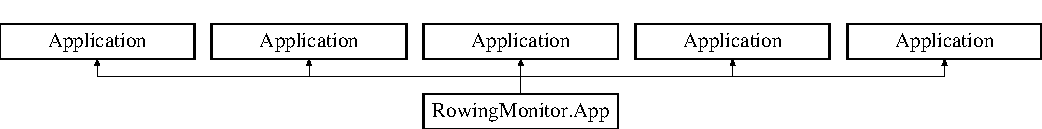
\includegraphics[height=1.709924cm]{class_rowing_monitor_1_1_app}
\end{center}
\end{figure}
\subsection*{Public Member Functions}
\begin{DoxyCompactItemize}
\item 
\hyperlink{class_rowing_monitor_1_1_app_a83d9e8a13163628ae72525843d35bbfe}{App} ()
\item 
void \hyperlink{class_rowing_monitor_1_1_app_a92cbce86d55626b5b411b795ec66c0c2}{Initialize\+Component} ()
\begin{DoxyCompactList}\small\item\em Initialize\+Component \end{DoxyCompactList}\item 
void \hyperlink{class_rowing_monitor_1_1_app_a92cbce86d55626b5b411b795ec66c0c2}{Initialize\+Component} ()
\begin{DoxyCompactList}\small\item\em Initialize\+Component \end{DoxyCompactList}\item 
void \hyperlink{class_rowing_monitor_1_1_app_a92cbce86d55626b5b411b795ec66c0c2}{Initialize\+Component} ()
\begin{DoxyCompactList}\small\item\em Initialize\+Component \end{DoxyCompactList}\item 
void \hyperlink{class_rowing_monitor_1_1_app_a92cbce86d55626b5b411b795ec66c0c2}{Initialize\+Component} ()
\begin{DoxyCompactList}\small\item\em Initialize\+Component \end{DoxyCompactList}\end{DoxyCompactItemize}
\subsection*{Static Public Member Functions}
\begin{DoxyCompactItemize}
\item 
static void \hyperlink{class_rowing_monitor_1_1_app_a3cb5b8569d044cd9687827e6c2072b7e}{Main} ()
\begin{DoxyCompactList}\small\item\em Application Entry Point. \end{DoxyCompactList}\item 
static void \hyperlink{class_rowing_monitor_1_1_app_a3cb5b8569d044cd9687827e6c2072b7e}{Main} ()
\begin{DoxyCompactList}\small\item\em Application Entry Point. \end{DoxyCompactList}\item 
static void \hyperlink{class_rowing_monitor_1_1_app_a3cb5b8569d044cd9687827e6c2072b7e}{Main} ()
\begin{DoxyCompactList}\small\item\em Application Entry Point. \end{DoxyCompactList}\item 
static void \hyperlink{class_rowing_monitor_1_1_app_a3cb5b8569d044cd9687827e6c2072b7e}{Main} ()
\begin{DoxyCompactList}\small\item\em Application Entry Point. \end{DoxyCompactList}\end{DoxyCompactItemize}
\subsection*{Protected Member Functions}
\begin{DoxyCompactItemize}
\item 
override void \hyperlink{class_rowing_monitor_1_1_app_a66e9b3baf5c2db1300758dddf3156f2f}{On\+Startup} (Startup\+Event\+Args e)
\end{DoxyCompactItemize}


\subsection{Detailed Description}
Interaktionslogik für \char`\"{}\+App.\+xaml\char`\"{} 

\hyperlink{class_rowing_monitor_1_1_app}{App} 

\subsection{Constructor \& Destructor Documentation}
\mbox{\Hypertarget{class_rowing_monitor_1_1_app_a83d9e8a13163628ae72525843d35bbfe}\label{class_rowing_monitor_1_1_app_a83d9e8a13163628ae72525843d35bbfe}} 
\index{Rowing\+Monitor\+::\+App@{Rowing\+Monitor\+::\+App}!App@{App}}
\index{App@{App}!Rowing\+Monitor\+::\+App@{Rowing\+Monitor\+::\+App}}
\subsubsection{\texorpdfstring{App()}{App()}}
{\footnotesize\ttfamily Rowing\+Monitor.\+App.\+App (\begin{DoxyParamCaption}{ }\end{DoxyParamCaption})}



\subsection{Member Function Documentation}
\mbox{\Hypertarget{class_rowing_monitor_1_1_app_a92cbce86d55626b5b411b795ec66c0c2}\label{class_rowing_monitor_1_1_app_a92cbce86d55626b5b411b795ec66c0c2}} 
\index{Rowing\+Monitor\+::\+App@{Rowing\+Monitor\+::\+App}!Initialize\+Component@{Initialize\+Component}}
\index{Initialize\+Component@{Initialize\+Component}!Rowing\+Monitor\+::\+App@{Rowing\+Monitor\+::\+App}}
\subsubsection{\texorpdfstring{Initialize\+Component()}{InitializeComponent()}\hspace{0.1cm}{\footnotesize\ttfamily [1/4]}}
{\footnotesize\ttfamily void Rowing\+Monitor.\+App.\+Initialize\+Component (\begin{DoxyParamCaption}{ }\end{DoxyParamCaption})}



Initialize\+Component 

\mbox{\Hypertarget{class_rowing_monitor_1_1_app_a92cbce86d55626b5b411b795ec66c0c2}\label{class_rowing_monitor_1_1_app_a92cbce86d55626b5b411b795ec66c0c2}} 
\index{Rowing\+Monitor\+::\+App@{Rowing\+Monitor\+::\+App}!Initialize\+Component@{Initialize\+Component}}
\index{Initialize\+Component@{Initialize\+Component}!Rowing\+Monitor\+::\+App@{Rowing\+Monitor\+::\+App}}
\subsubsection{\texorpdfstring{Initialize\+Component()}{InitializeComponent()}\hspace{0.1cm}{\footnotesize\ttfamily [2/4]}}
{\footnotesize\ttfamily void Rowing\+Monitor.\+App.\+Initialize\+Component (\begin{DoxyParamCaption}{ }\end{DoxyParamCaption})}



Initialize\+Component 

\mbox{\Hypertarget{class_rowing_monitor_1_1_app_a92cbce86d55626b5b411b795ec66c0c2}\label{class_rowing_monitor_1_1_app_a92cbce86d55626b5b411b795ec66c0c2}} 
\index{Rowing\+Monitor\+::\+App@{Rowing\+Monitor\+::\+App}!Initialize\+Component@{Initialize\+Component}}
\index{Initialize\+Component@{Initialize\+Component}!Rowing\+Monitor\+::\+App@{Rowing\+Monitor\+::\+App}}
\subsubsection{\texorpdfstring{Initialize\+Component()}{InitializeComponent()}\hspace{0.1cm}{\footnotesize\ttfamily [3/4]}}
{\footnotesize\ttfamily void Rowing\+Monitor.\+App.\+Initialize\+Component (\begin{DoxyParamCaption}{ }\end{DoxyParamCaption})}



Initialize\+Component 

\mbox{\Hypertarget{class_rowing_monitor_1_1_app_a92cbce86d55626b5b411b795ec66c0c2}\label{class_rowing_monitor_1_1_app_a92cbce86d55626b5b411b795ec66c0c2}} 
\index{Rowing\+Monitor\+::\+App@{Rowing\+Monitor\+::\+App}!Initialize\+Component@{Initialize\+Component}}
\index{Initialize\+Component@{Initialize\+Component}!Rowing\+Monitor\+::\+App@{Rowing\+Monitor\+::\+App}}
\subsubsection{\texorpdfstring{Initialize\+Component()}{InitializeComponent()}\hspace{0.1cm}{\footnotesize\ttfamily [4/4]}}
{\footnotesize\ttfamily void Rowing\+Monitor.\+App.\+Initialize\+Component (\begin{DoxyParamCaption}{ }\end{DoxyParamCaption})}



Initialize\+Component 

\mbox{\Hypertarget{class_rowing_monitor_1_1_app_a3cb5b8569d044cd9687827e6c2072b7e}\label{class_rowing_monitor_1_1_app_a3cb5b8569d044cd9687827e6c2072b7e}} 
\index{Rowing\+Monitor\+::\+App@{Rowing\+Monitor\+::\+App}!Main@{Main}}
\index{Main@{Main}!Rowing\+Monitor\+::\+App@{Rowing\+Monitor\+::\+App}}
\subsubsection{\texorpdfstring{Main()}{Main()}\hspace{0.1cm}{\footnotesize\ttfamily [1/4]}}
{\footnotesize\ttfamily static void Rowing\+Monitor.\+App.\+Main (\begin{DoxyParamCaption}{ }\end{DoxyParamCaption})\hspace{0.3cm}{\ttfamily [static]}}



Application Entry Point. 

\mbox{\Hypertarget{class_rowing_monitor_1_1_app_a3cb5b8569d044cd9687827e6c2072b7e}\label{class_rowing_monitor_1_1_app_a3cb5b8569d044cd9687827e6c2072b7e}} 
\index{Rowing\+Monitor\+::\+App@{Rowing\+Monitor\+::\+App}!Main@{Main}}
\index{Main@{Main}!Rowing\+Monitor\+::\+App@{Rowing\+Monitor\+::\+App}}
\subsubsection{\texorpdfstring{Main()}{Main()}\hspace{0.1cm}{\footnotesize\ttfamily [2/4]}}
{\footnotesize\ttfamily static void Rowing\+Monitor.\+App.\+Main (\begin{DoxyParamCaption}{ }\end{DoxyParamCaption})\hspace{0.3cm}{\ttfamily [static]}}



Application Entry Point. 

\mbox{\Hypertarget{class_rowing_monitor_1_1_app_a3cb5b8569d044cd9687827e6c2072b7e}\label{class_rowing_monitor_1_1_app_a3cb5b8569d044cd9687827e6c2072b7e}} 
\index{Rowing\+Monitor\+::\+App@{Rowing\+Monitor\+::\+App}!Main@{Main}}
\index{Main@{Main}!Rowing\+Monitor\+::\+App@{Rowing\+Monitor\+::\+App}}
\subsubsection{\texorpdfstring{Main()}{Main()}\hspace{0.1cm}{\footnotesize\ttfamily [3/4]}}
{\footnotesize\ttfamily static void Rowing\+Monitor.\+App.\+Main (\begin{DoxyParamCaption}{ }\end{DoxyParamCaption})\hspace{0.3cm}{\ttfamily [static]}}



Application Entry Point. 

\mbox{\Hypertarget{class_rowing_monitor_1_1_app_a3cb5b8569d044cd9687827e6c2072b7e}\label{class_rowing_monitor_1_1_app_a3cb5b8569d044cd9687827e6c2072b7e}} 
\index{Rowing\+Monitor\+::\+App@{Rowing\+Monitor\+::\+App}!Main@{Main}}
\index{Main@{Main}!Rowing\+Monitor\+::\+App@{Rowing\+Monitor\+::\+App}}
\subsubsection{\texorpdfstring{Main()}{Main()}\hspace{0.1cm}{\footnotesize\ttfamily [4/4]}}
{\footnotesize\ttfamily static void Rowing\+Monitor.\+App.\+Main (\begin{DoxyParamCaption}{ }\end{DoxyParamCaption})\hspace{0.3cm}{\ttfamily [static]}}



Application Entry Point. 

\mbox{\Hypertarget{class_rowing_monitor_1_1_app_a66e9b3baf5c2db1300758dddf3156f2f}\label{class_rowing_monitor_1_1_app_a66e9b3baf5c2db1300758dddf3156f2f}} 
\index{Rowing\+Monitor\+::\+App@{Rowing\+Monitor\+::\+App}!On\+Startup@{On\+Startup}}
\index{On\+Startup@{On\+Startup}!Rowing\+Monitor\+::\+App@{Rowing\+Monitor\+::\+App}}
\subsubsection{\texorpdfstring{On\+Startup()}{OnStartup()}}
{\footnotesize\ttfamily override void Rowing\+Monitor.\+App.\+On\+Startup (\begin{DoxyParamCaption}\item[{Startup\+Event\+Args}]{e }\end{DoxyParamCaption})\hspace{0.3cm}{\ttfamily [protected]}}



The documentation for this class was generated from the following files\+:\begin{DoxyCompactItemize}
\item 
\hyperlink{_app_8xaml_8cs}{App.\+xaml.\+cs}\item 
obj/\+Debug/\hyperlink{_debug_2_app_8g_8cs}{App.\+g.\+cs}\item 
obj/\+Debug/\hyperlink{_debug_2_app_8g_8i_8cs}{App.\+g.\+i.\+cs}\end{DoxyCompactItemize}

\hypertarget{class_rowing_monitor_1_1_model_1_1_body_not_fully_tracked_exception}{}\section{Rowing\+Monitor.\+Model.\+Body\+Not\+Fully\+Tracked\+Exception Class Reference}
\label{class_rowing_monitor_1_1_model_1_1_body_not_fully_tracked_exception}\index{Rowing\+Monitor.\+Model.\+Body\+Not\+Fully\+Tracked\+Exception@{Rowing\+Monitor.\+Model.\+Body\+Not\+Fully\+Tracked\+Exception}}
Inheritance diagram for Rowing\+Monitor.\+Model.\+Body\+Not\+Fully\+Tracked\+Exception\+:\begin{figure}[H]
\begin{center}
\leavevmode
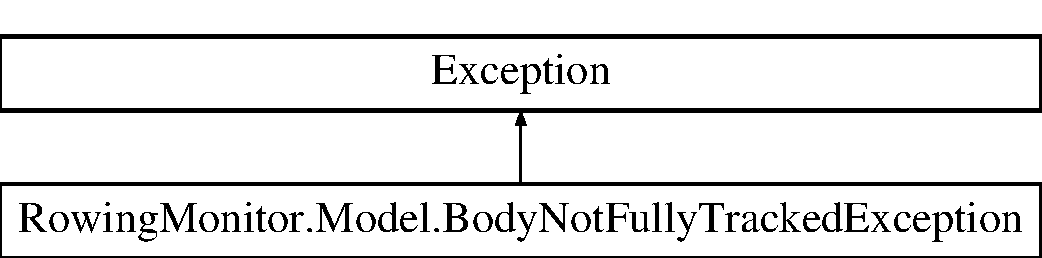
\includegraphics[height=2.000000cm]{class_rowing_monitor_1_1_model_1_1_body_not_fully_tracked_exception}
\end{center}
\end{figure}


The documentation for this class was generated from the following file\+:\begin{DoxyCompactItemize}
\item 
Model/\+Util/\hyperlink{_body_not_fully_tracked_exception_8cs}{Body\+Not\+Fully\+Tracked\+Exception.\+cs}\end{DoxyCompactItemize}

\hypertarget{class_rowing_monitor_1_1_model_1_1_calculated_frame_arrived_event_args}{}\section{Rowing\+Monitor.\+Model.\+Calculated\+Frame\+Arrived\+Event\+Args Class Reference}
\label{class_rowing_monitor_1_1_model_1_1_calculated_frame_arrived_event_args}\index{Rowing\+Monitor.\+Model.\+Calculated\+Frame\+Arrived\+Event\+Args@{Rowing\+Monitor.\+Model.\+Calculated\+Frame\+Arrived\+Event\+Args}}


Represents the arguments for a calculated frame arrived event.  


Inheritance diagram for Rowing\+Monitor.\+Model.\+Calculated\+Frame\+Arrived\+Event\+Args\+:\begin{figure}[H]
\begin{center}
\leavevmode
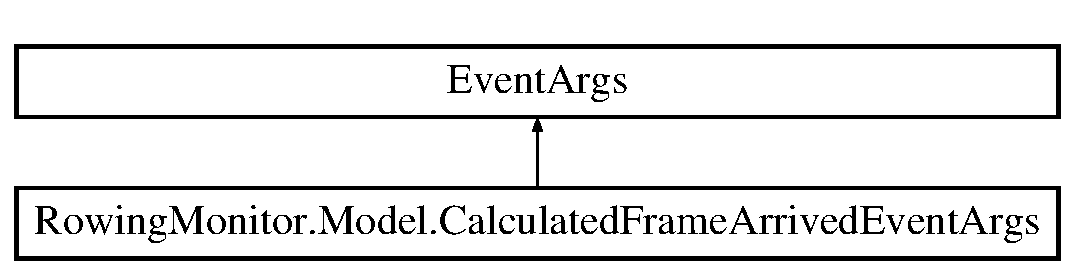
\includegraphics[height=2.000000cm]{class_rowing_monitor_1_1_model_1_1_calculated_frame_arrived_event_args}
\end{center}
\end{figure}
\subsection*{Public Member Functions}
\begin{DoxyCompactItemize}
\item 
\hyperlink{class_rowing_monitor_1_1_model_1_1_calculated_frame_arrived_event_args_ab73cb44f37b699c76ed2a5b1d98338d3}{Calculated\+Frame\+Arrived\+Event\+Args} (\hyperlink{struct_rowing_monitor_1_1_model_1_1_util_1_1_joint_data}{Joint\+Data} calculated\+Joint\+Data)
\end{DoxyCompactItemize}
\subsection*{Properties}
\begin{DoxyCompactItemize}
\item 
\hyperlink{struct_rowing_monitor_1_1_model_1_1_util_1_1_joint_data}{Joint\+Data} \hyperlink{class_rowing_monitor_1_1_model_1_1_calculated_frame_arrived_event_args_ad2a6d96247f32cec46b5e5006b4a867b}{Calculated\+Joint\+Data}\hspace{0.3cm}{\ttfamily  \mbox{[}get\mbox{]}}
\end{DoxyCompactItemize}


\subsection{Detailed Description}
Represents the arguments for a calculated frame arrived event. 



\subsection{Constructor \& Destructor Documentation}
\mbox{\Hypertarget{class_rowing_monitor_1_1_model_1_1_calculated_frame_arrived_event_args_ab73cb44f37b699c76ed2a5b1d98338d3}\label{class_rowing_monitor_1_1_model_1_1_calculated_frame_arrived_event_args_ab73cb44f37b699c76ed2a5b1d98338d3}} 
\index{Rowing\+Monitor\+::\+Model\+::\+Calculated\+Frame\+Arrived\+Event\+Args@{Rowing\+Monitor\+::\+Model\+::\+Calculated\+Frame\+Arrived\+Event\+Args}!Calculated\+Frame\+Arrived\+Event\+Args@{Calculated\+Frame\+Arrived\+Event\+Args}}
\index{Calculated\+Frame\+Arrived\+Event\+Args@{Calculated\+Frame\+Arrived\+Event\+Args}!Rowing\+Monitor\+::\+Model\+::\+Calculated\+Frame\+Arrived\+Event\+Args@{Rowing\+Monitor\+::\+Model\+::\+Calculated\+Frame\+Arrived\+Event\+Args}}
\subsubsection{\texorpdfstring{Calculated\+Frame\+Arrived\+Event\+Args()}{CalculatedFrameArrivedEventArgs()}}
{\footnotesize\ttfamily Rowing\+Monitor.\+Model.\+Calculated\+Frame\+Arrived\+Event\+Args.\+Calculated\+Frame\+Arrived\+Event\+Args (\begin{DoxyParamCaption}\item[{\hyperlink{struct_rowing_monitor_1_1_model_1_1_util_1_1_joint_data}{Joint\+Data}}]{calculated\+Joint\+Data }\end{DoxyParamCaption})}



\subsection{Property Documentation}
\mbox{\Hypertarget{class_rowing_monitor_1_1_model_1_1_calculated_frame_arrived_event_args_ad2a6d96247f32cec46b5e5006b4a867b}\label{class_rowing_monitor_1_1_model_1_1_calculated_frame_arrived_event_args_ad2a6d96247f32cec46b5e5006b4a867b}} 
\index{Rowing\+Monitor\+::\+Model\+::\+Calculated\+Frame\+Arrived\+Event\+Args@{Rowing\+Monitor\+::\+Model\+::\+Calculated\+Frame\+Arrived\+Event\+Args}!Calculated\+Joint\+Data@{Calculated\+Joint\+Data}}
\index{Calculated\+Joint\+Data@{Calculated\+Joint\+Data}!Rowing\+Monitor\+::\+Model\+::\+Calculated\+Frame\+Arrived\+Event\+Args@{Rowing\+Monitor\+::\+Model\+::\+Calculated\+Frame\+Arrived\+Event\+Args}}
\subsubsection{\texorpdfstring{Calculated\+Joint\+Data}{CalculatedJointData}}
{\footnotesize\ttfamily \hyperlink{struct_rowing_monitor_1_1_model_1_1_util_1_1_joint_data}{Joint\+Data} Rowing\+Monitor.\+Model.\+Calculated\+Frame\+Arrived\+Event\+Args.\+Calculated\+Joint\+Data\hspace{0.3cm}{\ttfamily [get]}}



The documentation for this class was generated from the following file\+:\begin{DoxyCompactItemize}
\item 
Model/\+Event\+Args/\hyperlink{_calculated_frame_arrived_event_args_8cs}{Calculated\+Frame\+Arrived\+Event\+Args.\+cs}\end{DoxyCompactItemize}

\hypertarget{class_rowing_monitor_1_1_model_1_1_color_frame_arrived_event_args}{}\section{Rowing\+Monitor.\+Model.\+Color\+Frame\+Arrived\+Event\+Args Class Reference}
\label{class_rowing_monitor_1_1_model_1_1_color_frame_arrived_event_args}\index{Rowing\+Monitor.\+Model.\+Color\+Frame\+Arrived\+Event\+Args@{Rowing\+Monitor.\+Model.\+Color\+Frame\+Arrived\+Event\+Args}}


Represents the arguments for a \hyperlink{class_rowing_monitor_1_1_model_1_1_kinect_reader}{Kinect\+Reader}\textquotesingle{}s Color\+Frame\+Arrived event.  


Inheritance diagram for Rowing\+Monitor.\+Model.\+Color\+Frame\+Arrived\+Event\+Args\+:\begin{figure}[H]
\begin{center}
\leavevmode
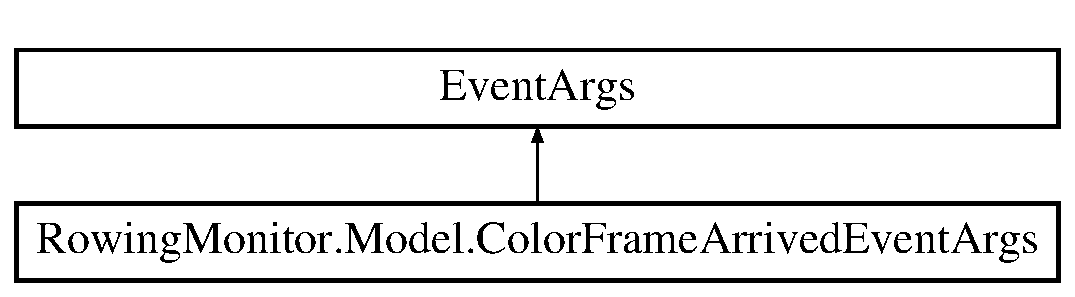
\includegraphics[height=2.000000cm]{class_rowing_monitor_1_1_model_1_1_color_frame_arrived_event_args}
\end{center}
\end{figure}
\subsection*{Public Member Functions}
\begin{DoxyCompactItemize}
\item 
\hyperlink{class_rowing_monitor_1_1_model_1_1_color_frame_arrived_event_args_a228785b0fda3657a17d7c30fd429ba1c}{Color\+Frame\+Arrived\+Event\+Args} (Writeable\+Bitmap color\+Bitmap)
\end{DoxyCompactItemize}
\subsection*{Properties}
\begin{DoxyCompactItemize}
\item 
Writeable\+Bitmap \hyperlink{class_rowing_monitor_1_1_model_1_1_color_frame_arrived_event_args_a2332327334320a56103d13596128a841}{Color\+Bitmap}\hspace{0.3cm}{\ttfamily  \mbox{[}get\mbox{]}}
\end{DoxyCompactItemize}


\subsection{Detailed Description}
Represents the arguments for a \hyperlink{class_rowing_monitor_1_1_model_1_1_kinect_reader}{Kinect\+Reader}\textquotesingle{}s Color\+Frame\+Arrived event. 



\subsection{Constructor \& Destructor Documentation}
\mbox{\Hypertarget{class_rowing_monitor_1_1_model_1_1_color_frame_arrived_event_args_a228785b0fda3657a17d7c30fd429ba1c}\label{class_rowing_monitor_1_1_model_1_1_color_frame_arrived_event_args_a228785b0fda3657a17d7c30fd429ba1c}} 
\index{Rowing\+Monitor\+::\+Model\+::\+Color\+Frame\+Arrived\+Event\+Args@{Rowing\+Monitor\+::\+Model\+::\+Color\+Frame\+Arrived\+Event\+Args}!Color\+Frame\+Arrived\+Event\+Args@{Color\+Frame\+Arrived\+Event\+Args}}
\index{Color\+Frame\+Arrived\+Event\+Args@{Color\+Frame\+Arrived\+Event\+Args}!Rowing\+Monitor\+::\+Model\+::\+Color\+Frame\+Arrived\+Event\+Args@{Rowing\+Monitor\+::\+Model\+::\+Color\+Frame\+Arrived\+Event\+Args}}
\subsubsection{\texorpdfstring{Color\+Frame\+Arrived\+Event\+Args()}{ColorFrameArrivedEventArgs()}}
{\footnotesize\ttfamily Rowing\+Monitor.\+Model.\+Color\+Frame\+Arrived\+Event\+Args.\+Color\+Frame\+Arrived\+Event\+Args (\begin{DoxyParamCaption}\item[{Writeable\+Bitmap}]{color\+Bitmap }\end{DoxyParamCaption})}



\subsection{Property Documentation}
\mbox{\Hypertarget{class_rowing_monitor_1_1_model_1_1_color_frame_arrived_event_args_a2332327334320a56103d13596128a841}\label{class_rowing_monitor_1_1_model_1_1_color_frame_arrived_event_args_a2332327334320a56103d13596128a841}} 
\index{Rowing\+Monitor\+::\+Model\+::\+Color\+Frame\+Arrived\+Event\+Args@{Rowing\+Monitor\+::\+Model\+::\+Color\+Frame\+Arrived\+Event\+Args}!Color\+Bitmap@{Color\+Bitmap}}
\index{Color\+Bitmap@{Color\+Bitmap}!Rowing\+Monitor\+::\+Model\+::\+Color\+Frame\+Arrived\+Event\+Args@{Rowing\+Monitor\+::\+Model\+::\+Color\+Frame\+Arrived\+Event\+Args}}
\subsubsection{\texorpdfstring{Color\+Bitmap}{ColorBitmap}}
{\footnotesize\ttfamily Writeable\+Bitmap Rowing\+Monitor.\+Model.\+Color\+Frame\+Arrived\+Event\+Args.\+Color\+Bitmap\hspace{0.3cm}{\ttfamily [get]}}



The documentation for this class was generated from the following file\+:\begin{DoxyCompactItemize}
\item 
Model/\+Event\+Args/\hyperlink{_color_frame_arrived_event_args_8cs}{Color\+Frame\+Arrived\+Event\+Args.\+cs}\end{DoxyCompactItemize}

\hypertarget{class_rowing_monitor_1_1_model_1_1_pipeline_1_1_d_t_w_segment_detector}{}\section{Rowing\+Monitor.\+Model.\+Pipeline.\+D\+T\+W\+Segment\+Detector Class Reference}
\label{class_rowing_monitor_1_1_model_1_1_pipeline_1_1_d_t_w_segment_detector}\index{Rowing\+Monitor.\+Model.\+Pipeline.\+D\+T\+W\+Segment\+Detector@{Rowing\+Monitor.\+Model.\+Pipeline.\+D\+T\+W\+Segment\+Detector}}
Inheritance diagram for Rowing\+Monitor.\+Model.\+Pipeline.\+D\+T\+W\+Segment\+Detector\+:\begin{figure}[H]
\begin{center}
\leavevmode
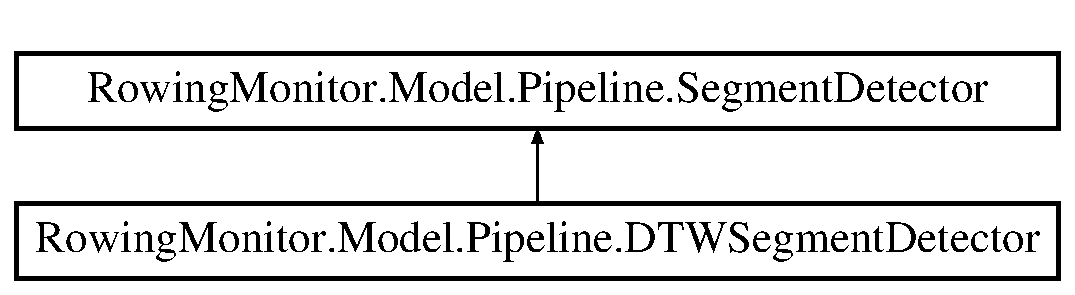
\includegraphics[height=2.000000cm]{class_rowing_monitor_1_1_model_1_1_pipeline_1_1_d_t_w_segment_detector}
\end{center}
\end{figure}
\subsection*{Public Member Functions}
\begin{DoxyCompactItemize}
\item 
\hyperlink{class_rowing_monitor_1_1_model_1_1_pipeline_1_1_d_t_w_segment_detector_abfb0a6199eaaf5bb079bbcf1c2eaecc5}{D\+T\+W\+Segment\+Detector} (float distance\+Threshold, int minimum\+Subsequence\+Length)
\item 
override void \hyperlink{class_rowing_monitor_1_1_model_1_1_pipeline_1_1_d_t_w_segment_detector_a211aec92693f8a229d88dd6a5b059eb4}{Update} (\hyperlink{struct_rowing_monitor_1_1_model_1_1_util_1_1_joint_data}{Joint\+Data} joint\+Data, Joint\+Type joint\+Type, string axis)
\item 
override List$<$ \hyperlink{struct_rowing_monitor_1_1_model_1_1_util_1_1_segment_hit}{Segment\+Hit} $>$ \hyperlink{class_rowing_monitor_1_1_model_1_1_pipeline_1_1_d_t_w_segment_detector_ab65c258b405b4a73e22ea114173965a6}{Detect} (\hyperlink{struct_rowing_monitor_1_1_model_1_1_util_1_1_joint_data}{Joint\+Data} joint\+Data, Joint\+Type joint\+Type, string axis)
\end{DoxyCompactItemize}
\subsection*{Protected Member Functions}
\begin{DoxyCompactItemize}
\item 
override void \hyperlink{class_rowing_monitor_1_1_model_1_1_pipeline_1_1_d_t_w_segment_detector_a6d2644f751e290cef82649c42becdd92}{On\+Segment\+Detected} (\hyperlink{class_rowing_monitor_1_1_model_1_1_segment_detected_event_args}{Segment\+Detected\+Event\+Args} e)
\end{DoxyCompactItemize}
\subsection*{Additional Inherited Members}


\subsection{Constructor \& Destructor Documentation}
\mbox{\Hypertarget{class_rowing_monitor_1_1_model_1_1_pipeline_1_1_d_t_w_segment_detector_abfb0a6199eaaf5bb079bbcf1c2eaecc5}\label{class_rowing_monitor_1_1_model_1_1_pipeline_1_1_d_t_w_segment_detector_abfb0a6199eaaf5bb079bbcf1c2eaecc5}} 
\index{Rowing\+Monitor\+::\+Model\+::\+Pipeline\+::\+D\+T\+W\+Segment\+Detector@{Rowing\+Monitor\+::\+Model\+::\+Pipeline\+::\+D\+T\+W\+Segment\+Detector}!D\+T\+W\+Segment\+Detector@{D\+T\+W\+Segment\+Detector}}
\index{D\+T\+W\+Segment\+Detector@{D\+T\+W\+Segment\+Detector}!Rowing\+Monitor\+::\+Model\+::\+Pipeline\+::\+D\+T\+W\+Segment\+Detector@{Rowing\+Monitor\+::\+Model\+::\+Pipeline\+::\+D\+T\+W\+Segment\+Detector}}
\subsubsection{\texorpdfstring{D\+T\+W\+Segment\+Detector()}{DTWSegmentDetector()}}
{\footnotesize\ttfamily Rowing\+Monitor.\+Model.\+Pipeline.\+D\+T\+W\+Segment\+Detector.\+D\+T\+W\+Segment\+Detector (\begin{DoxyParamCaption}\item[{float}]{distance\+Threshold,  }\item[{int}]{minimum\+Subsequence\+Length }\end{DoxyParamCaption})}



\subsection{Member Function Documentation}
\mbox{\Hypertarget{class_rowing_monitor_1_1_model_1_1_pipeline_1_1_d_t_w_segment_detector_ab65c258b405b4a73e22ea114173965a6}\label{class_rowing_monitor_1_1_model_1_1_pipeline_1_1_d_t_w_segment_detector_ab65c258b405b4a73e22ea114173965a6}} 
\index{Rowing\+Monitor\+::\+Model\+::\+Pipeline\+::\+D\+T\+W\+Segment\+Detector@{Rowing\+Monitor\+::\+Model\+::\+Pipeline\+::\+D\+T\+W\+Segment\+Detector}!Detect@{Detect}}
\index{Detect@{Detect}!Rowing\+Monitor\+::\+Model\+::\+Pipeline\+::\+D\+T\+W\+Segment\+Detector@{Rowing\+Monitor\+::\+Model\+::\+Pipeline\+::\+D\+T\+W\+Segment\+Detector}}
\subsubsection{\texorpdfstring{Detect()}{Detect()}}
{\footnotesize\ttfamily override List$<$\hyperlink{struct_rowing_monitor_1_1_model_1_1_util_1_1_segment_hit}{Segment\+Hit}$>$ Rowing\+Monitor.\+Model.\+Pipeline.\+D\+T\+W\+Segment\+Detector.\+Detect (\begin{DoxyParamCaption}\item[{\hyperlink{struct_rowing_monitor_1_1_model_1_1_util_1_1_joint_data}{Joint\+Data}}]{joint\+Data,  }\item[{Joint\+Type}]{joint\+Type,  }\item[{string}]{axis }\end{DoxyParamCaption})}

\mbox{\Hypertarget{class_rowing_monitor_1_1_model_1_1_pipeline_1_1_d_t_w_segment_detector_a6d2644f751e290cef82649c42becdd92}\label{class_rowing_monitor_1_1_model_1_1_pipeline_1_1_d_t_w_segment_detector_a6d2644f751e290cef82649c42becdd92}} 
\index{Rowing\+Monitor\+::\+Model\+::\+Pipeline\+::\+D\+T\+W\+Segment\+Detector@{Rowing\+Monitor\+::\+Model\+::\+Pipeline\+::\+D\+T\+W\+Segment\+Detector}!On\+Segment\+Detected@{On\+Segment\+Detected}}
\index{On\+Segment\+Detected@{On\+Segment\+Detected}!Rowing\+Monitor\+::\+Model\+::\+Pipeline\+::\+D\+T\+W\+Segment\+Detector@{Rowing\+Monitor\+::\+Model\+::\+Pipeline\+::\+D\+T\+W\+Segment\+Detector}}
\subsubsection{\texorpdfstring{On\+Segment\+Detected()}{OnSegmentDetected()}}
{\footnotesize\ttfamily override void Rowing\+Monitor.\+Model.\+Pipeline.\+D\+T\+W\+Segment\+Detector.\+On\+Segment\+Detected (\begin{DoxyParamCaption}\item[{\hyperlink{class_rowing_monitor_1_1_model_1_1_segment_detected_event_args}{Segment\+Detected\+Event\+Args}}]{e }\end{DoxyParamCaption})\hspace{0.3cm}{\ttfamily [protected]}, {\ttfamily [virtual]}}



Reimplemented from \hyperlink{class_rowing_monitor_1_1_model_1_1_pipeline_1_1_segment_detector_a30d5b8752257a3992db11770506f6a8a}{Rowing\+Monitor.\+Model.\+Pipeline.\+Segment\+Detector}.

\mbox{\Hypertarget{class_rowing_monitor_1_1_model_1_1_pipeline_1_1_d_t_w_segment_detector_a211aec92693f8a229d88dd6a5b059eb4}\label{class_rowing_monitor_1_1_model_1_1_pipeline_1_1_d_t_w_segment_detector_a211aec92693f8a229d88dd6a5b059eb4}} 
\index{Rowing\+Monitor\+::\+Model\+::\+Pipeline\+::\+D\+T\+W\+Segment\+Detector@{Rowing\+Monitor\+::\+Model\+::\+Pipeline\+::\+D\+T\+W\+Segment\+Detector}!Update@{Update}}
\index{Update@{Update}!Rowing\+Monitor\+::\+Model\+::\+Pipeline\+::\+D\+T\+W\+Segment\+Detector@{Rowing\+Monitor\+::\+Model\+::\+Pipeline\+::\+D\+T\+W\+Segment\+Detector}}
\subsubsection{\texorpdfstring{Update()}{Update()}}
{\footnotesize\ttfamily override void Rowing\+Monitor.\+Model.\+Pipeline.\+D\+T\+W\+Segment\+Detector.\+Update (\begin{DoxyParamCaption}\item[{\hyperlink{struct_rowing_monitor_1_1_model_1_1_util_1_1_joint_data}{Joint\+Data}}]{joint\+Data,  }\item[{Joint\+Type}]{joint\+Type,  }\item[{string}]{axis }\end{DoxyParamCaption})}



The documentation for this class was generated from the following file\+:\begin{DoxyCompactItemize}
\item 
Model/\+Pipeline/\hyperlink{_d_t_w_segment_detector_8cs}{D\+T\+W\+Segment\+Detector.\+cs}\end{DoxyCompactItemize}

\hypertarget{class_rowing_monitor_1_1_model_1_1_pipeline_1_1_kinect_joint_filter_1_1_filter_double_exponential_data}{}\section{Rowing\+Monitor.\+Model.\+Pipeline.\+Kinect\+Joint\+Filter.\+Filter\+Double\+Exponential\+Data Class Reference}
\label{class_rowing_monitor_1_1_model_1_1_pipeline_1_1_kinect_joint_filter_1_1_filter_double_exponential_data}\index{Rowing\+Monitor.\+Model.\+Pipeline.\+Kinect\+Joint\+Filter.\+Filter\+Double\+Exponential\+Data@{Rowing\+Monitor.\+Model.\+Pipeline.\+Kinect\+Joint\+Filter.\+Filter\+Double\+Exponential\+Data}}
\subsection*{Public Attributes}
\begin{DoxyCompactItemize}
\item 
Camera\+Space\+Point \hyperlink{class_rowing_monitor_1_1_model_1_1_pipeline_1_1_kinect_joint_filter_1_1_filter_double_exponential_data_a4b4b473d842af471a1a255435389942d}{m\+\_\+v\+Raw\+Position}
\item 
Camera\+Space\+Point \hyperlink{class_rowing_monitor_1_1_model_1_1_pipeline_1_1_kinect_joint_filter_1_1_filter_double_exponential_data_a7a0450af4adf9ba3725a9abfc5974b7b}{m\+\_\+v\+Filtered\+Position}
\item 
Camera\+Space\+Point \hyperlink{class_rowing_monitor_1_1_model_1_1_pipeline_1_1_kinect_joint_filter_1_1_filter_double_exponential_data_a1e769a54b1aed666aa8ea9b331b20ff0}{m\+\_\+v\+Trend}
\item 
int \hyperlink{class_rowing_monitor_1_1_model_1_1_pipeline_1_1_kinect_joint_filter_1_1_filter_double_exponential_data_af24ed5a40f362c56649cfc8306c0f643}{m\+\_\+dw\+Frame\+Count}
\end{DoxyCompactItemize}


\subsection{Member Data Documentation}
\mbox{\Hypertarget{class_rowing_monitor_1_1_model_1_1_pipeline_1_1_kinect_joint_filter_1_1_filter_double_exponential_data_af24ed5a40f362c56649cfc8306c0f643}\label{class_rowing_monitor_1_1_model_1_1_pipeline_1_1_kinect_joint_filter_1_1_filter_double_exponential_data_af24ed5a40f362c56649cfc8306c0f643}} 
\index{Rowing\+Monitor\+::\+Model\+::\+Pipeline\+::\+Kinect\+Joint\+Filter\+::\+Filter\+Double\+Exponential\+Data@{Rowing\+Monitor\+::\+Model\+::\+Pipeline\+::\+Kinect\+Joint\+Filter\+::\+Filter\+Double\+Exponential\+Data}!m\+\_\+dw\+Frame\+Count@{m\+\_\+dw\+Frame\+Count}}
\index{m\+\_\+dw\+Frame\+Count@{m\+\_\+dw\+Frame\+Count}!Rowing\+Monitor\+::\+Model\+::\+Pipeline\+::\+Kinect\+Joint\+Filter\+::\+Filter\+Double\+Exponential\+Data@{Rowing\+Monitor\+::\+Model\+::\+Pipeline\+::\+Kinect\+Joint\+Filter\+::\+Filter\+Double\+Exponential\+Data}}
\subsubsection{\texorpdfstring{m\+\_\+dw\+Frame\+Count}{m\_dwFrameCount}}
{\footnotesize\ttfamily int Rowing\+Monitor.\+Model.\+Pipeline.\+Kinect\+Joint\+Filter.\+Filter\+Double\+Exponential\+Data.\+m\+\_\+dw\+Frame\+Count}

\mbox{\Hypertarget{class_rowing_monitor_1_1_model_1_1_pipeline_1_1_kinect_joint_filter_1_1_filter_double_exponential_data_a7a0450af4adf9ba3725a9abfc5974b7b}\label{class_rowing_monitor_1_1_model_1_1_pipeline_1_1_kinect_joint_filter_1_1_filter_double_exponential_data_a7a0450af4adf9ba3725a9abfc5974b7b}} 
\index{Rowing\+Monitor\+::\+Model\+::\+Pipeline\+::\+Kinect\+Joint\+Filter\+::\+Filter\+Double\+Exponential\+Data@{Rowing\+Monitor\+::\+Model\+::\+Pipeline\+::\+Kinect\+Joint\+Filter\+::\+Filter\+Double\+Exponential\+Data}!m\+\_\+v\+Filtered\+Position@{m\+\_\+v\+Filtered\+Position}}
\index{m\+\_\+v\+Filtered\+Position@{m\+\_\+v\+Filtered\+Position}!Rowing\+Monitor\+::\+Model\+::\+Pipeline\+::\+Kinect\+Joint\+Filter\+::\+Filter\+Double\+Exponential\+Data@{Rowing\+Monitor\+::\+Model\+::\+Pipeline\+::\+Kinect\+Joint\+Filter\+::\+Filter\+Double\+Exponential\+Data}}
\subsubsection{\texorpdfstring{m\+\_\+v\+Filtered\+Position}{m\_vFilteredPosition}}
{\footnotesize\ttfamily Camera\+Space\+Point Rowing\+Monitor.\+Model.\+Pipeline.\+Kinect\+Joint\+Filter.\+Filter\+Double\+Exponential\+Data.\+m\+\_\+v\+Filtered\+Position}

\mbox{\Hypertarget{class_rowing_monitor_1_1_model_1_1_pipeline_1_1_kinect_joint_filter_1_1_filter_double_exponential_data_a4b4b473d842af471a1a255435389942d}\label{class_rowing_monitor_1_1_model_1_1_pipeline_1_1_kinect_joint_filter_1_1_filter_double_exponential_data_a4b4b473d842af471a1a255435389942d}} 
\index{Rowing\+Monitor\+::\+Model\+::\+Pipeline\+::\+Kinect\+Joint\+Filter\+::\+Filter\+Double\+Exponential\+Data@{Rowing\+Monitor\+::\+Model\+::\+Pipeline\+::\+Kinect\+Joint\+Filter\+::\+Filter\+Double\+Exponential\+Data}!m\+\_\+v\+Raw\+Position@{m\+\_\+v\+Raw\+Position}}
\index{m\+\_\+v\+Raw\+Position@{m\+\_\+v\+Raw\+Position}!Rowing\+Monitor\+::\+Model\+::\+Pipeline\+::\+Kinect\+Joint\+Filter\+::\+Filter\+Double\+Exponential\+Data@{Rowing\+Monitor\+::\+Model\+::\+Pipeline\+::\+Kinect\+Joint\+Filter\+::\+Filter\+Double\+Exponential\+Data}}
\subsubsection{\texorpdfstring{m\+\_\+v\+Raw\+Position}{m\_vRawPosition}}
{\footnotesize\ttfamily Camera\+Space\+Point Rowing\+Monitor.\+Model.\+Pipeline.\+Kinect\+Joint\+Filter.\+Filter\+Double\+Exponential\+Data.\+m\+\_\+v\+Raw\+Position}

\mbox{\Hypertarget{class_rowing_monitor_1_1_model_1_1_pipeline_1_1_kinect_joint_filter_1_1_filter_double_exponential_data_a1e769a54b1aed666aa8ea9b331b20ff0}\label{class_rowing_monitor_1_1_model_1_1_pipeline_1_1_kinect_joint_filter_1_1_filter_double_exponential_data_a1e769a54b1aed666aa8ea9b331b20ff0}} 
\index{Rowing\+Monitor\+::\+Model\+::\+Pipeline\+::\+Kinect\+Joint\+Filter\+::\+Filter\+Double\+Exponential\+Data@{Rowing\+Monitor\+::\+Model\+::\+Pipeline\+::\+Kinect\+Joint\+Filter\+::\+Filter\+Double\+Exponential\+Data}!m\+\_\+v\+Trend@{m\+\_\+v\+Trend}}
\index{m\+\_\+v\+Trend@{m\+\_\+v\+Trend}!Rowing\+Monitor\+::\+Model\+::\+Pipeline\+::\+Kinect\+Joint\+Filter\+::\+Filter\+Double\+Exponential\+Data@{Rowing\+Monitor\+::\+Model\+::\+Pipeline\+::\+Kinect\+Joint\+Filter\+::\+Filter\+Double\+Exponential\+Data}}
\subsubsection{\texorpdfstring{m\+\_\+v\+Trend}{m\_vTrend}}
{\footnotesize\ttfamily Camera\+Space\+Point Rowing\+Monitor.\+Model.\+Pipeline.\+Kinect\+Joint\+Filter.\+Filter\+Double\+Exponential\+Data.\+m\+\_\+v\+Trend}



The documentation for this class was generated from the following file\+:\begin{DoxyCompactItemize}
\item 
Model/\+Pipeline/\hyperlink{_kinect_joint_filter_8cs}{Kinect\+Joint\+Filter.\+cs}\end{DoxyCompactItemize}

\hypertarget{class_rowing_monitor_1_1_model_1_1_frontal_view}{}\section{Rowing\+Monitor.\+Model.\+Frontal\+View Class Reference}
\label{class_rowing_monitor_1_1_model_1_1_frontal_view}\index{Rowing\+Monitor.\+Model.\+Frontal\+View@{Rowing\+Monitor.\+Model.\+Frontal\+View}}


This class shows a frontal view of the tracked skeleton. Also it shows the color image sequence which is recorded by the kinect sensor.  


Inheritance diagram for Rowing\+Monitor.\+Model.\+Frontal\+View\+:\begin{figure}[H]
\begin{center}
\leavevmode
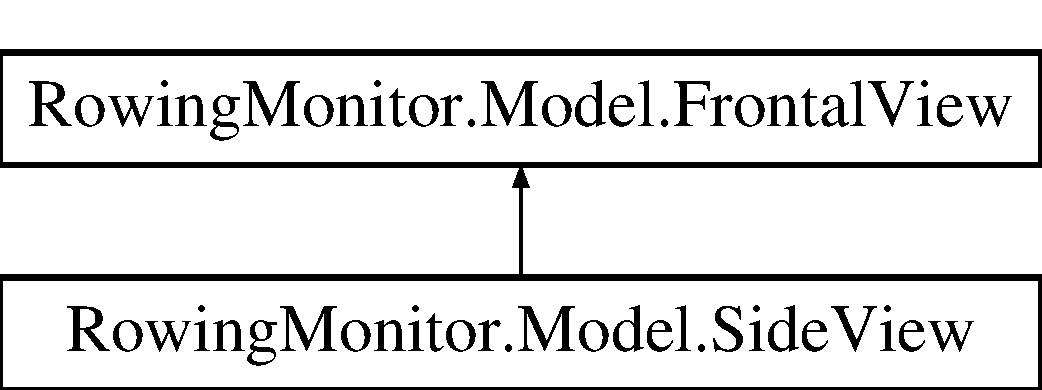
\includegraphics[height=2.000000cm]{class_rowing_monitor_1_1_model_1_1_frontal_view}
\end{center}
\end{figure}
\subsection*{Public Member Functions}
\begin{DoxyCompactItemize}
\item 
\hyperlink{class_rowing_monitor_1_1_model_1_1_frontal_view_aa02b93cf606fc1d6fb0159ed39a53f5c}{Frontal\+View} (Coordinate\+Mapper mapper, int width, int height)
\item 
virtual void \hyperlink{class_rowing_monitor_1_1_model_1_1_frontal_view_a3dddfa75ba346fdcf99dbd763e9ea1ea}{Update\+Skeleton} (I\+Read\+Only\+Dictionary$<$ Joint\+Type, Joint $>$ joints)
\begin{DoxyCompactList}\small\item\em Updates the view with new data. \end{DoxyCompactList}\item 
void \hyperlink{class_rowing_monitor_1_1_model_1_1_frontal_view_aa1fda6d35d7fa125830ce5c9c64f92d5}{Update\+Color\+Image} (Writeable\+Bitmap color\+Image)
\end{DoxyCompactItemize}
\subsection*{Protected Member Functions}
\begin{DoxyCompactItemize}
\item 
void \hyperlink{class_rowing_monitor_1_1_model_1_1_frontal_view_af65ccffe0927daa614219f7db3765831}{Draw\+Body} (I\+Read\+Only\+Dictionary$<$ Joint\+Type, Joint $>$ joints, I\+Dictionary$<$ Joint\+Type, Point $>$ joint\+Points, Drawing\+Context drawing\+Context, Pen drawing\+Pen)
\begin{DoxyCompactList}\small\item\em Draws a body \end{DoxyCompactList}\end{DoxyCompactItemize}
\subsection*{Protected Attributes}
\begin{DoxyCompactItemize}
\item 
const double \hyperlink{class_rowing_monitor_1_1_model_1_1_frontal_view_af0d4024f6496a4408e27f1d7bb4327b8}{Joint\+Thickness} = 3
\begin{DoxyCompactList}\small\item\em Thickness of drawn joint lines \end{DoxyCompactList}\item 
const float \hyperlink{class_rowing_monitor_1_1_model_1_1_frontal_view_a5f663eb0eda7d5561022fa1b048ff28c}{Inferred\+Z\+Position\+Clamp} = 0.\+1f
\begin{DoxyCompactList}\small\item\em Constant for clamping Z values of camera space points from being negative \end{DoxyCompactList}\item 
Coordinate\+Mapper \hyperlink{class_rowing_monitor_1_1_model_1_1_frontal_view_ad84cc9acd2d1b4115e6e629e846a3af5}{coordinate\+Mapper} = null
\begin{DoxyCompactList}\small\item\em Coordinate mapper to map one type of point to another \end{DoxyCompactList}\item 
int \hyperlink{class_rowing_monitor_1_1_model_1_1_frontal_view_afc81707e7875ed8b92615ab2dc15fc09}{display\+Width}
\begin{DoxyCompactList}\small\item\em Width of display (depth space) \end{DoxyCompactList}\item 
int \hyperlink{class_rowing_monitor_1_1_model_1_1_frontal_view_a92e19bf18d30a31c1c44d7072a5079aa}{display\+Height}
\begin{DoxyCompactList}\small\item\em Height of display (depth space) \end{DoxyCompactList}\item 
List$<$ Pen $>$ \hyperlink{class_rowing_monitor_1_1_model_1_1_frontal_view_a75389fa61ab8d54d93aadc11d5d5360e}{body\+Colors}
\begin{DoxyCompactList}\small\item\em List of colors for each body tracked \end{DoxyCompactList}\end{DoxyCompactItemize}
\subsection*{Properties}
\begin{DoxyCompactItemize}
\item 
Drawing\+Image \hyperlink{class_rowing_monitor_1_1_model_1_1_frontal_view_a5761942e513e1b5389ca9c72da6e8b29}{Body\+Image\+Source}\hspace{0.3cm}{\ttfamily  \mbox{[}get, protected set\mbox{]}}
\item 
Writeable\+Bitmap \hyperlink{class_rowing_monitor_1_1_model_1_1_frontal_view_a0f47cf3abfe77c81f15735301a04c5af}{Color\+Image\+Source}\hspace{0.3cm}{\ttfamily  \mbox{[}get\mbox{]}}
\end{DoxyCompactItemize}


\subsection{Detailed Description}
This class shows a frontal view of the tracked skeleton. Also it shows the color image sequence which is recorded by the kinect sensor. 



\subsection{Constructor \& Destructor Documentation}
\mbox{\Hypertarget{class_rowing_monitor_1_1_model_1_1_frontal_view_aa02b93cf606fc1d6fb0159ed39a53f5c}\label{class_rowing_monitor_1_1_model_1_1_frontal_view_aa02b93cf606fc1d6fb0159ed39a53f5c}} 
\index{Rowing\+Monitor\+::\+Model\+::\+Frontal\+View@{Rowing\+Monitor\+::\+Model\+::\+Frontal\+View}!Frontal\+View@{Frontal\+View}}
\index{Frontal\+View@{Frontal\+View}!Rowing\+Monitor\+::\+Model\+::\+Frontal\+View@{Rowing\+Monitor\+::\+Model\+::\+Frontal\+View}}
\subsubsection{\texorpdfstring{Frontal\+View()}{FrontalView()}}
{\footnotesize\ttfamily Rowing\+Monitor.\+Model.\+Frontal\+View.\+Frontal\+View (\begin{DoxyParamCaption}\item[{Coordinate\+Mapper}]{mapper,  }\item[{int}]{width,  }\item[{int}]{height }\end{DoxyParamCaption})}



\subsection{Member Function Documentation}
\mbox{\Hypertarget{class_rowing_monitor_1_1_model_1_1_frontal_view_af65ccffe0927daa614219f7db3765831}\label{class_rowing_monitor_1_1_model_1_1_frontal_view_af65ccffe0927daa614219f7db3765831}} 
\index{Rowing\+Monitor\+::\+Model\+::\+Frontal\+View@{Rowing\+Monitor\+::\+Model\+::\+Frontal\+View}!Draw\+Body@{Draw\+Body}}
\index{Draw\+Body@{Draw\+Body}!Rowing\+Monitor\+::\+Model\+::\+Frontal\+View@{Rowing\+Monitor\+::\+Model\+::\+Frontal\+View}}
\subsubsection{\texorpdfstring{Draw\+Body()}{DrawBody()}}
{\footnotesize\ttfamily void Rowing\+Monitor.\+Model.\+Frontal\+View.\+Draw\+Body (\begin{DoxyParamCaption}\item[{I\+Read\+Only\+Dictionary$<$ Joint\+Type, Joint $>$}]{joints,  }\item[{I\+Dictionary$<$ Joint\+Type, Point $>$}]{joint\+Points,  }\item[{Drawing\+Context}]{drawing\+Context,  }\item[{Pen}]{drawing\+Pen }\end{DoxyParamCaption})\hspace{0.3cm}{\ttfamily [protected]}}



Draws a body 


\begin{DoxyParams}{Parameters}
{\em joints} & joints to draw\\
\hline
{\em joint\+Points} & translated positions of joints to draw\\
\hline
{\em drawing\+Context} & drawing context to draw to\\
\hline
{\em drawing\+Pen} & specifies color to draw a specific body\\
\hline
\end{DoxyParams}
\mbox{\Hypertarget{class_rowing_monitor_1_1_model_1_1_frontal_view_aa1fda6d35d7fa125830ce5c9c64f92d5}\label{class_rowing_monitor_1_1_model_1_1_frontal_view_aa1fda6d35d7fa125830ce5c9c64f92d5}} 
\index{Rowing\+Monitor\+::\+Model\+::\+Frontal\+View@{Rowing\+Monitor\+::\+Model\+::\+Frontal\+View}!Update\+Color\+Image@{Update\+Color\+Image}}
\index{Update\+Color\+Image@{Update\+Color\+Image}!Rowing\+Monitor\+::\+Model\+::\+Frontal\+View@{Rowing\+Monitor\+::\+Model\+::\+Frontal\+View}}
\subsubsection{\texorpdfstring{Update\+Color\+Image()}{UpdateColorImage()}}
{\footnotesize\ttfamily void Rowing\+Monitor.\+Model.\+Frontal\+View.\+Update\+Color\+Image (\begin{DoxyParamCaption}\item[{Writeable\+Bitmap}]{color\+Image }\end{DoxyParamCaption})}

\mbox{\Hypertarget{class_rowing_monitor_1_1_model_1_1_frontal_view_a3dddfa75ba346fdcf99dbd763e9ea1ea}\label{class_rowing_monitor_1_1_model_1_1_frontal_view_a3dddfa75ba346fdcf99dbd763e9ea1ea}} 
\index{Rowing\+Monitor\+::\+Model\+::\+Frontal\+View@{Rowing\+Monitor\+::\+Model\+::\+Frontal\+View}!Update\+Skeleton@{Update\+Skeleton}}
\index{Update\+Skeleton@{Update\+Skeleton}!Rowing\+Monitor\+::\+Model\+::\+Frontal\+View@{Rowing\+Monitor\+::\+Model\+::\+Frontal\+View}}
\subsubsection{\texorpdfstring{Update\+Skeleton()}{UpdateSkeleton()}}
{\footnotesize\ttfamily virtual void Rowing\+Monitor.\+Model.\+Frontal\+View.\+Update\+Skeleton (\begin{DoxyParamCaption}\item[{I\+Read\+Only\+Dictionary$<$ Joint\+Type, Joint $>$}]{joints }\end{DoxyParamCaption})\hspace{0.3cm}{\ttfamily [virtual]}}



Updates the view with new data. 



Reimplemented in \hyperlink{class_rowing_monitor_1_1_model_1_1_side_view_a2cfba6b08a666c71ed25a3cbeaabe138}{Rowing\+Monitor.\+Model.\+Side\+View}.



\subsection{Member Data Documentation}
\mbox{\Hypertarget{class_rowing_monitor_1_1_model_1_1_frontal_view_a75389fa61ab8d54d93aadc11d5d5360e}\label{class_rowing_monitor_1_1_model_1_1_frontal_view_a75389fa61ab8d54d93aadc11d5d5360e}} 
\index{Rowing\+Monitor\+::\+Model\+::\+Frontal\+View@{Rowing\+Monitor\+::\+Model\+::\+Frontal\+View}!body\+Colors@{body\+Colors}}
\index{body\+Colors@{body\+Colors}!Rowing\+Monitor\+::\+Model\+::\+Frontal\+View@{Rowing\+Monitor\+::\+Model\+::\+Frontal\+View}}
\subsubsection{\texorpdfstring{body\+Colors}{bodyColors}}
{\footnotesize\ttfamily List$<$Pen$>$ Rowing\+Monitor.\+Model.\+Frontal\+View.\+body\+Colors\hspace{0.3cm}{\ttfamily [protected]}}



List of colors for each body tracked 

\mbox{\Hypertarget{class_rowing_monitor_1_1_model_1_1_frontal_view_ad84cc9acd2d1b4115e6e629e846a3af5}\label{class_rowing_monitor_1_1_model_1_1_frontal_view_ad84cc9acd2d1b4115e6e629e846a3af5}} 
\index{Rowing\+Monitor\+::\+Model\+::\+Frontal\+View@{Rowing\+Monitor\+::\+Model\+::\+Frontal\+View}!coordinate\+Mapper@{coordinate\+Mapper}}
\index{coordinate\+Mapper@{coordinate\+Mapper}!Rowing\+Monitor\+::\+Model\+::\+Frontal\+View@{Rowing\+Monitor\+::\+Model\+::\+Frontal\+View}}
\subsubsection{\texorpdfstring{coordinate\+Mapper}{coordinateMapper}}
{\footnotesize\ttfamily Coordinate\+Mapper Rowing\+Monitor.\+Model.\+Frontal\+View.\+coordinate\+Mapper = null\hspace{0.3cm}{\ttfamily [protected]}}



Coordinate mapper to map one type of point to another 

\mbox{\Hypertarget{class_rowing_monitor_1_1_model_1_1_frontal_view_a92e19bf18d30a31c1c44d7072a5079aa}\label{class_rowing_monitor_1_1_model_1_1_frontal_view_a92e19bf18d30a31c1c44d7072a5079aa}} 
\index{Rowing\+Monitor\+::\+Model\+::\+Frontal\+View@{Rowing\+Monitor\+::\+Model\+::\+Frontal\+View}!display\+Height@{display\+Height}}
\index{display\+Height@{display\+Height}!Rowing\+Monitor\+::\+Model\+::\+Frontal\+View@{Rowing\+Monitor\+::\+Model\+::\+Frontal\+View}}
\subsubsection{\texorpdfstring{display\+Height}{displayHeight}}
{\footnotesize\ttfamily int Rowing\+Monitor.\+Model.\+Frontal\+View.\+display\+Height\hspace{0.3cm}{\ttfamily [protected]}}



Height of display (depth space) 

\mbox{\Hypertarget{class_rowing_monitor_1_1_model_1_1_frontal_view_afc81707e7875ed8b92615ab2dc15fc09}\label{class_rowing_monitor_1_1_model_1_1_frontal_view_afc81707e7875ed8b92615ab2dc15fc09}} 
\index{Rowing\+Monitor\+::\+Model\+::\+Frontal\+View@{Rowing\+Monitor\+::\+Model\+::\+Frontal\+View}!display\+Width@{display\+Width}}
\index{display\+Width@{display\+Width}!Rowing\+Monitor\+::\+Model\+::\+Frontal\+View@{Rowing\+Monitor\+::\+Model\+::\+Frontal\+View}}
\subsubsection{\texorpdfstring{display\+Width}{displayWidth}}
{\footnotesize\ttfamily int Rowing\+Monitor.\+Model.\+Frontal\+View.\+display\+Width\hspace{0.3cm}{\ttfamily [protected]}}



Width of display (depth space) 

\mbox{\Hypertarget{class_rowing_monitor_1_1_model_1_1_frontal_view_a5f663eb0eda7d5561022fa1b048ff28c}\label{class_rowing_monitor_1_1_model_1_1_frontal_view_a5f663eb0eda7d5561022fa1b048ff28c}} 
\index{Rowing\+Monitor\+::\+Model\+::\+Frontal\+View@{Rowing\+Monitor\+::\+Model\+::\+Frontal\+View}!Inferred\+Z\+Position\+Clamp@{Inferred\+Z\+Position\+Clamp}}
\index{Inferred\+Z\+Position\+Clamp@{Inferred\+Z\+Position\+Clamp}!Rowing\+Monitor\+::\+Model\+::\+Frontal\+View@{Rowing\+Monitor\+::\+Model\+::\+Frontal\+View}}
\subsubsection{\texorpdfstring{Inferred\+Z\+Position\+Clamp}{InferredZPositionClamp}}
{\footnotesize\ttfamily const float Rowing\+Monitor.\+Model.\+Frontal\+View.\+Inferred\+Z\+Position\+Clamp = 0.\+1f\hspace{0.3cm}{\ttfamily [protected]}}



Constant for clamping Z values of camera space points from being negative 

\mbox{\Hypertarget{class_rowing_monitor_1_1_model_1_1_frontal_view_af0d4024f6496a4408e27f1d7bb4327b8}\label{class_rowing_monitor_1_1_model_1_1_frontal_view_af0d4024f6496a4408e27f1d7bb4327b8}} 
\index{Rowing\+Monitor\+::\+Model\+::\+Frontal\+View@{Rowing\+Monitor\+::\+Model\+::\+Frontal\+View}!Joint\+Thickness@{Joint\+Thickness}}
\index{Joint\+Thickness@{Joint\+Thickness}!Rowing\+Monitor\+::\+Model\+::\+Frontal\+View@{Rowing\+Monitor\+::\+Model\+::\+Frontal\+View}}
\subsubsection{\texorpdfstring{Joint\+Thickness}{JointThickness}}
{\footnotesize\ttfamily const double Rowing\+Monitor.\+Model.\+Frontal\+View.\+Joint\+Thickness = 3\hspace{0.3cm}{\ttfamily [protected]}}



Thickness of drawn joint lines 



\subsection{Property Documentation}
\mbox{\Hypertarget{class_rowing_monitor_1_1_model_1_1_frontal_view_a5761942e513e1b5389ca9c72da6e8b29}\label{class_rowing_monitor_1_1_model_1_1_frontal_view_a5761942e513e1b5389ca9c72da6e8b29}} 
\index{Rowing\+Monitor\+::\+Model\+::\+Frontal\+View@{Rowing\+Monitor\+::\+Model\+::\+Frontal\+View}!Body\+Image\+Source@{Body\+Image\+Source}}
\index{Body\+Image\+Source@{Body\+Image\+Source}!Rowing\+Monitor\+::\+Model\+::\+Frontal\+View@{Rowing\+Monitor\+::\+Model\+::\+Frontal\+View}}
\subsubsection{\texorpdfstring{Body\+Image\+Source}{BodyImageSource}}
{\footnotesize\ttfamily Drawing\+Image Rowing\+Monitor.\+Model.\+Frontal\+View.\+Body\+Image\+Source\hspace{0.3cm}{\ttfamily [get]}, {\ttfamily [protected set]}}

\mbox{\Hypertarget{class_rowing_monitor_1_1_model_1_1_frontal_view_a0f47cf3abfe77c81f15735301a04c5af}\label{class_rowing_monitor_1_1_model_1_1_frontal_view_a0f47cf3abfe77c81f15735301a04c5af}} 
\index{Rowing\+Monitor\+::\+Model\+::\+Frontal\+View@{Rowing\+Monitor\+::\+Model\+::\+Frontal\+View}!Color\+Image\+Source@{Color\+Image\+Source}}
\index{Color\+Image\+Source@{Color\+Image\+Source}!Rowing\+Monitor\+::\+Model\+::\+Frontal\+View@{Rowing\+Monitor\+::\+Model\+::\+Frontal\+View}}
\subsubsection{\texorpdfstring{Color\+Image\+Source}{ColorImageSource}}
{\footnotesize\ttfamily Writeable\+Bitmap Rowing\+Monitor.\+Model.\+Frontal\+View.\+Color\+Image\+Source\hspace{0.3cm}{\ttfamily [get]}}



The documentation for this class was generated from the following file\+:\begin{DoxyCompactItemize}
\item 
Model/\+Pipeline/\hyperlink{_frontal_view_8cs}{Frontal\+View.\+cs}\end{DoxyCompactItemize}

\hypertarget{class_xaml_generated_namespace_1_1_generated_internal_type_helper}{}\section{Xaml\+Generated\+Namespace.\+Generated\+Internal\+Type\+Helper Class Reference}
\label{class_xaml_generated_namespace_1_1_generated_internal_type_helper}\index{Xaml\+Generated\+Namespace.\+Generated\+Internal\+Type\+Helper@{Xaml\+Generated\+Namespace.\+Generated\+Internal\+Type\+Helper}}


\hyperlink{class_xaml_generated_namespace_1_1_generated_internal_type_helper}{Generated\+Internal\+Type\+Helper}  


Inheritance diagram for Xaml\+Generated\+Namespace.\+Generated\+Internal\+Type\+Helper\+:\begin{figure}[H]
\begin{center}
\leavevmode
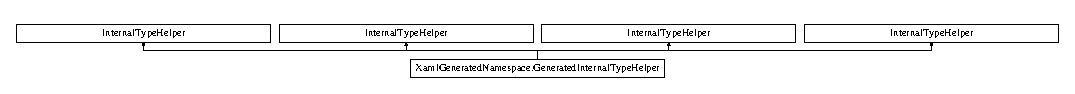
\includegraphics[height=2.000000cm]{class_xaml_generated_namespace_1_1_generated_internal_type_helper}
\end{center}
\end{figure}
\subsection*{Protected Member Functions}
\begin{DoxyCompactItemize}
\item 
override object \hyperlink{class_xaml_generated_namespace_1_1_generated_internal_type_helper_aefb7a98fceb9c287cef4756942f441d1}{Create\+Instance} (System.\+Type type, System.\+Globalization.\+Culture\+Info culture)
\begin{DoxyCompactList}\small\item\em Create\+Instance \end{DoxyCompactList}\item 
override object \hyperlink{class_xaml_generated_namespace_1_1_generated_internal_type_helper_afdc9fe15b56607d02082908d934480c6}{Get\+Property\+Value} (System.\+Reflection.\+Property\+Info property\+Info, object target, System.\+Globalization.\+Culture\+Info culture)
\begin{DoxyCompactList}\small\item\em Get\+Property\+Value \end{DoxyCompactList}\item 
override void \hyperlink{class_xaml_generated_namespace_1_1_generated_internal_type_helper_ade0f04c0f7b18dd5b170e071d5534d38}{Set\+Property\+Value} (System.\+Reflection.\+Property\+Info property\+Info, object target, object value, System.\+Globalization.\+Culture\+Info culture)
\begin{DoxyCompactList}\small\item\em Set\+Property\+Value \end{DoxyCompactList}\item 
override System.\+Delegate \hyperlink{class_xaml_generated_namespace_1_1_generated_internal_type_helper_a8ec4c37e82d9f4e867e9655f4eac3a78}{Create\+Delegate} (System.\+Type delegate\+Type, object target, string handler)
\begin{DoxyCompactList}\small\item\em Create\+Delegate \end{DoxyCompactList}\item 
override void \hyperlink{class_xaml_generated_namespace_1_1_generated_internal_type_helper_a73471f4a6d1ca4c4fceec9ad8610f0c8}{Add\+Event\+Handler} (System.\+Reflection.\+Event\+Info event\+Info, object target, System.\+Delegate handler)
\begin{DoxyCompactList}\small\item\em Add\+Event\+Handler \end{DoxyCompactList}\end{DoxyCompactItemize}


\subsection{Detailed Description}
\hyperlink{class_xaml_generated_namespace_1_1_generated_internal_type_helper}{Generated\+Internal\+Type\+Helper} 



\subsection{Member Function Documentation}
\mbox{\Hypertarget{class_xaml_generated_namespace_1_1_generated_internal_type_helper_a73471f4a6d1ca4c4fceec9ad8610f0c8}\label{class_xaml_generated_namespace_1_1_generated_internal_type_helper_a73471f4a6d1ca4c4fceec9ad8610f0c8}} 
\index{Xaml\+Generated\+Namespace\+::\+Generated\+Internal\+Type\+Helper@{Xaml\+Generated\+Namespace\+::\+Generated\+Internal\+Type\+Helper}!Add\+Event\+Handler@{Add\+Event\+Handler}}
\index{Add\+Event\+Handler@{Add\+Event\+Handler}!Xaml\+Generated\+Namespace\+::\+Generated\+Internal\+Type\+Helper@{Xaml\+Generated\+Namespace\+::\+Generated\+Internal\+Type\+Helper}}
\subsubsection{\texorpdfstring{Add\+Event\+Handler()}{AddEventHandler()}}
{\footnotesize\ttfamily override void Xaml\+Generated\+Namespace.\+Generated\+Internal\+Type\+Helper.\+Add\+Event\+Handler (\begin{DoxyParamCaption}\item[{System.\+Reflection.\+Event\+Info}]{event\+Info,  }\item[{object}]{target,  }\item[{System.\+Delegate}]{handler }\end{DoxyParamCaption})\hspace{0.3cm}{\ttfamily [protected]}}



Add\+Event\+Handler 

\mbox{\Hypertarget{class_xaml_generated_namespace_1_1_generated_internal_type_helper_a8ec4c37e82d9f4e867e9655f4eac3a78}\label{class_xaml_generated_namespace_1_1_generated_internal_type_helper_a8ec4c37e82d9f4e867e9655f4eac3a78}} 
\index{Xaml\+Generated\+Namespace\+::\+Generated\+Internal\+Type\+Helper@{Xaml\+Generated\+Namespace\+::\+Generated\+Internal\+Type\+Helper}!Create\+Delegate@{Create\+Delegate}}
\index{Create\+Delegate@{Create\+Delegate}!Xaml\+Generated\+Namespace\+::\+Generated\+Internal\+Type\+Helper@{Xaml\+Generated\+Namespace\+::\+Generated\+Internal\+Type\+Helper}}
\subsubsection{\texorpdfstring{Create\+Delegate()}{CreateDelegate()}}
{\footnotesize\ttfamily override System.\+Delegate Xaml\+Generated\+Namespace.\+Generated\+Internal\+Type\+Helper.\+Create\+Delegate (\begin{DoxyParamCaption}\item[{System.\+Type}]{delegate\+Type,  }\item[{object}]{target,  }\item[{string}]{handler }\end{DoxyParamCaption})\hspace{0.3cm}{\ttfamily [protected]}}



Create\+Delegate 

\mbox{\Hypertarget{class_xaml_generated_namespace_1_1_generated_internal_type_helper_aefb7a98fceb9c287cef4756942f441d1}\label{class_xaml_generated_namespace_1_1_generated_internal_type_helper_aefb7a98fceb9c287cef4756942f441d1}} 
\index{Xaml\+Generated\+Namespace\+::\+Generated\+Internal\+Type\+Helper@{Xaml\+Generated\+Namespace\+::\+Generated\+Internal\+Type\+Helper}!Create\+Instance@{Create\+Instance}}
\index{Create\+Instance@{Create\+Instance}!Xaml\+Generated\+Namespace\+::\+Generated\+Internal\+Type\+Helper@{Xaml\+Generated\+Namespace\+::\+Generated\+Internal\+Type\+Helper}}
\subsubsection{\texorpdfstring{Create\+Instance()}{CreateInstance()}}
{\footnotesize\ttfamily override object Xaml\+Generated\+Namespace.\+Generated\+Internal\+Type\+Helper.\+Create\+Instance (\begin{DoxyParamCaption}\item[{System.\+Type}]{type,  }\item[{System.\+Globalization.\+Culture\+Info}]{culture }\end{DoxyParamCaption})\hspace{0.3cm}{\ttfamily [protected]}}



Create\+Instance 

\mbox{\Hypertarget{class_xaml_generated_namespace_1_1_generated_internal_type_helper_afdc9fe15b56607d02082908d934480c6}\label{class_xaml_generated_namespace_1_1_generated_internal_type_helper_afdc9fe15b56607d02082908d934480c6}} 
\index{Xaml\+Generated\+Namespace\+::\+Generated\+Internal\+Type\+Helper@{Xaml\+Generated\+Namespace\+::\+Generated\+Internal\+Type\+Helper}!Get\+Property\+Value@{Get\+Property\+Value}}
\index{Get\+Property\+Value@{Get\+Property\+Value}!Xaml\+Generated\+Namespace\+::\+Generated\+Internal\+Type\+Helper@{Xaml\+Generated\+Namespace\+::\+Generated\+Internal\+Type\+Helper}}
\subsubsection{\texorpdfstring{Get\+Property\+Value()}{GetPropertyValue()}}
{\footnotesize\ttfamily override object Xaml\+Generated\+Namespace.\+Generated\+Internal\+Type\+Helper.\+Get\+Property\+Value (\begin{DoxyParamCaption}\item[{System.\+Reflection.\+Property\+Info}]{property\+Info,  }\item[{object}]{target,  }\item[{System.\+Globalization.\+Culture\+Info}]{culture }\end{DoxyParamCaption})\hspace{0.3cm}{\ttfamily [protected]}}



Get\+Property\+Value 

\mbox{\Hypertarget{class_xaml_generated_namespace_1_1_generated_internal_type_helper_ade0f04c0f7b18dd5b170e071d5534d38}\label{class_xaml_generated_namespace_1_1_generated_internal_type_helper_ade0f04c0f7b18dd5b170e071d5534d38}} 
\index{Xaml\+Generated\+Namespace\+::\+Generated\+Internal\+Type\+Helper@{Xaml\+Generated\+Namespace\+::\+Generated\+Internal\+Type\+Helper}!Set\+Property\+Value@{Set\+Property\+Value}}
\index{Set\+Property\+Value@{Set\+Property\+Value}!Xaml\+Generated\+Namespace\+::\+Generated\+Internal\+Type\+Helper@{Xaml\+Generated\+Namespace\+::\+Generated\+Internal\+Type\+Helper}}
\subsubsection{\texorpdfstring{Set\+Property\+Value()}{SetPropertyValue()}}
{\footnotesize\ttfamily override void Xaml\+Generated\+Namespace.\+Generated\+Internal\+Type\+Helper.\+Set\+Property\+Value (\begin{DoxyParamCaption}\item[{System.\+Reflection.\+Property\+Info}]{property\+Info,  }\item[{object}]{target,  }\item[{object}]{value,  }\item[{System.\+Globalization.\+Culture\+Info}]{culture }\end{DoxyParamCaption})\hspace{0.3cm}{\ttfamily [protected]}}



Set\+Property\+Value 



The documentation for this class was generated from the following file\+:\begin{DoxyCompactItemize}
\item 
obj/\+Debug/\hyperlink{_generated_internal_type_helper_8g_8i_8cs}{Generated\+Internal\+Type\+Helper.\+g.\+i.\+cs}\end{DoxyCompactItemize}

\hypertarget{struct_rowing_monitor_1_1_model_1_1_util_1_1_joint_data}{}\section{Rowing\+Monitor.\+Model.\+Util.\+Joint\+Data Struct Reference}
\label{struct_rowing_monitor_1_1_model_1_1_util_1_1_joint_data}\index{Rowing\+Monitor.\+Model.\+Util.\+Joint\+Data@{Rowing\+Monitor.\+Model.\+Util.\+Joint\+Data}}
\subsection*{Properties}
\begin{DoxyCompactItemize}
\item 
double \hyperlink{struct_rowing_monitor_1_1_model_1_1_util_1_1_joint_data_a56463d7bd16c6e5cad4e3619e9df9508}{Rel\+Timestamp}\hspace{0.3cm}{\ttfamily  \mbox{[}get, set\mbox{]}}
\begin{DoxyCompactList}\small\item\em Time in milliseconds since Kinect sensor started. \end{DoxyCompactList}\item 
double \hyperlink{struct_rowing_monitor_1_1_model_1_1_util_1_1_joint_data_a2c951ee40b3e49be73b92cf39c5aa9ab}{Abs\+Timestamp}\hspace{0.3cm}{\ttfamily  \mbox{[}get, set\mbox{]}}
\begin{DoxyCompactList}\small\item\em Time in milliseconds since first frame. \end{DoxyCompactList}\item 
I\+Read\+Only\+Dictionary$<$ Joint\+Type, Joint $>$ \hyperlink{struct_rowing_monitor_1_1_model_1_1_util_1_1_joint_data_afa67f920730db9679102686913774e69}{Joints}\hspace{0.3cm}{\ttfamily  \mbox{[}get, set\mbox{]}}
\begin{DoxyCompactList}\small\item\em Positions of all joints. \end{DoxyCompactList}\item 
long \hyperlink{struct_rowing_monitor_1_1_model_1_1_util_1_1_joint_data_a2193c6359b3e9e2d6dfdb6178351a8b3}{Index}\hspace{0.3cm}{\ttfamily  \mbox{[}get, set\mbox{]}}
\begin{DoxyCompactList}\small\item\em Incrementing number of frames. \end{DoxyCompactList}\item 
List$<$ double $>$ \hyperlink{struct_rowing_monitor_1_1_model_1_1_util_1_1_joint_data_a98bf571ea92c7f9b8e197062f17ddc27}{Timestamps}\hspace{0.3cm}{\ttfamily  \mbox{[}get, set\mbox{]}}
\begin{DoxyCompactList}\small\item\em List of all timestamps that were set in the pipeline \end{DoxyCompactList}\item 
\hyperlink{namespace_rowing_monitor_1_1_model_1_1_util_a01e1a06061533b246feb7421c9d0107f}{Data\+Stream\+Type} \hyperlink{struct_rowing_monitor_1_1_model_1_1_util_1_1_joint_data_a8ed0022c598484f0b418ad30b50bbfb6}{Data\+Stream\+Type}\hspace{0.3cm}{\ttfamily  \mbox{[}get, set\mbox{]}}
\begin{DoxyCompactList}\small\item\em Type of the data. \end{DoxyCompactList}\item 
bool \hyperlink{struct_rowing_monitor_1_1_model_1_1_util_1_1_joint_data_a1e86bf9206df62d0fb4b77c8017ccf8a}{Is\+Empty}\hspace{0.3cm}{\ttfamily  \mbox{[}get\mbox{]}}
\begin{DoxyCompactList}\small\item\em Returns true if this element conatins no joint data. \end{DoxyCompactList}\end{DoxyCompactItemize}


\subsection{Property Documentation}
\mbox{\Hypertarget{struct_rowing_monitor_1_1_model_1_1_util_1_1_joint_data_a2c951ee40b3e49be73b92cf39c5aa9ab}\label{struct_rowing_monitor_1_1_model_1_1_util_1_1_joint_data_a2c951ee40b3e49be73b92cf39c5aa9ab}} 
\index{Rowing\+Monitor\+::\+Model\+::\+Util\+::\+Joint\+Data@{Rowing\+Monitor\+::\+Model\+::\+Util\+::\+Joint\+Data}!Abs\+Timestamp@{Abs\+Timestamp}}
\index{Abs\+Timestamp@{Abs\+Timestamp}!Rowing\+Monitor\+::\+Model\+::\+Util\+::\+Joint\+Data@{Rowing\+Monitor\+::\+Model\+::\+Util\+::\+Joint\+Data}}
\subsubsection{\texorpdfstring{Abs\+Timestamp}{AbsTimestamp}}
{\footnotesize\ttfamily double Rowing\+Monitor.\+Model.\+Util.\+Joint\+Data.\+Abs\+Timestamp\hspace{0.3cm}{\ttfamily [get]}, {\ttfamily [set]}}



Time in milliseconds since first frame. 

\mbox{\Hypertarget{struct_rowing_monitor_1_1_model_1_1_util_1_1_joint_data_a8ed0022c598484f0b418ad30b50bbfb6}\label{struct_rowing_monitor_1_1_model_1_1_util_1_1_joint_data_a8ed0022c598484f0b418ad30b50bbfb6}} 
\index{Rowing\+Monitor\+::\+Model\+::\+Util\+::\+Joint\+Data@{Rowing\+Monitor\+::\+Model\+::\+Util\+::\+Joint\+Data}!Data\+Stream\+Type@{Data\+Stream\+Type}}
\index{Data\+Stream\+Type@{Data\+Stream\+Type}!Rowing\+Monitor\+::\+Model\+::\+Util\+::\+Joint\+Data@{Rowing\+Monitor\+::\+Model\+::\+Util\+::\+Joint\+Data}}
\subsubsection{\texorpdfstring{Data\+Stream\+Type}{DataStreamType}}
{\footnotesize\ttfamily \hyperlink{namespace_rowing_monitor_1_1_model_1_1_util_a01e1a06061533b246feb7421c9d0107f}{Data\+Stream\+Type} Rowing\+Monitor.\+Model.\+Util.\+Joint\+Data.\+Data\+Stream\+Type\hspace{0.3cm}{\ttfamily [get]}, {\ttfamily [set]}}



Type of the data. 

\mbox{\Hypertarget{struct_rowing_monitor_1_1_model_1_1_util_1_1_joint_data_a2193c6359b3e9e2d6dfdb6178351a8b3}\label{struct_rowing_monitor_1_1_model_1_1_util_1_1_joint_data_a2193c6359b3e9e2d6dfdb6178351a8b3}} 
\index{Rowing\+Monitor\+::\+Model\+::\+Util\+::\+Joint\+Data@{Rowing\+Monitor\+::\+Model\+::\+Util\+::\+Joint\+Data}!Index@{Index}}
\index{Index@{Index}!Rowing\+Monitor\+::\+Model\+::\+Util\+::\+Joint\+Data@{Rowing\+Monitor\+::\+Model\+::\+Util\+::\+Joint\+Data}}
\subsubsection{\texorpdfstring{Index}{Index}}
{\footnotesize\ttfamily long Rowing\+Monitor.\+Model.\+Util.\+Joint\+Data.\+Index\hspace{0.3cm}{\ttfamily [get]}, {\ttfamily [set]}}



Incrementing number of frames. 

\mbox{\Hypertarget{struct_rowing_monitor_1_1_model_1_1_util_1_1_joint_data_a1e86bf9206df62d0fb4b77c8017ccf8a}\label{struct_rowing_monitor_1_1_model_1_1_util_1_1_joint_data_a1e86bf9206df62d0fb4b77c8017ccf8a}} 
\index{Rowing\+Monitor\+::\+Model\+::\+Util\+::\+Joint\+Data@{Rowing\+Monitor\+::\+Model\+::\+Util\+::\+Joint\+Data}!Is\+Empty@{Is\+Empty}}
\index{Is\+Empty@{Is\+Empty}!Rowing\+Monitor\+::\+Model\+::\+Util\+::\+Joint\+Data@{Rowing\+Monitor\+::\+Model\+::\+Util\+::\+Joint\+Data}}
\subsubsection{\texorpdfstring{Is\+Empty}{IsEmpty}}
{\footnotesize\ttfamily bool Rowing\+Monitor.\+Model.\+Util.\+Joint\+Data.\+Is\+Empty\hspace{0.3cm}{\ttfamily [get]}}



Returns true if this element conatins no joint data. 

\mbox{\Hypertarget{struct_rowing_monitor_1_1_model_1_1_util_1_1_joint_data_afa67f920730db9679102686913774e69}\label{struct_rowing_monitor_1_1_model_1_1_util_1_1_joint_data_afa67f920730db9679102686913774e69}} 
\index{Rowing\+Monitor\+::\+Model\+::\+Util\+::\+Joint\+Data@{Rowing\+Monitor\+::\+Model\+::\+Util\+::\+Joint\+Data}!Joints@{Joints}}
\index{Joints@{Joints}!Rowing\+Monitor\+::\+Model\+::\+Util\+::\+Joint\+Data@{Rowing\+Monitor\+::\+Model\+::\+Util\+::\+Joint\+Data}}
\subsubsection{\texorpdfstring{Joints}{Joints}}
{\footnotesize\ttfamily I\+Read\+Only\+Dictionary$<$Joint\+Type, Joint$>$ Rowing\+Monitor.\+Model.\+Util.\+Joint\+Data.\+Joints\hspace{0.3cm}{\ttfamily [get]}, {\ttfamily [set]}}



Positions of all joints. 

\mbox{\Hypertarget{struct_rowing_monitor_1_1_model_1_1_util_1_1_joint_data_a56463d7bd16c6e5cad4e3619e9df9508}\label{struct_rowing_monitor_1_1_model_1_1_util_1_1_joint_data_a56463d7bd16c6e5cad4e3619e9df9508}} 
\index{Rowing\+Monitor\+::\+Model\+::\+Util\+::\+Joint\+Data@{Rowing\+Monitor\+::\+Model\+::\+Util\+::\+Joint\+Data}!Rel\+Timestamp@{Rel\+Timestamp}}
\index{Rel\+Timestamp@{Rel\+Timestamp}!Rowing\+Monitor\+::\+Model\+::\+Util\+::\+Joint\+Data@{Rowing\+Monitor\+::\+Model\+::\+Util\+::\+Joint\+Data}}
\subsubsection{\texorpdfstring{Rel\+Timestamp}{RelTimestamp}}
{\footnotesize\ttfamily double Rowing\+Monitor.\+Model.\+Util.\+Joint\+Data.\+Rel\+Timestamp\hspace{0.3cm}{\ttfamily [get]}, {\ttfamily [set]}}



Time in milliseconds since Kinect sensor started. 

\mbox{\Hypertarget{struct_rowing_monitor_1_1_model_1_1_util_1_1_joint_data_a98bf571ea92c7f9b8e197062f17ddc27}\label{struct_rowing_monitor_1_1_model_1_1_util_1_1_joint_data_a98bf571ea92c7f9b8e197062f17ddc27}} 
\index{Rowing\+Monitor\+::\+Model\+::\+Util\+::\+Joint\+Data@{Rowing\+Monitor\+::\+Model\+::\+Util\+::\+Joint\+Data}!Timestamps@{Timestamps}}
\index{Timestamps@{Timestamps}!Rowing\+Monitor\+::\+Model\+::\+Util\+::\+Joint\+Data@{Rowing\+Monitor\+::\+Model\+::\+Util\+::\+Joint\+Data}}
\subsubsection{\texorpdfstring{Timestamps}{Timestamps}}
{\footnotesize\ttfamily List$<$double$>$ Rowing\+Monitor.\+Model.\+Util.\+Joint\+Data.\+Timestamps\hspace{0.3cm}{\ttfamily [get]}, {\ttfamily [set]}}



List of all timestamps that were set in the pipeline 



The documentation for this struct was generated from the following file\+:\begin{DoxyCompactItemize}
\item 
Model/\+Util/\hyperlink{_joint_data_handler_8cs}{Joint\+Data\+Handler.\+cs}\end{DoxyCompactItemize}

\hypertarget{class_rowing_monitor_1_1_model_1_1_util_1_1_kinect_data_handler}{}\section{Rowing\+Monitor.\+Model.\+Util.\+Kinect\+Data\+Handler Class Reference}
\label{class_rowing_monitor_1_1_model_1_1_util_1_1_kinect_data_handler}\index{Rowing\+Monitor.\+Model.\+Util.\+Kinect\+Data\+Handler@{Rowing\+Monitor.\+Model.\+Util.\+Kinect\+Data\+Handler}}
\subsection*{Public Member Functions}
\begin{DoxyCompactItemize}
\item 
\hyperlink{struct_rowing_monitor_1_1_model_1_1_util_1_1_joint_data}{Joint\+Data} \hyperlink{class_rowing_monitor_1_1_model_1_1_util_1_1_kinect_data_handler_aad695db8966d25a7c4226c369bc6be32}{Create\+New\+Joint\+Data} (double rel\+Timestamp, double creation\+Timestamp, I\+Read\+Only\+Dictionary$<$ Joint\+Type, Joint $>$ joints)
\item 
Body \hyperlink{class_rowing_monitor_1_1_model_1_1_util_1_1_kinect_data_handler_a51dce526e2a10d64012371da702ab519}{Get\+First\+Tracked\+Body} ()
\begin{DoxyCompactList}\small\item\em Return the longest tracked body. \end{DoxyCompactList}\end{DoxyCompactItemize}
\subsection*{Static Public Member Functions}
\begin{DoxyCompactItemize}
\item 
static \hyperlink{struct_rowing_monitor_1_1_model_1_1_util_1_1_joint_data}{Joint\+Data} \hyperlink{class_rowing_monitor_1_1_model_1_1_util_1_1_kinect_data_handler_aa3deffa0d869598352bff14c43dc3a7b}{Replace\+Joints\+In\+Joint\+Data} (\hyperlink{struct_rowing_monitor_1_1_model_1_1_util_1_1_joint_data}{Joint\+Data} old\+Joint\+Data, double creation\+Timestamp, I\+Read\+Only\+Dictionary$<$ Joint\+Type, Joint $>$ new\+Joints)
\end{DoxyCompactItemize}
\subsection*{Properties}
\begin{DoxyCompactItemize}
\item 
static \hyperlink{class_rowing_monitor_1_1_model_1_1_util_1_1_kinect_data_handler}{Kinect\+Data\+Handler} \hyperlink{class_rowing_monitor_1_1_model_1_1_util_1_1_kinect_data_handler_ad9209193c7b73ab88e4398bfa9c2d0b2}{Instance}\hspace{0.3cm}{\ttfamily  \mbox{[}get\mbox{]}}
\item 
double \hyperlink{class_rowing_monitor_1_1_model_1_1_util_1_1_kinect_data_handler_aa21aa573d216387e67181b49bf4eb4f5}{Rel\+Start\+Time}\hspace{0.3cm}{\ttfamily  \mbox{[}get, set\mbox{]}}
\item 
long \hyperlink{class_rowing_monitor_1_1_model_1_1_util_1_1_kinect_data_handler_abd75c2380b775c7d858e681249e3685c}{Last\+Index}\hspace{0.3cm}{\ttfamily  \mbox{[}get, set\mbox{]}}
\item 
Body \mbox{[}$\,$\mbox{]} \hyperlink{class_rowing_monitor_1_1_model_1_1_util_1_1_kinect_data_handler_a099b9bc04fc8023717be35549aaeddda}{Bodies}\hspace{0.3cm}{\ttfamily  \mbox{[}get, set\mbox{]}}
\end{DoxyCompactItemize}


\subsection{Member Function Documentation}
\mbox{\Hypertarget{class_rowing_monitor_1_1_model_1_1_util_1_1_kinect_data_handler_aad695db8966d25a7c4226c369bc6be32}\label{class_rowing_monitor_1_1_model_1_1_util_1_1_kinect_data_handler_aad695db8966d25a7c4226c369bc6be32}} 
\index{Rowing\+Monitor\+::\+Model\+::\+Util\+::\+Kinect\+Data\+Handler@{Rowing\+Monitor\+::\+Model\+::\+Util\+::\+Kinect\+Data\+Handler}!Create\+New\+Joint\+Data@{Create\+New\+Joint\+Data}}
\index{Create\+New\+Joint\+Data@{Create\+New\+Joint\+Data}!Rowing\+Monitor\+::\+Model\+::\+Util\+::\+Kinect\+Data\+Handler@{Rowing\+Monitor\+::\+Model\+::\+Util\+::\+Kinect\+Data\+Handler}}
\subsubsection{\texorpdfstring{Create\+New\+Joint\+Data()}{CreateNewJointData()}}
{\footnotesize\ttfamily \hyperlink{struct_rowing_monitor_1_1_model_1_1_util_1_1_joint_data}{Joint\+Data} Rowing\+Monitor.\+Model.\+Util.\+Kinect\+Data\+Handler.\+Create\+New\+Joint\+Data (\begin{DoxyParamCaption}\item[{double}]{rel\+Timestamp,  }\item[{double}]{creation\+Timestamp,  }\item[{I\+Read\+Only\+Dictionary$<$ Joint\+Type, Joint $>$}]{joints }\end{DoxyParamCaption})}

\mbox{\Hypertarget{class_rowing_monitor_1_1_model_1_1_util_1_1_kinect_data_handler_a51dce526e2a10d64012371da702ab519}\label{class_rowing_monitor_1_1_model_1_1_util_1_1_kinect_data_handler_a51dce526e2a10d64012371da702ab519}} 
\index{Rowing\+Monitor\+::\+Model\+::\+Util\+::\+Kinect\+Data\+Handler@{Rowing\+Monitor\+::\+Model\+::\+Util\+::\+Kinect\+Data\+Handler}!Get\+First\+Tracked\+Body@{Get\+First\+Tracked\+Body}}
\index{Get\+First\+Tracked\+Body@{Get\+First\+Tracked\+Body}!Rowing\+Monitor\+::\+Model\+::\+Util\+::\+Kinect\+Data\+Handler@{Rowing\+Monitor\+::\+Model\+::\+Util\+::\+Kinect\+Data\+Handler}}
\subsubsection{\texorpdfstring{Get\+First\+Tracked\+Body()}{GetFirstTrackedBody()}}
{\footnotesize\ttfamily Body Rowing\+Monitor.\+Model.\+Util.\+Kinect\+Data\+Handler.\+Get\+First\+Tracked\+Body (\begin{DoxyParamCaption}{ }\end{DoxyParamCaption})}



Return the longest tracked body. 

\begin{DoxyReturn}{Returns}

\end{DoxyReturn}
\mbox{\Hypertarget{class_rowing_monitor_1_1_model_1_1_util_1_1_kinect_data_handler_aa3deffa0d869598352bff14c43dc3a7b}\label{class_rowing_monitor_1_1_model_1_1_util_1_1_kinect_data_handler_aa3deffa0d869598352bff14c43dc3a7b}} 
\index{Rowing\+Monitor\+::\+Model\+::\+Util\+::\+Kinect\+Data\+Handler@{Rowing\+Monitor\+::\+Model\+::\+Util\+::\+Kinect\+Data\+Handler}!Replace\+Joints\+In\+Joint\+Data@{Replace\+Joints\+In\+Joint\+Data}}
\index{Replace\+Joints\+In\+Joint\+Data@{Replace\+Joints\+In\+Joint\+Data}!Rowing\+Monitor\+::\+Model\+::\+Util\+::\+Kinect\+Data\+Handler@{Rowing\+Monitor\+::\+Model\+::\+Util\+::\+Kinect\+Data\+Handler}}
\subsubsection{\texorpdfstring{Replace\+Joints\+In\+Joint\+Data()}{ReplaceJointsInJointData()}}
{\footnotesize\ttfamily static \hyperlink{struct_rowing_monitor_1_1_model_1_1_util_1_1_joint_data}{Joint\+Data} Rowing\+Monitor.\+Model.\+Util.\+Kinect\+Data\+Handler.\+Replace\+Joints\+In\+Joint\+Data (\begin{DoxyParamCaption}\item[{\hyperlink{struct_rowing_monitor_1_1_model_1_1_util_1_1_joint_data}{Joint\+Data}}]{old\+Joint\+Data,  }\item[{double}]{creation\+Timestamp,  }\item[{I\+Read\+Only\+Dictionary$<$ Joint\+Type, Joint $>$}]{new\+Joints }\end{DoxyParamCaption})\hspace{0.3cm}{\ttfamily [static]}}



\subsection{Property Documentation}
\mbox{\Hypertarget{class_rowing_monitor_1_1_model_1_1_util_1_1_kinect_data_handler_a099b9bc04fc8023717be35549aaeddda}\label{class_rowing_monitor_1_1_model_1_1_util_1_1_kinect_data_handler_a099b9bc04fc8023717be35549aaeddda}} 
\index{Rowing\+Monitor\+::\+Model\+::\+Util\+::\+Kinect\+Data\+Handler@{Rowing\+Monitor\+::\+Model\+::\+Util\+::\+Kinect\+Data\+Handler}!Bodies@{Bodies}}
\index{Bodies@{Bodies}!Rowing\+Monitor\+::\+Model\+::\+Util\+::\+Kinect\+Data\+Handler@{Rowing\+Monitor\+::\+Model\+::\+Util\+::\+Kinect\+Data\+Handler}}
\subsubsection{\texorpdfstring{Bodies}{Bodies}}
{\footnotesize\ttfamily Body \mbox{[}$\,$\mbox{]} Rowing\+Monitor.\+Model.\+Util.\+Kinect\+Data\+Handler.\+Bodies\hspace{0.3cm}{\ttfamily [get]}, {\ttfamily [set]}}

\mbox{\Hypertarget{class_rowing_monitor_1_1_model_1_1_util_1_1_kinect_data_handler_ad9209193c7b73ab88e4398bfa9c2d0b2}\label{class_rowing_monitor_1_1_model_1_1_util_1_1_kinect_data_handler_ad9209193c7b73ab88e4398bfa9c2d0b2}} 
\index{Rowing\+Monitor\+::\+Model\+::\+Util\+::\+Kinect\+Data\+Handler@{Rowing\+Monitor\+::\+Model\+::\+Util\+::\+Kinect\+Data\+Handler}!Instance@{Instance}}
\index{Instance@{Instance}!Rowing\+Monitor\+::\+Model\+::\+Util\+::\+Kinect\+Data\+Handler@{Rowing\+Monitor\+::\+Model\+::\+Util\+::\+Kinect\+Data\+Handler}}
\subsubsection{\texorpdfstring{Instance}{Instance}}
{\footnotesize\ttfamily \hyperlink{class_rowing_monitor_1_1_model_1_1_util_1_1_kinect_data_handler}{Kinect\+Data\+Handler} Rowing\+Monitor.\+Model.\+Util.\+Kinect\+Data\+Handler.\+Instance\hspace{0.3cm}{\ttfamily [static]}, {\ttfamily [get]}}

\mbox{\Hypertarget{class_rowing_monitor_1_1_model_1_1_util_1_1_kinect_data_handler_abd75c2380b775c7d858e681249e3685c}\label{class_rowing_monitor_1_1_model_1_1_util_1_1_kinect_data_handler_abd75c2380b775c7d858e681249e3685c}} 
\index{Rowing\+Monitor\+::\+Model\+::\+Util\+::\+Kinect\+Data\+Handler@{Rowing\+Monitor\+::\+Model\+::\+Util\+::\+Kinect\+Data\+Handler}!Last\+Index@{Last\+Index}}
\index{Last\+Index@{Last\+Index}!Rowing\+Monitor\+::\+Model\+::\+Util\+::\+Kinect\+Data\+Handler@{Rowing\+Monitor\+::\+Model\+::\+Util\+::\+Kinect\+Data\+Handler}}
\subsubsection{\texorpdfstring{Last\+Index}{LastIndex}}
{\footnotesize\ttfamily long Rowing\+Monitor.\+Model.\+Util.\+Kinect\+Data\+Handler.\+Last\+Index\hspace{0.3cm}{\ttfamily [get]}, {\ttfamily [set]}}

\mbox{\Hypertarget{class_rowing_monitor_1_1_model_1_1_util_1_1_kinect_data_handler_aa21aa573d216387e67181b49bf4eb4f5}\label{class_rowing_monitor_1_1_model_1_1_util_1_1_kinect_data_handler_aa21aa573d216387e67181b49bf4eb4f5}} 
\index{Rowing\+Monitor\+::\+Model\+::\+Util\+::\+Kinect\+Data\+Handler@{Rowing\+Monitor\+::\+Model\+::\+Util\+::\+Kinect\+Data\+Handler}!Rel\+Start\+Time@{Rel\+Start\+Time}}
\index{Rel\+Start\+Time@{Rel\+Start\+Time}!Rowing\+Monitor\+::\+Model\+::\+Util\+::\+Kinect\+Data\+Handler@{Rowing\+Monitor\+::\+Model\+::\+Util\+::\+Kinect\+Data\+Handler}}
\subsubsection{\texorpdfstring{Rel\+Start\+Time}{RelStartTime}}
{\footnotesize\ttfamily double Rowing\+Monitor.\+Model.\+Util.\+Kinect\+Data\+Handler.\+Rel\+Start\+Time\hspace{0.3cm}{\ttfamily [get]}, {\ttfamily [set]}}



The documentation for this class was generated from the following file\+:\begin{DoxyCompactItemize}
\item 
Model/\+Util/\hyperlink{_kinect_data_handler_8cs}{Kinect\+Data\+Handler.\+cs}\end{DoxyCompactItemize}

\hypertarget{class_rowing_monitor_1_1_model_1_1_kinect_frame_arrived_event_args}{}\section{Rowing\+Monitor.\+Model.\+Kinect\+Frame\+Arrived\+Event\+Args Class Reference}
\label{class_rowing_monitor_1_1_model_1_1_kinect_frame_arrived_event_args}\index{Rowing\+Monitor.\+Model.\+Kinect\+Frame\+Arrived\+Event\+Args@{Rowing\+Monitor.\+Model.\+Kinect\+Frame\+Arrived\+Event\+Args}}


Represents the arguments for a Kinect\+Reader\textquotesingle{}s Frame\+Arrived event.  


Inheritance diagram for Rowing\+Monitor.\+Model.\+Kinect\+Frame\+Arrived\+Event\+Args\+:\begin{figure}[H]
\begin{center}
\leavevmode
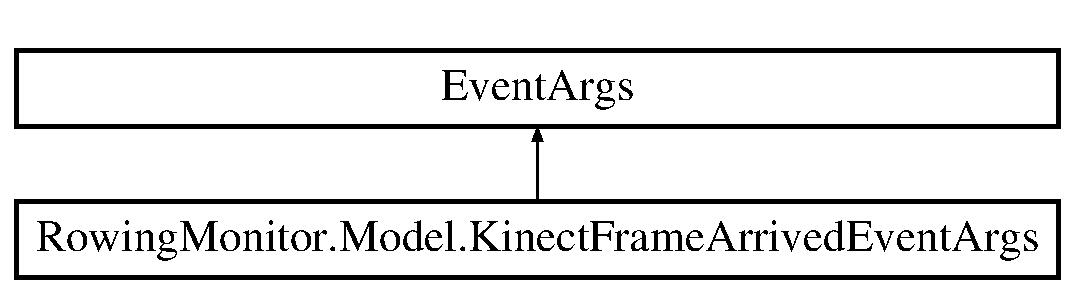
\includegraphics[height=2.000000cm]{class_rowing_monitor_1_1_model_1_1_kinect_frame_arrived_event_args}
\end{center}
\end{figure}
\subsection*{Public Member Functions}
\begin{DoxyCompactItemize}
\item 
\hyperlink{class_rowing_monitor_1_1_model_1_1_kinect_frame_arrived_event_args_a6c0155b21bc19c9fe163c5ea9ef66b21}{Kinect\+Frame\+Arrived\+Event\+Args} (\hyperlink{struct_rowing_monitor_1_1_model_1_1_util_1_1_joint_data}{Joint\+Data} joint\+Data)
\end{DoxyCompactItemize}
\subsection*{Properties}
\begin{DoxyCompactItemize}
\item 
\hyperlink{struct_rowing_monitor_1_1_model_1_1_util_1_1_joint_data}{Joint\+Data} \hyperlink{class_rowing_monitor_1_1_model_1_1_kinect_frame_arrived_event_args_a2249c19be25bb9b2c3627fb1bfa7512b}{Joint\+Data}\hspace{0.3cm}{\ttfamily  \mbox{[}get\mbox{]}}
\end{DoxyCompactItemize}


\subsection{Detailed Description}
Represents the arguments for a Kinect\+Reader\textquotesingle{}s Frame\+Arrived event. 



\subsection{Constructor \& Destructor Documentation}
\mbox{\Hypertarget{class_rowing_monitor_1_1_model_1_1_kinect_frame_arrived_event_args_a6c0155b21bc19c9fe163c5ea9ef66b21}\label{class_rowing_monitor_1_1_model_1_1_kinect_frame_arrived_event_args_a6c0155b21bc19c9fe163c5ea9ef66b21}} 
\index{Rowing\+Monitor\+::\+Model\+::\+Kinect\+Frame\+Arrived\+Event\+Args@{Rowing\+Monitor\+::\+Model\+::\+Kinect\+Frame\+Arrived\+Event\+Args}!Kinect\+Frame\+Arrived\+Event\+Args@{Kinect\+Frame\+Arrived\+Event\+Args}}
\index{Kinect\+Frame\+Arrived\+Event\+Args@{Kinect\+Frame\+Arrived\+Event\+Args}!Rowing\+Monitor\+::\+Model\+::\+Kinect\+Frame\+Arrived\+Event\+Args@{Rowing\+Monitor\+::\+Model\+::\+Kinect\+Frame\+Arrived\+Event\+Args}}
\subsubsection{\texorpdfstring{Kinect\+Frame\+Arrived\+Event\+Args()}{KinectFrameArrivedEventArgs()}}
{\footnotesize\ttfamily Rowing\+Monitor.\+Model.\+Kinect\+Frame\+Arrived\+Event\+Args.\+Kinect\+Frame\+Arrived\+Event\+Args (\begin{DoxyParamCaption}\item[{\hyperlink{struct_rowing_monitor_1_1_model_1_1_util_1_1_joint_data}{Joint\+Data}}]{joint\+Data }\end{DoxyParamCaption})}



\subsection{Property Documentation}
\mbox{\Hypertarget{class_rowing_monitor_1_1_model_1_1_kinect_frame_arrived_event_args_a2249c19be25bb9b2c3627fb1bfa7512b}\label{class_rowing_monitor_1_1_model_1_1_kinect_frame_arrived_event_args_a2249c19be25bb9b2c3627fb1bfa7512b}} 
\index{Rowing\+Monitor\+::\+Model\+::\+Kinect\+Frame\+Arrived\+Event\+Args@{Rowing\+Monitor\+::\+Model\+::\+Kinect\+Frame\+Arrived\+Event\+Args}!Joint\+Data@{Joint\+Data}}
\index{Joint\+Data@{Joint\+Data}!Rowing\+Monitor\+::\+Model\+::\+Kinect\+Frame\+Arrived\+Event\+Args@{Rowing\+Monitor\+::\+Model\+::\+Kinect\+Frame\+Arrived\+Event\+Args}}
\subsubsection{\texorpdfstring{Joint\+Data}{JointData}}
{\footnotesize\ttfamily \hyperlink{struct_rowing_monitor_1_1_model_1_1_util_1_1_joint_data}{Joint\+Data} Rowing\+Monitor.\+Model.\+Kinect\+Frame\+Arrived\+Event\+Args.\+Joint\+Data\hspace{0.3cm}{\ttfamily [get]}}



The documentation for this class was generated from the following file\+:\begin{DoxyCompactItemize}
\item 
Model/\+Event\+Args/\hyperlink{_kinect_frame_arrived_event_args_8cs}{Kinect\+Frame\+Arrived\+Event\+Args.\+cs}\end{DoxyCompactItemize}

\hypertarget{class_rowing_monitor_1_1_model_1_1_pipeline_1_1_kinect_joint_filter}{}\section{Rowing\+Monitor.\+Model.\+Pipeline.\+Kinect\+Joint\+Filter Class Reference}
\label{class_rowing_monitor_1_1_model_1_1_pipeline_1_1_kinect_joint_filter}\index{Rowing\+Monitor.\+Model.\+Pipeline.\+Kinect\+Joint\+Filter@{Rowing\+Monitor.\+Model.\+Pipeline.\+Kinect\+Joint\+Filter}}


Adapted default Kinect smoothing filter to work with the pipeline. \href{https://social.msdn.microsoft.com/Forums/en-US/ffbc8ec7-7551-4462-88aa-2fab69eac38f/joint-smoothing-code-c-errors-in-kinectjointfilter-class?forum=kinectv2sdk}{\tt https\+://social.\+msdn.\+microsoft.\+com/\+Forums/en-\/\+U\+S/ffbc8ec7-\/7551-\/4462-\/88aa-\/2fab69eac38f/joint-\/smoothing-\/code-\/c-\/errors-\/in-\/kinectjointfilter-\/class?forum=kinectv2sdk}  


\subsection*{Classes}
\begin{DoxyCompactItemize}
\item 
class \hyperlink{class_rowing_monitor_1_1_model_1_1_pipeline_1_1_kinect_joint_filter_1_1_filter_double_exponential_data}{Filter\+Double\+Exponential\+Data}
\item 
struct \hyperlink{struct_rowing_monitor_1_1_model_1_1_pipeline_1_1_kinect_joint_filter_1_1_t_r_a_n_s_f_o_r_m___s_m_o_o_t_h___p_a_r_a_m_e_t_e_r_s}{T\+R\+A\+N\+S\+F\+O\+R\+M\+\_\+\+S\+M\+O\+O\+T\+H\+\_\+\+P\+A\+R\+A\+M\+E\+T\+E\+RS}
\end{DoxyCompactItemize}
\subsection*{Public Member Functions}
\begin{DoxyCompactItemize}
\item 
delegate void \hyperlink{class_rowing_monitor_1_1_model_1_1_pipeline_1_1_kinect_joint_filter_ac3f380b74d953666c314d93452c3e1f5}{Smoothed\+Frame\+Arrived\+Event\+Handler} (Object sender, \hyperlink{class_rowing_monitor_1_1_model_1_1_smoothed_frame_arrived_event_args}{Smoothed\+Frame\+Arrived\+Event\+Args} e)
\item 
\hyperlink{class_rowing_monitor_1_1_model_1_1_pipeline_1_1_kinect_joint_filter_a9da91926de15721cdc7631b6c9966ab7}{Kinect\+Joint\+Filter} ()
\item 
void \hyperlink{class_rowing_monitor_1_1_model_1_1_pipeline_1_1_kinect_joint_filter_ad057ad56f551f53d46e8b3b8ce11f1aa}{Init} (float f\+Smoothing=0.\+25f, float f\+Correction=0.\+25f, float f\+Prediction=0.\+25f, float f\+Jitter\+Radius=0.\+03f, float f\+Max\+Deviation\+Radius=0.\+05f)
\item 
void \hyperlink{class_rowing_monitor_1_1_model_1_1_pipeline_1_1_kinect_joint_filter_a7fa54bbd5a70ae429a3faac8e732daf1}{Shutdown} ()
\item 
void \hyperlink{class_rowing_monitor_1_1_model_1_1_pipeline_1_1_kinect_joint_filter_a1ae0e8f5936e1c6a4294a0db5e360996}{Reset} (float f\+Smoothing=0.\+25f, float f\+Correction=0.\+25f, float f\+Prediction=0.\+25f, float f\+Jitter\+Radius=0.\+03f, float f\+Max\+Deviation\+Radius=0.\+05f)
\item 
void \hyperlink{class_rowing_monitor_1_1_model_1_1_pipeline_1_1_kinect_joint_filter_a93d08940ef6304498c4ff9ad6262c266}{Update\+Filter} (\hyperlink{struct_rowing_monitor_1_1_model_1_1_util_1_1_joint_data}{Joint\+Data} joint\+Data)
\item 
Camera\+Space\+Point \mbox{[}$\,$\mbox{]} \hyperlink{class_rowing_monitor_1_1_model_1_1_pipeline_1_1_kinect_joint_filter_afacadd63a8975388f5b40346c6a7579e}{Get\+Filtered\+Joints} ()
\end{DoxyCompactItemize}
\subsection*{Events}
\begin{DoxyCompactItemize}
\item 
\hyperlink{class_rowing_monitor_1_1_model_1_1_pipeline_1_1_kinect_joint_filter_ac3f380b74d953666c314d93452c3e1f5}{Smoothed\+Frame\+Arrived\+Event\+Handler} \hyperlink{class_rowing_monitor_1_1_model_1_1_pipeline_1_1_kinect_joint_filter_a277ea9127efcee74bd306b85103034f7}{Smoothed\+Frame\+Arrived}
\end{DoxyCompactItemize}


\subsection{Detailed Description}
Adapted default Kinect smoothing filter to work with the pipeline. \href{https://social.msdn.microsoft.com/Forums/en-US/ffbc8ec7-7551-4462-88aa-2fab69eac38f/joint-smoothing-code-c-errors-in-kinectjointfilter-class?forum=kinectv2sdk}{\tt https\+://social.\+msdn.\+microsoft.\+com/\+Forums/en-\/\+U\+S/ffbc8ec7-\/7551-\/4462-\/88aa-\/2fab69eac38f/joint-\/smoothing-\/code-\/c-\/errors-\/in-\/kinectjointfilter-\/class?forum=kinectv2sdk} 



\subsection{Constructor \& Destructor Documentation}
\mbox{\Hypertarget{class_rowing_monitor_1_1_model_1_1_pipeline_1_1_kinect_joint_filter_a9da91926de15721cdc7631b6c9966ab7}\label{class_rowing_monitor_1_1_model_1_1_pipeline_1_1_kinect_joint_filter_a9da91926de15721cdc7631b6c9966ab7}} 
\index{Rowing\+Monitor\+::\+Model\+::\+Pipeline\+::\+Kinect\+Joint\+Filter@{Rowing\+Monitor\+::\+Model\+::\+Pipeline\+::\+Kinect\+Joint\+Filter}!Kinect\+Joint\+Filter@{Kinect\+Joint\+Filter}}
\index{Kinect\+Joint\+Filter@{Kinect\+Joint\+Filter}!Rowing\+Monitor\+::\+Model\+::\+Pipeline\+::\+Kinect\+Joint\+Filter@{Rowing\+Monitor\+::\+Model\+::\+Pipeline\+::\+Kinect\+Joint\+Filter}}
\subsubsection{\texorpdfstring{Kinect\+Joint\+Filter()}{KinectJointFilter()}}
{\footnotesize\ttfamily Rowing\+Monitor.\+Model.\+Pipeline.\+Kinect\+Joint\+Filter.\+Kinect\+Joint\+Filter (\begin{DoxyParamCaption}{ }\end{DoxyParamCaption})}



\subsection{Member Function Documentation}
\mbox{\Hypertarget{class_rowing_monitor_1_1_model_1_1_pipeline_1_1_kinect_joint_filter_afacadd63a8975388f5b40346c6a7579e}\label{class_rowing_monitor_1_1_model_1_1_pipeline_1_1_kinect_joint_filter_afacadd63a8975388f5b40346c6a7579e}} 
\index{Rowing\+Monitor\+::\+Model\+::\+Pipeline\+::\+Kinect\+Joint\+Filter@{Rowing\+Monitor\+::\+Model\+::\+Pipeline\+::\+Kinect\+Joint\+Filter}!Get\+Filtered\+Joints@{Get\+Filtered\+Joints}}
\index{Get\+Filtered\+Joints@{Get\+Filtered\+Joints}!Rowing\+Monitor\+::\+Model\+::\+Pipeline\+::\+Kinect\+Joint\+Filter@{Rowing\+Monitor\+::\+Model\+::\+Pipeline\+::\+Kinect\+Joint\+Filter}}
\subsubsection{\texorpdfstring{Get\+Filtered\+Joints()}{GetFilteredJoints()}}
{\footnotesize\ttfamily Camera\+Space\+Point \mbox{[}$\,$\mbox{]} Rowing\+Monitor.\+Model.\+Pipeline.\+Kinect\+Joint\+Filter.\+Get\+Filtered\+Joints (\begin{DoxyParamCaption}{ }\end{DoxyParamCaption})}

\mbox{\Hypertarget{class_rowing_monitor_1_1_model_1_1_pipeline_1_1_kinect_joint_filter_ad057ad56f551f53d46e8b3b8ce11f1aa}\label{class_rowing_monitor_1_1_model_1_1_pipeline_1_1_kinect_joint_filter_ad057ad56f551f53d46e8b3b8ce11f1aa}} 
\index{Rowing\+Monitor\+::\+Model\+::\+Pipeline\+::\+Kinect\+Joint\+Filter@{Rowing\+Monitor\+::\+Model\+::\+Pipeline\+::\+Kinect\+Joint\+Filter}!Init@{Init}}
\index{Init@{Init}!Rowing\+Monitor\+::\+Model\+::\+Pipeline\+::\+Kinect\+Joint\+Filter@{Rowing\+Monitor\+::\+Model\+::\+Pipeline\+::\+Kinect\+Joint\+Filter}}
\subsubsection{\texorpdfstring{Init()}{Init()}}
{\footnotesize\ttfamily void Rowing\+Monitor.\+Model.\+Pipeline.\+Kinect\+Joint\+Filter.\+Init (\begin{DoxyParamCaption}\item[{float}]{f\+Smoothing = {\ttfamily 0.25f},  }\item[{float}]{f\+Correction = {\ttfamily 0.25f},  }\item[{float}]{f\+Prediction = {\ttfamily 0.25f},  }\item[{float}]{f\+Jitter\+Radius = {\ttfamily 0.03f},  }\item[{float}]{f\+Max\+Deviation\+Radius = {\ttfamily 0.05f} }\end{DoxyParamCaption})}

\mbox{\Hypertarget{class_rowing_monitor_1_1_model_1_1_pipeline_1_1_kinect_joint_filter_a1ae0e8f5936e1c6a4294a0db5e360996}\label{class_rowing_monitor_1_1_model_1_1_pipeline_1_1_kinect_joint_filter_a1ae0e8f5936e1c6a4294a0db5e360996}} 
\index{Rowing\+Monitor\+::\+Model\+::\+Pipeline\+::\+Kinect\+Joint\+Filter@{Rowing\+Monitor\+::\+Model\+::\+Pipeline\+::\+Kinect\+Joint\+Filter}!Reset@{Reset}}
\index{Reset@{Reset}!Rowing\+Monitor\+::\+Model\+::\+Pipeline\+::\+Kinect\+Joint\+Filter@{Rowing\+Monitor\+::\+Model\+::\+Pipeline\+::\+Kinect\+Joint\+Filter}}
\subsubsection{\texorpdfstring{Reset()}{Reset()}}
{\footnotesize\ttfamily void Rowing\+Monitor.\+Model.\+Pipeline.\+Kinect\+Joint\+Filter.\+Reset (\begin{DoxyParamCaption}\item[{float}]{f\+Smoothing = {\ttfamily 0.25f},  }\item[{float}]{f\+Correction = {\ttfamily 0.25f},  }\item[{float}]{f\+Prediction = {\ttfamily 0.25f},  }\item[{float}]{f\+Jitter\+Radius = {\ttfamily 0.03f},  }\item[{float}]{f\+Max\+Deviation\+Radius = {\ttfamily 0.05f} }\end{DoxyParamCaption})}

\mbox{\Hypertarget{class_rowing_monitor_1_1_model_1_1_pipeline_1_1_kinect_joint_filter_a7fa54bbd5a70ae429a3faac8e732daf1}\label{class_rowing_monitor_1_1_model_1_1_pipeline_1_1_kinect_joint_filter_a7fa54bbd5a70ae429a3faac8e732daf1}} 
\index{Rowing\+Monitor\+::\+Model\+::\+Pipeline\+::\+Kinect\+Joint\+Filter@{Rowing\+Monitor\+::\+Model\+::\+Pipeline\+::\+Kinect\+Joint\+Filter}!Shutdown@{Shutdown}}
\index{Shutdown@{Shutdown}!Rowing\+Monitor\+::\+Model\+::\+Pipeline\+::\+Kinect\+Joint\+Filter@{Rowing\+Monitor\+::\+Model\+::\+Pipeline\+::\+Kinect\+Joint\+Filter}}
\subsubsection{\texorpdfstring{Shutdown()}{Shutdown()}}
{\footnotesize\ttfamily void Rowing\+Monitor.\+Model.\+Pipeline.\+Kinect\+Joint\+Filter.\+Shutdown (\begin{DoxyParamCaption}{ }\end{DoxyParamCaption})}

\mbox{\Hypertarget{class_rowing_monitor_1_1_model_1_1_pipeline_1_1_kinect_joint_filter_ac3f380b74d953666c314d93452c3e1f5}\label{class_rowing_monitor_1_1_model_1_1_pipeline_1_1_kinect_joint_filter_ac3f380b74d953666c314d93452c3e1f5}} 
\index{Rowing\+Monitor\+::\+Model\+::\+Pipeline\+::\+Kinect\+Joint\+Filter@{Rowing\+Monitor\+::\+Model\+::\+Pipeline\+::\+Kinect\+Joint\+Filter}!Smoothed\+Frame\+Arrived\+Event\+Handler@{Smoothed\+Frame\+Arrived\+Event\+Handler}}
\index{Smoothed\+Frame\+Arrived\+Event\+Handler@{Smoothed\+Frame\+Arrived\+Event\+Handler}!Rowing\+Monitor\+::\+Model\+::\+Pipeline\+::\+Kinect\+Joint\+Filter@{Rowing\+Monitor\+::\+Model\+::\+Pipeline\+::\+Kinect\+Joint\+Filter}}
\subsubsection{\texorpdfstring{Smoothed\+Frame\+Arrived\+Event\+Handler()}{SmoothedFrameArrivedEventHandler()}}
{\footnotesize\ttfamily delegate void Rowing\+Monitor.\+Model.\+Pipeline.\+Kinect\+Joint\+Filter.\+Smoothed\+Frame\+Arrived\+Event\+Handler (\begin{DoxyParamCaption}\item[{Object}]{sender,  }\item[{\hyperlink{class_rowing_monitor_1_1_model_1_1_smoothed_frame_arrived_event_args}{Smoothed\+Frame\+Arrived\+Event\+Args}}]{e }\end{DoxyParamCaption})}

\mbox{\Hypertarget{class_rowing_monitor_1_1_model_1_1_pipeline_1_1_kinect_joint_filter_a93d08940ef6304498c4ff9ad6262c266}\label{class_rowing_monitor_1_1_model_1_1_pipeline_1_1_kinect_joint_filter_a93d08940ef6304498c4ff9ad6262c266}} 
\index{Rowing\+Monitor\+::\+Model\+::\+Pipeline\+::\+Kinect\+Joint\+Filter@{Rowing\+Monitor\+::\+Model\+::\+Pipeline\+::\+Kinect\+Joint\+Filter}!Update\+Filter@{Update\+Filter}}
\index{Update\+Filter@{Update\+Filter}!Rowing\+Monitor\+::\+Model\+::\+Pipeline\+::\+Kinect\+Joint\+Filter@{Rowing\+Monitor\+::\+Model\+::\+Pipeline\+::\+Kinect\+Joint\+Filter}}
\subsubsection{\texorpdfstring{Update\+Filter()}{UpdateFilter()}}
{\footnotesize\ttfamily void Rowing\+Monitor.\+Model.\+Pipeline.\+Kinect\+Joint\+Filter.\+Update\+Filter (\begin{DoxyParamCaption}\item[{\hyperlink{struct_rowing_monitor_1_1_model_1_1_util_1_1_joint_data}{Joint\+Data}}]{joint\+Data }\end{DoxyParamCaption})}



\subsection{Event Documentation}
\mbox{\Hypertarget{class_rowing_monitor_1_1_model_1_1_pipeline_1_1_kinect_joint_filter_a277ea9127efcee74bd306b85103034f7}\label{class_rowing_monitor_1_1_model_1_1_pipeline_1_1_kinect_joint_filter_a277ea9127efcee74bd306b85103034f7}} 
\index{Rowing\+Monitor\+::\+Model\+::\+Pipeline\+::\+Kinect\+Joint\+Filter@{Rowing\+Monitor\+::\+Model\+::\+Pipeline\+::\+Kinect\+Joint\+Filter}!Smoothed\+Frame\+Arrived@{Smoothed\+Frame\+Arrived}}
\index{Smoothed\+Frame\+Arrived@{Smoothed\+Frame\+Arrived}!Rowing\+Monitor\+::\+Model\+::\+Pipeline\+::\+Kinect\+Joint\+Filter@{Rowing\+Monitor\+::\+Model\+::\+Pipeline\+::\+Kinect\+Joint\+Filter}}
\subsubsection{\texorpdfstring{Smoothed\+Frame\+Arrived}{SmoothedFrameArrived}}
{\footnotesize\ttfamily \hyperlink{class_rowing_monitor_1_1_model_1_1_pipeline_1_1_kinect_joint_filter_ac3f380b74d953666c314d93452c3e1f5}{Smoothed\+Frame\+Arrived\+Event\+Handler} Rowing\+Monitor.\+Model.\+Pipeline.\+Kinect\+Joint\+Filter.\+Smoothed\+Frame\+Arrived}



The documentation for this class was generated from the following file\+:\begin{DoxyCompactItemize}
\item 
Model/\+Pipeline/\hyperlink{_kinect_joint_filter_8cs}{Kinect\+Joint\+Filter.\+cs}\end{DoxyCompactItemize}

\hypertarget{class_rowing_monitor_1_1_model_1_1_kinect_reader}{}\section{Rowing\+Monitor.\+Model.\+Kinect\+Reader Class Reference}
\label{class_rowing_monitor_1_1_model_1_1_kinect_reader}\index{Rowing\+Monitor.\+Model.\+Kinect\+Reader@{Rowing\+Monitor.\+Model.\+Kinect\+Reader}}


The \hyperlink{class_rowing_monitor_1_1_model_1_1_kinect_reader}{Kinect\+Reader} class connects the application to the Kinect device.  


\subsection*{Public Member Functions}
\begin{DoxyCompactItemize}
\item 
delegate void \hyperlink{class_rowing_monitor_1_1_model_1_1_kinect_reader_ae6568e9b233e8878ac21662617702571}{Kinect\+Frame\+Arrived\+Event\+Handler} (Object sender, \hyperlink{class_rowing_monitor_1_1_model_1_1_kinect_frame_arrived_event_args}{Kinect\+Frame\+Arrived\+Event\+Args} e)
\item 
delegate void \hyperlink{class_rowing_monitor_1_1_model_1_1_kinect_reader_a2c9c0a937275cbabf12954725b54ddb8}{Color\+Frame\+Arrived\+Event\+Handler} (Object sender, \hyperlink{class_rowing_monitor_1_1_model_1_1_color_frame_arrived_event_args}{Color\+Frame\+Arrived\+Event\+Args} e)
\item 
void \hyperlink{class_rowing_monitor_1_1_model_1_1_kinect_reader_af76563a9cdbb0c9a7a748306bfc37a0d}{Start\+Reader} ()
\begin{DoxyCompactList}\small\item\em Start the reader to aquire sensor data from the kinect sensor. \end{DoxyCompactList}\item 
void \hyperlink{class_rowing_monitor_1_1_model_1_1_kinect_reader_a1a5359fcef4c052f7d6c27ae1eeda286}{Stop\+Reader} ()
\begin{DoxyCompactList}\small\item\em Stop the kinect reader and clean up. \end{DoxyCompactList}\end{DoxyCompactItemize}
\subsection*{Properties}
\begin{DoxyCompactItemize}
\item 
Coordinate\+Mapper \hyperlink{class_rowing_monitor_1_1_model_1_1_kinect_reader_a6e16165a91a0d690370503db49999c30}{Coordinate\+Mapper}\hspace{0.3cm}{\ttfamily  \mbox{[}get\mbox{]}}
\item 
int \hyperlink{class_rowing_monitor_1_1_model_1_1_kinect_reader_a533cac2f9a8e2aebf5251c5538598b6d}{Display\+Width}\hspace{0.3cm}{\ttfamily  \mbox{[}get\mbox{]}}
\item 
int \hyperlink{class_rowing_monitor_1_1_model_1_1_kinect_reader_aff2b7f5c2516877b8c935ba41407c8b6}{Display\+Height}\hspace{0.3cm}{\ttfamily  \mbox{[}get\mbox{]}}
\item 
string \hyperlink{class_rowing_monitor_1_1_model_1_1_kinect_reader_a1296b7cedf2c5e566169b8dcea55bc68}{Status\+Text}\hspace{0.3cm}{\ttfamily  \mbox{[}get\mbox{]}}
\item 
static \hyperlink{class_rowing_monitor_1_1_model_1_1_kinect_reader}{Kinect\+Reader} \hyperlink{class_rowing_monitor_1_1_model_1_1_kinect_reader_abbe1ba4562963cf386d14d27841ba5ab}{Instance}\hspace{0.3cm}{\ttfamily  \mbox{[}get\mbox{]}}
\begin{DoxyCompactList}\small\item\em Instance of \hyperlink{class_rowing_monitor_1_1_model_1_1_kinect_reader}{Kinect\+Reader} singleton \end{DoxyCompactList}\end{DoxyCompactItemize}
\subsection*{Events}
\begin{DoxyCompactItemize}
\item 
\hyperlink{class_rowing_monitor_1_1_model_1_1_kinect_reader_ae6568e9b233e8878ac21662617702571}{Kinect\+Frame\+Arrived\+Event\+Handler} \hyperlink{class_rowing_monitor_1_1_model_1_1_kinect_reader_ae3bd87154cb1ed9a8fddf3d25db09a06}{Kinect\+Frame\+Arrived}
\item 
\hyperlink{class_rowing_monitor_1_1_model_1_1_kinect_reader_a2c9c0a937275cbabf12954725b54ddb8}{Color\+Frame\+Arrived\+Event\+Handler} \hyperlink{class_rowing_monitor_1_1_model_1_1_kinect_reader_acfb84abd48dd27e54f3be804026d5682}{Color\+Frame\+Arrived}
\end{DoxyCompactItemize}


\subsection{Detailed Description}
The \hyperlink{class_rowing_monitor_1_1_model_1_1_kinect_reader}{Kinect\+Reader} class connects the application to the Kinect device. 

This class uses the singleton pattern with static initialization. 

\subsection{Member Function Documentation}
\mbox{\Hypertarget{class_rowing_monitor_1_1_model_1_1_kinect_reader_a2c9c0a937275cbabf12954725b54ddb8}\label{class_rowing_monitor_1_1_model_1_1_kinect_reader_a2c9c0a937275cbabf12954725b54ddb8}} 
\index{Rowing\+Monitor\+::\+Model\+::\+Kinect\+Reader@{Rowing\+Monitor\+::\+Model\+::\+Kinect\+Reader}!Color\+Frame\+Arrived\+Event\+Handler@{Color\+Frame\+Arrived\+Event\+Handler}}
\index{Color\+Frame\+Arrived\+Event\+Handler@{Color\+Frame\+Arrived\+Event\+Handler}!Rowing\+Monitor\+::\+Model\+::\+Kinect\+Reader@{Rowing\+Monitor\+::\+Model\+::\+Kinect\+Reader}}
\subsubsection{\texorpdfstring{Color\+Frame\+Arrived\+Event\+Handler()}{ColorFrameArrivedEventHandler()}}
{\footnotesize\ttfamily delegate void Rowing\+Monitor.\+Model.\+Kinect\+Reader.\+Color\+Frame\+Arrived\+Event\+Handler (\begin{DoxyParamCaption}\item[{Object}]{sender,  }\item[{\hyperlink{class_rowing_monitor_1_1_model_1_1_color_frame_arrived_event_args}{Color\+Frame\+Arrived\+Event\+Args}}]{e }\end{DoxyParamCaption})}

\mbox{\Hypertarget{class_rowing_monitor_1_1_model_1_1_kinect_reader_ae6568e9b233e8878ac21662617702571}\label{class_rowing_monitor_1_1_model_1_1_kinect_reader_ae6568e9b233e8878ac21662617702571}} 
\index{Rowing\+Monitor\+::\+Model\+::\+Kinect\+Reader@{Rowing\+Monitor\+::\+Model\+::\+Kinect\+Reader}!Kinect\+Frame\+Arrived\+Event\+Handler@{Kinect\+Frame\+Arrived\+Event\+Handler}}
\index{Kinect\+Frame\+Arrived\+Event\+Handler@{Kinect\+Frame\+Arrived\+Event\+Handler}!Rowing\+Monitor\+::\+Model\+::\+Kinect\+Reader@{Rowing\+Monitor\+::\+Model\+::\+Kinect\+Reader}}
\subsubsection{\texorpdfstring{Kinect\+Frame\+Arrived\+Event\+Handler()}{KinectFrameArrivedEventHandler()}}
{\footnotesize\ttfamily delegate void Rowing\+Monitor.\+Model.\+Kinect\+Reader.\+Kinect\+Frame\+Arrived\+Event\+Handler (\begin{DoxyParamCaption}\item[{Object}]{sender,  }\item[{\hyperlink{class_rowing_monitor_1_1_model_1_1_kinect_frame_arrived_event_args}{Kinect\+Frame\+Arrived\+Event\+Args}}]{e }\end{DoxyParamCaption})}

\mbox{\Hypertarget{class_rowing_monitor_1_1_model_1_1_kinect_reader_af76563a9cdbb0c9a7a748306bfc37a0d}\label{class_rowing_monitor_1_1_model_1_1_kinect_reader_af76563a9cdbb0c9a7a748306bfc37a0d}} 
\index{Rowing\+Monitor\+::\+Model\+::\+Kinect\+Reader@{Rowing\+Monitor\+::\+Model\+::\+Kinect\+Reader}!Start\+Reader@{Start\+Reader}}
\index{Start\+Reader@{Start\+Reader}!Rowing\+Monitor\+::\+Model\+::\+Kinect\+Reader@{Rowing\+Monitor\+::\+Model\+::\+Kinect\+Reader}}
\subsubsection{\texorpdfstring{Start\+Reader()}{StartReader()}}
{\footnotesize\ttfamily void Rowing\+Monitor.\+Model.\+Kinect\+Reader.\+Start\+Reader (\begin{DoxyParamCaption}{ }\end{DoxyParamCaption})}



Start the reader to aquire sensor data from the kinect sensor. 

\mbox{\Hypertarget{class_rowing_monitor_1_1_model_1_1_kinect_reader_a1a5359fcef4c052f7d6c27ae1eeda286}\label{class_rowing_monitor_1_1_model_1_1_kinect_reader_a1a5359fcef4c052f7d6c27ae1eeda286}} 
\index{Rowing\+Monitor\+::\+Model\+::\+Kinect\+Reader@{Rowing\+Monitor\+::\+Model\+::\+Kinect\+Reader}!Stop\+Reader@{Stop\+Reader}}
\index{Stop\+Reader@{Stop\+Reader}!Rowing\+Monitor\+::\+Model\+::\+Kinect\+Reader@{Rowing\+Monitor\+::\+Model\+::\+Kinect\+Reader}}
\subsubsection{\texorpdfstring{Stop\+Reader()}{StopReader()}}
{\footnotesize\ttfamily void Rowing\+Monitor.\+Model.\+Kinect\+Reader.\+Stop\+Reader (\begin{DoxyParamCaption}{ }\end{DoxyParamCaption})}



Stop the kinect reader and clean up. 



\subsection{Property Documentation}
\mbox{\Hypertarget{class_rowing_monitor_1_1_model_1_1_kinect_reader_a6e16165a91a0d690370503db49999c30}\label{class_rowing_monitor_1_1_model_1_1_kinect_reader_a6e16165a91a0d690370503db49999c30}} 
\index{Rowing\+Monitor\+::\+Model\+::\+Kinect\+Reader@{Rowing\+Monitor\+::\+Model\+::\+Kinect\+Reader}!Coordinate\+Mapper@{Coordinate\+Mapper}}
\index{Coordinate\+Mapper@{Coordinate\+Mapper}!Rowing\+Monitor\+::\+Model\+::\+Kinect\+Reader@{Rowing\+Monitor\+::\+Model\+::\+Kinect\+Reader}}
\subsubsection{\texorpdfstring{Coordinate\+Mapper}{CoordinateMapper}}
{\footnotesize\ttfamily Coordinate\+Mapper Rowing\+Monitor.\+Model.\+Kinect\+Reader.\+Coordinate\+Mapper\hspace{0.3cm}{\ttfamily [get]}}

\mbox{\Hypertarget{class_rowing_monitor_1_1_model_1_1_kinect_reader_aff2b7f5c2516877b8c935ba41407c8b6}\label{class_rowing_monitor_1_1_model_1_1_kinect_reader_aff2b7f5c2516877b8c935ba41407c8b6}} 
\index{Rowing\+Monitor\+::\+Model\+::\+Kinect\+Reader@{Rowing\+Monitor\+::\+Model\+::\+Kinect\+Reader}!Display\+Height@{Display\+Height}}
\index{Display\+Height@{Display\+Height}!Rowing\+Monitor\+::\+Model\+::\+Kinect\+Reader@{Rowing\+Monitor\+::\+Model\+::\+Kinect\+Reader}}
\subsubsection{\texorpdfstring{Display\+Height}{DisplayHeight}}
{\footnotesize\ttfamily int Rowing\+Monitor.\+Model.\+Kinect\+Reader.\+Display\+Height\hspace{0.3cm}{\ttfamily [get]}}

\mbox{\Hypertarget{class_rowing_monitor_1_1_model_1_1_kinect_reader_a533cac2f9a8e2aebf5251c5538598b6d}\label{class_rowing_monitor_1_1_model_1_1_kinect_reader_a533cac2f9a8e2aebf5251c5538598b6d}} 
\index{Rowing\+Monitor\+::\+Model\+::\+Kinect\+Reader@{Rowing\+Monitor\+::\+Model\+::\+Kinect\+Reader}!Display\+Width@{Display\+Width}}
\index{Display\+Width@{Display\+Width}!Rowing\+Monitor\+::\+Model\+::\+Kinect\+Reader@{Rowing\+Monitor\+::\+Model\+::\+Kinect\+Reader}}
\subsubsection{\texorpdfstring{Display\+Width}{DisplayWidth}}
{\footnotesize\ttfamily int Rowing\+Monitor.\+Model.\+Kinect\+Reader.\+Display\+Width\hspace{0.3cm}{\ttfamily [get]}}

\mbox{\Hypertarget{class_rowing_monitor_1_1_model_1_1_kinect_reader_abbe1ba4562963cf386d14d27841ba5ab}\label{class_rowing_monitor_1_1_model_1_1_kinect_reader_abbe1ba4562963cf386d14d27841ba5ab}} 
\index{Rowing\+Monitor\+::\+Model\+::\+Kinect\+Reader@{Rowing\+Monitor\+::\+Model\+::\+Kinect\+Reader}!Instance@{Instance}}
\index{Instance@{Instance}!Rowing\+Monitor\+::\+Model\+::\+Kinect\+Reader@{Rowing\+Monitor\+::\+Model\+::\+Kinect\+Reader}}
\subsubsection{\texorpdfstring{Instance}{Instance}}
{\footnotesize\ttfamily \hyperlink{class_rowing_monitor_1_1_model_1_1_kinect_reader}{Kinect\+Reader} Rowing\+Monitor.\+Model.\+Kinect\+Reader.\+Instance\hspace{0.3cm}{\ttfamily [static]}, {\ttfamily [get]}}



Instance of \hyperlink{class_rowing_monitor_1_1_model_1_1_kinect_reader}{Kinect\+Reader} singleton 

\mbox{\Hypertarget{class_rowing_monitor_1_1_model_1_1_kinect_reader_a1296b7cedf2c5e566169b8dcea55bc68}\label{class_rowing_monitor_1_1_model_1_1_kinect_reader_a1296b7cedf2c5e566169b8dcea55bc68}} 
\index{Rowing\+Monitor\+::\+Model\+::\+Kinect\+Reader@{Rowing\+Monitor\+::\+Model\+::\+Kinect\+Reader}!Status\+Text@{Status\+Text}}
\index{Status\+Text@{Status\+Text}!Rowing\+Monitor\+::\+Model\+::\+Kinect\+Reader@{Rowing\+Monitor\+::\+Model\+::\+Kinect\+Reader}}
\subsubsection{\texorpdfstring{Status\+Text}{StatusText}}
{\footnotesize\ttfamily string Rowing\+Monitor.\+Model.\+Kinect\+Reader.\+Status\+Text\hspace{0.3cm}{\ttfamily [get]}}



\subsection{Event Documentation}
\mbox{\Hypertarget{class_rowing_monitor_1_1_model_1_1_kinect_reader_acfb84abd48dd27e54f3be804026d5682}\label{class_rowing_monitor_1_1_model_1_1_kinect_reader_acfb84abd48dd27e54f3be804026d5682}} 
\index{Rowing\+Monitor\+::\+Model\+::\+Kinect\+Reader@{Rowing\+Monitor\+::\+Model\+::\+Kinect\+Reader}!Color\+Frame\+Arrived@{Color\+Frame\+Arrived}}
\index{Color\+Frame\+Arrived@{Color\+Frame\+Arrived}!Rowing\+Monitor\+::\+Model\+::\+Kinect\+Reader@{Rowing\+Monitor\+::\+Model\+::\+Kinect\+Reader}}
\subsubsection{\texorpdfstring{Color\+Frame\+Arrived}{ColorFrameArrived}}
{\footnotesize\ttfamily \hyperlink{class_rowing_monitor_1_1_model_1_1_kinect_reader_a2c9c0a937275cbabf12954725b54ddb8}{Color\+Frame\+Arrived\+Event\+Handler} Rowing\+Monitor.\+Model.\+Kinect\+Reader.\+Color\+Frame\+Arrived}

\mbox{\Hypertarget{class_rowing_monitor_1_1_model_1_1_kinect_reader_ae3bd87154cb1ed9a8fddf3d25db09a06}\label{class_rowing_monitor_1_1_model_1_1_kinect_reader_ae3bd87154cb1ed9a8fddf3d25db09a06}} 
\index{Rowing\+Monitor\+::\+Model\+::\+Kinect\+Reader@{Rowing\+Monitor\+::\+Model\+::\+Kinect\+Reader}!Kinect\+Frame\+Arrived@{Kinect\+Frame\+Arrived}}
\index{Kinect\+Frame\+Arrived@{Kinect\+Frame\+Arrived}!Rowing\+Monitor\+::\+Model\+::\+Kinect\+Reader@{Rowing\+Monitor\+::\+Model\+::\+Kinect\+Reader}}
\subsubsection{\texorpdfstring{Kinect\+Frame\+Arrived}{KinectFrameArrived}}
{\footnotesize\ttfamily \hyperlink{class_rowing_monitor_1_1_model_1_1_kinect_reader_ae6568e9b233e8878ac21662617702571}{Kinect\+Frame\+Arrived\+Event\+Handler} Rowing\+Monitor.\+Model.\+Kinect\+Reader.\+Kinect\+Frame\+Arrived}



The documentation for this class was generated from the following file\+:\begin{DoxyCompactItemize}
\item 
Model/\+Pipeline/\hyperlink{_kinect_reader_8cs}{Kinect\+Reader.\+cs}\end{DoxyCompactItemize}

\hypertarget{struct_rowing_monitor_1_1_model_1_1_pipeline_1_1_kleshnev_data}{}\section{Rowing\+Monitor.\+Model.\+Pipeline.\+Kleshnev\+Data Struct Reference}
\label{struct_rowing_monitor_1_1_model_1_1_pipeline_1_1_kleshnev_data}\index{Rowing\+Monitor.\+Model.\+Pipeline.\+Kleshnev\+Data@{Rowing\+Monitor.\+Model.\+Pipeline.\+Kleshnev\+Data}}
\subsection*{Properties}
\begin{DoxyCompactItemize}
\item 
double \hyperlink{struct_rowing_monitor_1_1_model_1_1_pipeline_1_1_kleshnev_data_ab0f0ba7b2c4c9ec7248fca81c9a5f482}{Rel\+Timestamp}\hspace{0.3cm}{\ttfamily  \mbox{[}get, set\mbox{]}}
\item 
double \hyperlink{struct_rowing_monitor_1_1_model_1_1_pipeline_1_1_kleshnev_data_ad59fa89e9efe861ab2c0afd23297a62a}{Abs\+Timestamp}\hspace{0.3cm}{\ttfamily  \mbox{[}get, set\mbox{]}}
\item 
Dictionary$<$ \hyperlink{namespace_rowing_monitor_1_1_model_1_1_util_a45e0956b123d438555a1cb3997bd5cb4}{Kleshnev\+Velocity\+Type}, double $>$ \hyperlink{struct_rowing_monitor_1_1_model_1_1_pipeline_1_1_kleshnev_data_a62142432ba1620e06b133e9119b33493}{Velocities}\hspace{0.3cm}{\ttfamily  \mbox{[}get, set\mbox{]}}
\item 
long \hyperlink{struct_rowing_monitor_1_1_model_1_1_pipeline_1_1_kleshnev_data_a1b21f8ca17372b1da98a8f0126c5bcf2}{Index}\hspace{0.3cm}{\ttfamily  \mbox{[}get, set\mbox{]}}
\end{DoxyCompactItemize}


\subsection{Property Documentation}
\mbox{\Hypertarget{struct_rowing_monitor_1_1_model_1_1_pipeline_1_1_kleshnev_data_ad59fa89e9efe861ab2c0afd23297a62a}\label{struct_rowing_monitor_1_1_model_1_1_pipeline_1_1_kleshnev_data_ad59fa89e9efe861ab2c0afd23297a62a}} 
\index{Rowing\+Monitor\+::\+Model\+::\+Pipeline\+::\+Kleshnev\+Data@{Rowing\+Monitor\+::\+Model\+::\+Pipeline\+::\+Kleshnev\+Data}!Abs\+Timestamp@{Abs\+Timestamp}}
\index{Abs\+Timestamp@{Abs\+Timestamp}!Rowing\+Monitor\+::\+Model\+::\+Pipeline\+::\+Kleshnev\+Data@{Rowing\+Monitor\+::\+Model\+::\+Pipeline\+::\+Kleshnev\+Data}}
\subsubsection{\texorpdfstring{Abs\+Timestamp}{AbsTimestamp}}
{\footnotesize\ttfamily double Rowing\+Monitor.\+Model.\+Pipeline.\+Kleshnev\+Data.\+Abs\+Timestamp\hspace{0.3cm}{\ttfamily [get]}, {\ttfamily [set]}}

\mbox{\Hypertarget{struct_rowing_monitor_1_1_model_1_1_pipeline_1_1_kleshnev_data_a1b21f8ca17372b1da98a8f0126c5bcf2}\label{struct_rowing_monitor_1_1_model_1_1_pipeline_1_1_kleshnev_data_a1b21f8ca17372b1da98a8f0126c5bcf2}} 
\index{Rowing\+Monitor\+::\+Model\+::\+Pipeline\+::\+Kleshnev\+Data@{Rowing\+Monitor\+::\+Model\+::\+Pipeline\+::\+Kleshnev\+Data}!Index@{Index}}
\index{Index@{Index}!Rowing\+Monitor\+::\+Model\+::\+Pipeline\+::\+Kleshnev\+Data@{Rowing\+Monitor\+::\+Model\+::\+Pipeline\+::\+Kleshnev\+Data}}
\subsubsection{\texorpdfstring{Index}{Index}}
{\footnotesize\ttfamily long Rowing\+Monitor.\+Model.\+Pipeline.\+Kleshnev\+Data.\+Index\hspace{0.3cm}{\ttfamily [get]}, {\ttfamily [set]}}

\mbox{\Hypertarget{struct_rowing_monitor_1_1_model_1_1_pipeline_1_1_kleshnev_data_ab0f0ba7b2c4c9ec7248fca81c9a5f482}\label{struct_rowing_monitor_1_1_model_1_1_pipeline_1_1_kleshnev_data_ab0f0ba7b2c4c9ec7248fca81c9a5f482}} 
\index{Rowing\+Monitor\+::\+Model\+::\+Pipeline\+::\+Kleshnev\+Data@{Rowing\+Monitor\+::\+Model\+::\+Pipeline\+::\+Kleshnev\+Data}!Rel\+Timestamp@{Rel\+Timestamp}}
\index{Rel\+Timestamp@{Rel\+Timestamp}!Rowing\+Monitor\+::\+Model\+::\+Pipeline\+::\+Kleshnev\+Data@{Rowing\+Monitor\+::\+Model\+::\+Pipeline\+::\+Kleshnev\+Data}}
\subsubsection{\texorpdfstring{Rel\+Timestamp}{RelTimestamp}}
{\footnotesize\ttfamily double Rowing\+Monitor.\+Model.\+Pipeline.\+Kleshnev\+Data.\+Rel\+Timestamp\hspace{0.3cm}{\ttfamily [get]}, {\ttfamily [set]}}

\mbox{\Hypertarget{struct_rowing_monitor_1_1_model_1_1_pipeline_1_1_kleshnev_data_a62142432ba1620e06b133e9119b33493}\label{struct_rowing_monitor_1_1_model_1_1_pipeline_1_1_kleshnev_data_a62142432ba1620e06b133e9119b33493}} 
\index{Rowing\+Monitor\+::\+Model\+::\+Pipeline\+::\+Kleshnev\+Data@{Rowing\+Monitor\+::\+Model\+::\+Pipeline\+::\+Kleshnev\+Data}!Velocities@{Velocities}}
\index{Velocities@{Velocities}!Rowing\+Monitor\+::\+Model\+::\+Pipeline\+::\+Kleshnev\+Data@{Rowing\+Monitor\+::\+Model\+::\+Pipeline\+::\+Kleshnev\+Data}}
\subsubsection{\texorpdfstring{Velocities}{Velocities}}
{\footnotesize\ttfamily Dictionary$<$\hyperlink{namespace_rowing_monitor_1_1_model_1_1_util_a45e0956b123d438555a1cb3997bd5cb4}{Kleshnev\+Velocity\+Type}, double$>$ Rowing\+Monitor.\+Model.\+Pipeline.\+Kleshnev\+Data.\+Velocities\hspace{0.3cm}{\ttfamily [get]}, {\ttfamily [set]}}



The documentation for this struct was generated from the following file\+:\begin{DoxyCompactItemize}
\item 
Model/\+Pipeline/\hyperlink{_kleshnev_velocity_calculator_8cs}{Kleshnev\+Velocity\+Calculator.\+cs}\end{DoxyCompactItemize}

\hypertarget{class_rowing_monitor_1_1_model_1_1_kleshnev_event_args}{}\section{Rowing\+Monitor.\+Model.\+Kleshnev\+Event\+Args Class Reference}
\label{class_rowing_monitor_1_1_model_1_1_kleshnev_event_args}\index{Rowing\+Monitor.\+Model.\+Kleshnev\+Event\+Args@{Rowing\+Monitor.\+Model.\+Kleshnev\+Event\+Args}}


Represents the arguments for a finished Kleshnev analysis.  


Inheritance diagram for Rowing\+Monitor.\+Model.\+Kleshnev\+Event\+Args\+:\begin{figure}[H]
\begin{center}
\leavevmode
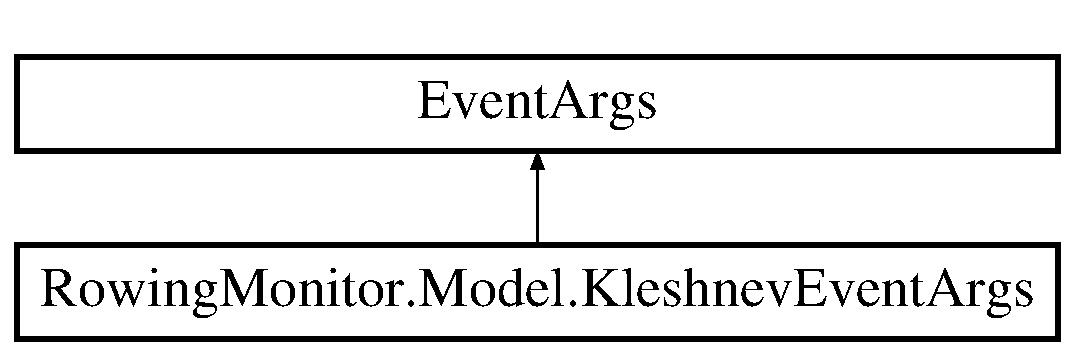
\includegraphics[height=2.000000cm]{class_rowing_monitor_1_1_model_1_1_kleshnev_event_args}
\end{center}
\end{figure}
\subsection*{Public Member Functions}
\begin{DoxyCompactItemize}
\item 
\hyperlink{class_rowing_monitor_1_1_model_1_1_kleshnev_event_args_ad371c1b70b890d6991665a29120fb554}{Kleshnev\+Event\+Args} (List$<$ \hyperlink{struct_rowing_monitor_1_1_model_1_1_pipeline_1_1_kleshnev_data}{Kleshnev\+Data} $>$ kleshnev\+Data)
\end{DoxyCompactItemize}


\subsection{Detailed Description}
Represents the arguments for a finished Kleshnev analysis. 



\subsection{Constructor \& Destructor Documentation}
\mbox{\Hypertarget{class_rowing_monitor_1_1_model_1_1_kleshnev_event_args_ad371c1b70b890d6991665a29120fb554}\label{class_rowing_monitor_1_1_model_1_1_kleshnev_event_args_ad371c1b70b890d6991665a29120fb554}} 
\index{Rowing\+Monitor\+::\+Model\+::\+Kleshnev\+Event\+Args@{Rowing\+Monitor\+::\+Model\+::\+Kleshnev\+Event\+Args}!Kleshnev\+Event\+Args@{Kleshnev\+Event\+Args}}
\index{Kleshnev\+Event\+Args@{Kleshnev\+Event\+Args}!Rowing\+Monitor\+::\+Model\+::\+Kleshnev\+Event\+Args@{Rowing\+Monitor\+::\+Model\+::\+Kleshnev\+Event\+Args}}
\subsubsection{\texorpdfstring{Kleshnev\+Event\+Args()}{KleshnevEventArgs()}}
{\footnotesize\ttfamily Rowing\+Monitor.\+Model.\+Kleshnev\+Event\+Args.\+Kleshnev\+Event\+Args (\begin{DoxyParamCaption}\item[{List$<$ \hyperlink{struct_rowing_monitor_1_1_model_1_1_pipeline_1_1_kleshnev_data}{Kleshnev\+Data} $>$}]{kleshnev\+Data }\end{DoxyParamCaption})}



The documentation for this class was generated from the following file\+:\begin{DoxyCompactItemize}
\item 
Model/\+Event\+Args/\hyperlink{_kleshnev_event_args_8cs}{Kleshnev\+Event\+Args.\+cs}\end{DoxyCompactItemize}

\hypertarget{class_rowing_monitor_1_1_model_1_1_pipeline_1_1_kleshnev_velocity_calculator}{}\section{Rowing\+Monitor.\+Model.\+Pipeline.\+Kleshnev\+Velocity\+Calculator Class Reference}
\label{class_rowing_monitor_1_1_model_1_1_pipeline_1_1_kleshnev_velocity_calculator}\index{Rowing\+Monitor.\+Model.\+Pipeline.\+Kleshnev\+Velocity\+Calculator@{Rowing\+Monitor.\+Model.\+Pipeline.\+Kleshnev\+Velocity\+Calculator}}
\subsection*{Public Member Functions}
\begin{DoxyCompactItemize}
\item 
delegate void \hyperlink{class_rowing_monitor_1_1_model_1_1_pipeline_1_1_kleshnev_velocity_calculator_aa8c251dc416d32f364bf138f4abeada7}{Kleshnev\+Calculation\+Finished\+Event\+Handler} (Object sender, \hyperlink{class_rowing_monitor_1_1_model_1_1_kleshnev_event_args}{Kleshnev\+Event\+Args} e)
\item 
\hyperlink{class_rowing_monitor_1_1_model_1_1_pipeline_1_1_kleshnev_velocity_calculator_ae642d137281c0ce38a84300066b28a64}{Kleshnev\+Velocity\+Calculator} ()
\item 
void \hyperlink{class_rowing_monitor_1_1_model_1_1_pipeline_1_1_kleshnev_velocity_calculator_af2ff2cb627827d1167732566636cc593}{Update} (\hyperlink{struct_rowing_monitor_1_1_model_1_1_util_1_1_joint_data}{Joint\+Data} joint\+Data)
\item 
List$<$ \hyperlink{struct_rowing_monitor_1_1_model_1_1_pipeline_1_1_kleshnev_data}{Kleshnev\+Data} $>$ \hyperlink{class_rowing_monitor_1_1_model_1_1_pipeline_1_1_kleshnev_velocity_calculator_a24776dfe3d1a8d3a499bfa48e721a868}{Calculate\+Kleshnev\+Velocities} (\hyperlink{struct_rowing_monitor_1_1_model_1_1_util_1_1_joint_data}{Joint\+Data} velocity\+Joint\+Data)
\end{DoxyCompactItemize}
\subsection*{Properties}
\begin{DoxyCompactItemize}
\item 
Broadcast\+Block$<$ \hyperlink{struct_rowing_monitor_1_1_model_1_1_pipeline_1_1_kleshnev_data}{Kleshnev\+Data} $>$ \hyperlink{class_rowing_monitor_1_1_model_1_1_pipeline_1_1_kleshnev_velocity_calculator_aed5495aa6d896a442ce39926ee30ed2c}{Output}\hspace{0.3cm}{\ttfamily  \mbox{[}get, set\mbox{]}}
\item 
Action\+Block$<$ \hyperlink{struct_rowing_monitor_1_1_model_1_1_util_1_1_joint_data}{Joint\+Data} $>$ \hyperlink{class_rowing_monitor_1_1_model_1_1_pipeline_1_1_kleshnev_velocity_calculator_a87c25ad950ba36047df4367a3a90cd20}{Input}\hspace{0.3cm}{\ttfamily  \mbox{[}get, set\mbox{]}}
\end{DoxyCompactItemize}
\subsection*{Events}
\begin{DoxyCompactItemize}
\item 
\hyperlink{class_rowing_monitor_1_1_model_1_1_pipeline_1_1_kleshnev_velocity_calculator_aa8c251dc416d32f364bf138f4abeada7}{Kleshnev\+Calculation\+Finished\+Event\+Handler} \hyperlink{class_rowing_monitor_1_1_model_1_1_pipeline_1_1_kleshnev_velocity_calculator_afc60a4e7b76e1bfd9c12b5aacda05a51}{Kleshnev\+Calculation\+Finished}
\end{DoxyCompactItemize}


\subsection{Constructor \& Destructor Documentation}
\mbox{\Hypertarget{class_rowing_monitor_1_1_model_1_1_pipeline_1_1_kleshnev_velocity_calculator_ae642d137281c0ce38a84300066b28a64}\label{class_rowing_monitor_1_1_model_1_1_pipeline_1_1_kleshnev_velocity_calculator_ae642d137281c0ce38a84300066b28a64}} 
\index{Rowing\+Monitor\+::\+Model\+::\+Pipeline\+::\+Kleshnev\+Velocity\+Calculator@{Rowing\+Monitor\+::\+Model\+::\+Pipeline\+::\+Kleshnev\+Velocity\+Calculator}!Kleshnev\+Velocity\+Calculator@{Kleshnev\+Velocity\+Calculator}}
\index{Kleshnev\+Velocity\+Calculator@{Kleshnev\+Velocity\+Calculator}!Rowing\+Monitor\+::\+Model\+::\+Pipeline\+::\+Kleshnev\+Velocity\+Calculator@{Rowing\+Monitor\+::\+Model\+::\+Pipeline\+::\+Kleshnev\+Velocity\+Calculator}}
\subsubsection{\texorpdfstring{Kleshnev\+Velocity\+Calculator()}{KleshnevVelocityCalculator()}}
{\footnotesize\ttfamily Rowing\+Monitor.\+Model.\+Pipeline.\+Kleshnev\+Velocity\+Calculator.\+Kleshnev\+Velocity\+Calculator (\begin{DoxyParamCaption}{ }\end{DoxyParamCaption})}



\subsection{Member Function Documentation}
\mbox{\Hypertarget{class_rowing_monitor_1_1_model_1_1_pipeline_1_1_kleshnev_velocity_calculator_a24776dfe3d1a8d3a499bfa48e721a868}\label{class_rowing_monitor_1_1_model_1_1_pipeline_1_1_kleshnev_velocity_calculator_a24776dfe3d1a8d3a499bfa48e721a868}} 
\index{Rowing\+Monitor\+::\+Model\+::\+Pipeline\+::\+Kleshnev\+Velocity\+Calculator@{Rowing\+Monitor\+::\+Model\+::\+Pipeline\+::\+Kleshnev\+Velocity\+Calculator}!Calculate\+Kleshnev\+Velocities@{Calculate\+Kleshnev\+Velocities}}
\index{Calculate\+Kleshnev\+Velocities@{Calculate\+Kleshnev\+Velocities}!Rowing\+Monitor\+::\+Model\+::\+Pipeline\+::\+Kleshnev\+Velocity\+Calculator@{Rowing\+Monitor\+::\+Model\+::\+Pipeline\+::\+Kleshnev\+Velocity\+Calculator}}
\subsubsection{\texorpdfstring{Calculate\+Kleshnev\+Velocities()}{CalculateKleshnevVelocities()}}
{\footnotesize\ttfamily List$<$\hyperlink{struct_rowing_monitor_1_1_model_1_1_pipeline_1_1_kleshnev_data}{Kleshnev\+Data}$>$ Rowing\+Monitor.\+Model.\+Pipeline.\+Kleshnev\+Velocity\+Calculator.\+Calculate\+Kleshnev\+Velocities (\begin{DoxyParamCaption}\item[{\hyperlink{struct_rowing_monitor_1_1_model_1_1_util_1_1_joint_data}{Joint\+Data}}]{velocity\+Joint\+Data }\end{DoxyParamCaption})}

\mbox{\Hypertarget{class_rowing_monitor_1_1_model_1_1_pipeline_1_1_kleshnev_velocity_calculator_aa8c251dc416d32f364bf138f4abeada7}\label{class_rowing_monitor_1_1_model_1_1_pipeline_1_1_kleshnev_velocity_calculator_aa8c251dc416d32f364bf138f4abeada7}} 
\index{Rowing\+Monitor\+::\+Model\+::\+Pipeline\+::\+Kleshnev\+Velocity\+Calculator@{Rowing\+Monitor\+::\+Model\+::\+Pipeline\+::\+Kleshnev\+Velocity\+Calculator}!Kleshnev\+Calculation\+Finished\+Event\+Handler@{Kleshnev\+Calculation\+Finished\+Event\+Handler}}
\index{Kleshnev\+Calculation\+Finished\+Event\+Handler@{Kleshnev\+Calculation\+Finished\+Event\+Handler}!Rowing\+Monitor\+::\+Model\+::\+Pipeline\+::\+Kleshnev\+Velocity\+Calculator@{Rowing\+Monitor\+::\+Model\+::\+Pipeline\+::\+Kleshnev\+Velocity\+Calculator}}
\subsubsection{\texorpdfstring{Kleshnev\+Calculation\+Finished\+Event\+Handler()}{KleshnevCalculationFinishedEventHandler()}}
{\footnotesize\ttfamily delegate void Rowing\+Monitor.\+Model.\+Pipeline.\+Kleshnev\+Velocity\+Calculator.\+Kleshnev\+Calculation\+Finished\+Event\+Handler (\begin{DoxyParamCaption}\item[{Object}]{sender,  }\item[{\hyperlink{class_rowing_monitor_1_1_model_1_1_kleshnev_event_args}{Kleshnev\+Event\+Args}}]{e }\end{DoxyParamCaption})}

\mbox{\Hypertarget{class_rowing_monitor_1_1_model_1_1_pipeline_1_1_kleshnev_velocity_calculator_af2ff2cb627827d1167732566636cc593}\label{class_rowing_monitor_1_1_model_1_1_pipeline_1_1_kleshnev_velocity_calculator_af2ff2cb627827d1167732566636cc593}} 
\index{Rowing\+Monitor\+::\+Model\+::\+Pipeline\+::\+Kleshnev\+Velocity\+Calculator@{Rowing\+Monitor\+::\+Model\+::\+Pipeline\+::\+Kleshnev\+Velocity\+Calculator}!Update@{Update}}
\index{Update@{Update}!Rowing\+Monitor\+::\+Model\+::\+Pipeline\+::\+Kleshnev\+Velocity\+Calculator@{Rowing\+Monitor\+::\+Model\+::\+Pipeline\+::\+Kleshnev\+Velocity\+Calculator}}
\subsubsection{\texorpdfstring{Update()}{Update()}}
{\footnotesize\ttfamily void Rowing\+Monitor.\+Model.\+Pipeline.\+Kleshnev\+Velocity\+Calculator.\+Update (\begin{DoxyParamCaption}\item[{\hyperlink{struct_rowing_monitor_1_1_model_1_1_util_1_1_joint_data}{Joint\+Data}}]{joint\+Data }\end{DoxyParamCaption})}



\subsection{Property Documentation}
\mbox{\Hypertarget{class_rowing_monitor_1_1_model_1_1_pipeline_1_1_kleshnev_velocity_calculator_a87c25ad950ba36047df4367a3a90cd20}\label{class_rowing_monitor_1_1_model_1_1_pipeline_1_1_kleshnev_velocity_calculator_a87c25ad950ba36047df4367a3a90cd20}} 
\index{Rowing\+Monitor\+::\+Model\+::\+Pipeline\+::\+Kleshnev\+Velocity\+Calculator@{Rowing\+Monitor\+::\+Model\+::\+Pipeline\+::\+Kleshnev\+Velocity\+Calculator}!Input@{Input}}
\index{Input@{Input}!Rowing\+Monitor\+::\+Model\+::\+Pipeline\+::\+Kleshnev\+Velocity\+Calculator@{Rowing\+Monitor\+::\+Model\+::\+Pipeline\+::\+Kleshnev\+Velocity\+Calculator}}
\subsubsection{\texorpdfstring{Input}{Input}}
{\footnotesize\ttfamily Action\+Block$<$\hyperlink{struct_rowing_monitor_1_1_model_1_1_util_1_1_joint_data}{Joint\+Data}$>$ Rowing\+Monitor.\+Model.\+Pipeline.\+Kleshnev\+Velocity\+Calculator.\+Input\hspace{0.3cm}{\ttfamily [get]}, {\ttfamily [set]}}

\mbox{\Hypertarget{class_rowing_monitor_1_1_model_1_1_pipeline_1_1_kleshnev_velocity_calculator_aed5495aa6d896a442ce39926ee30ed2c}\label{class_rowing_monitor_1_1_model_1_1_pipeline_1_1_kleshnev_velocity_calculator_aed5495aa6d896a442ce39926ee30ed2c}} 
\index{Rowing\+Monitor\+::\+Model\+::\+Pipeline\+::\+Kleshnev\+Velocity\+Calculator@{Rowing\+Monitor\+::\+Model\+::\+Pipeline\+::\+Kleshnev\+Velocity\+Calculator}!Output@{Output}}
\index{Output@{Output}!Rowing\+Monitor\+::\+Model\+::\+Pipeline\+::\+Kleshnev\+Velocity\+Calculator@{Rowing\+Monitor\+::\+Model\+::\+Pipeline\+::\+Kleshnev\+Velocity\+Calculator}}
\subsubsection{\texorpdfstring{Output}{Output}}
{\footnotesize\ttfamily Broadcast\+Block$<$\hyperlink{struct_rowing_monitor_1_1_model_1_1_pipeline_1_1_kleshnev_data}{Kleshnev\+Data}$>$ Rowing\+Monitor.\+Model.\+Pipeline.\+Kleshnev\+Velocity\+Calculator.\+Output\hspace{0.3cm}{\ttfamily [get]}, {\ttfamily [set]}}



\subsection{Event Documentation}
\mbox{\Hypertarget{class_rowing_monitor_1_1_model_1_1_pipeline_1_1_kleshnev_velocity_calculator_afc60a4e7b76e1bfd9c12b5aacda05a51}\label{class_rowing_monitor_1_1_model_1_1_pipeline_1_1_kleshnev_velocity_calculator_afc60a4e7b76e1bfd9c12b5aacda05a51}} 
\index{Rowing\+Monitor\+::\+Model\+::\+Pipeline\+::\+Kleshnev\+Velocity\+Calculator@{Rowing\+Monitor\+::\+Model\+::\+Pipeline\+::\+Kleshnev\+Velocity\+Calculator}!Kleshnev\+Calculation\+Finished@{Kleshnev\+Calculation\+Finished}}
\index{Kleshnev\+Calculation\+Finished@{Kleshnev\+Calculation\+Finished}!Rowing\+Monitor\+::\+Model\+::\+Pipeline\+::\+Kleshnev\+Velocity\+Calculator@{Rowing\+Monitor\+::\+Model\+::\+Pipeline\+::\+Kleshnev\+Velocity\+Calculator}}
\subsubsection{\texorpdfstring{Kleshnev\+Calculation\+Finished}{KleshnevCalculationFinished}}
{\footnotesize\ttfamily \hyperlink{class_rowing_monitor_1_1_model_1_1_pipeline_1_1_kleshnev_velocity_calculator_aa8c251dc416d32f364bf138f4abeada7}{Kleshnev\+Calculation\+Finished\+Event\+Handler} Rowing\+Monitor.\+Model.\+Pipeline.\+Kleshnev\+Velocity\+Calculator.\+Kleshnev\+Calculation\+Finished}



The documentation for this class was generated from the following file\+:\begin{DoxyCompactItemize}
\item 
Model/\+Pipeline/\hyperlink{_kleshnev_velocity_calculator_8cs}{Kleshnev\+Velocity\+Calculator.\+cs}\end{DoxyCompactItemize}

\hypertarget{class_rowing_monitor_1_1_model_1_1_low_pass_filter}{}\section{Rowing\+Monitor.\+Model.\+Low\+Pass\+Filter Class Reference}
\label{class_rowing_monitor_1_1_model_1_1_low_pass_filter}\index{Rowing\+Monitor.\+Model.\+Low\+Pass\+Filter@{Rowing\+Monitor.\+Model.\+Low\+Pass\+Filter}}
\subsection*{Public Member Functions}
\begin{DoxyCompactItemize}
\item 
\hyperlink{class_rowing_monitor_1_1_model_1_1_low_pass_filter_ae2409a1bea75885b3de02c300f46bb68}{Low\+Pass\+Filter} ()
\item 
Dictionary$<$ Joint\+Type, Joint $>$ \hyperlink{class_rowing_monitor_1_1_model_1_1_low_pass_filter_abd95054e31280d78ad6d0d4a5bd106ea}{Filter} (Dictionary$<$ Joint\+Type, Joint $>$ joints, Dictionary$<$ Joint\+Type, Dictionary$<$ String, Double $>$$>$ alpha)
\end{DoxyCompactItemize}
\subsection*{Properties}
\begin{DoxyCompactItemize}
\item 
Dictionary$<$ Joint\+Type, Joint $>$ \hyperlink{class_rowing_monitor_1_1_model_1_1_low_pass_filter_ab5c930d79699ed13c290b56a9d4501c6}{Hatxprev}\hspace{0.3cm}{\ttfamily  \mbox{[}get\mbox{]}}
\end{DoxyCompactItemize}


\subsection{Constructor \& Destructor Documentation}
\mbox{\Hypertarget{class_rowing_monitor_1_1_model_1_1_low_pass_filter_ae2409a1bea75885b3de02c300f46bb68}\label{class_rowing_monitor_1_1_model_1_1_low_pass_filter_ae2409a1bea75885b3de02c300f46bb68}} 
\index{Rowing\+Monitor\+::\+Model\+::\+Low\+Pass\+Filter@{Rowing\+Monitor\+::\+Model\+::\+Low\+Pass\+Filter}!Low\+Pass\+Filter@{Low\+Pass\+Filter}}
\index{Low\+Pass\+Filter@{Low\+Pass\+Filter}!Rowing\+Monitor\+::\+Model\+::\+Low\+Pass\+Filter@{Rowing\+Monitor\+::\+Model\+::\+Low\+Pass\+Filter}}
\subsubsection{\texorpdfstring{Low\+Pass\+Filter()}{LowPassFilter()}}
{\footnotesize\ttfamily Rowing\+Monitor.\+Model.\+Low\+Pass\+Filter.\+Low\+Pass\+Filter (\begin{DoxyParamCaption}{ }\end{DoxyParamCaption})}



\subsection{Member Function Documentation}
\mbox{\Hypertarget{class_rowing_monitor_1_1_model_1_1_low_pass_filter_abd95054e31280d78ad6d0d4a5bd106ea}\label{class_rowing_monitor_1_1_model_1_1_low_pass_filter_abd95054e31280d78ad6d0d4a5bd106ea}} 
\index{Rowing\+Monitor\+::\+Model\+::\+Low\+Pass\+Filter@{Rowing\+Monitor\+::\+Model\+::\+Low\+Pass\+Filter}!Filter@{Filter}}
\index{Filter@{Filter}!Rowing\+Monitor\+::\+Model\+::\+Low\+Pass\+Filter@{Rowing\+Monitor\+::\+Model\+::\+Low\+Pass\+Filter}}
\subsubsection{\texorpdfstring{Filter()}{Filter()}}
{\footnotesize\ttfamily Dictionary$<$Joint\+Type, Joint$>$ Rowing\+Monitor.\+Model.\+Low\+Pass\+Filter.\+Filter (\begin{DoxyParamCaption}\item[{Dictionary$<$ Joint\+Type, Joint $>$}]{joints,  }\item[{Dictionary$<$ Joint\+Type, Dictionary$<$ String, Double $>$$>$}]{alpha }\end{DoxyParamCaption})}



\subsection{Property Documentation}
\mbox{\Hypertarget{class_rowing_monitor_1_1_model_1_1_low_pass_filter_ab5c930d79699ed13c290b56a9d4501c6}\label{class_rowing_monitor_1_1_model_1_1_low_pass_filter_ab5c930d79699ed13c290b56a9d4501c6}} 
\index{Rowing\+Monitor\+::\+Model\+::\+Low\+Pass\+Filter@{Rowing\+Monitor\+::\+Model\+::\+Low\+Pass\+Filter}!Hatxprev@{Hatxprev}}
\index{Hatxprev@{Hatxprev}!Rowing\+Monitor\+::\+Model\+::\+Low\+Pass\+Filter@{Rowing\+Monitor\+::\+Model\+::\+Low\+Pass\+Filter}}
\subsubsection{\texorpdfstring{Hatxprev}{Hatxprev}}
{\footnotesize\ttfamily Dictionary$<$Joint\+Type, Joint$>$ Rowing\+Monitor.\+Model.\+Low\+Pass\+Filter.\+Hatxprev\hspace{0.3cm}{\ttfamily [get]}}



The documentation for this class was generated from the following file\+:\begin{DoxyCompactItemize}
\item 
Model/\+Util/\hyperlink{_low_pass_filter_8cs}{Low\+Pass\+Filter.\+cs}\end{DoxyCompactItemize}

\hypertarget{class_rowing_monitor_1_1_view_model_1_1_main_view_model}{}\section{Rowing\+Monitor.\+View\+Model.\+Main\+View\+Model Class Reference}
\label{class_rowing_monitor_1_1_view_model_1_1_main_view_model}\index{Rowing\+Monitor.\+View\+Model.\+Main\+View\+Model@{Rowing\+Monitor.\+View\+Model.\+Main\+View\+Model}}


Represents the view-\/model for the main window.  


Inheritance diagram for Rowing\+Monitor.\+View\+Model.\+Main\+View\+Model\+:\begin{figure}[H]
\begin{center}
\leavevmode
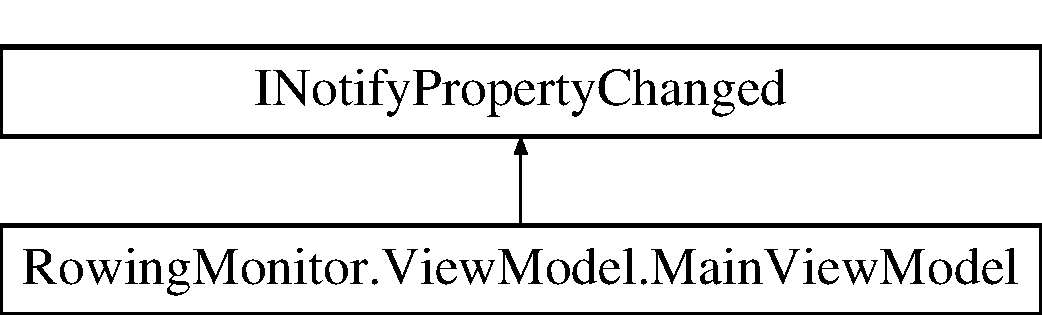
\includegraphics[height=2.000000cm]{class_rowing_monitor_1_1_view_model_1_1_main_view_model}
\end{center}
\end{figure}
\subsection*{Public Member Functions}
\begin{DoxyCompactItemize}
\item 
\hyperlink{class_rowing_monitor_1_1_view_model_1_1_main_view_model_a52869d6dbed480afdc4bdebf10d4ff15}{Main\+View\+Model} ()
\begin{DoxyCompactList}\small\item\em Initializes a new instance of the \hyperlink{class_rowing_monitor_1_1_view_model_1_1_main_view_model}{Main\+View\+Model} class. \end{DoxyCompactList}\end{DoxyCompactItemize}
\subsection*{Protected Member Functions}
\begin{DoxyCompactItemize}
\item 
void \hyperlink{class_rowing_monitor_1_1_view_model_1_1_main_view_model_afd603b400bc0a127b8005f09850fede0}{Raise\+Property\+Changed} (string property)
\end{DoxyCompactItemize}
\subsection*{Properties}
\begin{DoxyCompactItemize}
\item 
I\+Command \hyperlink{class_rowing_monitor_1_1_view_model_1_1_main_view_model_a41b14c5d964f16872ba4ff7e902d086a}{Window\+Loaded}\hspace{0.3cm}{\ttfamily  \mbox{[}get\mbox{]}}
\item 
I\+Command \hyperlink{class_rowing_monitor_1_1_view_model_1_1_main_view_model_abf7344a3fb92d215e85568c2b8ea2413}{Window\+Closing}\hspace{0.3cm}{\ttfamily  \mbox{[}get\mbox{]}}
\item 
Image\+Source \hyperlink{class_rowing_monitor_1_1_view_model_1_1_main_view_model_a8db6c0be0de3d081ecc1cfd4e29f63ea}{Body\+Image\+Source}\hspace{0.3cm}{\ttfamily  \mbox{[}get, set\mbox{]}}
\item 
Image\+Source \hyperlink{class_rowing_monitor_1_1_view_model_1_1_main_view_model_a855a4d13248cb58ac588e6993674f371}{Side\+Body\+Image\+Source}\hspace{0.3cm}{\ttfamily  \mbox{[}get, set\mbox{]}}
\item 
Image\+Source \hyperlink{class_rowing_monitor_1_1_view_model_1_1_main_view_model_a6a3397050ea6774eabf6118819a183a0}{Color\+Image\+Source}\hspace{0.3cm}{\ttfamily  \mbox{[}get, set\mbox{]}}
\item 
double \hyperlink{class_rowing_monitor_1_1_view_model_1_1_main_view_model_aea1ee41eb29904df4dd08c781def6bd2}{Beta}\hspace{0.3cm}{\ttfamily  \mbox{[}get, set\mbox{]}}
\item 
double \hyperlink{class_rowing_monitor_1_1_view_model_1_1_main_view_model_a4008baa81a327f935e14c4024b5b0d9d}{Fcmin}\hspace{0.3cm}{\ttfamily  \mbox{[}get, set\mbox{]}}
\item 
List$<$ Joint\+Type $>$ \hyperlink{class_rowing_monitor_1_1_view_model_1_1_main_view_model_a0b81c01247d969c5e5f3ba913f48c31d}{Plot\+Joint\+Types}\hspace{0.3cm}{\ttfamily  \mbox{[}get, set\mbox{]}}
\item 
List$<$ \hyperlink{namespace_rowing_monitor_1_1_model_1_1_util_a01e1a06061533b246feb7421c9d0107f}{Model.\+Util.\+Data\+Stream\+Type} $>$ \hyperlink{class_rowing_monitor_1_1_view_model_1_1_main_view_model_a6887b1eb891b47726c699746a480e9fb}{Plot\+Measured\+Variables}\hspace{0.3cm}{\ttfamily  \mbox{[}get, set\mbox{]}}
\item 
bool \hyperlink{class_rowing_monitor_1_1_view_model_1_1_main_view_model_a8cbb8130173da1515292ed6b0841ddb2}{Use\+Kinect\+Joint\+Filter}\hspace{0.3cm}{\ttfamily  \mbox{[}get, set\mbox{]}}
\item 
bool \hyperlink{class_rowing_monitor_1_1_view_model_1_1_main_view_model_afedc4cf51fc351066048b9b30b69aa45}{Use\+Z\+VC}\hspace{0.3cm}{\ttfamily  \mbox{[}get, set\mbox{]}}
\item 
Plot\+Model \hyperlink{class_rowing_monitor_1_1_view_model_1_1_main_view_model_a79c8374c2e47f0d83d1a7561a078c6c7}{Default\+Plot\+Model}\hspace{0.3cm}{\ttfamily  \mbox{[}get\mbox{]}}
\item 
Plot\+Model \hyperlink{class_rowing_monitor_1_1_view_model_1_1_main_view_model_a96719ac6ef51316ea6149ee4b2a0b299}{Klsh\+Last\+Segment\+Plot\+Model}\hspace{0.3cm}{\ttfamily  \mbox{[}get\mbox{]}}
\item 
Plot\+Model \hyperlink{class_rowing_monitor_1_1_view_model_1_1_main_view_model_a9534f6ef9053f21582f5e16da72441c0}{Klsh\+Current\+Segment\+Plot\+Model}\hspace{0.3cm}{\ttfamily  \mbox{[}get\mbox{]}}
\end{DoxyCompactItemize}
\subsection*{Events}
\begin{DoxyCompactItemize}
\item 
Property\+Changed\+Event\+Handler \hyperlink{class_rowing_monitor_1_1_view_model_1_1_main_view_model_ab8b22b1f06c2bb51fb1a162055adeb47}{Property\+Changed}
\begin{DoxyCompactList}\small\item\em I\+Notify\+Property\+Changed\+Property\+Changed event to allow window controls to bind to changeable data \end{DoxyCompactList}\end{DoxyCompactItemize}


\subsection{Detailed Description}
Represents the view-\/model for the main window. 



\subsection{Constructor \& Destructor Documentation}
\mbox{\Hypertarget{class_rowing_monitor_1_1_view_model_1_1_main_view_model_a52869d6dbed480afdc4bdebf10d4ff15}\label{class_rowing_monitor_1_1_view_model_1_1_main_view_model_a52869d6dbed480afdc4bdebf10d4ff15}} 
\index{Rowing\+Monitor\+::\+View\+Model\+::\+Main\+View\+Model@{Rowing\+Monitor\+::\+View\+Model\+::\+Main\+View\+Model}!Main\+View\+Model@{Main\+View\+Model}}
\index{Main\+View\+Model@{Main\+View\+Model}!Rowing\+Monitor\+::\+View\+Model\+::\+Main\+View\+Model@{Rowing\+Monitor\+::\+View\+Model\+::\+Main\+View\+Model}}
\subsubsection{\texorpdfstring{Main\+View\+Model()}{MainViewModel()}}
{\footnotesize\ttfamily Rowing\+Monitor.\+View\+Model.\+Main\+View\+Model.\+Main\+View\+Model (\begin{DoxyParamCaption}{ }\end{DoxyParamCaption})}



Initializes a new instance of the \hyperlink{class_rowing_monitor_1_1_view_model_1_1_main_view_model}{Main\+View\+Model} class. 



\subsection{Member Function Documentation}
\mbox{\Hypertarget{class_rowing_monitor_1_1_view_model_1_1_main_view_model_afd603b400bc0a127b8005f09850fede0}\label{class_rowing_monitor_1_1_view_model_1_1_main_view_model_afd603b400bc0a127b8005f09850fede0}} 
\index{Rowing\+Monitor\+::\+View\+Model\+::\+Main\+View\+Model@{Rowing\+Monitor\+::\+View\+Model\+::\+Main\+View\+Model}!Raise\+Property\+Changed@{Raise\+Property\+Changed}}
\index{Raise\+Property\+Changed@{Raise\+Property\+Changed}!Rowing\+Monitor\+::\+View\+Model\+::\+Main\+View\+Model@{Rowing\+Monitor\+::\+View\+Model\+::\+Main\+View\+Model}}
\subsubsection{\texorpdfstring{Raise\+Property\+Changed()}{RaisePropertyChanged()}}
{\footnotesize\ttfamily void Rowing\+Monitor.\+View\+Model.\+Main\+View\+Model.\+Raise\+Property\+Changed (\begin{DoxyParamCaption}\item[{string}]{property }\end{DoxyParamCaption})\hspace{0.3cm}{\ttfamily [protected]}}



\subsection{Property Documentation}
\mbox{\Hypertarget{class_rowing_monitor_1_1_view_model_1_1_main_view_model_aea1ee41eb29904df4dd08c781def6bd2}\label{class_rowing_monitor_1_1_view_model_1_1_main_view_model_aea1ee41eb29904df4dd08c781def6bd2}} 
\index{Rowing\+Monitor\+::\+View\+Model\+::\+Main\+View\+Model@{Rowing\+Monitor\+::\+View\+Model\+::\+Main\+View\+Model}!Beta@{Beta}}
\index{Beta@{Beta}!Rowing\+Monitor\+::\+View\+Model\+::\+Main\+View\+Model@{Rowing\+Monitor\+::\+View\+Model\+::\+Main\+View\+Model}}
\subsubsection{\texorpdfstring{Beta}{Beta}}
{\footnotesize\ttfamily double Rowing\+Monitor.\+View\+Model.\+Main\+View\+Model.\+Beta\hspace{0.3cm}{\ttfamily [get]}, {\ttfamily [set]}}

\mbox{\Hypertarget{class_rowing_monitor_1_1_view_model_1_1_main_view_model_a8db6c0be0de3d081ecc1cfd4e29f63ea}\label{class_rowing_monitor_1_1_view_model_1_1_main_view_model_a8db6c0be0de3d081ecc1cfd4e29f63ea}} 
\index{Rowing\+Monitor\+::\+View\+Model\+::\+Main\+View\+Model@{Rowing\+Monitor\+::\+View\+Model\+::\+Main\+View\+Model}!Body\+Image\+Source@{Body\+Image\+Source}}
\index{Body\+Image\+Source@{Body\+Image\+Source}!Rowing\+Monitor\+::\+View\+Model\+::\+Main\+View\+Model@{Rowing\+Monitor\+::\+View\+Model\+::\+Main\+View\+Model}}
\subsubsection{\texorpdfstring{Body\+Image\+Source}{BodyImageSource}}
{\footnotesize\ttfamily Image\+Source Rowing\+Monitor.\+View\+Model.\+Main\+View\+Model.\+Body\+Image\+Source\hspace{0.3cm}{\ttfamily [get]}, {\ttfamily [set]}}

\mbox{\Hypertarget{class_rowing_monitor_1_1_view_model_1_1_main_view_model_a6a3397050ea6774eabf6118819a183a0}\label{class_rowing_monitor_1_1_view_model_1_1_main_view_model_a6a3397050ea6774eabf6118819a183a0}} 
\index{Rowing\+Monitor\+::\+View\+Model\+::\+Main\+View\+Model@{Rowing\+Monitor\+::\+View\+Model\+::\+Main\+View\+Model}!Color\+Image\+Source@{Color\+Image\+Source}}
\index{Color\+Image\+Source@{Color\+Image\+Source}!Rowing\+Monitor\+::\+View\+Model\+::\+Main\+View\+Model@{Rowing\+Monitor\+::\+View\+Model\+::\+Main\+View\+Model}}
\subsubsection{\texorpdfstring{Color\+Image\+Source}{ColorImageSource}}
{\footnotesize\ttfamily Image\+Source Rowing\+Monitor.\+View\+Model.\+Main\+View\+Model.\+Color\+Image\+Source\hspace{0.3cm}{\ttfamily [get]}, {\ttfamily [set]}}

\mbox{\Hypertarget{class_rowing_monitor_1_1_view_model_1_1_main_view_model_a79c8374c2e47f0d83d1a7561a078c6c7}\label{class_rowing_monitor_1_1_view_model_1_1_main_view_model_a79c8374c2e47f0d83d1a7561a078c6c7}} 
\index{Rowing\+Monitor\+::\+View\+Model\+::\+Main\+View\+Model@{Rowing\+Monitor\+::\+View\+Model\+::\+Main\+View\+Model}!Default\+Plot\+Model@{Default\+Plot\+Model}}
\index{Default\+Plot\+Model@{Default\+Plot\+Model}!Rowing\+Monitor\+::\+View\+Model\+::\+Main\+View\+Model@{Rowing\+Monitor\+::\+View\+Model\+::\+Main\+View\+Model}}
\subsubsection{\texorpdfstring{Default\+Plot\+Model}{DefaultPlotModel}}
{\footnotesize\ttfamily Plot\+Model Rowing\+Monitor.\+View\+Model.\+Main\+View\+Model.\+Default\+Plot\+Model\hspace{0.3cm}{\ttfamily [get]}}

\mbox{\Hypertarget{class_rowing_monitor_1_1_view_model_1_1_main_view_model_a4008baa81a327f935e14c4024b5b0d9d}\label{class_rowing_monitor_1_1_view_model_1_1_main_view_model_a4008baa81a327f935e14c4024b5b0d9d}} 
\index{Rowing\+Monitor\+::\+View\+Model\+::\+Main\+View\+Model@{Rowing\+Monitor\+::\+View\+Model\+::\+Main\+View\+Model}!Fcmin@{Fcmin}}
\index{Fcmin@{Fcmin}!Rowing\+Monitor\+::\+View\+Model\+::\+Main\+View\+Model@{Rowing\+Monitor\+::\+View\+Model\+::\+Main\+View\+Model}}
\subsubsection{\texorpdfstring{Fcmin}{Fcmin}}
{\footnotesize\ttfamily double Rowing\+Monitor.\+View\+Model.\+Main\+View\+Model.\+Fcmin\hspace{0.3cm}{\ttfamily [get]}, {\ttfamily [set]}}

\mbox{\Hypertarget{class_rowing_monitor_1_1_view_model_1_1_main_view_model_a9534f6ef9053f21582f5e16da72441c0}\label{class_rowing_monitor_1_1_view_model_1_1_main_view_model_a9534f6ef9053f21582f5e16da72441c0}} 
\index{Rowing\+Monitor\+::\+View\+Model\+::\+Main\+View\+Model@{Rowing\+Monitor\+::\+View\+Model\+::\+Main\+View\+Model}!Klsh\+Current\+Segment\+Plot\+Model@{Klsh\+Current\+Segment\+Plot\+Model}}
\index{Klsh\+Current\+Segment\+Plot\+Model@{Klsh\+Current\+Segment\+Plot\+Model}!Rowing\+Monitor\+::\+View\+Model\+::\+Main\+View\+Model@{Rowing\+Monitor\+::\+View\+Model\+::\+Main\+View\+Model}}
\subsubsection{\texorpdfstring{Klsh\+Current\+Segment\+Plot\+Model}{KlshCurrentSegmentPlotModel}}
{\footnotesize\ttfamily Plot\+Model Rowing\+Monitor.\+View\+Model.\+Main\+View\+Model.\+Klsh\+Current\+Segment\+Plot\+Model\hspace{0.3cm}{\ttfamily [get]}}

\mbox{\Hypertarget{class_rowing_monitor_1_1_view_model_1_1_main_view_model_a96719ac6ef51316ea6149ee4b2a0b299}\label{class_rowing_monitor_1_1_view_model_1_1_main_view_model_a96719ac6ef51316ea6149ee4b2a0b299}} 
\index{Rowing\+Monitor\+::\+View\+Model\+::\+Main\+View\+Model@{Rowing\+Monitor\+::\+View\+Model\+::\+Main\+View\+Model}!Klsh\+Last\+Segment\+Plot\+Model@{Klsh\+Last\+Segment\+Plot\+Model}}
\index{Klsh\+Last\+Segment\+Plot\+Model@{Klsh\+Last\+Segment\+Plot\+Model}!Rowing\+Monitor\+::\+View\+Model\+::\+Main\+View\+Model@{Rowing\+Monitor\+::\+View\+Model\+::\+Main\+View\+Model}}
\subsubsection{\texorpdfstring{Klsh\+Last\+Segment\+Plot\+Model}{KlshLastSegmentPlotModel}}
{\footnotesize\ttfamily Plot\+Model Rowing\+Monitor.\+View\+Model.\+Main\+View\+Model.\+Klsh\+Last\+Segment\+Plot\+Model\hspace{0.3cm}{\ttfamily [get]}}

\mbox{\Hypertarget{class_rowing_monitor_1_1_view_model_1_1_main_view_model_a0b81c01247d969c5e5f3ba913f48c31d}\label{class_rowing_monitor_1_1_view_model_1_1_main_view_model_a0b81c01247d969c5e5f3ba913f48c31d}} 
\index{Rowing\+Monitor\+::\+View\+Model\+::\+Main\+View\+Model@{Rowing\+Monitor\+::\+View\+Model\+::\+Main\+View\+Model}!Plot\+Joint\+Types@{Plot\+Joint\+Types}}
\index{Plot\+Joint\+Types@{Plot\+Joint\+Types}!Rowing\+Monitor\+::\+View\+Model\+::\+Main\+View\+Model@{Rowing\+Monitor\+::\+View\+Model\+::\+Main\+View\+Model}}
\subsubsection{\texorpdfstring{Plot\+Joint\+Types}{PlotJointTypes}}
{\footnotesize\ttfamily List$<$Joint\+Type$>$ Rowing\+Monitor.\+View\+Model.\+Main\+View\+Model.\+Plot\+Joint\+Types\hspace{0.3cm}{\ttfamily [get]}, {\ttfamily [set]}}

\mbox{\Hypertarget{class_rowing_monitor_1_1_view_model_1_1_main_view_model_a6887b1eb891b47726c699746a480e9fb}\label{class_rowing_monitor_1_1_view_model_1_1_main_view_model_a6887b1eb891b47726c699746a480e9fb}} 
\index{Rowing\+Monitor\+::\+View\+Model\+::\+Main\+View\+Model@{Rowing\+Monitor\+::\+View\+Model\+::\+Main\+View\+Model}!Plot\+Measured\+Variables@{Plot\+Measured\+Variables}}
\index{Plot\+Measured\+Variables@{Plot\+Measured\+Variables}!Rowing\+Monitor\+::\+View\+Model\+::\+Main\+View\+Model@{Rowing\+Monitor\+::\+View\+Model\+::\+Main\+View\+Model}}
\subsubsection{\texorpdfstring{Plot\+Measured\+Variables}{PlotMeasuredVariables}}
{\footnotesize\ttfamily List$<$\hyperlink{namespace_rowing_monitor_1_1_model_1_1_util_a01e1a06061533b246feb7421c9d0107f}{Model.\+Util.\+Data\+Stream\+Type}$>$ Rowing\+Monitor.\+View\+Model.\+Main\+View\+Model.\+Plot\+Measured\+Variables\hspace{0.3cm}{\ttfamily [get]}, {\ttfamily [set]}}

\mbox{\Hypertarget{class_rowing_monitor_1_1_view_model_1_1_main_view_model_a855a4d13248cb58ac588e6993674f371}\label{class_rowing_monitor_1_1_view_model_1_1_main_view_model_a855a4d13248cb58ac588e6993674f371}} 
\index{Rowing\+Monitor\+::\+View\+Model\+::\+Main\+View\+Model@{Rowing\+Monitor\+::\+View\+Model\+::\+Main\+View\+Model}!Side\+Body\+Image\+Source@{Side\+Body\+Image\+Source}}
\index{Side\+Body\+Image\+Source@{Side\+Body\+Image\+Source}!Rowing\+Monitor\+::\+View\+Model\+::\+Main\+View\+Model@{Rowing\+Monitor\+::\+View\+Model\+::\+Main\+View\+Model}}
\subsubsection{\texorpdfstring{Side\+Body\+Image\+Source}{SideBodyImageSource}}
{\footnotesize\ttfamily Image\+Source Rowing\+Monitor.\+View\+Model.\+Main\+View\+Model.\+Side\+Body\+Image\+Source\hspace{0.3cm}{\ttfamily [get]}, {\ttfamily [set]}}

\mbox{\Hypertarget{class_rowing_monitor_1_1_view_model_1_1_main_view_model_a8cbb8130173da1515292ed6b0841ddb2}\label{class_rowing_monitor_1_1_view_model_1_1_main_view_model_a8cbb8130173da1515292ed6b0841ddb2}} 
\index{Rowing\+Monitor\+::\+View\+Model\+::\+Main\+View\+Model@{Rowing\+Monitor\+::\+View\+Model\+::\+Main\+View\+Model}!Use\+Kinect\+Joint\+Filter@{Use\+Kinect\+Joint\+Filter}}
\index{Use\+Kinect\+Joint\+Filter@{Use\+Kinect\+Joint\+Filter}!Rowing\+Monitor\+::\+View\+Model\+::\+Main\+View\+Model@{Rowing\+Monitor\+::\+View\+Model\+::\+Main\+View\+Model}}
\subsubsection{\texorpdfstring{Use\+Kinect\+Joint\+Filter}{UseKinectJointFilter}}
{\footnotesize\ttfamily bool Rowing\+Monitor.\+View\+Model.\+Main\+View\+Model.\+Use\+Kinect\+Joint\+Filter\hspace{0.3cm}{\ttfamily [get]}, {\ttfamily [set]}}

\mbox{\Hypertarget{class_rowing_monitor_1_1_view_model_1_1_main_view_model_afedc4cf51fc351066048b9b30b69aa45}\label{class_rowing_monitor_1_1_view_model_1_1_main_view_model_afedc4cf51fc351066048b9b30b69aa45}} 
\index{Rowing\+Monitor\+::\+View\+Model\+::\+Main\+View\+Model@{Rowing\+Monitor\+::\+View\+Model\+::\+Main\+View\+Model}!Use\+Z\+VC@{Use\+Z\+VC}}
\index{Use\+Z\+VC@{Use\+Z\+VC}!Rowing\+Monitor\+::\+View\+Model\+::\+Main\+View\+Model@{Rowing\+Monitor\+::\+View\+Model\+::\+Main\+View\+Model}}
\subsubsection{\texorpdfstring{Use\+Z\+VC}{UseZVC}}
{\footnotesize\ttfamily bool Rowing\+Monitor.\+View\+Model.\+Main\+View\+Model.\+Use\+Z\+VC\hspace{0.3cm}{\ttfamily [get]}, {\ttfamily [set]}}

\mbox{\Hypertarget{class_rowing_monitor_1_1_view_model_1_1_main_view_model_abf7344a3fb92d215e85568c2b8ea2413}\label{class_rowing_monitor_1_1_view_model_1_1_main_view_model_abf7344a3fb92d215e85568c2b8ea2413}} 
\index{Rowing\+Monitor\+::\+View\+Model\+::\+Main\+View\+Model@{Rowing\+Monitor\+::\+View\+Model\+::\+Main\+View\+Model}!Window\+Closing@{Window\+Closing}}
\index{Window\+Closing@{Window\+Closing}!Rowing\+Monitor\+::\+View\+Model\+::\+Main\+View\+Model@{Rowing\+Monitor\+::\+View\+Model\+::\+Main\+View\+Model}}
\subsubsection{\texorpdfstring{Window\+Closing}{WindowClosing}}
{\footnotesize\ttfamily I\+Command Rowing\+Monitor.\+View\+Model.\+Main\+View\+Model.\+Window\+Closing\hspace{0.3cm}{\ttfamily [get]}}

\mbox{\Hypertarget{class_rowing_monitor_1_1_view_model_1_1_main_view_model_a41b14c5d964f16872ba4ff7e902d086a}\label{class_rowing_monitor_1_1_view_model_1_1_main_view_model_a41b14c5d964f16872ba4ff7e902d086a}} 
\index{Rowing\+Monitor\+::\+View\+Model\+::\+Main\+View\+Model@{Rowing\+Monitor\+::\+View\+Model\+::\+Main\+View\+Model}!Window\+Loaded@{Window\+Loaded}}
\index{Window\+Loaded@{Window\+Loaded}!Rowing\+Monitor\+::\+View\+Model\+::\+Main\+View\+Model@{Rowing\+Monitor\+::\+View\+Model\+::\+Main\+View\+Model}}
\subsubsection{\texorpdfstring{Window\+Loaded}{WindowLoaded}}
{\footnotesize\ttfamily I\+Command Rowing\+Monitor.\+View\+Model.\+Main\+View\+Model.\+Window\+Loaded\hspace{0.3cm}{\ttfamily [get]}}



\subsection{Event Documentation}
\mbox{\Hypertarget{class_rowing_monitor_1_1_view_model_1_1_main_view_model_ab8b22b1f06c2bb51fb1a162055adeb47}\label{class_rowing_monitor_1_1_view_model_1_1_main_view_model_ab8b22b1f06c2bb51fb1a162055adeb47}} 
\index{Rowing\+Monitor\+::\+View\+Model\+::\+Main\+View\+Model@{Rowing\+Monitor\+::\+View\+Model\+::\+Main\+View\+Model}!Property\+Changed@{Property\+Changed}}
\index{Property\+Changed@{Property\+Changed}!Rowing\+Monitor\+::\+View\+Model\+::\+Main\+View\+Model@{Rowing\+Monitor\+::\+View\+Model\+::\+Main\+View\+Model}}
\subsubsection{\texorpdfstring{Property\+Changed}{PropertyChanged}}
{\footnotesize\ttfamily Property\+Changed\+Event\+Handler Rowing\+Monitor.\+View\+Model.\+Main\+View\+Model.\+Property\+Changed}



I\+Notify\+Property\+Changed\+Property\+Changed event to allow window controls to bind to changeable data 



The documentation for this class was generated from the following file\+:\begin{DoxyCompactItemize}
\item 
View\+Model/\hyperlink{_main_view_model_8cs}{Main\+View\+Model.\+cs}\end{DoxyCompactItemize}

\hypertarget{class_rowing_monitor_1_1_main_window}{}\section{Rowing\+Monitor.\+Main\+Window Class Reference}
\label{class_rowing_monitor_1_1_main_window}\index{Rowing\+Monitor.\+Main\+Window@{Rowing\+Monitor.\+Main\+Window}}


Interaktionslogik für Main\+Window.\+xaml  


Inheritance diagram for Rowing\+Monitor.\+Main\+Window\+:\begin{figure}[H]
\begin{center}
\leavevmode
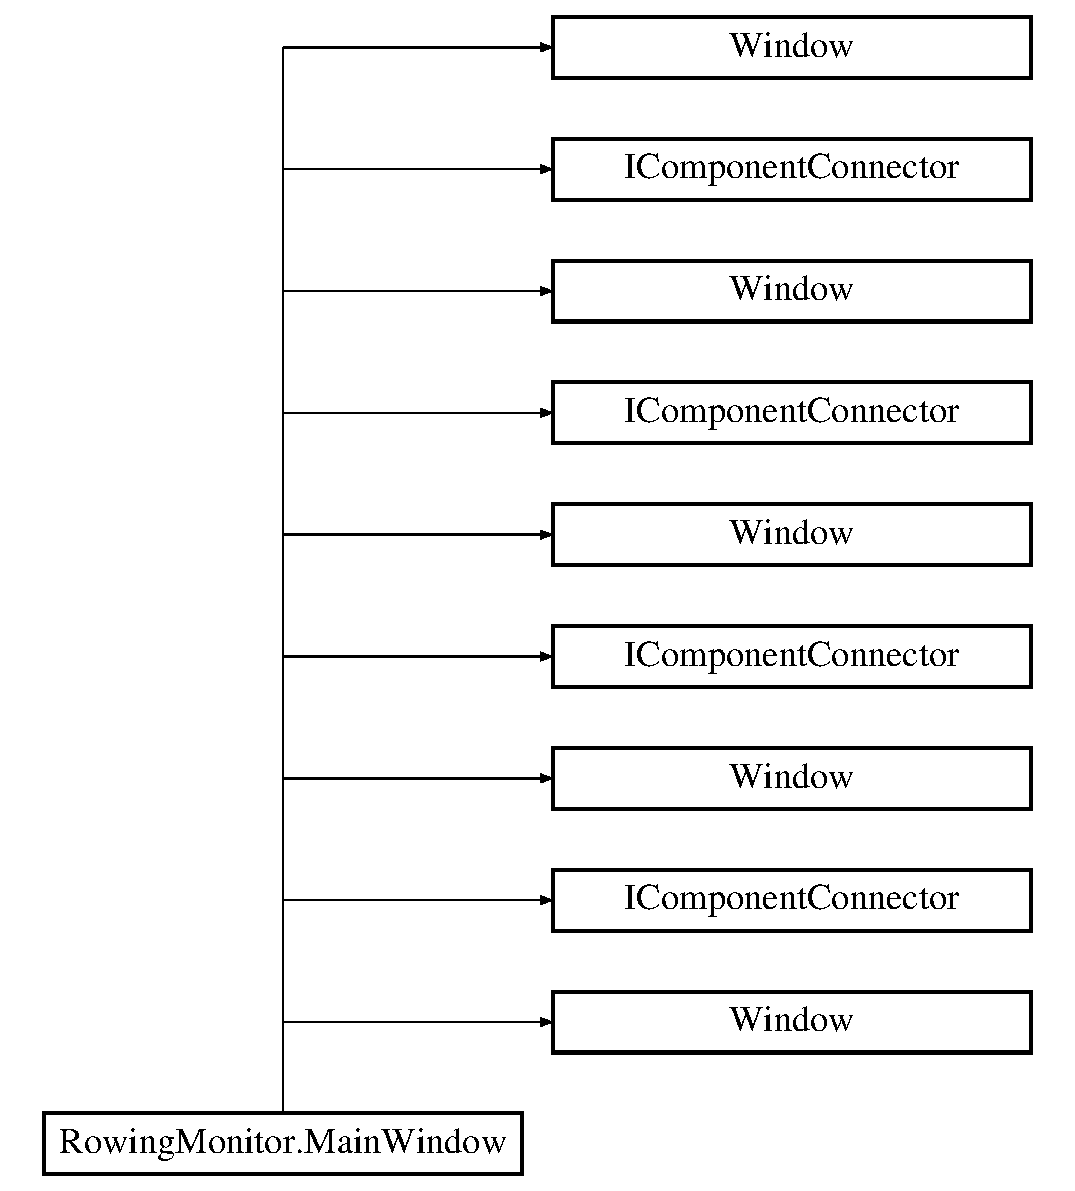
\includegraphics[height=9.000000cm]{class_rowing_monitor_1_1_main_window}
\end{center}
\end{figure}
\subsection*{Public Member Functions}
\begin{DoxyCompactItemize}
\item 
\hyperlink{class_rowing_monitor_1_1_main_window_aa33d7965b0fa09c32b1e7e2f782817d0}{Main\+Window} ()
\item 
void \hyperlink{class_rowing_monitor_1_1_main_window_afe76deea60e7fd9a534277f34037d22c}{Initialize\+Component} ()
\begin{DoxyCompactList}\small\item\em Initialize\+Component \end{DoxyCompactList}\item 
void \hyperlink{class_rowing_monitor_1_1_main_window_afe76deea60e7fd9a534277f34037d22c}{Initialize\+Component} ()
\begin{DoxyCompactList}\small\item\em Initialize\+Component \end{DoxyCompactList}\item 
void \hyperlink{class_rowing_monitor_1_1_main_window_afe76deea60e7fd9a534277f34037d22c}{Initialize\+Component} ()
\begin{DoxyCompactList}\small\item\em Initialize\+Component \end{DoxyCompactList}\item 
void \hyperlink{class_rowing_monitor_1_1_main_window_afe76deea60e7fd9a534277f34037d22c}{Initialize\+Component} ()
\begin{DoxyCompactList}\small\item\em Initialize\+Component \end{DoxyCompactList}\end{DoxyCompactItemize}


\subsection{Detailed Description}
Interaktionslogik für Main\+Window.\+xaml 

\hyperlink{class_rowing_monitor_1_1_main_window}{Main\+Window} 

\subsection{Constructor \& Destructor Documentation}
\mbox{\Hypertarget{class_rowing_monitor_1_1_main_window_aa33d7965b0fa09c32b1e7e2f782817d0}\label{class_rowing_monitor_1_1_main_window_aa33d7965b0fa09c32b1e7e2f782817d0}} 
\index{Rowing\+Monitor\+::\+Main\+Window@{Rowing\+Monitor\+::\+Main\+Window}!Main\+Window@{Main\+Window}}
\index{Main\+Window@{Main\+Window}!Rowing\+Monitor\+::\+Main\+Window@{Rowing\+Monitor\+::\+Main\+Window}}
\subsubsection{\texorpdfstring{Main\+Window()}{MainWindow()}}
{\footnotesize\ttfamily Rowing\+Monitor.\+Main\+Window.\+Main\+Window (\begin{DoxyParamCaption}{ }\end{DoxyParamCaption})}



\subsection{Member Function Documentation}
\mbox{\Hypertarget{class_rowing_monitor_1_1_main_window_afe76deea60e7fd9a534277f34037d22c}\label{class_rowing_monitor_1_1_main_window_afe76deea60e7fd9a534277f34037d22c}} 
\index{Rowing\+Monitor\+::\+Main\+Window@{Rowing\+Monitor\+::\+Main\+Window}!Initialize\+Component@{Initialize\+Component}}
\index{Initialize\+Component@{Initialize\+Component}!Rowing\+Monitor\+::\+Main\+Window@{Rowing\+Monitor\+::\+Main\+Window}}
\subsubsection{\texorpdfstring{Initialize\+Component()}{InitializeComponent()}\hspace{0.1cm}{\footnotesize\ttfamily [1/4]}}
{\footnotesize\ttfamily void Rowing\+Monitor.\+Main\+Window.\+Initialize\+Component (\begin{DoxyParamCaption}{ }\end{DoxyParamCaption})}



Initialize\+Component 

\mbox{\Hypertarget{class_rowing_monitor_1_1_main_window_afe76deea60e7fd9a534277f34037d22c}\label{class_rowing_monitor_1_1_main_window_afe76deea60e7fd9a534277f34037d22c}} 
\index{Rowing\+Monitor\+::\+Main\+Window@{Rowing\+Monitor\+::\+Main\+Window}!Initialize\+Component@{Initialize\+Component}}
\index{Initialize\+Component@{Initialize\+Component}!Rowing\+Monitor\+::\+Main\+Window@{Rowing\+Monitor\+::\+Main\+Window}}
\subsubsection{\texorpdfstring{Initialize\+Component()}{InitializeComponent()}\hspace{0.1cm}{\footnotesize\ttfamily [2/4]}}
{\footnotesize\ttfamily void Rowing\+Monitor.\+Main\+Window.\+Initialize\+Component (\begin{DoxyParamCaption}{ }\end{DoxyParamCaption})}



Initialize\+Component 

\mbox{\Hypertarget{class_rowing_monitor_1_1_main_window_afe76deea60e7fd9a534277f34037d22c}\label{class_rowing_monitor_1_1_main_window_afe76deea60e7fd9a534277f34037d22c}} 
\index{Rowing\+Monitor\+::\+Main\+Window@{Rowing\+Monitor\+::\+Main\+Window}!Initialize\+Component@{Initialize\+Component}}
\index{Initialize\+Component@{Initialize\+Component}!Rowing\+Monitor\+::\+Main\+Window@{Rowing\+Monitor\+::\+Main\+Window}}
\subsubsection{\texorpdfstring{Initialize\+Component()}{InitializeComponent()}\hspace{0.1cm}{\footnotesize\ttfamily [3/4]}}
{\footnotesize\ttfamily void Rowing\+Monitor.\+Main\+Window.\+Initialize\+Component (\begin{DoxyParamCaption}{ }\end{DoxyParamCaption})}



Initialize\+Component 

\mbox{\Hypertarget{class_rowing_monitor_1_1_main_window_afe76deea60e7fd9a534277f34037d22c}\label{class_rowing_monitor_1_1_main_window_afe76deea60e7fd9a534277f34037d22c}} 
\index{Rowing\+Monitor\+::\+Main\+Window@{Rowing\+Monitor\+::\+Main\+Window}!Initialize\+Component@{Initialize\+Component}}
\index{Initialize\+Component@{Initialize\+Component}!Rowing\+Monitor\+::\+Main\+Window@{Rowing\+Monitor\+::\+Main\+Window}}
\subsubsection{\texorpdfstring{Initialize\+Component()}{InitializeComponent()}\hspace{0.1cm}{\footnotesize\ttfamily [4/4]}}
{\footnotesize\ttfamily void Rowing\+Monitor.\+Main\+Window.\+Initialize\+Component (\begin{DoxyParamCaption}{ }\end{DoxyParamCaption})}



Initialize\+Component 



The documentation for this class was generated from the following files\+:\begin{DoxyCompactItemize}
\item 
\hyperlink{_main_window_8xaml_8cs}{Main\+Window.\+xaml.\+cs}\item 
obj/\+Debug/\hyperlink{_debug_2_main_window_8g_8cs}{Main\+Window.\+g.\+cs}\item 
obj/\+Debug/\hyperlink{_debug_2_main_window_8g_8i_8cs}{Main\+Window.\+g.\+i.\+cs}\end{DoxyCompactItemize}

\hypertarget{class_rowing_monitor_1_1_model_1_1_one_euro_filter_smoothing}{}\section{Rowing\+Monitor.\+Model.\+One\+Euro\+Filter\+Smoothing Class Reference}
\label{class_rowing_monitor_1_1_model_1_1_one_euro_filter_smoothing}\index{Rowing\+Monitor.\+Model.\+One\+Euro\+Filter\+Smoothing@{Rowing\+Monitor.\+Model.\+One\+Euro\+Filter\+Smoothing}}
\subsection*{Public Member Functions}
\begin{DoxyCompactItemize}
\item 
delegate void \hyperlink{class_rowing_monitor_1_1_model_1_1_one_euro_filter_smoothing_a22becc35eb5432a3a90b8e61d5c8171f}{Smoothed\+Frame\+Arrived\+Event\+Handler} (Object sender, \hyperlink{class_rowing_monitor_1_1_model_1_1_smoothed_frame_arrived_event_args}{Smoothed\+Frame\+Arrived\+Event\+Args} e)
\item 
\hyperlink{class_rowing_monitor_1_1_model_1_1_one_euro_filter_smoothing_a1c3c89d4e59552370c5c0d56edac8a19}{One\+Euro\+Filter\+Smoothing} ()
\item 
void \hyperlink{class_rowing_monitor_1_1_model_1_1_one_euro_filter_smoothing_a2dcb40fcf4cd02302a23f421f710ac8c}{Update\+Filter} (\hyperlink{struct_rowing_monitor_1_1_model_1_1_util_1_1_joint_data}{Joint\+Data} joint\+Data)
\end{DoxyCompactItemize}
\subsection*{Static Public Member Functions}
\begin{DoxyCompactItemize}
\item 
static Dictionary$<$ Joint\+Type, Dictionary$<$ String, Double $>$ $>$ \hyperlink{class_rowing_monitor_1_1_model_1_1_one_euro_filter_smoothing_ab5e23859c5dbb67cdafebec5fea702f5}{Init\+Cutoff\+Dictionary} (Double value)
\begin{DoxyCompactList}\small\item\em Initliazies a dictionary of all joint types with a given value. \end{DoxyCompactList}\end{DoxyCompactItemize}
\subsection*{Properties}
\begin{DoxyCompactItemize}
\item 
Double \hyperlink{class_rowing_monitor_1_1_model_1_1_one_euro_filter_smoothing_abbe908f1d7748febfc27336f42b95a6f}{Beta}\hspace{0.3cm}{\ttfamily  \mbox{[}get, set\mbox{]}}
\item 
double \hyperlink{class_rowing_monitor_1_1_model_1_1_one_euro_filter_smoothing_ada991e92f7ecbde83ab171a585f6d6d2}{Fcmin}\hspace{0.3cm}{\ttfamily  \mbox{[}get, set\mbox{]}}
\item 
Dictionary$<$ Joint\+Type, Dictionary$<$ string, double $>$ $>$ \hyperlink{class_rowing_monitor_1_1_model_1_1_one_euro_filter_smoothing_a9763ac7c63ca0ad07c8a0a00f645a9fc}{Mincutoff}\hspace{0.3cm}{\ttfamily  \mbox{[}get, set\mbox{]}}
\end{DoxyCompactItemize}
\subsection*{Events}
\begin{DoxyCompactItemize}
\item 
\hyperlink{class_rowing_monitor_1_1_model_1_1_one_euro_filter_smoothing_a22becc35eb5432a3a90b8e61d5c8171f}{Smoothed\+Frame\+Arrived\+Event\+Handler} \hyperlink{class_rowing_monitor_1_1_model_1_1_one_euro_filter_smoothing_ad6eddf578afaace11e6d1f1a74ff018a}{Smoothed\+Frame\+Arrived}
\end{DoxyCompactItemize}


\subsection{Constructor \& Destructor Documentation}
\mbox{\Hypertarget{class_rowing_monitor_1_1_model_1_1_one_euro_filter_smoothing_a1c3c89d4e59552370c5c0d56edac8a19}\label{class_rowing_monitor_1_1_model_1_1_one_euro_filter_smoothing_a1c3c89d4e59552370c5c0d56edac8a19}} 
\index{Rowing\+Monitor\+::\+Model\+::\+One\+Euro\+Filter\+Smoothing@{Rowing\+Monitor\+::\+Model\+::\+One\+Euro\+Filter\+Smoothing}!One\+Euro\+Filter\+Smoothing@{One\+Euro\+Filter\+Smoothing}}
\index{One\+Euro\+Filter\+Smoothing@{One\+Euro\+Filter\+Smoothing}!Rowing\+Monitor\+::\+Model\+::\+One\+Euro\+Filter\+Smoothing@{Rowing\+Monitor\+::\+Model\+::\+One\+Euro\+Filter\+Smoothing}}
\subsubsection{\texorpdfstring{One\+Euro\+Filter\+Smoothing()}{OneEuroFilterSmoothing()}}
{\footnotesize\ttfamily Rowing\+Monitor.\+Model.\+One\+Euro\+Filter\+Smoothing.\+One\+Euro\+Filter\+Smoothing (\begin{DoxyParamCaption}{ }\end{DoxyParamCaption})}



\subsection{Member Function Documentation}
\mbox{\Hypertarget{class_rowing_monitor_1_1_model_1_1_one_euro_filter_smoothing_ab5e23859c5dbb67cdafebec5fea702f5}\label{class_rowing_monitor_1_1_model_1_1_one_euro_filter_smoothing_ab5e23859c5dbb67cdafebec5fea702f5}} 
\index{Rowing\+Monitor\+::\+Model\+::\+One\+Euro\+Filter\+Smoothing@{Rowing\+Monitor\+::\+Model\+::\+One\+Euro\+Filter\+Smoothing}!Init\+Cutoff\+Dictionary@{Init\+Cutoff\+Dictionary}}
\index{Init\+Cutoff\+Dictionary@{Init\+Cutoff\+Dictionary}!Rowing\+Monitor\+::\+Model\+::\+One\+Euro\+Filter\+Smoothing@{Rowing\+Monitor\+::\+Model\+::\+One\+Euro\+Filter\+Smoothing}}
\subsubsection{\texorpdfstring{Init\+Cutoff\+Dictionary()}{InitCutoffDictionary()}}
{\footnotesize\ttfamily static Dictionary$<$Joint\+Type, Dictionary$<$String, Double$>$ $>$ Rowing\+Monitor.\+Model.\+One\+Euro\+Filter\+Smoothing.\+Init\+Cutoff\+Dictionary (\begin{DoxyParamCaption}\item[{Double}]{value }\end{DoxyParamCaption})\hspace{0.3cm}{\ttfamily [static]}}



Initliazies a dictionary of all joint types with a given value. 


\begin{DoxyParams}{Parameters}
{\em value} & \\
\hline
\end{DoxyParams}
\begin{DoxyReturn}{Returns}

\end{DoxyReturn}
\mbox{\Hypertarget{class_rowing_monitor_1_1_model_1_1_one_euro_filter_smoothing_a22becc35eb5432a3a90b8e61d5c8171f}\label{class_rowing_monitor_1_1_model_1_1_one_euro_filter_smoothing_a22becc35eb5432a3a90b8e61d5c8171f}} 
\index{Rowing\+Monitor\+::\+Model\+::\+One\+Euro\+Filter\+Smoothing@{Rowing\+Monitor\+::\+Model\+::\+One\+Euro\+Filter\+Smoothing}!Smoothed\+Frame\+Arrived\+Event\+Handler@{Smoothed\+Frame\+Arrived\+Event\+Handler}}
\index{Smoothed\+Frame\+Arrived\+Event\+Handler@{Smoothed\+Frame\+Arrived\+Event\+Handler}!Rowing\+Monitor\+::\+Model\+::\+One\+Euro\+Filter\+Smoothing@{Rowing\+Monitor\+::\+Model\+::\+One\+Euro\+Filter\+Smoothing}}
\subsubsection{\texorpdfstring{Smoothed\+Frame\+Arrived\+Event\+Handler()}{SmoothedFrameArrivedEventHandler()}}
{\footnotesize\ttfamily delegate void Rowing\+Monitor.\+Model.\+One\+Euro\+Filter\+Smoothing.\+Smoothed\+Frame\+Arrived\+Event\+Handler (\begin{DoxyParamCaption}\item[{Object}]{sender,  }\item[{\hyperlink{class_rowing_monitor_1_1_model_1_1_smoothed_frame_arrived_event_args}{Smoothed\+Frame\+Arrived\+Event\+Args}}]{e }\end{DoxyParamCaption})}

\mbox{\Hypertarget{class_rowing_monitor_1_1_model_1_1_one_euro_filter_smoothing_a2dcb40fcf4cd02302a23f421f710ac8c}\label{class_rowing_monitor_1_1_model_1_1_one_euro_filter_smoothing_a2dcb40fcf4cd02302a23f421f710ac8c}} 
\index{Rowing\+Monitor\+::\+Model\+::\+One\+Euro\+Filter\+Smoothing@{Rowing\+Monitor\+::\+Model\+::\+One\+Euro\+Filter\+Smoothing}!Update\+Filter@{Update\+Filter}}
\index{Update\+Filter@{Update\+Filter}!Rowing\+Monitor\+::\+Model\+::\+One\+Euro\+Filter\+Smoothing@{Rowing\+Monitor\+::\+Model\+::\+One\+Euro\+Filter\+Smoothing}}
\subsubsection{\texorpdfstring{Update\+Filter()}{UpdateFilter()}}
{\footnotesize\ttfamily void Rowing\+Monitor.\+Model.\+One\+Euro\+Filter\+Smoothing.\+Update\+Filter (\begin{DoxyParamCaption}\item[{\hyperlink{struct_rowing_monitor_1_1_model_1_1_util_1_1_joint_data}{Joint\+Data}}]{joint\+Data }\end{DoxyParamCaption})}



\subsection{Property Documentation}
\mbox{\Hypertarget{class_rowing_monitor_1_1_model_1_1_one_euro_filter_smoothing_abbe908f1d7748febfc27336f42b95a6f}\label{class_rowing_monitor_1_1_model_1_1_one_euro_filter_smoothing_abbe908f1d7748febfc27336f42b95a6f}} 
\index{Rowing\+Monitor\+::\+Model\+::\+One\+Euro\+Filter\+Smoothing@{Rowing\+Monitor\+::\+Model\+::\+One\+Euro\+Filter\+Smoothing}!Beta@{Beta}}
\index{Beta@{Beta}!Rowing\+Monitor\+::\+Model\+::\+One\+Euro\+Filter\+Smoothing@{Rowing\+Monitor\+::\+Model\+::\+One\+Euro\+Filter\+Smoothing}}
\subsubsection{\texorpdfstring{Beta}{Beta}}
{\footnotesize\ttfamily Double Rowing\+Monitor.\+Model.\+One\+Euro\+Filter\+Smoothing.\+Beta\hspace{0.3cm}{\ttfamily [get]}, {\ttfamily [set]}}

\mbox{\Hypertarget{class_rowing_monitor_1_1_model_1_1_one_euro_filter_smoothing_ada991e92f7ecbde83ab171a585f6d6d2}\label{class_rowing_monitor_1_1_model_1_1_one_euro_filter_smoothing_ada991e92f7ecbde83ab171a585f6d6d2}} 
\index{Rowing\+Monitor\+::\+Model\+::\+One\+Euro\+Filter\+Smoothing@{Rowing\+Monitor\+::\+Model\+::\+One\+Euro\+Filter\+Smoothing}!Fcmin@{Fcmin}}
\index{Fcmin@{Fcmin}!Rowing\+Monitor\+::\+Model\+::\+One\+Euro\+Filter\+Smoothing@{Rowing\+Monitor\+::\+Model\+::\+One\+Euro\+Filter\+Smoothing}}
\subsubsection{\texorpdfstring{Fcmin}{Fcmin}}
{\footnotesize\ttfamily double Rowing\+Monitor.\+Model.\+One\+Euro\+Filter\+Smoothing.\+Fcmin\hspace{0.3cm}{\ttfamily [get]}, {\ttfamily [set]}}

\mbox{\Hypertarget{class_rowing_monitor_1_1_model_1_1_one_euro_filter_smoothing_a9763ac7c63ca0ad07c8a0a00f645a9fc}\label{class_rowing_monitor_1_1_model_1_1_one_euro_filter_smoothing_a9763ac7c63ca0ad07c8a0a00f645a9fc}} 
\index{Rowing\+Monitor\+::\+Model\+::\+One\+Euro\+Filter\+Smoothing@{Rowing\+Monitor\+::\+Model\+::\+One\+Euro\+Filter\+Smoothing}!Mincutoff@{Mincutoff}}
\index{Mincutoff@{Mincutoff}!Rowing\+Monitor\+::\+Model\+::\+One\+Euro\+Filter\+Smoothing@{Rowing\+Monitor\+::\+Model\+::\+One\+Euro\+Filter\+Smoothing}}
\subsubsection{\texorpdfstring{Mincutoff}{Mincutoff}}
{\footnotesize\ttfamily Dictionary$<$Joint\+Type, Dictionary$<$string, double$>$ $>$ Rowing\+Monitor.\+Model.\+One\+Euro\+Filter\+Smoothing.\+Mincutoff\hspace{0.3cm}{\ttfamily [get]}, {\ttfamily [set]}}



\subsection{Event Documentation}
\mbox{\Hypertarget{class_rowing_monitor_1_1_model_1_1_one_euro_filter_smoothing_ad6eddf578afaace11e6d1f1a74ff018a}\label{class_rowing_monitor_1_1_model_1_1_one_euro_filter_smoothing_ad6eddf578afaace11e6d1f1a74ff018a}} 
\index{Rowing\+Monitor\+::\+Model\+::\+One\+Euro\+Filter\+Smoothing@{Rowing\+Monitor\+::\+Model\+::\+One\+Euro\+Filter\+Smoothing}!Smoothed\+Frame\+Arrived@{Smoothed\+Frame\+Arrived}}
\index{Smoothed\+Frame\+Arrived@{Smoothed\+Frame\+Arrived}!Rowing\+Monitor\+::\+Model\+::\+One\+Euro\+Filter\+Smoothing@{Rowing\+Monitor\+::\+Model\+::\+One\+Euro\+Filter\+Smoothing}}
\subsubsection{\texorpdfstring{Smoothed\+Frame\+Arrived}{SmoothedFrameArrived}}
{\footnotesize\ttfamily \hyperlink{class_rowing_monitor_1_1_model_1_1_one_euro_filter_smoothing_a22becc35eb5432a3a90b8e61d5c8171f}{Smoothed\+Frame\+Arrived\+Event\+Handler} Rowing\+Monitor.\+Model.\+One\+Euro\+Filter\+Smoothing.\+Smoothed\+Frame\+Arrived}



The documentation for this class was generated from the following file\+:\begin{DoxyCompactItemize}
\item 
Model/\+Pipeline/\hyperlink{_one_euro_filter_smoothing_8cs}{One\+Euro\+Filter\+Smoothing.\+cs}\end{DoxyCompactItemize}

\hypertarget{class_rowing_monitor_1_1_model_1_1_plot}{}\section{Rowing\+Monitor.\+Model.\+Plot Class Reference}
\label{class_rowing_monitor_1_1_model_1_1_plot}\index{Rowing\+Monitor.\+Model.\+Plot@{Rowing\+Monitor.\+Model.\+Plot}}
\subsection*{Public Member Functions}
\begin{DoxyCompactItemize}
\item 
\hyperlink{class_rowing_monitor_1_1_model_1_1_plot_a950ad596730f1ff80a5998f16a4c0d3c}{Plot} ()
\begin{DoxyCompactList}\small\item\em Creates a plot for the view. \end{DoxyCompactList}\item 
\hyperlink{class_rowing_monitor_1_1_model_1_1_plot_a12760bee76f583deb2741bc223be33e2}{Plot} (float range)
\begin{DoxyCompactList}\small\item\em Creates a plot for the view. \end{DoxyCompactList}\item 
void \hyperlink{class_rowing_monitor_1_1_model_1_1_plot_a8adb8a568e1c387863ec524633008d36}{Update\+Plot} (Dictionary$<$ String, List$<$ \hyperlink{struct_rowing_monitor_1_1_model_1_1_plot_data}{Plot\+Data} $>$$>$ data\+Points, String title, Dictionary$<$ String, Oxy\+Color $>$ colors=null)
\begin{DoxyCompactList}\small\item\em Draws a plot of given data points. \end{DoxyCompactList}\item 
void \hyperlink{class_rowing_monitor_1_1_model_1_1_plot_a408af0095ce2ead5b7d897915a378340}{Init} (String title, Dictionary$<$ String, Oxy\+Color $>$ colors=null)
\item 
void \hyperlink{class_rowing_monitor_1_1_model_1_1_plot_a7502c1cc303bfefb6de6b08efb874b1b}{Add\+Data\+Point} (string series, double\mbox{[}$\,$\mbox{]} values)
\end{DoxyCompactItemize}
\subsection*{Properties}
\begin{DoxyCompactItemize}
\item 
Plot\+Model \hyperlink{class_rowing_monitor_1_1_model_1_1_plot_a702a4f703d9a9452dade1f19e91fc7a4}{Plot\+Model}\hspace{0.3cm}{\ttfamily  \mbox{[}get\mbox{]}}
\item 
Dictionary$<$ string, Oxy\+Color $>$ \hyperlink{class_rowing_monitor_1_1_model_1_1_plot_af5c811e7e98de0927650caede84921a5}{Colors}\hspace{0.3cm}{\ttfamily  \mbox{[}get, set\mbox{]}}
\end{DoxyCompactItemize}


\subsection{Constructor \& Destructor Documentation}
\mbox{\Hypertarget{class_rowing_monitor_1_1_model_1_1_plot_a950ad596730f1ff80a5998f16a4c0d3c}\label{class_rowing_monitor_1_1_model_1_1_plot_a950ad596730f1ff80a5998f16a4c0d3c}} 
\index{Rowing\+Monitor\+::\+Model\+::\+Plot@{Rowing\+Monitor\+::\+Model\+::\+Plot}!Plot@{Plot}}
\index{Plot@{Plot}!Rowing\+Monitor\+::\+Model\+::\+Plot@{Rowing\+Monitor\+::\+Model\+::\+Plot}}
\subsubsection{\texorpdfstring{Plot()}{Plot()}\hspace{0.1cm}{\footnotesize\ttfamily [1/2]}}
{\footnotesize\ttfamily Rowing\+Monitor.\+Model.\+Plot.\+Plot (\begin{DoxyParamCaption}{ }\end{DoxyParamCaption})}



Creates a plot for the view. 

\mbox{\Hypertarget{class_rowing_monitor_1_1_model_1_1_plot_a12760bee76f583deb2741bc223be33e2}\label{class_rowing_monitor_1_1_model_1_1_plot_a12760bee76f583deb2741bc223be33e2}} 
\index{Rowing\+Monitor\+::\+Model\+::\+Plot@{Rowing\+Monitor\+::\+Model\+::\+Plot}!Plot@{Plot}}
\index{Plot@{Plot}!Rowing\+Monitor\+::\+Model\+::\+Plot@{Rowing\+Monitor\+::\+Model\+::\+Plot}}
\subsubsection{\texorpdfstring{Plot()}{Plot()}\hspace{0.1cm}{\footnotesize\ttfamily [2/2]}}
{\footnotesize\ttfamily Rowing\+Monitor.\+Model.\+Plot.\+Plot (\begin{DoxyParamCaption}\item[{float}]{range }\end{DoxyParamCaption})}



Creates a plot for the view. 

If the number data points for one line series reaches the max threshold, all older data points will not be shown. 


\begin{DoxyParams}{Parameters}
{\em range} & Range of values along the x axis.\\
\hline
\end{DoxyParams}


\subsection{Member Function Documentation}
\mbox{\Hypertarget{class_rowing_monitor_1_1_model_1_1_plot_a7502c1cc303bfefb6de6b08efb874b1b}\label{class_rowing_monitor_1_1_model_1_1_plot_a7502c1cc303bfefb6de6b08efb874b1b}} 
\index{Rowing\+Monitor\+::\+Model\+::\+Plot@{Rowing\+Monitor\+::\+Model\+::\+Plot}!Add\+Data\+Point@{Add\+Data\+Point}}
\index{Add\+Data\+Point@{Add\+Data\+Point}!Rowing\+Monitor\+::\+Model\+::\+Plot@{Rowing\+Monitor\+::\+Model\+::\+Plot}}
\subsubsection{\texorpdfstring{Add\+Data\+Point()}{AddDataPoint()}}
{\footnotesize\ttfamily void Rowing\+Monitor.\+Model.\+Plot.\+Add\+Data\+Point (\begin{DoxyParamCaption}\item[{string}]{series,  }\item[{double \mbox{[}$\,$\mbox{]}}]{values }\end{DoxyParamCaption})}

\mbox{\Hypertarget{class_rowing_monitor_1_1_model_1_1_plot_a408af0095ce2ead5b7d897915a378340}\label{class_rowing_monitor_1_1_model_1_1_plot_a408af0095ce2ead5b7d897915a378340}} 
\index{Rowing\+Monitor\+::\+Model\+::\+Plot@{Rowing\+Monitor\+::\+Model\+::\+Plot}!Init@{Init}}
\index{Init@{Init}!Rowing\+Monitor\+::\+Model\+::\+Plot@{Rowing\+Monitor\+::\+Model\+::\+Plot}}
\subsubsection{\texorpdfstring{Init()}{Init()}}
{\footnotesize\ttfamily void Rowing\+Monitor.\+Model.\+Plot.\+Init (\begin{DoxyParamCaption}\item[{String}]{title,  }\item[{Dictionary$<$ String, Oxy\+Color $>$}]{colors = {\ttfamily null} }\end{DoxyParamCaption})}

\mbox{\Hypertarget{class_rowing_monitor_1_1_model_1_1_plot_a8adb8a568e1c387863ec524633008d36}\label{class_rowing_monitor_1_1_model_1_1_plot_a8adb8a568e1c387863ec524633008d36}} 
\index{Rowing\+Monitor\+::\+Model\+::\+Plot@{Rowing\+Monitor\+::\+Model\+::\+Plot}!Update\+Plot@{Update\+Plot}}
\index{Update\+Plot@{Update\+Plot}!Rowing\+Monitor\+::\+Model\+::\+Plot@{Rowing\+Monitor\+::\+Model\+::\+Plot}}
\subsubsection{\texorpdfstring{Update\+Plot()}{UpdatePlot()}}
{\footnotesize\ttfamily void Rowing\+Monitor.\+Model.\+Plot.\+Update\+Plot (\begin{DoxyParamCaption}\item[{Dictionary$<$ String, List$<$ \hyperlink{struct_rowing_monitor_1_1_model_1_1_plot_data}{Plot\+Data} $>$$>$}]{data\+Points,  }\item[{String}]{title,  }\item[{Dictionary$<$ String, Oxy\+Color $>$}]{colors = {\ttfamily null} }\end{DoxyParamCaption})}



Draws a plot of given data points. 

The Raise\+Property\+Changed event must be raised after the update to refresh the plot view. 


\begin{DoxyParams}{Parameters}
{\em data\+Points} & Set of data points (x,y). The Key will be used as title of the line series.\\
\hline
{\em title} & Title of the plot.\\
\hline
\end{DoxyParams}


\subsection{Property Documentation}
\mbox{\Hypertarget{class_rowing_monitor_1_1_model_1_1_plot_af5c811e7e98de0927650caede84921a5}\label{class_rowing_monitor_1_1_model_1_1_plot_af5c811e7e98de0927650caede84921a5}} 
\index{Rowing\+Monitor\+::\+Model\+::\+Plot@{Rowing\+Monitor\+::\+Model\+::\+Plot}!Colors@{Colors}}
\index{Colors@{Colors}!Rowing\+Monitor\+::\+Model\+::\+Plot@{Rowing\+Monitor\+::\+Model\+::\+Plot}}
\subsubsection{\texorpdfstring{Colors}{Colors}}
{\footnotesize\ttfamily Dictionary$<$string, Oxy\+Color$>$ Rowing\+Monitor.\+Model.\+Plot.\+Colors\hspace{0.3cm}{\ttfamily [get]}, {\ttfamily [set]}}

\mbox{\Hypertarget{class_rowing_monitor_1_1_model_1_1_plot_a702a4f703d9a9452dade1f19e91fc7a4}\label{class_rowing_monitor_1_1_model_1_1_plot_a702a4f703d9a9452dade1f19e91fc7a4}} 
\index{Rowing\+Monitor\+::\+Model\+::\+Plot@{Rowing\+Monitor\+::\+Model\+::\+Plot}!Plot\+Model@{Plot\+Model}}
\index{Plot\+Model@{Plot\+Model}!Rowing\+Monitor\+::\+Model\+::\+Plot@{Rowing\+Monitor\+::\+Model\+::\+Plot}}
\subsubsection{\texorpdfstring{Plot\+Model}{PlotModel}}
{\footnotesize\ttfamily Plot\+Model Rowing\+Monitor.\+Model.\+Plot.\+Plot\+Model\hspace{0.3cm}{\ttfamily [get]}}



The documentation for this class was generated from the following file\+:\begin{DoxyCompactItemize}
\item 
Model/\+Pipeline/\hyperlink{_plot_8cs}{Plot.\+cs}\end{DoxyCompactItemize}

\hypertarget{struct_rowing_monitor_1_1_model_1_1_plot_data}{}\section{Rowing\+Monitor.\+Model.\+Plot\+Data Struct Reference}
\label{struct_rowing_monitor_1_1_model_1_1_plot_data}\index{Rowing\+Monitor.\+Model.\+Plot\+Data@{Rowing\+Monitor.\+Model.\+Plot\+Data}}
\subsection*{Properties}
\begin{DoxyCompactItemize}
\item 
double \hyperlink{struct_rowing_monitor_1_1_model_1_1_plot_data_a0e4ce74a471cf5ffbc621bcc18e6ceb8}{X}\hspace{0.3cm}{\ttfamily  \mbox{[}get, set\mbox{]}}
\item 
double \hyperlink{struct_rowing_monitor_1_1_model_1_1_plot_data_aed25da377c94a8a3a8684623119b11e6}{Y}\hspace{0.3cm}{\ttfamily  \mbox{[}get, set\mbox{]}}
\item 
string \hyperlink{struct_rowing_monitor_1_1_model_1_1_plot_data_a8340e2244b7b59bc7949dda192a8c99a}{Annotation}\hspace{0.3cm}{\ttfamily  \mbox{[}get, set\mbox{]}}
\item 
\hyperlink{namespace_rowing_monitor_1_1_model_1_1_util_a01e1a06061533b246feb7421c9d0107f}{Data\+Stream\+Type} \hyperlink{struct_rowing_monitor_1_1_model_1_1_plot_data_a254e431007698194e2a440cba5fc48a5}{Data\+Stream\+Type}\hspace{0.3cm}{\ttfamily  \mbox{[}get, set\mbox{]}}
\end{DoxyCompactItemize}


\subsection{Property Documentation}
\mbox{\Hypertarget{struct_rowing_monitor_1_1_model_1_1_plot_data_a8340e2244b7b59bc7949dda192a8c99a}\label{struct_rowing_monitor_1_1_model_1_1_plot_data_a8340e2244b7b59bc7949dda192a8c99a}} 
\index{Rowing\+Monitor\+::\+Model\+::\+Plot\+Data@{Rowing\+Monitor\+::\+Model\+::\+Plot\+Data}!Annotation@{Annotation}}
\index{Annotation@{Annotation}!Rowing\+Monitor\+::\+Model\+::\+Plot\+Data@{Rowing\+Monitor\+::\+Model\+::\+Plot\+Data}}
\subsubsection{\texorpdfstring{Annotation}{Annotation}}
{\footnotesize\ttfamily string Rowing\+Monitor.\+Model.\+Plot\+Data.\+Annotation\hspace{0.3cm}{\ttfamily [get]}, {\ttfamily [set]}}

\mbox{\Hypertarget{struct_rowing_monitor_1_1_model_1_1_plot_data_a254e431007698194e2a440cba5fc48a5}\label{struct_rowing_monitor_1_1_model_1_1_plot_data_a254e431007698194e2a440cba5fc48a5}} 
\index{Rowing\+Monitor\+::\+Model\+::\+Plot\+Data@{Rowing\+Monitor\+::\+Model\+::\+Plot\+Data}!Data\+Stream\+Type@{Data\+Stream\+Type}}
\index{Data\+Stream\+Type@{Data\+Stream\+Type}!Rowing\+Monitor\+::\+Model\+::\+Plot\+Data@{Rowing\+Monitor\+::\+Model\+::\+Plot\+Data}}
\subsubsection{\texorpdfstring{Data\+Stream\+Type}{DataStreamType}}
{\footnotesize\ttfamily \hyperlink{namespace_rowing_monitor_1_1_model_1_1_util_a01e1a06061533b246feb7421c9d0107f}{Data\+Stream\+Type} Rowing\+Monitor.\+Model.\+Plot\+Data.\+Data\+Stream\+Type\hspace{0.3cm}{\ttfamily [get]}, {\ttfamily [set]}}

\mbox{\Hypertarget{struct_rowing_monitor_1_1_model_1_1_plot_data_a0e4ce74a471cf5ffbc621bcc18e6ceb8}\label{struct_rowing_monitor_1_1_model_1_1_plot_data_a0e4ce74a471cf5ffbc621bcc18e6ceb8}} 
\index{Rowing\+Monitor\+::\+Model\+::\+Plot\+Data@{Rowing\+Monitor\+::\+Model\+::\+Plot\+Data}!X@{X}}
\index{X@{X}!Rowing\+Monitor\+::\+Model\+::\+Plot\+Data@{Rowing\+Monitor\+::\+Model\+::\+Plot\+Data}}
\subsubsection{\texorpdfstring{X}{X}}
{\footnotesize\ttfamily double Rowing\+Monitor.\+Model.\+Plot\+Data.\+X\hspace{0.3cm}{\ttfamily [get]}, {\ttfamily [set]}}

\mbox{\Hypertarget{struct_rowing_monitor_1_1_model_1_1_plot_data_aed25da377c94a8a3a8684623119b11e6}\label{struct_rowing_monitor_1_1_model_1_1_plot_data_aed25da377c94a8a3a8684623119b11e6}} 
\index{Rowing\+Monitor\+::\+Model\+::\+Plot\+Data@{Rowing\+Monitor\+::\+Model\+::\+Plot\+Data}!Y@{Y}}
\index{Y@{Y}!Rowing\+Monitor\+::\+Model\+::\+Plot\+Data@{Rowing\+Monitor\+::\+Model\+::\+Plot\+Data}}
\subsubsection{\texorpdfstring{Y}{Y}}
{\footnotesize\ttfamily double Rowing\+Monitor.\+Model.\+Plot\+Data.\+Y\hspace{0.3cm}{\ttfamily [get]}, {\ttfamily [set]}}



The documentation for this struct was generated from the following file\+:\begin{DoxyCompactItemize}
\item 
Model/\+Pipeline/\hyperlink{_plot_8cs}{Plot.\+cs}\end{DoxyCompactItemize}

\hypertarget{class_rowing_monitor_1_1_relay_command}{}\section{Rowing\+Monitor.\+Relay\+Command Class Reference}
\label{class_rowing_monitor_1_1_relay_command}\index{Rowing\+Monitor.\+Relay\+Command@{Rowing\+Monitor.\+Relay\+Command}}
Inheritance diagram for Rowing\+Monitor.\+Relay\+Command\+:\begin{figure}[H]
\begin{center}
\leavevmode
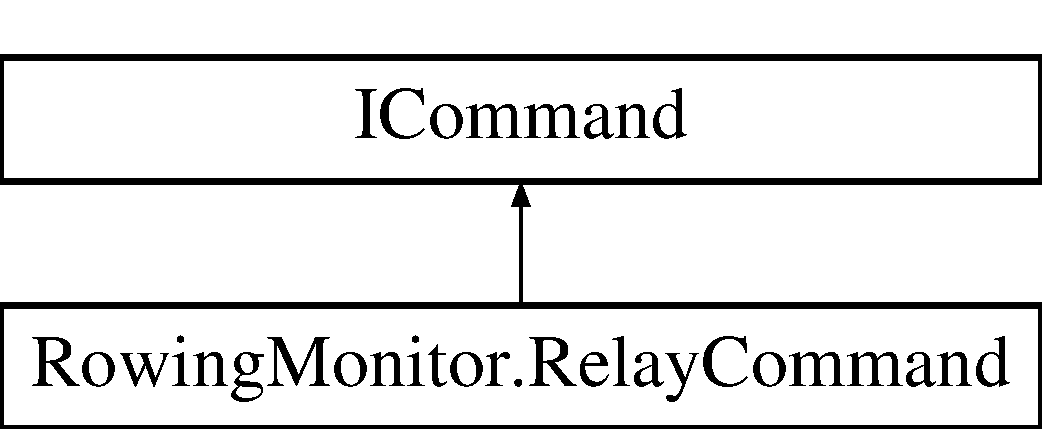
\includegraphics[height=2.000000cm]{class_rowing_monitor_1_1_relay_command}
\end{center}
\end{figure}
\subsection*{Public Member Functions}
\begin{DoxyCompactItemize}
\item 
\hyperlink{class_rowing_monitor_1_1_relay_command_a489257b2b64ff595ac8cf6f4dea07822}{Relay\+Command} (Action$<$ object $>$ execute)
\item 
\hyperlink{class_rowing_monitor_1_1_relay_command_a683db6291fb9d78a125cff700be862d6}{Relay\+Command} (Action$<$ object $>$ execute, Predicate$<$ object $>$ can\+Execute)
\item 
void \hyperlink{class_rowing_monitor_1_1_relay_command_ac4ca734c8e04bfb87cf1a1c295fb2d5b}{Execute} (object parameter)
\item 
bool \hyperlink{class_rowing_monitor_1_1_relay_command_a85fe9d9b44a1db38da8e1330d6715b30}{Can\+Execute} (object parameter)
\end{DoxyCompactItemize}
\subsection*{Properties}
\begin{DoxyCompactItemize}
\item 
Event\+Handler \hyperlink{class_rowing_monitor_1_1_relay_command_ae4dd035ea91a110089885a49c15fa525}{Can\+Execute\+Changed}
\end{DoxyCompactItemize}


\subsection{Constructor \& Destructor Documentation}
\mbox{\Hypertarget{class_rowing_monitor_1_1_relay_command_a489257b2b64ff595ac8cf6f4dea07822}\label{class_rowing_monitor_1_1_relay_command_a489257b2b64ff595ac8cf6f4dea07822}} 
\index{Rowing\+Monitor\+::\+Relay\+Command@{Rowing\+Monitor\+::\+Relay\+Command}!Relay\+Command@{Relay\+Command}}
\index{Relay\+Command@{Relay\+Command}!Rowing\+Monitor\+::\+Relay\+Command@{Rowing\+Monitor\+::\+Relay\+Command}}
\subsubsection{\texorpdfstring{Relay\+Command()}{RelayCommand()}\hspace{0.1cm}{\footnotesize\ttfamily [1/2]}}
{\footnotesize\ttfamily Rowing\+Monitor.\+Relay\+Command.\+Relay\+Command (\begin{DoxyParamCaption}\item[{Action$<$ object $>$}]{execute }\end{DoxyParamCaption})}

\mbox{\Hypertarget{class_rowing_monitor_1_1_relay_command_a683db6291fb9d78a125cff700be862d6}\label{class_rowing_monitor_1_1_relay_command_a683db6291fb9d78a125cff700be862d6}} 
\index{Rowing\+Monitor\+::\+Relay\+Command@{Rowing\+Monitor\+::\+Relay\+Command}!Relay\+Command@{Relay\+Command}}
\index{Relay\+Command@{Relay\+Command}!Rowing\+Monitor\+::\+Relay\+Command@{Rowing\+Monitor\+::\+Relay\+Command}}
\subsubsection{\texorpdfstring{Relay\+Command()}{RelayCommand()}\hspace{0.1cm}{\footnotesize\ttfamily [2/2]}}
{\footnotesize\ttfamily Rowing\+Monitor.\+Relay\+Command.\+Relay\+Command (\begin{DoxyParamCaption}\item[{Action$<$ object $>$}]{execute,  }\item[{Predicate$<$ object $>$}]{can\+Execute }\end{DoxyParamCaption})}



\subsection{Member Function Documentation}
\mbox{\Hypertarget{class_rowing_monitor_1_1_relay_command_a85fe9d9b44a1db38da8e1330d6715b30}\label{class_rowing_monitor_1_1_relay_command_a85fe9d9b44a1db38da8e1330d6715b30}} 
\index{Rowing\+Monitor\+::\+Relay\+Command@{Rowing\+Monitor\+::\+Relay\+Command}!Can\+Execute@{Can\+Execute}}
\index{Can\+Execute@{Can\+Execute}!Rowing\+Monitor\+::\+Relay\+Command@{Rowing\+Monitor\+::\+Relay\+Command}}
\subsubsection{\texorpdfstring{Can\+Execute()}{CanExecute()}}
{\footnotesize\ttfamily bool Rowing\+Monitor.\+Relay\+Command.\+Can\+Execute (\begin{DoxyParamCaption}\item[{object}]{parameter }\end{DoxyParamCaption})}

\mbox{\Hypertarget{class_rowing_monitor_1_1_relay_command_ac4ca734c8e04bfb87cf1a1c295fb2d5b}\label{class_rowing_monitor_1_1_relay_command_ac4ca734c8e04bfb87cf1a1c295fb2d5b}} 
\index{Rowing\+Monitor\+::\+Relay\+Command@{Rowing\+Monitor\+::\+Relay\+Command}!Execute@{Execute}}
\index{Execute@{Execute}!Rowing\+Monitor\+::\+Relay\+Command@{Rowing\+Monitor\+::\+Relay\+Command}}
\subsubsection{\texorpdfstring{Execute()}{Execute()}}
{\footnotesize\ttfamily void Rowing\+Monitor.\+Relay\+Command.\+Execute (\begin{DoxyParamCaption}\item[{object}]{parameter }\end{DoxyParamCaption})}



\subsection{Property Documentation}
\mbox{\Hypertarget{class_rowing_monitor_1_1_relay_command_ae4dd035ea91a110089885a49c15fa525}\label{class_rowing_monitor_1_1_relay_command_ae4dd035ea91a110089885a49c15fa525}} 
\index{Rowing\+Monitor\+::\+Relay\+Command@{Rowing\+Monitor\+::\+Relay\+Command}!Can\+Execute\+Changed@{Can\+Execute\+Changed}}
\index{Can\+Execute\+Changed@{Can\+Execute\+Changed}!Rowing\+Monitor\+::\+Relay\+Command@{Rowing\+Monitor\+::\+Relay\+Command}}
\subsubsection{\texorpdfstring{Can\+Execute\+Changed}{CanExecuteChanged}}
{\footnotesize\ttfamily Event\+Handler Rowing\+Monitor.\+Relay\+Command.\+Can\+Execute\+Changed\hspace{0.3cm}{\ttfamily [add]}, {\ttfamily [remove]}}



The documentation for this class was generated from the following file\+:\begin{DoxyCompactItemize}
\item 
Model/\+Util/\hyperlink{_relay_command_8cs}{Relay\+Command.\+cs}\end{DoxyCompactItemize}

\hypertarget{class_rowing_monitor_1_1_model_1_1_pipeline_1_1_rowing_monitor_pipeline}{}\section{Rowing\+Monitor.\+Model.\+Pipeline.\+Rowing\+Monitor\+Pipeline Class Reference}
\label{class_rowing_monitor_1_1_model_1_1_pipeline_1_1_rowing_monitor_pipeline}\index{Rowing\+Monitor.\+Model.\+Pipeline.\+Rowing\+Monitor\+Pipeline@{Rowing\+Monitor.\+Model.\+Pipeline.\+Rowing\+Monitor\+Pipeline}}
\subsection*{Public Member Functions}
\begin{DoxyCompactItemize}
\item 
\hyperlink{class_rowing_monitor_1_1_model_1_1_pipeline_1_1_rowing_monitor_pipeline_ae4e9b2608fbff1b0d6c368fab6c57d27}{Rowing\+Monitor\+Pipeline} ()
\item 
void \hyperlink{class_rowing_monitor_1_1_model_1_1_pipeline_1_1_rowing_monitor_pipeline_a383d38318d68d63b2f3fdf274a08e8fe}{Update\+Default\+Plot} ()
\item 
void \hyperlink{class_rowing_monitor_1_1_model_1_1_pipeline_1_1_rowing_monitor_pipeline_a22a2b4bee6eb1775ac01affba7e36857}{Update\+Kleshnev\+Plots} ()
\item 
void \hyperlink{class_rowing_monitor_1_1_model_1_1_pipeline_1_1_rowing_monitor_pipeline_a882b380461e2c680367f6e42aa11812f}{Start\+Pipeline} ()
\item 
void \hyperlink{class_rowing_monitor_1_1_model_1_1_pipeline_1_1_rowing_monitor_pipeline_a301384eb3dc9c1221c61e5a1a4e540fd}{Stop\+Pipeline} ()
\end{DoxyCompactItemize}
\subsection*{Properties}
\begin{DoxyCompactItemize}
\item 
Image\+Source \hyperlink{class_rowing_monitor_1_1_model_1_1_pipeline_1_1_rowing_monitor_pipeline_a1af351a022ab0e290f8a6e3b14beca3b}{Frontal\+Body\+Image\+Source}\hspace{0.3cm}{\ttfamily  \mbox{[}get, set\mbox{]}}
\item 
Image\+Source \hyperlink{class_rowing_monitor_1_1_model_1_1_pipeline_1_1_rowing_monitor_pipeline_abf8b7a9fa1090bf85976374ec303151d}{Side\+Body\+Image\+Source}\hspace{0.3cm}{\ttfamily  \mbox{[}get, set\mbox{]}}
\item 
Image\+Source \hyperlink{class_rowing_monitor_1_1_model_1_1_pipeline_1_1_rowing_monitor_pipeline_affd26b0d4b0fd4fc310e3ed60e517db2}{Color\+Body\+Image\+Source}\hspace{0.3cm}{\ttfamily  \mbox{[}get, set\mbox{]}}
\item 
Plot\+Model \hyperlink{class_rowing_monitor_1_1_model_1_1_pipeline_1_1_rowing_monitor_pipeline_a91cb4d291d11eae9d5a89812d63ad393}{Default\+Plot\+Model}\hspace{0.3cm}{\ttfamily  \mbox{[}get\mbox{]}}
\item 
List$<$ Joint\+Type $>$ \hyperlink{class_rowing_monitor_1_1_model_1_1_pipeline_1_1_rowing_monitor_pipeline_a3cb3e07377fa4699c6d6fd2ffac25d3f}{Plot\+Joint\+Types}\hspace{0.3cm}{\ttfamily  \mbox{[}get, set\mbox{]}}
\item 
List$<$ \hyperlink{namespace_rowing_monitor_1_1_model_1_1_util_a01e1a06061533b246feb7421c9d0107f}{Util.\+Data\+Stream\+Type} $>$ \hyperlink{class_rowing_monitor_1_1_model_1_1_pipeline_1_1_rowing_monitor_pipeline_afb69846db7e227f02f16426b33e40334}{Plot\+Measured\+Variables}\hspace{0.3cm}{\ttfamily  \mbox{[}get, set\mbox{]}}
\item 
bool \hyperlink{class_rowing_monitor_1_1_model_1_1_pipeline_1_1_rowing_monitor_pipeline_a91b4012aec501a90d0435c4ac117832d}{Use\+Kinect\+Joint\+Filter}\hspace{0.3cm}{\ttfamily  \mbox{[}get, set\mbox{]}}
\item 
bool \hyperlink{class_rowing_monitor_1_1_model_1_1_pipeline_1_1_rowing_monitor_pipeline_adb430c312bae7b16bd6ae08e9f7450af}{Use\+Z\+VC}\hspace{0.3cm}{\ttfamily  \mbox{[}get, set\mbox{]}}
\item 
Plot\+Model \hyperlink{class_rowing_monitor_1_1_model_1_1_pipeline_1_1_rowing_monitor_pipeline_a1ec7023f64fc4b08d54122a2a1f8c975}{Klsh\+Last\+Segment\+Plot\+Model}\hspace{0.3cm}{\ttfamily  \mbox{[}get\mbox{]}}
\item 
Plot\+Model \hyperlink{class_rowing_monitor_1_1_model_1_1_pipeline_1_1_rowing_monitor_pipeline_aa103ae2c7cff43766d4504d65f7b08c8}{Klsh\+Current\+Segment\+Plot\+Model}\hspace{0.3cm}{\ttfamily  \mbox{[}get\mbox{]}}
\item 
float \hyperlink{class_rowing_monitor_1_1_model_1_1_pipeline_1_1_rowing_monitor_pipeline_a8785331b7998495eb3ff8b2d954197e6}{Plot\+Range}\hspace{0.3cm}{\ttfamily  \mbox{[}get, set\mbox{]}}
\item 
bool \hyperlink{class_rowing_monitor_1_1_model_1_1_pipeline_1_1_rowing_monitor_pipeline_a1a9b18e25cc5a89dde6be14a07b8f2b6}{Segment\+Detector\+Changed}\hspace{0.3cm}{\ttfamily  \mbox{[}get, set\mbox{]}}
\end{DoxyCompactItemize}


\subsection{Constructor \& Destructor Documentation}
\mbox{\Hypertarget{class_rowing_monitor_1_1_model_1_1_pipeline_1_1_rowing_monitor_pipeline_ae4e9b2608fbff1b0d6c368fab6c57d27}\label{class_rowing_monitor_1_1_model_1_1_pipeline_1_1_rowing_monitor_pipeline_ae4e9b2608fbff1b0d6c368fab6c57d27}} 
\index{Rowing\+Monitor\+::\+Model\+::\+Pipeline\+::\+Rowing\+Monitor\+Pipeline@{Rowing\+Monitor\+::\+Model\+::\+Pipeline\+::\+Rowing\+Monitor\+Pipeline}!Rowing\+Monitor\+Pipeline@{Rowing\+Monitor\+Pipeline}}
\index{Rowing\+Monitor\+Pipeline@{Rowing\+Monitor\+Pipeline}!Rowing\+Monitor\+::\+Model\+::\+Pipeline\+::\+Rowing\+Monitor\+Pipeline@{Rowing\+Monitor\+::\+Model\+::\+Pipeline\+::\+Rowing\+Monitor\+Pipeline}}
\subsubsection{\texorpdfstring{Rowing\+Monitor\+Pipeline()}{RowingMonitorPipeline()}}
{\footnotesize\ttfamily Rowing\+Monitor.\+Model.\+Pipeline.\+Rowing\+Monitor\+Pipeline.\+Rowing\+Monitor\+Pipeline (\begin{DoxyParamCaption}{ }\end{DoxyParamCaption})}



\subsection{Member Function Documentation}
\mbox{\Hypertarget{class_rowing_monitor_1_1_model_1_1_pipeline_1_1_rowing_monitor_pipeline_a882b380461e2c680367f6e42aa11812f}\label{class_rowing_monitor_1_1_model_1_1_pipeline_1_1_rowing_monitor_pipeline_a882b380461e2c680367f6e42aa11812f}} 
\index{Rowing\+Monitor\+::\+Model\+::\+Pipeline\+::\+Rowing\+Monitor\+Pipeline@{Rowing\+Monitor\+::\+Model\+::\+Pipeline\+::\+Rowing\+Monitor\+Pipeline}!Start\+Pipeline@{Start\+Pipeline}}
\index{Start\+Pipeline@{Start\+Pipeline}!Rowing\+Monitor\+::\+Model\+::\+Pipeline\+::\+Rowing\+Monitor\+Pipeline@{Rowing\+Monitor\+::\+Model\+::\+Pipeline\+::\+Rowing\+Monitor\+Pipeline}}
\subsubsection{\texorpdfstring{Start\+Pipeline()}{StartPipeline()}}
{\footnotesize\ttfamily void Rowing\+Monitor.\+Model.\+Pipeline.\+Rowing\+Monitor\+Pipeline.\+Start\+Pipeline (\begin{DoxyParamCaption}{ }\end{DoxyParamCaption})}

\mbox{\Hypertarget{class_rowing_monitor_1_1_model_1_1_pipeline_1_1_rowing_monitor_pipeline_a301384eb3dc9c1221c61e5a1a4e540fd}\label{class_rowing_monitor_1_1_model_1_1_pipeline_1_1_rowing_monitor_pipeline_a301384eb3dc9c1221c61e5a1a4e540fd}} 
\index{Rowing\+Monitor\+::\+Model\+::\+Pipeline\+::\+Rowing\+Monitor\+Pipeline@{Rowing\+Monitor\+::\+Model\+::\+Pipeline\+::\+Rowing\+Monitor\+Pipeline}!Stop\+Pipeline@{Stop\+Pipeline}}
\index{Stop\+Pipeline@{Stop\+Pipeline}!Rowing\+Monitor\+::\+Model\+::\+Pipeline\+::\+Rowing\+Monitor\+Pipeline@{Rowing\+Monitor\+::\+Model\+::\+Pipeline\+::\+Rowing\+Monitor\+Pipeline}}
\subsubsection{\texorpdfstring{Stop\+Pipeline()}{StopPipeline()}}
{\footnotesize\ttfamily void Rowing\+Monitor.\+Model.\+Pipeline.\+Rowing\+Monitor\+Pipeline.\+Stop\+Pipeline (\begin{DoxyParamCaption}{ }\end{DoxyParamCaption})}

\mbox{\Hypertarget{class_rowing_monitor_1_1_model_1_1_pipeline_1_1_rowing_monitor_pipeline_a383d38318d68d63b2f3fdf274a08e8fe}\label{class_rowing_monitor_1_1_model_1_1_pipeline_1_1_rowing_monitor_pipeline_a383d38318d68d63b2f3fdf274a08e8fe}} 
\index{Rowing\+Monitor\+::\+Model\+::\+Pipeline\+::\+Rowing\+Monitor\+Pipeline@{Rowing\+Monitor\+::\+Model\+::\+Pipeline\+::\+Rowing\+Monitor\+Pipeline}!Update\+Default\+Plot@{Update\+Default\+Plot}}
\index{Update\+Default\+Plot@{Update\+Default\+Plot}!Rowing\+Monitor\+::\+Model\+::\+Pipeline\+::\+Rowing\+Monitor\+Pipeline@{Rowing\+Monitor\+::\+Model\+::\+Pipeline\+::\+Rowing\+Monitor\+Pipeline}}
\subsubsection{\texorpdfstring{Update\+Default\+Plot()}{UpdateDefaultPlot()}}
{\footnotesize\ttfamily void Rowing\+Monitor.\+Model.\+Pipeline.\+Rowing\+Monitor\+Pipeline.\+Update\+Default\+Plot (\begin{DoxyParamCaption}{ }\end{DoxyParamCaption})}

\mbox{\Hypertarget{class_rowing_monitor_1_1_model_1_1_pipeline_1_1_rowing_monitor_pipeline_a22a2b4bee6eb1775ac01affba7e36857}\label{class_rowing_monitor_1_1_model_1_1_pipeline_1_1_rowing_monitor_pipeline_a22a2b4bee6eb1775ac01affba7e36857}} 
\index{Rowing\+Monitor\+::\+Model\+::\+Pipeline\+::\+Rowing\+Monitor\+Pipeline@{Rowing\+Monitor\+::\+Model\+::\+Pipeline\+::\+Rowing\+Monitor\+Pipeline}!Update\+Kleshnev\+Plots@{Update\+Kleshnev\+Plots}}
\index{Update\+Kleshnev\+Plots@{Update\+Kleshnev\+Plots}!Rowing\+Monitor\+::\+Model\+::\+Pipeline\+::\+Rowing\+Monitor\+Pipeline@{Rowing\+Monitor\+::\+Model\+::\+Pipeline\+::\+Rowing\+Monitor\+Pipeline}}
\subsubsection{\texorpdfstring{Update\+Kleshnev\+Plots()}{UpdateKleshnevPlots()}}
{\footnotesize\ttfamily void Rowing\+Monitor.\+Model.\+Pipeline.\+Rowing\+Monitor\+Pipeline.\+Update\+Kleshnev\+Plots (\begin{DoxyParamCaption}{ }\end{DoxyParamCaption})}



\subsection{Property Documentation}
\mbox{\Hypertarget{class_rowing_monitor_1_1_model_1_1_pipeline_1_1_rowing_monitor_pipeline_affd26b0d4b0fd4fc310e3ed60e517db2}\label{class_rowing_monitor_1_1_model_1_1_pipeline_1_1_rowing_monitor_pipeline_affd26b0d4b0fd4fc310e3ed60e517db2}} 
\index{Rowing\+Monitor\+::\+Model\+::\+Pipeline\+::\+Rowing\+Monitor\+Pipeline@{Rowing\+Monitor\+::\+Model\+::\+Pipeline\+::\+Rowing\+Monitor\+Pipeline}!Color\+Body\+Image\+Source@{Color\+Body\+Image\+Source}}
\index{Color\+Body\+Image\+Source@{Color\+Body\+Image\+Source}!Rowing\+Monitor\+::\+Model\+::\+Pipeline\+::\+Rowing\+Monitor\+Pipeline@{Rowing\+Monitor\+::\+Model\+::\+Pipeline\+::\+Rowing\+Monitor\+Pipeline}}
\subsubsection{\texorpdfstring{Color\+Body\+Image\+Source}{ColorBodyImageSource}}
{\footnotesize\ttfamily Image\+Source Rowing\+Monitor.\+Model.\+Pipeline.\+Rowing\+Monitor\+Pipeline.\+Color\+Body\+Image\+Source\hspace{0.3cm}{\ttfamily [get]}, {\ttfamily [set]}}

\mbox{\Hypertarget{class_rowing_monitor_1_1_model_1_1_pipeline_1_1_rowing_monitor_pipeline_a91cb4d291d11eae9d5a89812d63ad393}\label{class_rowing_monitor_1_1_model_1_1_pipeline_1_1_rowing_monitor_pipeline_a91cb4d291d11eae9d5a89812d63ad393}} 
\index{Rowing\+Monitor\+::\+Model\+::\+Pipeline\+::\+Rowing\+Monitor\+Pipeline@{Rowing\+Monitor\+::\+Model\+::\+Pipeline\+::\+Rowing\+Monitor\+Pipeline}!Default\+Plot\+Model@{Default\+Plot\+Model}}
\index{Default\+Plot\+Model@{Default\+Plot\+Model}!Rowing\+Monitor\+::\+Model\+::\+Pipeline\+::\+Rowing\+Monitor\+Pipeline@{Rowing\+Monitor\+::\+Model\+::\+Pipeline\+::\+Rowing\+Monitor\+Pipeline}}
\subsubsection{\texorpdfstring{Default\+Plot\+Model}{DefaultPlotModel}}
{\footnotesize\ttfamily Plot\+Model Rowing\+Monitor.\+Model.\+Pipeline.\+Rowing\+Monitor\+Pipeline.\+Default\+Plot\+Model\hspace{0.3cm}{\ttfamily [get]}}

\mbox{\Hypertarget{class_rowing_monitor_1_1_model_1_1_pipeline_1_1_rowing_monitor_pipeline_a1af351a022ab0e290f8a6e3b14beca3b}\label{class_rowing_monitor_1_1_model_1_1_pipeline_1_1_rowing_monitor_pipeline_a1af351a022ab0e290f8a6e3b14beca3b}} 
\index{Rowing\+Monitor\+::\+Model\+::\+Pipeline\+::\+Rowing\+Monitor\+Pipeline@{Rowing\+Monitor\+::\+Model\+::\+Pipeline\+::\+Rowing\+Monitor\+Pipeline}!Frontal\+Body\+Image\+Source@{Frontal\+Body\+Image\+Source}}
\index{Frontal\+Body\+Image\+Source@{Frontal\+Body\+Image\+Source}!Rowing\+Monitor\+::\+Model\+::\+Pipeline\+::\+Rowing\+Monitor\+Pipeline@{Rowing\+Monitor\+::\+Model\+::\+Pipeline\+::\+Rowing\+Monitor\+Pipeline}}
\subsubsection{\texorpdfstring{Frontal\+Body\+Image\+Source}{FrontalBodyImageSource}}
{\footnotesize\ttfamily Image\+Source Rowing\+Monitor.\+Model.\+Pipeline.\+Rowing\+Monitor\+Pipeline.\+Frontal\+Body\+Image\+Source\hspace{0.3cm}{\ttfamily [get]}, {\ttfamily [set]}}

\mbox{\Hypertarget{class_rowing_monitor_1_1_model_1_1_pipeline_1_1_rowing_monitor_pipeline_aa103ae2c7cff43766d4504d65f7b08c8}\label{class_rowing_monitor_1_1_model_1_1_pipeline_1_1_rowing_monitor_pipeline_aa103ae2c7cff43766d4504d65f7b08c8}} 
\index{Rowing\+Monitor\+::\+Model\+::\+Pipeline\+::\+Rowing\+Monitor\+Pipeline@{Rowing\+Monitor\+::\+Model\+::\+Pipeline\+::\+Rowing\+Monitor\+Pipeline}!Klsh\+Current\+Segment\+Plot\+Model@{Klsh\+Current\+Segment\+Plot\+Model}}
\index{Klsh\+Current\+Segment\+Plot\+Model@{Klsh\+Current\+Segment\+Plot\+Model}!Rowing\+Monitor\+::\+Model\+::\+Pipeline\+::\+Rowing\+Monitor\+Pipeline@{Rowing\+Monitor\+::\+Model\+::\+Pipeline\+::\+Rowing\+Monitor\+Pipeline}}
\subsubsection{\texorpdfstring{Klsh\+Current\+Segment\+Plot\+Model}{KlshCurrentSegmentPlotModel}}
{\footnotesize\ttfamily Plot\+Model Rowing\+Monitor.\+Model.\+Pipeline.\+Rowing\+Monitor\+Pipeline.\+Klsh\+Current\+Segment\+Plot\+Model\hspace{0.3cm}{\ttfamily [get]}}

\mbox{\Hypertarget{class_rowing_monitor_1_1_model_1_1_pipeline_1_1_rowing_monitor_pipeline_a1ec7023f64fc4b08d54122a2a1f8c975}\label{class_rowing_monitor_1_1_model_1_1_pipeline_1_1_rowing_monitor_pipeline_a1ec7023f64fc4b08d54122a2a1f8c975}} 
\index{Rowing\+Monitor\+::\+Model\+::\+Pipeline\+::\+Rowing\+Monitor\+Pipeline@{Rowing\+Monitor\+::\+Model\+::\+Pipeline\+::\+Rowing\+Monitor\+Pipeline}!Klsh\+Last\+Segment\+Plot\+Model@{Klsh\+Last\+Segment\+Plot\+Model}}
\index{Klsh\+Last\+Segment\+Plot\+Model@{Klsh\+Last\+Segment\+Plot\+Model}!Rowing\+Monitor\+::\+Model\+::\+Pipeline\+::\+Rowing\+Monitor\+Pipeline@{Rowing\+Monitor\+::\+Model\+::\+Pipeline\+::\+Rowing\+Monitor\+Pipeline}}
\subsubsection{\texorpdfstring{Klsh\+Last\+Segment\+Plot\+Model}{KlshLastSegmentPlotModel}}
{\footnotesize\ttfamily Plot\+Model Rowing\+Monitor.\+Model.\+Pipeline.\+Rowing\+Monitor\+Pipeline.\+Klsh\+Last\+Segment\+Plot\+Model\hspace{0.3cm}{\ttfamily [get]}}

\mbox{\Hypertarget{class_rowing_monitor_1_1_model_1_1_pipeline_1_1_rowing_monitor_pipeline_a3cb3e07377fa4699c6d6fd2ffac25d3f}\label{class_rowing_monitor_1_1_model_1_1_pipeline_1_1_rowing_monitor_pipeline_a3cb3e07377fa4699c6d6fd2ffac25d3f}} 
\index{Rowing\+Monitor\+::\+Model\+::\+Pipeline\+::\+Rowing\+Monitor\+Pipeline@{Rowing\+Monitor\+::\+Model\+::\+Pipeline\+::\+Rowing\+Monitor\+Pipeline}!Plot\+Joint\+Types@{Plot\+Joint\+Types}}
\index{Plot\+Joint\+Types@{Plot\+Joint\+Types}!Rowing\+Monitor\+::\+Model\+::\+Pipeline\+::\+Rowing\+Monitor\+Pipeline@{Rowing\+Monitor\+::\+Model\+::\+Pipeline\+::\+Rowing\+Monitor\+Pipeline}}
\subsubsection{\texorpdfstring{Plot\+Joint\+Types}{PlotJointTypes}}
{\footnotesize\ttfamily List$<$Joint\+Type$>$ Rowing\+Monitor.\+Model.\+Pipeline.\+Rowing\+Monitor\+Pipeline.\+Plot\+Joint\+Types\hspace{0.3cm}{\ttfamily [get]}, {\ttfamily [set]}}

\mbox{\Hypertarget{class_rowing_monitor_1_1_model_1_1_pipeline_1_1_rowing_monitor_pipeline_afb69846db7e227f02f16426b33e40334}\label{class_rowing_monitor_1_1_model_1_1_pipeline_1_1_rowing_monitor_pipeline_afb69846db7e227f02f16426b33e40334}} 
\index{Rowing\+Monitor\+::\+Model\+::\+Pipeline\+::\+Rowing\+Monitor\+Pipeline@{Rowing\+Monitor\+::\+Model\+::\+Pipeline\+::\+Rowing\+Monitor\+Pipeline}!Plot\+Measured\+Variables@{Plot\+Measured\+Variables}}
\index{Plot\+Measured\+Variables@{Plot\+Measured\+Variables}!Rowing\+Monitor\+::\+Model\+::\+Pipeline\+::\+Rowing\+Monitor\+Pipeline@{Rowing\+Monitor\+::\+Model\+::\+Pipeline\+::\+Rowing\+Monitor\+Pipeline}}
\subsubsection{\texorpdfstring{Plot\+Measured\+Variables}{PlotMeasuredVariables}}
{\footnotesize\ttfamily List$<$\hyperlink{namespace_rowing_monitor_1_1_model_1_1_util_a01e1a06061533b246feb7421c9d0107f}{Util.\+Data\+Stream\+Type}$>$ Rowing\+Monitor.\+Model.\+Pipeline.\+Rowing\+Monitor\+Pipeline.\+Plot\+Measured\+Variables\hspace{0.3cm}{\ttfamily [get]}, {\ttfamily [set]}}

\mbox{\Hypertarget{class_rowing_monitor_1_1_model_1_1_pipeline_1_1_rowing_monitor_pipeline_a8785331b7998495eb3ff8b2d954197e6}\label{class_rowing_monitor_1_1_model_1_1_pipeline_1_1_rowing_monitor_pipeline_a8785331b7998495eb3ff8b2d954197e6}} 
\index{Rowing\+Monitor\+::\+Model\+::\+Pipeline\+::\+Rowing\+Monitor\+Pipeline@{Rowing\+Monitor\+::\+Model\+::\+Pipeline\+::\+Rowing\+Monitor\+Pipeline}!Plot\+Range@{Plot\+Range}}
\index{Plot\+Range@{Plot\+Range}!Rowing\+Monitor\+::\+Model\+::\+Pipeline\+::\+Rowing\+Monitor\+Pipeline@{Rowing\+Monitor\+::\+Model\+::\+Pipeline\+::\+Rowing\+Monitor\+Pipeline}}
\subsubsection{\texorpdfstring{Plot\+Range}{PlotRange}}
{\footnotesize\ttfamily float Rowing\+Monitor.\+Model.\+Pipeline.\+Rowing\+Monitor\+Pipeline.\+Plot\+Range\hspace{0.3cm}{\ttfamily [get]}, {\ttfamily [set]}}

\mbox{\Hypertarget{class_rowing_monitor_1_1_model_1_1_pipeline_1_1_rowing_monitor_pipeline_a1a9b18e25cc5a89dde6be14a07b8f2b6}\label{class_rowing_monitor_1_1_model_1_1_pipeline_1_1_rowing_monitor_pipeline_a1a9b18e25cc5a89dde6be14a07b8f2b6}} 
\index{Rowing\+Monitor\+::\+Model\+::\+Pipeline\+::\+Rowing\+Monitor\+Pipeline@{Rowing\+Monitor\+::\+Model\+::\+Pipeline\+::\+Rowing\+Monitor\+Pipeline}!Segment\+Detector\+Changed@{Segment\+Detector\+Changed}}
\index{Segment\+Detector\+Changed@{Segment\+Detector\+Changed}!Rowing\+Monitor\+::\+Model\+::\+Pipeline\+::\+Rowing\+Monitor\+Pipeline@{Rowing\+Monitor\+::\+Model\+::\+Pipeline\+::\+Rowing\+Monitor\+Pipeline}}
\subsubsection{\texorpdfstring{Segment\+Detector\+Changed}{SegmentDetectorChanged}}
{\footnotesize\ttfamily bool Rowing\+Monitor.\+Model.\+Pipeline.\+Rowing\+Monitor\+Pipeline.\+Segment\+Detector\+Changed\hspace{0.3cm}{\ttfamily [get]}, {\ttfamily [set]}}

\mbox{\Hypertarget{class_rowing_monitor_1_1_model_1_1_pipeline_1_1_rowing_monitor_pipeline_abf8b7a9fa1090bf85976374ec303151d}\label{class_rowing_monitor_1_1_model_1_1_pipeline_1_1_rowing_monitor_pipeline_abf8b7a9fa1090bf85976374ec303151d}} 
\index{Rowing\+Monitor\+::\+Model\+::\+Pipeline\+::\+Rowing\+Monitor\+Pipeline@{Rowing\+Monitor\+::\+Model\+::\+Pipeline\+::\+Rowing\+Monitor\+Pipeline}!Side\+Body\+Image\+Source@{Side\+Body\+Image\+Source}}
\index{Side\+Body\+Image\+Source@{Side\+Body\+Image\+Source}!Rowing\+Monitor\+::\+Model\+::\+Pipeline\+::\+Rowing\+Monitor\+Pipeline@{Rowing\+Monitor\+::\+Model\+::\+Pipeline\+::\+Rowing\+Monitor\+Pipeline}}
\subsubsection{\texorpdfstring{Side\+Body\+Image\+Source}{SideBodyImageSource}}
{\footnotesize\ttfamily Image\+Source Rowing\+Monitor.\+Model.\+Pipeline.\+Rowing\+Monitor\+Pipeline.\+Side\+Body\+Image\+Source\hspace{0.3cm}{\ttfamily [get]}, {\ttfamily [set]}}

\mbox{\Hypertarget{class_rowing_monitor_1_1_model_1_1_pipeline_1_1_rowing_monitor_pipeline_a91b4012aec501a90d0435c4ac117832d}\label{class_rowing_monitor_1_1_model_1_1_pipeline_1_1_rowing_monitor_pipeline_a91b4012aec501a90d0435c4ac117832d}} 
\index{Rowing\+Monitor\+::\+Model\+::\+Pipeline\+::\+Rowing\+Monitor\+Pipeline@{Rowing\+Monitor\+::\+Model\+::\+Pipeline\+::\+Rowing\+Monitor\+Pipeline}!Use\+Kinect\+Joint\+Filter@{Use\+Kinect\+Joint\+Filter}}
\index{Use\+Kinect\+Joint\+Filter@{Use\+Kinect\+Joint\+Filter}!Rowing\+Monitor\+::\+Model\+::\+Pipeline\+::\+Rowing\+Monitor\+Pipeline@{Rowing\+Monitor\+::\+Model\+::\+Pipeline\+::\+Rowing\+Monitor\+Pipeline}}
\subsubsection{\texorpdfstring{Use\+Kinect\+Joint\+Filter}{UseKinectJointFilter}}
{\footnotesize\ttfamily bool Rowing\+Monitor.\+Model.\+Pipeline.\+Rowing\+Monitor\+Pipeline.\+Use\+Kinect\+Joint\+Filter\hspace{0.3cm}{\ttfamily [get]}, {\ttfamily [set]}}

\mbox{\Hypertarget{class_rowing_monitor_1_1_model_1_1_pipeline_1_1_rowing_monitor_pipeline_adb430c312bae7b16bd6ae08e9f7450af}\label{class_rowing_monitor_1_1_model_1_1_pipeline_1_1_rowing_monitor_pipeline_adb430c312bae7b16bd6ae08e9f7450af}} 
\index{Rowing\+Monitor\+::\+Model\+::\+Pipeline\+::\+Rowing\+Monitor\+Pipeline@{Rowing\+Monitor\+::\+Model\+::\+Pipeline\+::\+Rowing\+Monitor\+Pipeline}!Use\+Z\+VC@{Use\+Z\+VC}}
\index{Use\+Z\+VC@{Use\+Z\+VC}!Rowing\+Monitor\+::\+Model\+::\+Pipeline\+::\+Rowing\+Monitor\+Pipeline@{Rowing\+Monitor\+::\+Model\+::\+Pipeline\+::\+Rowing\+Monitor\+Pipeline}}
\subsubsection{\texorpdfstring{Use\+Z\+VC}{UseZVC}}
{\footnotesize\ttfamily bool Rowing\+Monitor.\+Model.\+Pipeline.\+Rowing\+Monitor\+Pipeline.\+Use\+Z\+VC\hspace{0.3cm}{\ttfamily [get]}, {\ttfamily [set]}}



The documentation for this class was generated from the following file\+:\begin{DoxyCompactItemize}
\item 
Model/\+Pipeline/\hyperlink{_rowing_monitor_pipeline_8cs}{Rowing\+Monitor\+Pipeline.\+cs}\end{DoxyCompactItemize}

\hypertarget{class_rowing_monitor_1_1_model_1_1_segment_detected_event_args}{}\section{Rowing\+Monitor.\+Model.\+Segment\+Detected\+Event\+Args Class Reference}
\label{class_rowing_monitor_1_1_model_1_1_segment_detected_event_args}\index{Rowing\+Monitor.\+Model.\+Segment\+Detected\+Event\+Args@{Rowing\+Monitor.\+Model.\+Segment\+Detected\+Event\+Args}}


Represents the arguments for a detected segment event.  


Inheritance diagram for Rowing\+Monitor.\+Model.\+Segment\+Detected\+Event\+Args\+:\begin{figure}[H]
\begin{center}
\leavevmode
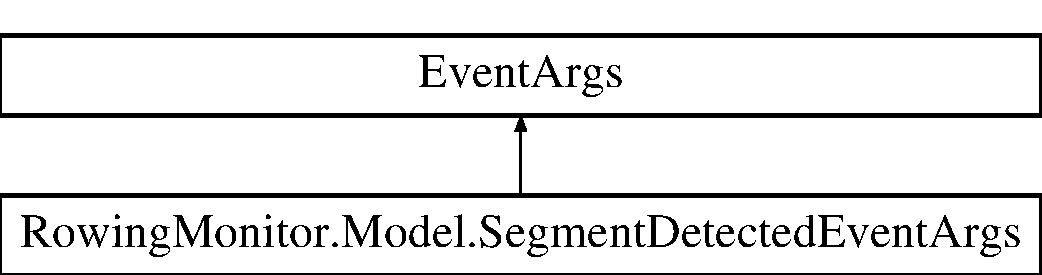
\includegraphics[height=2.000000cm]{class_rowing_monitor_1_1_model_1_1_segment_detected_event_args}
\end{center}
\end{figure}
\subsection*{Public Member Functions}
\begin{DoxyCompactItemize}
\item 
\hyperlink{class_rowing_monitor_1_1_model_1_1_segment_detected_event_args_ae0faa5e59bb3acdbfed39c7f1a44bd4d}{Segment\+Detected\+Event\+Args} (List$<$ \hyperlink{struct_rowing_monitor_1_1_model_1_1_util_1_1_segment_hit}{Segment\+Hit} $>$ hits)
\end{DoxyCompactItemize}
\subsection*{Properties}
\begin{DoxyCompactItemize}
\item 
List$<$ \hyperlink{struct_rowing_monitor_1_1_model_1_1_util_1_1_segment_hit}{Segment\+Hit} $>$ \hyperlink{class_rowing_monitor_1_1_model_1_1_segment_detected_event_args_aa2a7633ef1c061df79fb2932261e0359}{Hits}\hspace{0.3cm}{\ttfamily  \mbox{[}get\mbox{]}}
\end{DoxyCompactItemize}


\subsection{Detailed Description}
Represents the arguments for a detected segment event. 



\subsection{Constructor \& Destructor Documentation}
\mbox{\Hypertarget{class_rowing_monitor_1_1_model_1_1_segment_detected_event_args_ae0faa5e59bb3acdbfed39c7f1a44bd4d}\label{class_rowing_monitor_1_1_model_1_1_segment_detected_event_args_ae0faa5e59bb3acdbfed39c7f1a44bd4d}} 
\index{Rowing\+Monitor\+::\+Model\+::\+Segment\+Detected\+Event\+Args@{Rowing\+Monitor\+::\+Model\+::\+Segment\+Detected\+Event\+Args}!Segment\+Detected\+Event\+Args@{Segment\+Detected\+Event\+Args}}
\index{Segment\+Detected\+Event\+Args@{Segment\+Detected\+Event\+Args}!Rowing\+Monitor\+::\+Model\+::\+Segment\+Detected\+Event\+Args@{Rowing\+Monitor\+::\+Model\+::\+Segment\+Detected\+Event\+Args}}
\subsubsection{\texorpdfstring{Segment\+Detected\+Event\+Args()}{SegmentDetectedEventArgs()}}
{\footnotesize\ttfamily Rowing\+Monitor.\+Model.\+Segment\+Detected\+Event\+Args.\+Segment\+Detected\+Event\+Args (\begin{DoxyParamCaption}\item[{List$<$ \hyperlink{struct_rowing_monitor_1_1_model_1_1_util_1_1_segment_hit}{Segment\+Hit} $>$}]{hits }\end{DoxyParamCaption})}



\subsection{Property Documentation}
\mbox{\Hypertarget{class_rowing_monitor_1_1_model_1_1_segment_detected_event_args_aa2a7633ef1c061df79fb2932261e0359}\label{class_rowing_monitor_1_1_model_1_1_segment_detected_event_args_aa2a7633ef1c061df79fb2932261e0359}} 
\index{Rowing\+Monitor\+::\+Model\+::\+Segment\+Detected\+Event\+Args@{Rowing\+Monitor\+::\+Model\+::\+Segment\+Detected\+Event\+Args}!Hits@{Hits}}
\index{Hits@{Hits}!Rowing\+Monitor\+::\+Model\+::\+Segment\+Detected\+Event\+Args@{Rowing\+Monitor\+::\+Model\+::\+Segment\+Detected\+Event\+Args}}
\subsubsection{\texorpdfstring{Hits}{Hits}}
{\footnotesize\ttfamily List$<$\hyperlink{struct_rowing_monitor_1_1_model_1_1_util_1_1_segment_hit}{Segment\+Hit}$>$ Rowing\+Monitor.\+Model.\+Segment\+Detected\+Event\+Args.\+Hits\hspace{0.3cm}{\ttfamily [get]}}



The documentation for this class was generated from the following file\+:\begin{DoxyCompactItemize}
\item 
Model/\+Event\+Args/\hyperlink{_segment_detected_event_args_8cs}{Segment\+Detected\+Event\+Args.\+cs}\end{DoxyCompactItemize}

\hypertarget{class_rowing_monitor_1_1_model_1_1_pipeline_1_1_segment_detector}{}\section{Rowing\+Monitor.\+Model.\+Pipeline.\+Segment\+Detector Class Reference}
\label{class_rowing_monitor_1_1_model_1_1_pipeline_1_1_segment_detector}\index{Rowing\+Monitor.\+Model.\+Pipeline.\+Segment\+Detector@{Rowing\+Monitor.\+Model.\+Pipeline.\+Segment\+Detector}}
Inheritance diagram for Rowing\+Monitor.\+Model.\+Pipeline.\+Segment\+Detector\+:\begin{figure}[H]
\begin{center}
\leavevmode
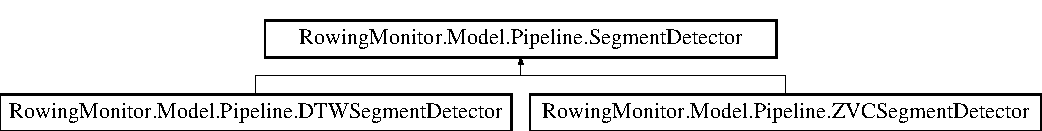
\includegraphics[height=1.755486cm]{class_rowing_monitor_1_1_model_1_1_pipeline_1_1_segment_detector}
\end{center}
\end{figure}
\subsection*{Public Member Functions}
\begin{DoxyCompactItemize}
\item 
delegate void \hyperlink{class_rowing_monitor_1_1_model_1_1_pipeline_1_1_segment_detector_aee5283f7fa49f68c5c4195449442093c}{Segment\+Detected\+Event\+Handler} (Object sender, \hyperlink{class_rowing_monitor_1_1_model_1_1_segment_detected_event_args}{Segment\+Detected\+Event\+Args} e)
\item 
abstract void \hyperlink{class_rowing_monitor_1_1_model_1_1_pipeline_1_1_segment_detector_a24dcb2926660a6218af3052f147d82da}{Update} (\hyperlink{struct_rowing_monitor_1_1_model_1_1_util_1_1_joint_data}{Joint\+Data} joint\+Data, Joint\+Type joint\+Type, String axis)
\item 
abstract List$<$ \hyperlink{struct_rowing_monitor_1_1_model_1_1_util_1_1_segment_hit}{Segment\+Hit} $>$ \hyperlink{class_rowing_monitor_1_1_model_1_1_pipeline_1_1_segment_detector_a28a3c23d7d350c0e37e9a58ff9a4e16b}{Detect} (\hyperlink{struct_rowing_monitor_1_1_model_1_1_util_1_1_joint_data}{Joint\+Data} joint\+Data, Joint\+Type joint\+Type, String axis)
\end{DoxyCompactItemize}
\subsection*{Protected Member Functions}
\begin{DoxyCompactItemize}
\item 
float \hyperlink{class_rowing_monitor_1_1_model_1_1_pipeline_1_1_segment_detector_a1f8ffebdfca18aa67a213ca817981161}{Get\+Joint\+Data\+Value} (\hyperlink{struct_rowing_monitor_1_1_model_1_1_util_1_1_joint_data}{Joint\+Data} joint\+Data, Joint\+Type joint\+Type, String axis)
\item 
virtual void \hyperlink{class_rowing_monitor_1_1_model_1_1_pipeline_1_1_segment_detector_a30d5b8752257a3992db11770506f6a8a}{On\+Segment\+Detected} (\hyperlink{class_rowing_monitor_1_1_model_1_1_segment_detected_event_args}{Segment\+Detected\+Event\+Args} e)
\end{DoxyCompactItemize}
\subsection*{Protected Attributes}
\begin{DoxyCompactItemize}
\item 
List$<$ \hyperlink{struct_rowing_monitor_1_1_model_1_1_util_1_1_segment_hit}{Segment\+Hit} $>$ \hyperlink{class_rowing_monitor_1_1_model_1_1_pipeline_1_1_segment_detector_a567492ea6e393bed7c946359cdf7c866}{hits} = new List$<$\hyperlink{struct_rowing_monitor_1_1_model_1_1_util_1_1_segment_hit}{Segment\+Hit}$>$()
\end{DoxyCompactItemize}
\subsection*{Properties}
\begin{DoxyCompactItemize}
\item 
Broadcast\+Block$<$ List$<$ \hyperlink{struct_rowing_monitor_1_1_model_1_1_util_1_1_segment_hit}{Segment\+Hit} $>$ $>$ \hyperlink{class_rowing_monitor_1_1_model_1_1_pipeline_1_1_segment_detector_a2f9933aa3e7251629d0b1676b73a336a}{Output}\hspace{0.3cm}{\ttfamily  \mbox{[}get, set\mbox{]}}
\item 
Joint\+Type \hyperlink{class_rowing_monitor_1_1_model_1_1_pipeline_1_1_segment_detector_a0bc85068e6ac401713535e38c0f1e18d}{Detection\+Joint\+Type}\hspace{0.3cm}{\ttfamily  \mbox{[}get, set\mbox{]}}
\item 
string \hyperlink{class_rowing_monitor_1_1_model_1_1_pipeline_1_1_segment_detector_ae8b2b75b70356efbe159de7427eb31fd}{Detection\+Axis}\hspace{0.3cm}{\ttfamily  \mbox{[}get, set\mbox{]}}
\item 
Action\+Block$<$ \hyperlink{struct_rowing_monitor_1_1_model_1_1_util_1_1_joint_data}{Joint\+Data} $>$ \hyperlink{class_rowing_monitor_1_1_model_1_1_pipeline_1_1_segment_detector_a1dff97a3144d7642595a8ce1fd4831a4}{Input}\hspace{0.3cm}{\ttfamily  \mbox{[}get, set\mbox{]}}
\end{DoxyCompactItemize}
\subsection*{Events}
\begin{DoxyCompactItemize}
\item 
\hyperlink{class_rowing_monitor_1_1_model_1_1_pipeline_1_1_segment_detector_aee5283f7fa49f68c5c4195449442093c}{Segment\+Detected\+Event\+Handler} \hyperlink{class_rowing_monitor_1_1_model_1_1_pipeline_1_1_segment_detector_aecedec106356c5d32e43e9c9471f12a3}{Segment\+Detected}
\end{DoxyCompactItemize}


\subsection{Member Function Documentation}
\mbox{\Hypertarget{class_rowing_monitor_1_1_model_1_1_pipeline_1_1_segment_detector_a28a3c23d7d350c0e37e9a58ff9a4e16b}\label{class_rowing_monitor_1_1_model_1_1_pipeline_1_1_segment_detector_a28a3c23d7d350c0e37e9a58ff9a4e16b}} 
\index{Rowing\+Monitor\+::\+Model\+::\+Pipeline\+::\+Segment\+Detector@{Rowing\+Monitor\+::\+Model\+::\+Pipeline\+::\+Segment\+Detector}!Detect@{Detect}}
\index{Detect@{Detect}!Rowing\+Monitor\+::\+Model\+::\+Pipeline\+::\+Segment\+Detector@{Rowing\+Monitor\+::\+Model\+::\+Pipeline\+::\+Segment\+Detector}}
\subsubsection{\texorpdfstring{Detect()}{Detect()}}
{\footnotesize\ttfamily abstract List$<$\hyperlink{struct_rowing_monitor_1_1_model_1_1_util_1_1_segment_hit}{Segment\+Hit}$>$ Rowing\+Monitor.\+Model.\+Pipeline.\+Segment\+Detector.\+Detect (\begin{DoxyParamCaption}\item[{\hyperlink{struct_rowing_monitor_1_1_model_1_1_util_1_1_joint_data}{Joint\+Data}}]{joint\+Data,  }\item[{Joint\+Type}]{joint\+Type,  }\item[{String}]{axis }\end{DoxyParamCaption})\hspace{0.3cm}{\ttfamily [pure virtual]}}

\mbox{\Hypertarget{class_rowing_monitor_1_1_model_1_1_pipeline_1_1_segment_detector_a1f8ffebdfca18aa67a213ca817981161}\label{class_rowing_monitor_1_1_model_1_1_pipeline_1_1_segment_detector_a1f8ffebdfca18aa67a213ca817981161}} 
\index{Rowing\+Monitor\+::\+Model\+::\+Pipeline\+::\+Segment\+Detector@{Rowing\+Monitor\+::\+Model\+::\+Pipeline\+::\+Segment\+Detector}!Get\+Joint\+Data\+Value@{Get\+Joint\+Data\+Value}}
\index{Get\+Joint\+Data\+Value@{Get\+Joint\+Data\+Value}!Rowing\+Monitor\+::\+Model\+::\+Pipeline\+::\+Segment\+Detector@{Rowing\+Monitor\+::\+Model\+::\+Pipeline\+::\+Segment\+Detector}}
\subsubsection{\texorpdfstring{Get\+Joint\+Data\+Value()}{GetJointDataValue()}}
{\footnotesize\ttfamily float Rowing\+Monitor.\+Model.\+Pipeline.\+Segment\+Detector.\+Get\+Joint\+Data\+Value (\begin{DoxyParamCaption}\item[{\hyperlink{struct_rowing_monitor_1_1_model_1_1_util_1_1_joint_data}{Joint\+Data}}]{joint\+Data,  }\item[{Joint\+Type}]{joint\+Type,  }\item[{String}]{axis }\end{DoxyParamCaption})\hspace{0.3cm}{\ttfamily [protected]}}

\mbox{\Hypertarget{class_rowing_monitor_1_1_model_1_1_pipeline_1_1_segment_detector_a30d5b8752257a3992db11770506f6a8a}\label{class_rowing_monitor_1_1_model_1_1_pipeline_1_1_segment_detector_a30d5b8752257a3992db11770506f6a8a}} 
\index{Rowing\+Monitor\+::\+Model\+::\+Pipeline\+::\+Segment\+Detector@{Rowing\+Monitor\+::\+Model\+::\+Pipeline\+::\+Segment\+Detector}!On\+Segment\+Detected@{On\+Segment\+Detected}}
\index{On\+Segment\+Detected@{On\+Segment\+Detected}!Rowing\+Monitor\+::\+Model\+::\+Pipeline\+::\+Segment\+Detector@{Rowing\+Monitor\+::\+Model\+::\+Pipeline\+::\+Segment\+Detector}}
\subsubsection{\texorpdfstring{On\+Segment\+Detected()}{OnSegmentDetected()}}
{\footnotesize\ttfamily virtual void Rowing\+Monitor.\+Model.\+Pipeline.\+Segment\+Detector.\+On\+Segment\+Detected (\begin{DoxyParamCaption}\item[{\hyperlink{class_rowing_monitor_1_1_model_1_1_segment_detected_event_args}{Segment\+Detected\+Event\+Args}}]{e }\end{DoxyParamCaption})\hspace{0.3cm}{\ttfamily [protected]}, {\ttfamily [virtual]}}



Reimplemented in \hyperlink{class_rowing_monitor_1_1_model_1_1_pipeline_1_1_z_v_c_segment_detector_a5eab838eda9f217722dfa05bc9d5095b}{Rowing\+Monitor.\+Model.\+Pipeline.\+Z\+V\+C\+Segment\+Detector}, and \hyperlink{class_rowing_monitor_1_1_model_1_1_pipeline_1_1_d_t_w_segment_detector_a6d2644f751e290cef82649c42becdd92}{Rowing\+Monitor.\+Model.\+Pipeline.\+D\+T\+W\+Segment\+Detector}.

\mbox{\Hypertarget{class_rowing_monitor_1_1_model_1_1_pipeline_1_1_segment_detector_aee5283f7fa49f68c5c4195449442093c}\label{class_rowing_monitor_1_1_model_1_1_pipeline_1_1_segment_detector_aee5283f7fa49f68c5c4195449442093c}} 
\index{Rowing\+Monitor\+::\+Model\+::\+Pipeline\+::\+Segment\+Detector@{Rowing\+Monitor\+::\+Model\+::\+Pipeline\+::\+Segment\+Detector}!Segment\+Detected\+Event\+Handler@{Segment\+Detected\+Event\+Handler}}
\index{Segment\+Detected\+Event\+Handler@{Segment\+Detected\+Event\+Handler}!Rowing\+Monitor\+::\+Model\+::\+Pipeline\+::\+Segment\+Detector@{Rowing\+Monitor\+::\+Model\+::\+Pipeline\+::\+Segment\+Detector}}
\subsubsection{\texorpdfstring{Segment\+Detected\+Event\+Handler()}{SegmentDetectedEventHandler()}}
{\footnotesize\ttfamily delegate void Rowing\+Monitor.\+Model.\+Pipeline.\+Segment\+Detector.\+Segment\+Detected\+Event\+Handler (\begin{DoxyParamCaption}\item[{Object}]{sender,  }\item[{\hyperlink{class_rowing_monitor_1_1_model_1_1_segment_detected_event_args}{Segment\+Detected\+Event\+Args}}]{e }\end{DoxyParamCaption})}

\mbox{\Hypertarget{class_rowing_monitor_1_1_model_1_1_pipeline_1_1_segment_detector_a24dcb2926660a6218af3052f147d82da}\label{class_rowing_monitor_1_1_model_1_1_pipeline_1_1_segment_detector_a24dcb2926660a6218af3052f147d82da}} 
\index{Rowing\+Monitor\+::\+Model\+::\+Pipeline\+::\+Segment\+Detector@{Rowing\+Monitor\+::\+Model\+::\+Pipeline\+::\+Segment\+Detector}!Update@{Update}}
\index{Update@{Update}!Rowing\+Monitor\+::\+Model\+::\+Pipeline\+::\+Segment\+Detector@{Rowing\+Monitor\+::\+Model\+::\+Pipeline\+::\+Segment\+Detector}}
\subsubsection{\texorpdfstring{Update()}{Update()}}
{\footnotesize\ttfamily abstract void Rowing\+Monitor.\+Model.\+Pipeline.\+Segment\+Detector.\+Update (\begin{DoxyParamCaption}\item[{\hyperlink{struct_rowing_monitor_1_1_model_1_1_util_1_1_joint_data}{Joint\+Data}}]{joint\+Data,  }\item[{Joint\+Type}]{joint\+Type,  }\item[{String}]{axis }\end{DoxyParamCaption})\hspace{0.3cm}{\ttfamily [pure virtual]}}



Implemented in \hyperlink{class_rowing_monitor_1_1_model_1_1_pipeline_1_1_z_v_c_segment_detector_a81c28e4ede1561c2fe1eca29f63f0767}{Rowing\+Monitor.\+Model.\+Pipeline.\+Z\+V\+C\+Segment\+Detector}.



\subsection{Member Data Documentation}
\mbox{\Hypertarget{class_rowing_monitor_1_1_model_1_1_pipeline_1_1_segment_detector_a567492ea6e393bed7c946359cdf7c866}\label{class_rowing_monitor_1_1_model_1_1_pipeline_1_1_segment_detector_a567492ea6e393bed7c946359cdf7c866}} 
\index{Rowing\+Monitor\+::\+Model\+::\+Pipeline\+::\+Segment\+Detector@{Rowing\+Monitor\+::\+Model\+::\+Pipeline\+::\+Segment\+Detector}!hits@{hits}}
\index{hits@{hits}!Rowing\+Monitor\+::\+Model\+::\+Pipeline\+::\+Segment\+Detector@{Rowing\+Monitor\+::\+Model\+::\+Pipeline\+::\+Segment\+Detector}}
\subsubsection{\texorpdfstring{hits}{hits}}
{\footnotesize\ttfamily List$<$\hyperlink{struct_rowing_monitor_1_1_model_1_1_util_1_1_segment_hit}{Segment\+Hit}$>$ Rowing\+Monitor.\+Model.\+Pipeline.\+Segment\+Detector.\+hits = new List$<$\hyperlink{struct_rowing_monitor_1_1_model_1_1_util_1_1_segment_hit}{Segment\+Hit}$>$()\hspace{0.3cm}{\ttfamily [protected]}}



\subsection{Property Documentation}
\mbox{\Hypertarget{class_rowing_monitor_1_1_model_1_1_pipeline_1_1_segment_detector_ae8b2b75b70356efbe159de7427eb31fd}\label{class_rowing_monitor_1_1_model_1_1_pipeline_1_1_segment_detector_ae8b2b75b70356efbe159de7427eb31fd}} 
\index{Rowing\+Monitor\+::\+Model\+::\+Pipeline\+::\+Segment\+Detector@{Rowing\+Monitor\+::\+Model\+::\+Pipeline\+::\+Segment\+Detector}!Detection\+Axis@{Detection\+Axis}}
\index{Detection\+Axis@{Detection\+Axis}!Rowing\+Monitor\+::\+Model\+::\+Pipeline\+::\+Segment\+Detector@{Rowing\+Monitor\+::\+Model\+::\+Pipeline\+::\+Segment\+Detector}}
\subsubsection{\texorpdfstring{Detection\+Axis}{DetectionAxis}}
{\footnotesize\ttfamily string Rowing\+Monitor.\+Model.\+Pipeline.\+Segment\+Detector.\+Detection\+Axis\hspace{0.3cm}{\ttfamily [get]}, {\ttfamily [set]}}

\mbox{\Hypertarget{class_rowing_monitor_1_1_model_1_1_pipeline_1_1_segment_detector_a0bc85068e6ac401713535e38c0f1e18d}\label{class_rowing_monitor_1_1_model_1_1_pipeline_1_1_segment_detector_a0bc85068e6ac401713535e38c0f1e18d}} 
\index{Rowing\+Monitor\+::\+Model\+::\+Pipeline\+::\+Segment\+Detector@{Rowing\+Monitor\+::\+Model\+::\+Pipeline\+::\+Segment\+Detector}!Detection\+Joint\+Type@{Detection\+Joint\+Type}}
\index{Detection\+Joint\+Type@{Detection\+Joint\+Type}!Rowing\+Monitor\+::\+Model\+::\+Pipeline\+::\+Segment\+Detector@{Rowing\+Monitor\+::\+Model\+::\+Pipeline\+::\+Segment\+Detector}}
\subsubsection{\texorpdfstring{Detection\+Joint\+Type}{DetectionJointType}}
{\footnotesize\ttfamily Joint\+Type Rowing\+Monitor.\+Model.\+Pipeline.\+Segment\+Detector.\+Detection\+Joint\+Type\hspace{0.3cm}{\ttfamily [get]}, {\ttfamily [set]}}

\mbox{\Hypertarget{class_rowing_monitor_1_1_model_1_1_pipeline_1_1_segment_detector_a1dff97a3144d7642595a8ce1fd4831a4}\label{class_rowing_monitor_1_1_model_1_1_pipeline_1_1_segment_detector_a1dff97a3144d7642595a8ce1fd4831a4}} 
\index{Rowing\+Monitor\+::\+Model\+::\+Pipeline\+::\+Segment\+Detector@{Rowing\+Monitor\+::\+Model\+::\+Pipeline\+::\+Segment\+Detector}!Input@{Input}}
\index{Input@{Input}!Rowing\+Monitor\+::\+Model\+::\+Pipeline\+::\+Segment\+Detector@{Rowing\+Monitor\+::\+Model\+::\+Pipeline\+::\+Segment\+Detector}}
\subsubsection{\texorpdfstring{Input}{Input}}
{\footnotesize\ttfamily Action\+Block$<$\hyperlink{struct_rowing_monitor_1_1_model_1_1_util_1_1_joint_data}{Joint\+Data}$>$ Rowing\+Monitor.\+Model.\+Pipeline.\+Segment\+Detector.\+Input\hspace{0.3cm}{\ttfamily [get]}, {\ttfamily [set]}}

\mbox{\Hypertarget{class_rowing_monitor_1_1_model_1_1_pipeline_1_1_segment_detector_a2f9933aa3e7251629d0b1676b73a336a}\label{class_rowing_monitor_1_1_model_1_1_pipeline_1_1_segment_detector_a2f9933aa3e7251629d0b1676b73a336a}} 
\index{Rowing\+Monitor\+::\+Model\+::\+Pipeline\+::\+Segment\+Detector@{Rowing\+Monitor\+::\+Model\+::\+Pipeline\+::\+Segment\+Detector}!Output@{Output}}
\index{Output@{Output}!Rowing\+Monitor\+::\+Model\+::\+Pipeline\+::\+Segment\+Detector@{Rowing\+Monitor\+::\+Model\+::\+Pipeline\+::\+Segment\+Detector}}
\subsubsection{\texorpdfstring{Output}{Output}}
{\footnotesize\ttfamily Broadcast\+Block$<$List$<$\hyperlink{struct_rowing_monitor_1_1_model_1_1_util_1_1_segment_hit}{Segment\+Hit}$>$ $>$ Rowing\+Monitor.\+Model.\+Pipeline.\+Segment\+Detector.\+Output\hspace{0.3cm}{\ttfamily [get]}, {\ttfamily [set]}}



\subsection{Event Documentation}
\mbox{\Hypertarget{class_rowing_monitor_1_1_model_1_1_pipeline_1_1_segment_detector_aecedec106356c5d32e43e9c9471f12a3}\label{class_rowing_monitor_1_1_model_1_1_pipeline_1_1_segment_detector_aecedec106356c5d32e43e9c9471f12a3}} 
\index{Rowing\+Monitor\+::\+Model\+::\+Pipeline\+::\+Segment\+Detector@{Rowing\+Monitor\+::\+Model\+::\+Pipeline\+::\+Segment\+Detector}!Segment\+Detected@{Segment\+Detected}}
\index{Segment\+Detected@{Segment\+Detected}!Rowing\+Monitor\+::\+Model\+::\+Pipeline\+::\+Segment\+Detector@{Rowing\+Monitor\+::\+Model\+::\+Pipeline\+::\+Segment\+Detector}}
\subsubsection{\texorpdfstring{Segment\+Detected}{SegmentDetected}}
{\footnotesize\ttfamily \hyperlink{class_rowing_monitor_1_1_model_1_1_pipeline_1_1_segment_detector_aee5283f7fa49f68c5c4195449442093c}{Segment\+Detected\+Event\+Handler} Rowing\+Monitor.\+Model.\+Pipeline.\+Segment\+Detector.\+Segment\+Detected}



The documentation for this class was generated from the following file\+:\begin{DoxyCompactItemize}
\item 
Model/\+Pipeline/\hyperlink{_segment_detector_8cs}{Segment\+Detector.\+cs}\end{DoxyCompactItemize}

\hypertarget{struct_rowing_monitor_1_1_model_1_1_util_1_1_segment_hit}{}\section{Rowing\+Monitor.\+Model.\+Util.\+Segment\+Hit Struct Reference}
\label{struct_rowing_monitor_1_1_model_1_1_util_1_1_segment_hit}\index{Rowing\+Monitor.\+Model.\+Util.\+Segment\+Hit@{Rowing\+Monitor.\+Model.\+Util.\+Segment\+Hit}}
\subsection*{Properties}
\begin{DoxyCompactItemize}
\item 
long \hyperlink{struct_rowing_monitor_1_1_model_1_1_util_1_1_segment_hit_aaf855f224da3b43af2ea5f7896914efb}{Index}\hspace{0.3cm}{\ttfamily  \mbox{[}get, set\mbox{]}}
\begin{DoxyCompactList}\small\item\em Index of the joint data that this hit belongs to. \end{DoxyCompactList}\item 
long \hyperlink{struct_rowing_monitor_1_1_model_1_1_util_1_1_segment_hit_ad943df68e8adfeaa2b76701701cef0df}{Detection\+Index}\hspace{0.3cm}{\ttfamily  \mbox{[}get, set\mbox{]}}
\begin{DoxyCompactList}\small\item\em Index of the joint data where this hit was detected. \end{DoxyCompactList}\item 
double \hyperlink{struct_rowing_monitor_1_1_model_1_1_util_1_1_segment_hit_ab40df6a59087cfd176f989111279a5e2}{Abs\+Timestamp}\hspace{0.3cm}{\ttfamily  \mbox{[}get, set\mbox{]}}
\begin{DoxyCompactList}\small\item\em Absolute timestamp of the joint data that this hit belongs to. \end{DoxyCompactList}\item 
double \hyperlink{struct_rowing_monitor_1_1_model_1_1_util_1_1_segment_hit_ab9778fc572f014c1d75de5898f8c83d2}{Detection\+Abs\+Timestamp}\hspace{0.3cm}{\ttfamily  \mbox{[}get, set\mbox{]}}
\begin{DoxyCompactList}\small\item\em Absolute timestamp of the joint data where this hit was detected. \end{DoxyCompactList}\item 
\hyperlink{namespace_rowing_monitor_1_1_model_1_1_util_a7135d50f11f02e6f0cb9680dc68dba56}{Hit\+Type} \hyperlink{struct_rowing_monitor_1_1_model_1_1_util_1_1_segment_hit_ab2a359ba79fbc8456596219484f2a159}{Hit\+Type}\hspace{0.3cm}{\ttfamily  \mbox{[}get, set\mbox{]}}
\begin{DoxyCompactList}\small\item\em Type of this hit in the context of a segment. \end{DoxyCompactList}\end{DoxyCompactItemize}


\subsection{Property Documentation}
\mbox{\Hypertarget{struct_rowing_monitor_1_1_model_1_1_util_1_1_segment_hit_ab40df6a59087cfd176f989111279a5e2}\label{struct_rowing_monitor_1_1_model_1_1_util_1_1_segment_hit_ab40df6a59087cfd176f989111279a5e2}} 
\index{Rowing\+Monitor\+::\+Model\+::\+Util\+::\+Segment\+Hit@{Rowing\+Monitor\+::\+Model\+::\+Util\+::\+Segment\+Hit}!Abs\+Timestamp@{Abs\+Timestamp}}
\index{Abs\+Timestamp@{Abs\+Timestamp}!Rowing\+Monitor\+::\+Model\+::\+Util\+::\+Segment\+Hit@{Rowing\+Monitor\+::\+Model\+::\+Util\+::\+Segment\+Hit}}
\subsubsection{\texorpdfstring{Abs\+Timestamp}{AbsTimestamp}}
{\footnotesize\ttfamily double Rowing\+Monitor.\+Model.\+Util.\+Segment\+Hit.\+Abs\+Timestamp\hspace{0.3cm}{\ttfamily [get]}, {\ttfamily [set]}}



Absolute timestamp of the joint data that this hit belongs to. 

\mbox{\Hypertarget{struct_rowing_monitor_1_1_model_1_1_util_1_1_segment_hit_ab9778fc572f014c1d75de5898f8c83d2}\label{struct_rowing_monitor_1_1_model_1_1_util_1_1_segment_hit_ab9778fc572f014c1d75de5898f8c83d2}} 
\index{Rowing\+Monitor\+::\+Model\+::\+Util\+::\+Segment\+Hit@{Rowing\+Monitor\+::\+Model\+::\+Util\+::\+Segment\+Hit}!Detection\+Abs\+Timestamp@{Detection\+Abs\+Timestamp}}
\index{Detection\+Abs\+Timestamp@{Detection\+Abs\+Timestamp}!Rowing\+Monitor\+::\+Model\+::\+Util\+::\+Segment\+Hit@{Rowing\+Monitor\+::\+Model\+::\+Util\+::\+Segment\+Hit}}
\subsubsection{\texorpdfstring{Detection\+Abs\+Timestamp}{DetectionAbsTimestamp}}
{\footnotesize\ttfamily double Rowing\+Monitor.\+Model.\+Util.\+Segment\+Hit.\+Detection\+Abs\+Timestamp\hspace{0.3cm}{\ttfamily [get]}, {\ttfamily [set]}}



Absolute timestamp of the joint data where this hit was detected. 

\mbox{\Hypertarget{struct_rowing_monitor_1_1_model_1_1_util_1_1_segment_hit_ad943df68e8adfeaa2b76701701cef0df}\label{struct_rowing_monitor_1_1_model_1_1_util_1_1_segment_hit_ad943df68e8adfeaa2b76701701cef0df}} 
\index{Rowing\+Monitor\+::\+Model\+::\+Util\+::\+Segment\+Hit@{Rowing\+Monitor\+::\+Model\+::\+Util\+::\+Segment\+Hit}!Detection\+Index@{Detection\+Index}}
\index{Detection\+Index@{Detection\+Index}!Rowing\+Monitor\+::\+Model\+::\+Util\+::\+Segment\+Hit@{Rowing\+Monitor\+::\+Model\+::\+Util\+::\+Segment\+Hit}}
\subsubsection{\texorpdfstring{Detection\+Index}{DetectionIndex}}
{\footnotesize\ttfamily long Rowing\+Monitor.\+Model.\+Util.\+Segment\+Hit.\+Detection\+Index\hspace{0.3cm}{\ttfamily [get]}, {\ttfamily [set]}}



Index of the joint data where this hit was detected. 

\mbox{\Hypertarget{struct_rowing_monitor_1_1_model_1_1_util_1_1_segment_hit_ab2a359ba79fbc8456596219484f2a159}\label{struct_rowing_monitor_1_1_model_1_1_util_1_1_segment_hit_ab2a359ba79fbc8456596219484f2a159}} 
\index{Rowing\+Monitor\+::\+Model\+::\+Util\+::\+Segment\+Hit@{Rowing\+Monitor\+::\+Model\+::\+Util\+::\+Segment\+Hit}!Hit\+Type@{Hit\+Type}}
\index{Hit\+Type@{Hit\+Type}!Rowing\+Monitor\+::\+Model\+::\+Util\+::\+Segment\+Hit@{Rowing\+Monitor\+::\+Model\+::\+Util\+::\+Segment\+Hit}}
\subsubsection{\texorpdfstring{Hit\+Type}{HitType}}
{\footnotesize\ttfamily \hyperlink{namespace_rowing_monitor_1_1_model_1_1_util_a7135d50f11f02e6f0cb9680dc68dba56}{Hit\+Type} Rowing\+Monitor.\+Model.\+Util.\+Segment\+Hit.\+Hit\+Type\hspace{0.3cm}{\ttfamily [get]}, {\ttfamily [set]}}



Type of this hit in the context of a segment. 

\mbox{\Hypertarget{struct_rowing_monitor_1_1_model_1_1_util_1_1_segment_hit_aaf855f224da3b43af2ea5f7896914efb}\label{struct_rowing_monitor_1_1_model_1_1_util_1_1_segment_hit_aaf855f224da3b43af2ea5f7896914efb}} 
\index{Rowing\+Monitor\+::\+Model\+::\+Util\+::\+Segment\+Hit@{Rowing\+Monitor\+::\+Model\+::\+Util\+::\+Segment\+Hit}!Index@{Index}}
\index{Index@{Index}!Rowing\+Monitor\+::\+Model\+::\+Util\+::\+Segment\+Hit@{Rowing\+Monitor\+::\+Model\+::\+Util\+::\+Segment\+Hit}}
\subsubsection{\texorpdfstring{Index}{Index}}
{\footnotesize\ttfamily long Rowing\+Monitor.\+Model.\+Util.\+Segment\+Hit.\+Index\hspace{0.3cm}{\ttfamily [get]}, {\ttfamily [set]}}



Index of the joint data that this hit belongs to. 



The documentation for this struct was generated from the following file\+:\begin{DoxyCompactItemize}
\item 
Model/\+Util/\hyperlink{_kinect_data_handler_8cs}{Kinect\+Data\+Handler.\+cs}\end{DoxyCompactItemize}

\hypertarget{class_rowing_monitor_1_1_model_1_1_shifted_frame_arrived_event_args}{}\section{Rowing\+Monitor.\+Model.\+Shifted\+Frame\+Arrived\+Event\+Args Class Reference}
\label{class_rowing_monitor_1_1_model_1_1_shifted_frame_arrived_event_args}\index{Rowing\+Monitor.\+Model.\+Shifted\+Frame\+Arrived\+Event\+Args@{Rowing\+Monitor.\+Model.\+Shifted\+Frame\+Arrived\+Event\+Args}}


Represents the arguments for a shifted frame arrived event.  


Inheritance diagram for Rowing\+Monitor.\+Model.\+Shifted\+Frame\+Arrived\+Event\+Args\+:\begin{figure}[H]
\begin{center}
\leavevmode
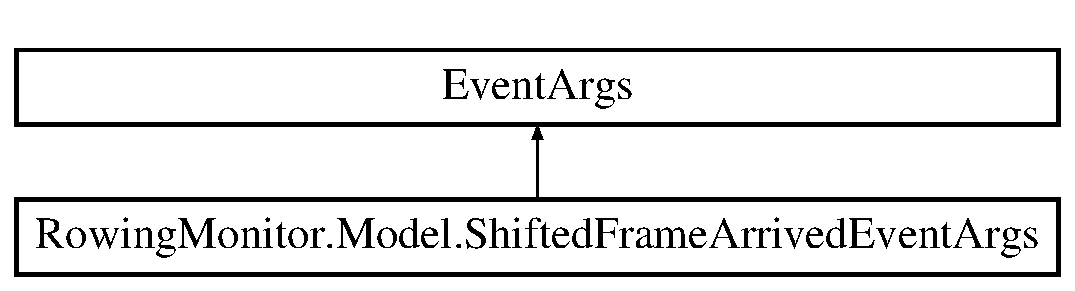
\includegraphics[height=2.000000cm]{class_rowing_monitor_1_1_model_1_1_shifted_frame_arrived_event_args}
\end{center}
\end{figure}
\subsection*{Public Member Functions}
\begin{DoxyCompactItemize}
\item 
\hyperlink{class_rowing_monitor_1_1_model_1_1_shifted_frame_arrived_event_args_a7ea2f2cc785f346a8fc51e770352ef2c}{Shifted\+Frame\+Arrived\+Event\+Args} (\hyperlink{struct_rowing_monitor_1_1_model_1_1_util_1_1_joint_data}{Joint\+Data} shifted\+Joint\+Data)
\end{DoxyCompactItemize}
\subsection*{Properties}
\begin{DoxyCompactItemize}
\item 
\hyperlink{struct_rowing_monitor_1_1_model_1_1_util_1_1_joint_data}{Joint\+Data} \hyperlink{class_rowing_monitor_1_1_model_1_1_shifted_frame_arrived_event_args_a668747182e00705fcaef8d16320ce730}{Shifted\+Joint\+Data}\hspace{0.3cm}{\ttfamily  \mbox{[}get\mbox{]}}
\end{DoxyCompactItemize}


\subsection{Detailed Description}
Represents the arguments for a shifted frame arrived event. 



\subsection{Constructor \& Destructor Documentation}
\mbox{\Hypertarget{class_rowing_monitor_1_1_model_1_1_shifted_frame_arrived_event_args_a7ea2f2cc785f346a8fc51e770352ef2c}\label{class_rowing_monitor_1_1_model_1_1_shifted_frame_arrived_event_args_a7ea2f2cc785f346a8fc51e770352ef2c}} 
\index{Rowing\+Monitor\+::\+Model\+::\+Shifted\+Frame\+Arrived\+Event\+Args@{Rowing\+Monitor\+::\+Model\+::\+Shifted\+Frame\+Arrived\+Event\+Args}!Shifted\+Frame\+Arrived\+Event\+Args@{Shifted\+Frame\+Arrived\+Event\+Args}}
\index{Shifted\+Frame\+Arrived\+Event\+Args@{Shifted\+Frame\+Arrived\+Event\+Args}!Rowing\+Monitor\+::\+Model\+::\+Shifted\+Frame\+Arrived\+Event\+Args@{Rowing\+Monitor\+::\+Model\+::\+Shifted\+Frame\+Arrived\+Event\+Args}}
\subsubsection{\texorpdfstring{Shifted\+Frame\+Arrived\+Event\+Args()}{ShiftedFrameArrivedEventArgs()}}
{\footnotesize\ttfamily Rowing\+Monitor.\+Model.\+Shifted\+Frame\+Arrived\+Event\+Args.\+Shifted\+Frame\+Arrived\+Event\+Args (\begin{DoxyParamCaption}\item[{\hyperlink{struct_rowing_monitor_1_1_model_1_1_util_1_1_joint_data}{Joint\+Data}}]{shifted\+Joint\+Data }\end{DoxyParamCaption})}



\subsection{Property Documentation}
\mbox{\Hypertarget{class_rowing_monitor_1_1_model_1_1_shifted_frame_arrived_event_args_a668747182e00705fcaef8d16320ce730}\label{class_rowing_monitor_1_1_model_1_1_shifted_frame_arrived_event_args_a668747182e00705fcaef8d16320ce730}} 
\index{Rowing\+Monitor\+::\+Model\+::\+Shifted\+Frame\+Arrived\+Event\+Args@{Rowing\+Monitor\+::\+Model\+::\+Shifted\+Frame\+Arrived\+Event\+Args}!Shifted\+Joint\+Data@{Shifted\+Joint\+Data}}
\index{Shifted\+Joint\+Data@{Shifted\+Joint\+Data}!Rowing\+Monitor\+::\+Model\+::\+Shifted\+Frame\+Arrived\+Event\+Args@{Rowing\+Monitor\+::\+Model\+::\+Shifted\+Frame\+Arrived\+Event\+Args}}
\subsubsection{\texorpdfstring{Shifted\+Joint\+Data}{ShiftedJointData}}
{\footnotesize\ttfamily \hyperlink{struct_rowing_monitor_1_1_model_1_1_util_1_1_joint_data}{Joint\+Data} Rowing\+Monitor.\+Model.\+Shifted\+Frame\+Arrived\+Event\+Args.\+Shifted\+Joint\+Data\hspace{0.3cm}{\ttfamily [get]}}



The documentation for this class was generated from the following file\+:\begin{DoxyCompactItemize}
\item 
Model/\+Event\+Args/\hyperlink{_shifted_frame_arrived_event_args_8cs}{Shifted\+Frame\+Arrived\+Event\+Args.\+cs}\end{DoxyCompactItemize}

\hypertarget{class_rowing_monitor_1_1_model_1_1_shifter}{}\section{Rowing\+Monitor.\+Model.\+Shifter Class Reference}
\label{class_rowing_monitor_1_1_model_1_1_shifter}\index{Rowing\+Monitor.\+Model.\+Shifter@{Rowing\+Monitor.\+Model.\+Shifter}}


Shifts the origin to the middle point between the foot ankle joints. Also rotates all joints until origin and hip joint form a horizontal line.  


\subsection*{Public Member Functions}
\begin{DoxyCompactItemize}
\item 
delegate void \hyperlink{class_rowing_monitor_1_1_model_1_1_shifter_a094227f56757ab924211af7a74d0e205}{Shifted\+Frame\+Arrived\+Event\+Handler} (Object sender, \hyperlink{class_rowing_monitor_1_1_model_1_1_shifted_frame_arrived_event_args}{Shifted\+Frame\+Arrived\+Event\+Args} e)
\item 
void \hyperlink{class_rowing_monitor_1_1_model_1_1_shifter_a645e11ed09c90d94fb64ccbcbd12453f}{Shift\+And\+Rotate} (\hyperlink{struct_rowing_monitor_1_1_model_1_1_util_1_1_joint_data}{Joint\+Data} joint\+Data)
\end{DoxyCompactItemize}
\subsection*{Events}
\begin{DoxyCompactItemize}
\item 
\hyperlink{class_rowing_monitor_1_1_model_1_1_shifter_a094227f56757ab924211af7a74d0e205}{Shifted\+Frame\+Arrived\+Event\+Handler} \hyperlink{class_rowing_monitor_1_1_model_1_1_shifter_af95fddf9149c4aa965a6365180954cf7}{Shifted\+Frame\+Arrived}
\end{DoxyCompactItemize}


\subsection{Detailed Description}
Shifts the origin to the middle point between the foot ankle joints. Also rotates all joints until origin and hip joint form a horizontal line. 



\subsection{Member Function Documentation}
\mbox{\Hypertarget{class_rowing_monitor_1_1_model_1_1_shifter_a645e11ed09c90d94fb64ccbcbd12453f}\label{class_rowing_monitor_1_1_model_1_1_shifter_a645e11ed09c90d94fb64ccbcbd12453f}} 
\index{Rowing\+Monitor\+::\+Model\+::\+Shifter@{Rowing\+Monitor\+::\+Model\+::\+Shifter}!Shift\+And\+Rotate@{Shift\+And\+Rotate}}
\index{Shift\+And\+Rotate@{Shift\+And\+Rotate}!Rowing\+Monitor\+::\+Model\+::\+Shifter@{Rowing\+Monitor\+::\+Model\+::\+Shifter}}
\subsubsection{\texorpdfstring{Shift\+And\+Rotate()}{ShiftAndRotate()}}
{\footnotesize\ttfamily void Rowing\+Monitor.\+Model.\+Shifter.\+Shift\+And\+Rotate (\begin{DoxyParamCaption}\item[{\hyperlink{struct_rowing_monitor_1_1_model_1_1_util_1_1_joint_data}{Joint\+Data}}]{joint\+Data }\end{DoxyParamCaption})}

\mbox{\Hypertarget{class_rowing_monitor_1_1_model_1_1_shifter_a094227f56757ab924211af7a74d0e205}\label{class_rowing_monitor_1_1_model_1_1_shifter_a094227f56757ab924211af7a74d0e205}} 
\index{Rowing\+Monitor\+::\+Model\+::\+Shifter@{Rowing\+Monitor\+::\+Model\+::\+Shifter}!Shifted\+Frame\+Arrived\+Event\+Handler@{Shifted\+Frame\+Arrived\+Event\+Handler}}
\index{Shifted\+Frame\+Arrived\+Event\+Handler@{Shifted\+Frame\+Arrived\+Event\+Handler}!Rowing\+Monitor\+::\+Model\+::\+Shifter@{Rowing\+Monitor\+::\+Model\+::\+Shifter}}
\subsubsection{\texorpdfstring{Shifted\+Frame\+Arrived\+Event\+Handler()}{ShiftedFrameArrivedEventHandler()}}
{\footnotesize\ttfamily delegate void Rowing\+Monitor.\+Model.\+Shifter.\+Shifted\+Frame\+Arrived\+Event\+Handler (\begin{DoxyParamCaption}\item[{Object}]{sender,  }\item[{\hyperlink{class_rowing_monitor_1_1_model_1_1_shifted_frame_arrived_event_args}{Shifted\+Frame\+Arrived\+Event\+Args}}]{e }\end{DoxyParamCaption})}



\subsection{Event Documentation}
\mbox{\Hypertarget{class_rowing_monitor_1_1_model_1_1_shifter_af95fddf9149c4aa965a6365180954cf7}\label{class_rowing_monitor_1_1_model_1_1_shifter_af95fddf9149c4aa965a6365180954cf7}} 
\index{Rowing\+Monitor\+::\+Model\+::\+Shifter@{Rowing\+Monitor\+::\+Model\+::\+Shifter}!Shifted\+Frame\+Arrived@{Shifted\+Frame\+Arrived}}
\index{Shifted\+Frame\+Arrived@{Shifted\+Frame\+Arrived}!Rowing\+Monitor\+::\+Model\+::\+Shifter@{Rowing\+Monitor\+::\+Model\+::\+Shifter}}
\subsubsection{\texorpdfstring{Shifted\+Frame\+Arrived}{ShiftedFrameArrived}}
{\footnotesize\ttfamily \hyperlink{class_rowing_monitor_1_1_model_1_1_shifter_a094227f56757ab924211af7a74d0e205}{Shifted\+Frame\+Arrived\+Event\+Handler} Rowing\+Monitor.\+Model.\+Shifter.\+Shifted\+Frame\+Arrived}



The documentation for this class was generated from the following file\+:\begin{DoxyCompactItemize}
\item 
Model/\+Pipeline/\hyperlink{_shifter_8cs}{Shifter.\+cs}\end{DoxyCompactItemize}

\hypertarget{class_rowing_monitor_1_1_model_1_1_side_view}{}\section{Rowing\+Monitor.\+Model.\+Side\+View Class Reference}
\label{class_rowing_monitor_1_1_model_1_1_side_view}\index{Rowing\+Monitor.\+Model.\+Side\+View@{Rowing\+Monitor.\+Model.\+Side\+View}}
Inheritance diagram for Rowing\+Monitor.\+Model.\+Side\+View\+:\begin{figure}[H]
\begin{center}
\leavevmode
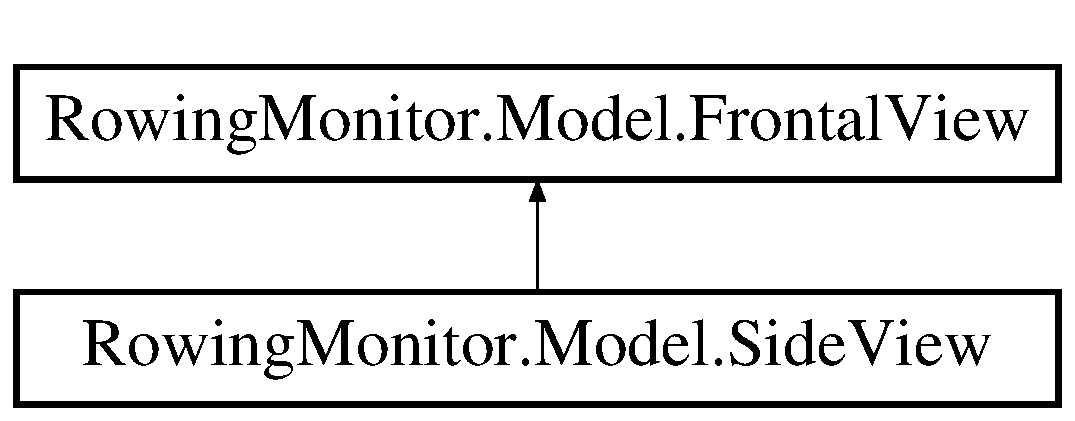
\includegraphics[height=2.000000cm]{class_rowing_monitor_1_1_model_1_1_side_view}
\end{center}
\end{figure}
\subsection*{Public Member Functions}
\begin{DoxyCompactItemize}
\item 
\hyperlink{class_rowing_monitor_1_1_model_1_1_side_view_af647d9e21d8e6add558e57ccc31555f2}{Side\+View} (Coordinate\+Mapper mapper, int width, int height)
\item 
override void \hyperlink{class_rowing_monitor_1_1_model_1_1_side_view_a2cfba6b08a666c71ed25a3cbeaabe138}{Update\+Skeleton} (I\+Read\+Only\+Dictionary$<$ Joint\+Type, Joint $>$ joints)
\begin{DoxyCompactList}\small\item\em Updates the view with new data. \end{DoxyCompactList}\end{DoxyCompactItemize}
\subsection*{Additional Inherited Members}


\subsection{Constructor \& Destructor Documentation}
\mbox{\Hypertarget{class_rowing_monitor_1_1_model_1_1_side_view_af647d9e21d8e6add558e57ccc31555f2}\label{class_rowing_monitor_1_1_model_1_1_side_view_af647d9e21d8e6add558e57ccc31555f2}} 
\index{Rowing\+Monitor\+::\+Model\+::\+Side\+View@{Rowing\+Monitor\+::\+Model\+::\+Side\+View}!Side\+View@{Side\+View}}
\index{Side\+View@{Side\+View}!Rowing\+Monitor\+::\+Model\+::\+Side\+View@{Rowing\+Monitor\+::\+Model\+::\+Side\+View}}
\subsubsection{\texorpdfstring{Side\+View()}{SideView()}}
{\footnotesize\ttfamily Rowing\+Monitor.\+Model.\+Side\+View.\+Side\+View (\begin{DoxyParamCaption}\item[{Coordinate\+Mapper}]{mapper,  }\item[{int}]{width,  }\item[{int}]{height }\end{DoxyParamCaption})}



\subsection{Member Function Documentation}
\mbox{\Hypertarget{class_rowing_monitor_1_1_model_1_1_side_view_a2cfba6b08a666c71ed25a3cbeaabe138}\label{class_rowing_monitor_1_1_model_1_1_side_view_a2cfba6b08a666c71ed25a3cbeaabe138}} 
\index{Rowing\+Monitor\+::\+Model\+::\+Side\+View@{Rowing\+Monitor\+::\+Model\+::\+Side\+View}!Update\+Skeleton@{Update\+Skeleton}}
\index{Update\+Skeleton@{Update\+Skeleton}!Rowing\+Monitor\+::\+Model\+::\+Side\+View@{Rowing\+Monitor\+::\+Model\+::\+Side\+View}}
\subsubsection{\texorpdfstring{Update\+Skeleton()}{UpdateSkeleton()}}
{\footnotesize\ttfamily override void Rowing\+Monitor.\+Model.\+Side\+View.\+Update\+Skeleton (\begin{DoxyParamCaption}\item[{I\+Read\+Only\+Dictionary$<$ Joint\+Type, Joint $>$}]{joints }\end{DoxyParamCaption})\hspace{0.3cm}{\ttfamily [virtual]}}



Updates the view with new data. 



Reimplemented from \hyperlink{class_rowing_monitor_1_1_model_1_1_frontal_view_a3dddfa75ba346fdcf99dbd763e9ea1ea}{Rowing\+Monitor.\+Model.\+Frontal\+View}.



The documentation for this class was generated from the following file\+:\begin{DoxyCompactItemize}
\item 
Model/\+Pipeline/\hyperlink{_side_view_8cs}{Side\+View.\+cs}\end{DoxyCompactItemize}

\hypertarget{class_rowing_monitor_1_1_model_1_1_smoothed_frame_arrived_event_args}{}\section{Rowing\+Monitor.\+Model.\+Smoothed\+Frame\+Arrived\+Event\+Args Class Reference}
\label{class_rowing_monitor_1_1_model_1_1_smoothed_frame_arrived_event_args}\index{Rowing\+Monitor.\+Model.\+Smoothed\+Frame\+Arrived\+Event\+Args@{Rowing\+Monitor.\+Model.\+Smoothed\+Frame\+Arrived\+Event\+Args}}


Represents the arguments for a smoothed joint data arrived event.  


Inheritance diagram for Rowing\+Monitor.\+Model.\+Smoothed\+Frame\+Arrived\+Event\+Args\+:\begin{figure}[H]
\begin{center}
\leavevmode
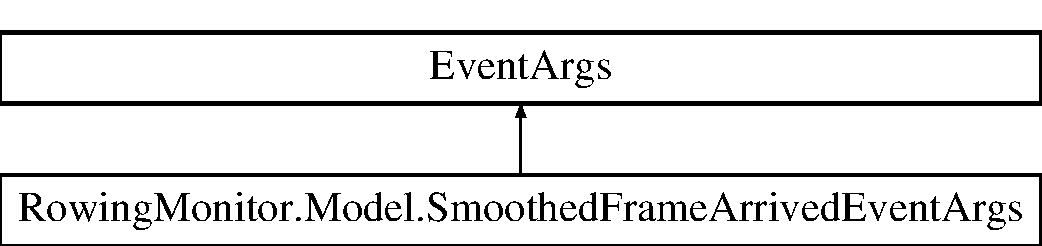
\includegraphics[height=2.000000cm]{class_rowing_monitor_1_1_model_1_1_smoothed_frame_arrived_event_args}
\end{center}
\end{figure}
\subsection*{Public Member Functions}
\begin{DoxyCompactItemize}
\item 
\hyperlink{class_rowing_monitor_1_1_model_1_1_smoothed_frame_arrived_event_args_a923725ca3400f634d0ce4a01c03388e7}{Smoothed\+Frame\+Arrived\+Event\+Args} (\hyperlink{struct_rowing_monitor_1_1_model_1_1_util_1_1_joint_data}{Joint\+Data} raw\+Joint\+Data, \hyperlink{struct_rowing_monitor_1_1_model_1_1_util_1_1_joint_data}{Joint\+Data} smoothed\+Joint\+Data)
\end{DoxyCompactItemize}
\subsection*{Properties}
\begin{DoxyCompactItemize}
\item 
\hyperlink{struct_rowing_monitor_1_1_model_1_1_util_1_1_joint_data}{Joint\+Data} \hyperlink{class_rowing_monitor_1_1_model_1_1_smoothed_frame_arrived_event_args_ae8c8a6d20114b898e9192ed282393178}{Raw\+Joint\+Data}\hspace{0.3cm}{\ttfamily  \mbox{[}get\mbox{]}}
\item 
\hyperlink{struct_rowing_monitor_1_1_model_1_1_util_1_1_joint_data}{Joint\+Data} \hyperlink{class_rowing_monitor_1_1_model_1_1_smoothed_frame_arrived_event_args_adee9a15912d769914f058a7e984948d6}{Smoothed\+Joint\+Data}\hspace{0.3cm}{\ttfamily  \mbox{[}get\mbox{]}}
\end{DoxyCompactItemize}


\subsection{Detailed Description}
Represents the arguments for a smoothed joint data arrived event. 



\subsection{Constructor \& Destructor Documentation}
\mbox{\Hypertarget{class_rowing_monitor_1_1_model_1_1_smoothed_frame_arrived_event_args_a923725ca3400f634d0ce4a01c03388e7}\label{class_rowing_monitor_1_1_model_1_1_smoothed_frame_arrived_event_args_a923725ca3400f634d0ce4a01c03388e7}} 
\index{Rowing\+Monitor\+::\+Model\+::\+Smoothed\+Frame\+Arrived\+Event\+Args@{Rowing\+Monitor\+::\+Model\+::\+Smoothed\+Frame\+Arrived\+Event\+Args}!Smoothed\+Frame\+Arrived\+Event\+Args@{Smoothed\+Frame\+Arrived\+Event\+Args}}
\index{Smoothed\+Frame\+Arrived\+Event\+Args@{Smoothed\+Frame\+Arrived\+Event\+Args}!Rowing\+Monitor\+::\+Model\+::\+Smoothed\+Frame\+Arrived\+Event\+Args@{Rowing\+Monitor\+::\+Model\+::\+Smoothed\+Frame\+Arrived\+Event\+Args}}
\subsubsection{\texorpdfstring{Smoothed\+Frame\+Arrived\+Event\+Args()}{SmoothedFrameArrivedEventArgs()}}
{\footnotesize\ttfamily Rowing\+Monitor.\+Model.\+Smoothed\+Frame\+Arrived\+Event\+Args.\+Smoothed\+Frame\+Arrived\+Event\+Args (\begin{DoxyParamCaption}\item[{\hyperlink{struct_rowing_monitor_1_1_model_1_1_util_1_1_joint_data}{Joint\+Data}}]{raw\+Joint\+Data,  }\item[{\hyperlink{struct_rowing_monitor_1_1_model_1_1_util_1_1_joint_data}{Joint\+Data}}]{smoothed\+Joint\+Data }\end{DoxyParamCaption})}



\subsection{Property Documentation}
\mbox{\Hypertarget{class_rowing_monitor_1_1_model_1_1_smoothed_frame_arrived_event_args_ae8c8a6d20114b898e9192ed282393178}\label{class_rowing_monitor_1_1_model_1_1_smoothed_frame_arrived_event_args_ae8c8a6d20114b898e9192ed282393178}} 
\index{Rowing\+Monitor\+::\+Model\+::\+Smoothed\+Frame\+Arrived\+Event\+Args@{Rowing\+Monitor\+::\+Model\+::\+Smoothed\+Frame\+Arrived\+Event\+Args}!Raw\+Joint\+Data@{Raw\+Joint\+Data}}
\index{Raw\+Joint\+Data@{Raw\+Joint\+Data}!Rowing\+Monitor\+::\+Model\+::\+Smoothed\+Frame\+Arrived\+Event\+Args@{Rowing\+Monitor\+::\+Model\+::\+Smoothed\+Frame\+Arrived\+Event\+Args}}
\subsubsection{\texorpdfstring{Raw\+Joint\+Data}{RawJointData}}
{\footnotesize\ttfamily \hyperlink{struct_rowing_monitor_1_1_model_1_1_util_1_1_joint_data}{Joint\+Data} Rowing\+Monitor.\+Model.\+Smoothed\+Frame\+Arrived\+Event\+Args.\+Raw\+Joint\+Data\hspace{0.3cm}{\ttfamily [get]}}

\mbox{\Hypertarget{class_rowing_monitor_1_1_model_1_1_smoothed_frame_arrived_event_args_adee9a15912d769914f058a7e984948d6}\label{class_rowing_monitor_1_1_model_1_1_smoothed_frame_arrived_event_args_adee9a15912d769914f058a7e984948d6}} 
\index{Rowing\+Monitor\+::\+Model\+::\+Smoothed\+Frame\+Arrived\+Event\+Args@{Rowing\+Monitor\+::\+Model\+::\+Smoothed\+Frame\+Arrived\+Event\+Args}!Smoothed\+Joint\+Data@{Smoothed\+Joint\+Data}}
\index{Smoothed\+Joint\+Data@{Smoothed\+Joint\+Data}!Rowing\+Monitor\+::\+Model\+::\+Smoothed\+Frame\+Arrived\+Event\+Args@{Rowing\+Monitor\+::\+Model\+::\+Smoothed\+Frame\+Arrived\+Event\+Args}}
\subsubsection{\texorpdfstring{Smoothed\+Joint\+Data}{SmoothedJointData}}
{\footnotesize\ttfamily \hyperlink{struct_rowing_monitor_1_1_model_1_1_util_1_1_joint_data}{Joint\+Data} Rowing\+Monitor.\+Model.\+Smoothed\+Frame\+Arrived\+Event\+Args.\+Smoothed\+Joint\+Data\hspace{0.3cm}{\ttfamily [get]}}



The documentation for this class was generated from the following file\+:\begin{DoxyCompactItemize}
\item 
Model/\+Event\+Args/\hyperlink{_smoothed_frame_arrived_event_args_8cs}{Smoothed\+Frame\+Arrived\+Event\+Args.\+cs}\end{DoxyCompactItemize}

\hypertarget{struct_rowing_monitor_1_1_model_1_1_util_1_1_subsequence}{}\section{Rowing\+Monitor.\+Model.\+Util.\+Subsequence Struct Reference}
\label{struct_rowing_monitor_1_1_model_1_1_util_1_1_subsequence}\index{Rowing\+Monitor.\+Model.\+Util.\+Subsequence@{Rowing\+Monitor.\+Model.\+Util.\+Subsequence}}


\hyperlink{struct_rowing_monitor_1_1_model_1_1_util_1_1_subsequence}{Subsequence} in a data stream which suits a given template.  


\subsection*{Properties}
\begin{DoxyCompactItemize}
\item 
double \hyperlink{struct_rowing_monitor_1_1_model_1_1_util_1_1_subsequence_a9f07ec73d4dcc7cb1d9e97f7e979fcc1}{Distance}\hspace{0.3cm}{\ttfamily  \mbox{[}get, set\mbox{]}}
\begin{DoxyCompactList}\small\item\em Calculates distance between the template and the data stream. \end{DoxyCompactList}\item 
int \hyperlink{struct_rowing_monitor_1_1_model_1_1_util_1_1_subsequence_af085c001955793f45836d6c1cf3d4882}{T\+Start}\hspace{0.3cm}{\ttfamily  \mbox{[}get, set\mbox{]}}
\begin{DoxyCompactList}\small\item\em Starttime of data stream which fits to the template. \end{DoxyCompactList}\item 
int \hyperlink{struct_rowing_monitor_1_1_model_1_1_util_1_1_subsequence_a839b2f62176c2546a8e0d42b87801954}{T\+End}\hspace{0.3cm}{\ttfamily  \mbox{[}get, set\mbox{]}}
\begin{DoxyCompactList}\small\item\em Endtime of data stream which fits to the template. \end{DoxyCompactList}\item 
\hyperlink{namespace_rowing_monitor_1_1_model_1_1_util_a248a257b884983ed79c45a8b34ee9580}{Subsequence\+Status} \hyperlink{struct_rowing_monitor_1_1_model_1_1_util_1_1_subsequence_a437775e5f7ee4b63b6a33a01ef46bf0c}{Status}\hspace{0.3cm}{\ttfamily  \mbox{[}get, set\mbox{]}}
\begin{DoxyCompactList}\small\item\em Status of detected subsequence. \end{DoxyCompactList}\item 
int \hyperlink{struct_rowing_monitor_1_1_model_1_1_util_1_1_subsequence_aaaed8840b79d2c683073ecf408bc6d51}{T\+Detected}\hspace{0.3cm}{\ttfamily  \mbox{[}get, set\mbox{]}}
\begin{DoxyCompactList}\small\item\em Time of detection. \end{DoxyCompactList}\end{DoxyCompactItemize}


\subsection{Detailed Description}
\hyperlink{struct_rowing_monitor_1_1_model_1_1_util_1_1_subsequence}{Subsequence} in a data stream which suits a given template. 



\subsection{Property Documentation}
\mbox{\Hypertarget{struct_rowing_monitor_1_1_model_1_1_util_1_1_subsequence_a9f07ec73d4dcc7cb1d9e97f7e979fcc1}\label{struct_rowing_monitor_1_1_model_1_1_util_1_1_subsequence_a9f07ec73d4dcc7cb1d9e97f7e979fcc1}} 
\index{Rowing\+Monitor\+::\+Model\+::\+Util\+::\+Subsequence@{Rowing\+Monitor\+::\+Model\+::\+Util\+::\+Subsequence}!Distance@{Distance}}
\index{Distance@{Distance}!Rowing\+Monitor\+::\+Model\+::\+Util\+::\+Subsequence@{Rowing\+Monitor\+::\+Model\+::\+Util\+::\+Subsequence}}
\subsubsection{\texorpdfstring{Distance}{Distance}}
{\footnotesize\ttfamily double Rowing\+Monitor.\+Model.\+Util.\+Subsequence.\+Distance\hspace{0.3cm}{\ttfamily [get]}, {\ttfamily [set]}}



Calculates distance between the template and the data stream. 

\mbox{\Hypertarget{struct_rowing_monitor_1_1_model_1_1_util_1_1_subsequence_a437775e5f7ee4b63b6a33a01ef46bf0c}\label{struct_rowing_monitor_1_1_model_1_1_util_1_1_subsequence_a437775e5f7ee4b63b6a33a01ef46bf0c}} 
\index{Rowing\+Monitor\+::\+Model\+::\+Util\+::\+Subsequence@{Rowing\+Monitor\+::\+Model\+::\+Util\+::\+Subsequence}!Status@{Status}}
\index{Status@{Status}!Rowing\+Monitor\+::\+Model\+::\+Util\+::\+Subsequence@{Rowing\+Monitor\+::\+Model\+::\+Util\+::\+Subsequence}}
\subsubsection{\texorpdfstring{Status}{Status}}
{\footnotesize\ttfamily \hyperlink{namespace_rowing_monitor_1_1_model_1_1_util_a248a257b884983ed79c45a8b34ee9580}{Subsequence\+Status} Rowing\+Monitor.\+Model.\+Util.\+Subsequence.\+Status\hspace{0.3cm}{\ttfamily [get]}, {\ttfamily [set]}}



Status of detected subsequence. 

\mbox{\Hypertarget{struct_rowing_monitor_1_1_model_1_1_util_1_1_subsequence_aaaed8840b79d2c683073ecf408bc6d51}\label{struct_rowing_monitor_1_1_model_1_1_util_1_1_subsequence_aaaed8840b79d2c683073ecf408bc6d51}} 
\index{Rowing\+Monitor\+::\+Model\+::\+Util\+::\+Subsequence@{Rowing\+Monitor\+::\+Model\+::\+Util\+::\+Subsequence}!T\+Detected@{T\+Detected}}
\index{T\+Detected@{T\+Detected}!Rowing\+Monitor\+::\+Model\+::\+Util\+::\+Subsequence@{Rowing\+Monitor\+::\+Model\+::\+Util\+::\+Subsequence}}
\subsubsection{\texorpdfstring{T\+Detected}{TDetected}}
{\footnotesize\ttfamily int Rowing\+Monitor.\+Model.\+Util.\+Subsequence.\+T\+Detected\hspace{0.3cm}{\ttfamily [get]}, {\ttfamily [set]}}



Time of detection. 

\mbox{\Hypertarget{struct_rowing_monitor_1_1_model_1_1_util_1_1_subsequence_a839b2f62176c2546a8e0d42b87801954}\label{struct_rowing_monitor_1_1_model_1_1_util_1_1_subsequence_a839b2f62176c2546a8e0d42b87801954}} 
\index{Rowing\+Monitor\+::\+Model\+::\+Util\+::\+Subsequence@{Rowing\+Monitor\+::\+Model\+::\+Util\+::\+Subsequence}!T\+End@{T\+End}}
\index{T\+End@{T\+End}!Rowing\+Monitor\+::\+Model\+::\+Util\+::\+Subsequence@{Rowing\+Monitor\+::\+Model\+::\+Util\+::\+Subsequence}}
\subsubsection{\texorpdfstring{T\+End}{TEnd}}
{\footnotesize\ttfamily int Rowing\+Monitor.\+Model.\+Util.\+Subsequence.\+T\+End\hspace{0.3cm}{\ttfamily [get]}, {\ttfamily [set]}}



Endtime of data stream which fits to the template. 

\mbox{\Hypertarget{struct_rowing_monitor_1_1_model_1_1_util_1_1_subsequence_af085c001955793f45836d6c1cf3d4882}\label{struct_rowing_monitor_1_1_model_1_1_util_1_1_subsequence_af085c001955793f45836d6c1cf3d4882}} 
\index{Rowing\+Monitor\+::\+Model\+::\+Util\+::\+Subsequence@{Rowing\+Monitor\+::\+Model\+::\+Util\+::\+Subsequence}!T\+Start@{T\+Start}}
\index{T\+Start@{T\+Start}!Rowing\+Monitor\+::\+Model\+::\+Util\+::\+Subsequence@{Rowing\+Monitor\+::\+Model\+::\+Util\+::\+Subsequence}}
\subsubsection{\texorpdfstring{T\+Start}{TStart}}
{\footnotesize\ttfamily int Rowing\+Monitor.\+Model.\+Util.\+Subsequence.\+T\+Start\hspace{0.3cm}{\ttfamily [get]}, {\ttfamily [set]}}



Starttime of data stream which fits to the template. 



The documentation for this struct was generated from the following file\+:\begin{DoxyCompactItemize}
\item 
Model/\+Util/\hyperlink{_subsequence_d_t_w_8cs}{Subsequence\+D\+T\+W.\+cs}\end{DoxyCompactItemize}

\hypertarget{class_rowing_monitor_1_1_model_1_1_util_1_1_subsequence_d_t_w}{}\section{Rowing\+Monitor.\+Model.\+Util.\+Subsequence\+D\+TW Class Reference}
\label{class_rowing_monitor_1_1_model_1_1_util_1_1_subsequence_d_t_w}\index{Rowing\+Monitor.\+Model.\+Util.\+Subsequence\+D\+TW@{Rowing\+Monitor.\+Model.\+Util.\+Subsequence\+D\+TW}}


Compares an online data stream with a template stream. Uses the S\+P\+R\+I\+NG D\+TW algorithm.  


\subsection*{Public Member Functions}
\begin{DoxyCompactItemize}
\item 
\hyperlink{class_rowing_monitor_1_1_model_1_1_util_1_1_subsequence_d_t_w_a16ee898f6e11aee3d1b3ccfb482cdddb}{Subsequence\+D\+TW} (List$<$ double $>$ template, float distance\+Threshold, int minimum\+Subsequence\+Length=2)
\begin{DoxyCompactList}\small\item\em Creates a new instance of the \hyperlink{class_rowing_monitor_1_1_model_1_1_util_1_1_subsequence_d_t_w}{Subsequence\+D\+TW} class. \end{DoxyCompactList}\item 
\hyperlink{struct_rowing_monitor_1_1_model_1_1_util_1_1_subsequence}{Subsequence} \hyperlink{class_rowing_monitor_1_1_model_1_1_util_1_1_subsequence_d_t_w_a2aa9afce49cbb11a86ee3e5791397416}{compare\+Data\+Stream} (double xT, int t)
\begin{DoxyCompactList}\small\item\em Compare the value x at time t of the data stream with the template. Returns an unset, not optimal or optimal subsequence with its distance, starttime and endtime. Uses the S\+P\+R\+I\+NG D\+TW algorithm. \end{DoxyCompactList}\end{DoxyCompactItemize}


\subsection{Detailed Description}
Compares an online data stream with a template stream. Uses the S\+P\+R\+I\+NG D\+TW algorithm. 



\subsection{Constructor \& Destructor Documentation}
\mbox{\Hypertarget{class_rowing_monitor_1_1_model_1_1_util_1_1_subsequence_d_t_w_a16ee898f6e11aee3d1b3ccfb482cdddb}\label{class_rowing_monitor_1_1_model_1_1_util_1_1_subsequence_d_t_w_a16ee898f6e11aee3d1b3ccfb482cdddb}} 
\index{Rowing\+Monitor\+::\+Model\+::\+Util\+::\+Subsequence\+D\+TW@{Rowing\+Monitor\+::\+Model\+::\+Util\+::\+Subsequence\+D\+TW}!Subsequence\+D\+TW@{Subsequence\+D\+TW}}
\index{Subsequence\+D\+TW@{Subsequence\+D\+TW}!Rowing\+Monitor\+::\+Model\+::\+Util\+::\+Subsequence\+D\+TW@{Rowing\+Monitor\+::\+Model\+::\+Util\+::\+Subsequence\+D\+TW}}
\subsubsection{\texorpdfstring{Subsequence\+D\+T\+W()}{SubsequenceDTW()}}
{\footnotesize\ttfamily Rowing\+Monitor.\+Model.\+Util.\+Subsequence\+D\+T\+W.\+Subsequence\+D\+TW (\begin{DoxyParamCaption}\item[{List$<$ double $>$}]{template,  }\item[{float}]{distance\+Threshold,  }\item[{int}]{minimum\+Subsequence\+Length = {\ttfamily 2} }\end{DoxyParamCaption})}



Creates a new instance of the \hyperlink{class_rowing_monitor_1_1_model_1_1_util_1_1_subsequence_d_t_w}{Subsequence\+D\+TW} class. 


\begin{DoxyParams}{Parameters}
{\em template} & \\
\hline
\end{DoxyParams}
Template stream for comparison. 
\begin{DoxyParams}{Parameters}
{\em distance\+Threshold} & \\
\hline
\end{DoxyParams}
Distance threshold which describes the maximum distance that reports a detected subsequence. 
\begin{DoxyParams}{Parameters}
{\em minimum\+Subsequence\+Length} & \\
\hline
\end{DoxyParams}
Minimum length of a detected subsequence. 

\subsection{Member Function Documentation}
\mbox{\Hypertarget{class_rowing_monitor_1_1_model_1_1_util_1_1_subsequence_d_t_w_a2aa9afce49cbb11a86ee3e5791397416}\label{class_rowing_monitor_1_1_model_1_1_util_1_1_subsequence_d_t_w_a2aa9afce49cbb11a86ee3e5791397416}} 
\index{Rowing\+Monitor\+::\+Model\+::\+Util\+::\+Subsequence\+D\+TW@{Rowing\+Monitor\+::\+Model\+::\+Util\+::\+Subsequence\+D\+TW}!compare\+Data\+Stream@{compare\+Data\+Stream}}
\index{compare\+Data\+Stream@{compare\+Data\+Stream}!Rowing\+Monitor\+::\+Model\+::\+Util\+::\+Subsequence\+D\+TW@{Rowing\+Monitor\+::\+Model\+::\+Util\+::\+Subsequence\+D\+TW}}
\subsubsection{\texorpdfstring{compare\+Data\+Stream()}{compareDataStream()}}
{\footnotesize\ttfamily \hyperlink{struct_rowing_monitor_1_1_model_1_1_util_1_1_subsequence}{Subsequence} Rowing\+Monitor.\+Model.\+Util.\+Subsequence\+D\+T\+W.\+compare\+Data\+Stream (\begin{DoxyParamCaption}\item[{double}]{xT,  }\item[{int}]{t }\end{DoxyParamCaption})}



Compare the value x at time t of the data stream with the template. Returns an unset, not optimal or optimal subsequence with its distance, starttime and endtime. Uses the S\+P\+R\+I\+NG D\+TW algorithm. 


\begin{DoxyParams}{Parameters}
{\em xT} & \\
\hline
\end{DoxyParams}
Value x of data stream at time t. 
\begin{DoxyParams}{Parameters}
{\em t} & \\
\hline
\end{DoxyParams}
Time t of value x. Time starts with 1. \begin{DoxyReturn}{Returns}

\end{DoxyReturn}
A subsequence with its distance, starttime and endtime. 

The documentation for this class was generated from the following file\+:\begin{DoxyCompactItemize}
\item 
Model/\+Util/\hyperlink{_subsequence_d_t_w_8cs}{Subsequence\+D\+T\+W.\+cs}\end{DoxyCompactItemize}

\hypertarget{struct_rowing_monitor_1_1_model_1_1_pipeline_1_1_kinect_joint_filter_1_1_t_r_a_n_s_f_o_r_m___s_m_o_o_t_h___p_a_r_a_m_e_t_e_r_s}{}\section{Rowing\+Monitor.\+Model.\+Pipeline.\+Kinect\+Joint\+Filter.\+T\+R\+A\+N\+S\+F\+O\+R\+M\+\_\+\+S\+M\+O\+O\+T\+H\+\_\+\+P\+A\+R\+A\+M\+E\+T\+E\+RS Struct Reference}
\label{struct_rowing_monitor_1_1_model_1_1_pipeline_1_1_kinect_joint_filter_1_1_t_r_a_n_s_f_o_r_m___s_m_o_o_t_h___p_a_r_a_m_e_t_e_r_s}\index{Rowing\+Monitor.\+Model.\+Pipeline.\+Kinect\+Joint\+Filter.\+T\+R\+A\+N\+S\+F\+O\+R\+M\+\_\+\+S\+M\+O\+O\+T\+H\+\_\+\+P\+A\+R\+A\+M\+E\+T\+E\+RS@{Rowing\+Monitor.\+Model.\+Pipeline.\+Kinect\+Joint\+Filter.\+T\+R\+A\+N\+S\+F\+O\+R\+M\+\_\+\+S\+M\+O\+O\+T\+H\+\_\+\+P\+A\+R\+A\+M\+E\+T\+E\+RS}}
\subsection*{Public Attributes}
\begin{DoxyCompactItemize}
\item 
float \hyperlink{struct_rowing_monitor_1_1_model_1_1_pipeline_1_1_kinect_joint_filter_1_1_t_r_a_n_s_f_o_r_m___s_m_o_o_t_h___p_a_r_a_m_e_t_e_r_s_a3df04b87ddfcaabc9b88f91270460add}{f\+Smoothing}
\item 
float \hyperlink{struct_rowing_monitor_1_1_model_1_1_pipeline_1_1_kinect_joint_filter_1_1_t_r_a_n_s_f_o_r_m___s_m_o_o_t_h___p_a_r_a_m_e_t_e_r_s_a9d5f856bec242947352351a8e60560ce}{f\+Correction}
\item 
float \hyperlink{struct_rowing_monitor_1_1_model_1_1_pipeline_1_1_kinect_joint_filter_1_1_t_r_a_n_s_f_o_r_m___s_m_o_o_t_h___p_a_r_a_m_e_t_e_r_s_a7333c909fc6d7470548c458ddd01b259}{f\+Prediction}
\item 
float \hyperlink{struct_rowing_monitor_1_1_model_1_1_pipeline_1_1_kinect_joint_filter_1_1_t_r_a_n_s_f_o_r_m___s_m_o_o_t_h___p_a_r_a_m_e_t_e_r_s_a336103e401e4fce01b7c5a9368908414}{f\+Jitter\+Radius}
\item 
float \hyperlink{struct_rowing_monitor_1_1_model_1_1_pipeline_1_1_kinect_joint_filter_1_1_t_r_a_n_s_f_o_r_m___s_m_o_o_t_h___p_a_r_a_m_e_t_e_r_s_a2c603efc3e88f34da44904f19060e9f1}{f\+Max\+Deviation\+Radius}
\end{DoxyCompactItemize}


\subsection{Member Data Documentation}
\mbox{\Hypertarget{struct_rowing_monitor_1_1_model_1_1_pipeline_1_1_kinect_joint_filter_1_1_t_r_a_n_s_f_o_r_m___s_m_o_o_t_h___p_a_r_a_m_e_t_e_r_s_a9d5f856bec242947352351a8e60560ce}\label{struct_rowing_monitor_1_1_model_1_1_pipeline_1_1_kinect_joint_filter_1_1_t_r_a_n_s_f_o_r_m___s_m_o_o_t_h___p_a_r_a_m_e_t_e_r_s_a9d5f856bec242947352351a8e60560ce}} 
\index{Rowing\+Monitor\+::\+Model\+::\+Pipeline\+::\+Kinect\+Joint\+Filter\+::\+T\+R\+A\+N\+S\+F\+O\+R\+M\+\_\+\+S\+M\+O\+O\+T\+H\+\_\+\+P\+A\+R\+A\+M\+E\+T\+E\+RS@{Rowing\+Monitor\+::\+Model\+::\+Pipeline\+::\+Kinect\+Joint\+Filter\+::\+T\+R\+A\+N\+S\+F\+O\+R\+M\+\_\+\+S\+M\+O\+O\+T\+H\+\_\+\+P\+A\+R\+A\+M\+E\+T\+E\+RS}!f\+Correction@{f\+Correction}}
\index{f\+Correction@{f\+Correction}!Rowing\+Monitor\+::\+Model\+::\+Pipeline\+::\+Kinect\+Joint\+Filter\+::\+T\+R\+A\+N\+S\+F\+O\+R\+M\+\_\+\+S\+M\+O\+O\+T\+H\+\_\+\+P\+A\+R\+A\+M\+E\+T\+E\+RS@{Rowing\+Monitor\+::\+Model\+::\+Pipeline\+::\+Kinect\+Joint\+Filter\+::\+T\+R\+A\+N\+S\+F\+O\+R\+M\+\_\+\+S\+M\+O\+O\+T\+H\+\_\+\+P\+A\+R\+A\+M\+E\+T\+E\+RS}}
\subsubsection{\texorpdfstring{f\+Correction}{fCorrection}}
{\footnotesize\ttfamily float Rowing\+Monitor.\+Model.\+Pipeline.\+Kinect\+Joint\+Filter.\+T\+R\+A\+N\+S\+F\+O\+R\+M\+\_\+\+S\+M\+O\+O\+T\+H\+\_\+\+P\+A\+R\+A\+M\+E\+T\+E\+R\+S.\+f\+Correction}

\mbox{\Hypertarget{struct_rowing_monitor_1_1_model_1_1_pipeline_1_1_kinect_joint_filter_1_1_t_r_a_n_s_f_o_r_m___s_m_o_o_t_h___p_a_r_a_m_e_t_e_r_s_a336103e401e4fce01b7c5a9368908414}\label{struct_rowing_monitor_1_1_model_1_1_pipeline_1_1_kinect_joint_filter_1_1_t_r_a_n_s_f_o_r_m___s_m_o_o_t_h___p_a_r_a_m_e_t_e_r_s_a336103e401e4fce01b7c5a9368908414}} 
\index{Rowing\+Monitor\+::\+Model\+::\+Pipeline\+::\+Kinect\+Joint\+Filter\+::\+T\+R\+A\+N\+S\+F\+O\+R\+M\+\_\+\+S\+M\+O\+O\+T\+H\+\_\+\+P\+A\+R\+A\+M\+E\+T\+E\+RS@{Rowing\+Monitor\+::\+Model\+::\+Pipeline\+::\+Kinect\+Joint\+Filter\+::\+T\+R\+A\+N\+S\+F\+O\+R\+M\+\_\+\+S\+M\+O\+O\+T\+H\+\_\+\+P\+A\+R\+A\+M\+E\+T\+E\+RS}!f\+Jitter\+Radius@{f\+Jitter\+Radius}}
\index{f\+Jitter\+Radius@{f\+Jitter\+Radius}!Rowing\+Monitor\+::\+Model\+::\+Pipeline\+::\+Kinect\+Joint\+Filter\+::\+T\+R\+A\+N\+S\+F\+O\+R\+M\+\_\+\+S\+M\+O\+O\+T\+H\+\_\+\+P\+A\+R\+A\+M\+E\+T\+E\+RS@{Rowing\+Monitor\+::\+Model\+::\+Pipeline\+::\+Kinect\+Joint\+Filter\+::\+T\+R\+A\+N\+S\+F\+O\+R\+M\+\_\+\+S\+M\+O\+O\+T\+H\+\_\+\+P\+A\+R\+A\+M\+E\+T\+E\+RS}}
\subsubsection{\texorpdfstring{f\+Jitter\+Radius}{fJitterRadius}}
{\footnotesize\ttfamily float Rowing\+Monitor.\+Model.\+Pipeline.\+Kinect\+Joint\+Filter.\+T\+R\+A\+N\+S\+F\+O\+R\+M\+\_\+\+S\+M\+O\+O\+T\+H\+\_\+\+P\+A\+R\+A\+M\+E\+T\+E\+R\+S.\+f\+Jitter\+Radius}

\mbox{\Hypertarget{struct_rowing_monitor_1_1_model_1_1_pipeline_1_1_kinect_joint_filter_1_1_t_r_a_n_s_f_o_r_m___s_m_o_o_t_h___p_a_r_a_m_e_t_e_r_s_a2c603efc3e88f34da44904f19060e9f1}\label{struct_rowing_monitor_1_1_model_1_1_pipeline_1_1_kinect_joint_filter_1_1_t_r_a_n_s_f_o_r_m___s_m_o_o_t_h___p_a_r_a_m_e_t_e_r_s_a2c603efc3e88f34da44904f19060e9f1}} 
\index{Rowing\+Monitor\+::\+Model\+::\+Pipeline\+::\+Kinect\+Joint\+Filter\+::\+T\+R\+A\+N\+S\+F\+O\+R\+M\+\_\+\+S\+M\+O\+O\+T\+H\+\_\+\+P\+A\+R\+A\+M\+E\+T\+E\+RS@{Rowing\+Monitor\+::\+Model\+::\+Pipeline\+::\+Kinect\+Joint\+Filter\+::\+T\+R\+A\+N\+S\+F\+O\+R\+M\+\_\+\+S\+M\+O\+O\+T\+H\+\_\+\+P\+A\+R\+A\+M\+E\+T\+E\+RS}!f\+Max\+Deviation\+Radius@{f\+Max\+Deviation\+Radius}}
\index{f\+Max\+Deviation\+Radius@{f\+Max\+Deviation\+Radius}!Rowing\+Monitor\+::\+Model\+::\+Pipeline\+::\+Kinect\+Joint\+Filter\+::\+T\+R\+A\+N\+S\+F\+O\+R\+M\+\_\+\+S\+M\+O\+O\+T\+H\+\_\+\+P\+A\+R\+A\+M\+E\+T\+E\+RS@{Rowing\+Monitor\+::\+Model\+::\+Pipeline\+::\+Kinect\+Joint\+Filter\+::\+T\+R\+A\+N\+S\+F\+O\+R\+M\+\_\+\+S\+M\+O\+O\+T\+H\+\_\+\+P\+A\+R\+A\+M\+E\+T\+E\+RS}}
\subsubsection{\texorpdfstring{f\+Max\+Deviation\+Radius}{fMaxDeviationRadius}}
{\footnotesize\ttfamily float Rowing\+Monitor.\+Model.\+Pipeline.\+Kinect\+Joint\+Filter.\+T\+R\+A\+N\+S\+F\+O\+R\+M\+\_\+\+S\+M\+O\+O\+T\+H\+\_\+\+P\+A\+R\+A\+M\+E\+T\+E\+R\+S.\+f\+Max\+Deviation\+Radius}

\mbox{\Hypertarget{struct_rowing_monitor_1_1_model_1_1_pipeline_1_1_kinect_joint_filter_1_1_t_r_a_n_s_f_o_r_m___s_m_o_o_t_h___p_a_r_a_m_e_t_e_r_s_a7333c909fc6d7470548c458ddd01b259}\label{struct_rowing_monitor_1_1_model_1_1_pipeline_1_1_kinect_joint_filter_1_1_t_r_a_n_s_f_o_r_m___s_m_o_o_t_h___p_a_r_a_m_e_t_e_r_s_a7333c909fc6d7470548c458ddd01b259}} 
\index{Rowing\+Monitor\+::\+Model\+::\+Pipeline\+::\+Kinect\+Joint\+Filter\+::\+T\+R\+A\+N\+S\+F\+O\+R\+M\+\_\+\+S\+M\+O\+O\+T\+H\+\_\+\+P\+A\+R\+A\+M\+E\+T\+E\+RS@{Rowing\+Monitor\+::\+Model\+::\+Pipeline\+::\+Kinect\+Joint\+Filter\+::\+T\+R\+A\+N\+S\+F\+O\+R\+M\+\_\+\+S\+M\+O\+O\+T\+H\+\_\+\+P\+A\+R\+A\+M\+E\+T\+E\+RS}!f\+Prediction@{f\+Prediction}}
\index{f\+Prediction@{f\+Prediction}!Rowing\+Monitor\+::\+Model\+::\+Pipeline\+::\+Kinect\+Joint\+Filter\+::\+T\+R\+A\+N\+S\+F\+O\+R\+M\+\_\+\+S\+M\+O\+O\+T\+H\+\_\+\+P\+A\+R\+A\+M\+E\+T\+E\+RS@{Rowing\+Monitor\+::\+Model\+::\+Pipeline\+::\+Kinect\+Joint\+Filter\+::\+T\+R\+A\+N\+S\+F\+O\+R\+M\+\_\+\+S\+M\+O\+O\+T\+H\+\_\+\+P\+A\+R\+A\+M\+E\+T\+E\+RS}}
\subsubsection{\texorpdfstring{f\+Prediction}{fPrediction}}
{\footnotesize\ttfamily float Rowing\+Monitor.\+Model.\+Pipeline.\+Kinect\+Joint\+Filter.\+T\+R\+A\+N\+S\+F\+O\+R\+M\+\_\+\+S\+M\+O\+O\+T\+H\+\_\+\+P\+A\+R\+A\+M\+E\+T\+E\+R\+S.\+f\+Prediction}

\mbox{\Hypertarget{struct_rowing_monitor_1_1_model_1_1_pipeline_1_1_kinect_joint_filter_1_1_t_r_a_n_s_f_o_r_m___s_m_o_o_t_h___p_a_r_a_m_e_t_e_r_s_a3df04b87ddfcaabc9b88f91270460add}\label{struct_rowing_monitor_1_1_model_1_1_pipeline_1_1_kinect_joint_filter_1_1_t_r_a_n_s_f_o_r_m___s_m_o_o_t_h___p_a_r_a_m_e_t_e_r_s_a3df04b87ddfcaabc9b88f91270460add}} 
\index{Rowing\+Monitor\+::\+Model\+::\+Pipeline\+::\+Kinect\+Joint\+Filter\+::\+T\+R\+A\+N\+S\+F\+O\+R\+M\+\_\+\+S\+M\+O\+O\+T\+H\+\_\+\+P\+A\+R\+A\+M\+E\+T\+E\+RS@{Rowing\+Monitor\+::\+Model\+::\+Pipeline\+::\+Kinect\+Joint\+Filter\+::\+T\+R\+A\+N\+S\+F\+O\+R\+M\+\_\+\+S\+M\+O\+O\+T\+H\+\_\+\+P\+A\+R\+A\+M\+E\+T\+E\+RS}!f\+Smoothing@{f\+Smoothing}}
\index{f\+Smoothing@{f\+Smoothing}!Rowing\+Monitor\+::\+Model\+::\+Pipeline\+::\+Kinect\+Joint\+Filter\+::\+T\+R\+A\+N\+S\+F\+O\+R\+M\+\_\+\+S\+M\+O\+O\+T\+H\+\_\+\+P\+A\+R\+A\+M\+E\+T\+E\+RS@{Rowing\+Monitor\+::\+Model\+::\+Pipeline\+::\+Kinect\+Joint\+Filter\+::\+T\+R\+A\+N\+S\+F\+O\+R\+M\+\_\+\+S\+M\+O\+O\+T\+H\+\_\+\+P\+A\+R\+A\+M\+E\+T\+E\+RS}}
\subsubsection{\texorpdfstring{f\+Smoothing}{fSmoothing}}
{\footnotesize\ttfamily float Rowing\+Monitor.\+Model.\+Pipeline.\+Kinect\+Joint\+Filter.\+T\+R\+A\+N\+S\+F\+O\+R\+M\+\_\+\+S\+M\+O\+O\+T\+H\+\_\+\+P\+A\+R\+A\+M\+E\+T\+E\+R\+S.\+f\+Smoothing}



The documentation for this struct was generated from the following file\+:\begin{DoxyCompactItemize}
\item 
Model/\+Pipeline/\hyperlink{_kinect_joint_filter_8cs}{Kinect\+Joint\+Filter.\+cs}\end{DoxyCompactItemize}

\hypertarget{class_rowing_monitor_1_1_model_1_1_velocity_calculator}{}\section{Rowing\+Monitor.\+Model.\+Velocity\+Calculator Class Reference}
\label{class_rowing_monitor_1_1_model_1_1_velocity_calculator}\index{Rowing\+Monitor.\+Model.\+Velocity\+Calculator@{Rowing\+Monitor.\+Model.\+Velocity\+Calculator}}
\subsection*{Public Member Functions}
\begin{DoxyCompactItemize}
\item 
delegate void \hyperlink{class_rowing_monitor_1_1_model_1_1_velocity_calculator_aba102b7d4623af9933bfe091c2ad1d9b}{Calculated\+Frame\+Arrived\+Event\+Handler} (Object sender, \hyperlink{class_rowing_monitor_1_1_model_1_1_calculated_frame_arrived_event_args}{Calculated\+Frame\+Arrived\+Event\+Args} e)
\item 
void \hyperlink{class_rowing_monitor_1_1_model_1_1_velocity_calculator_a49c8bd67bb150dbd6e1e7c3ed31dc699}{Calculate\+Velocity} (\hyperlink{struct_rowing_monitor_1_1_model_1_1_util_1_1_joint_data}{Joint\+Data} joint\+Data)
\begin{DoxyCompactList}\small\item\em Calculates the velocity as 1st derivative (gradient) of position. Calculation needs one frame as buffer. \end{DoxyCompactList}\end{DoxyCompactItemize}
\subsection*{Events}
\begin{DoxyCompactItemize}
\item 
\hyperlink{class_rowing_monitor_1_1_model_1_1_velocity_calculator_aba102b7d4623af9933bfe091c2ad1d9b}{Calculated\+Frame\+Arrived\+Event\+Handler} \hyperlink{class_rowing_monitor_1_1_model_1_1_velocity_calculator_a0da4ec78b2279bb46e43c9e35914e573}{Calculated\+Frame\+Arrived}
\end{DoxyCompactItemize}


\subsection{Member Function Documentation}
\mbox{\Hypertarget{class_rowing_monitor_1_1_model_1_1_velocity_calculator_aba102b7d4623af9933bfe091c2ad1d9b}\label{class_rowing_monitor_1_1_model_1_1_velocity_calculator_aba102b7d4623af9933bfe091c2ad1d9b}} 
\index{Rowing\+Monitor\+::\+Model\+::\+Velocity\+Calculator@{Rowing\+Monitor\+::\+Model\+::\+Velocity\+Calculator}!Calculated\+Frame\+Arrived\+Event\+Handler@{Calculated\+Frame\+Arrived\+Event\+Handler}}
\index{Calculated\+Frame\+Arrived\+Event\+Handler@{Calculated\+Frame\+Arrived\+Event\+Handler}!Rowing\+Monitor\+::\+Model\+::\+Velocity\+Calculator@{Rowing\+Monitor\+::\+Model\+::\+Velocity\+Calculator}}
\subsubsection{\texorpdfstring{Calculated\+Frame\+Arrived\+Event\+Handler()}{CalculatedFrameArrivedEventHandler()}}
{\footnotesize\ttfamily delegate void Rowing\+Monitor.\+Model.\+Velocity\+Calculator.\+Calculated\+Frame\+Arrived\+Event\+Handler (\begin{DoxyParamCaption}\item[{Object}]{sender,  }\item[{\hyperlink{class_rowing_monitor_1_1_model_1_1_calculated_frame_arrived_event_args}{Calculated\+Frame\+Arrived\+Event\+Args}}]{e }\end{DoxyParamCaption})}

\mbox{\Hypertarget{class_rowing_monitor_1_1_model_1_1_velocity_calculator_a49c8bd67bb150dbd6e1e7c3ed31dc699}\label{class_rowing_monitor_1_1_model_1_1_velocity_calculator_a49c8bd67bb150dbd6e1e7c3ed31dc699}} 
\index{Rowing\+Monitor\+::\+Model\+::\+Velocity\+Calculator@{Rowing\+Monitor\+::\+Model\+::\+Velocity\+Calculator}!Calculate\+Velocity@{Calculate\+Velocity}}
\index{Calculate\+Velocity@{Calculate\+Velocity}!Rowing\+Monitor\+::\+Model\+::\+Velocity\+Calculator@{Rowing\+Monitor\+::\+Model\+::\+Velocity\+Calculator}}
\subsubsection{\texorpdfstring{Calculate\+Velocity()}{CalculateVelocity()}}
{\footnotesize\ttfamily void Rowing\+Monitor.\+Model.\+Velocity\+Calculator.\+Calculate\+Velocity (\begin{DoxyParamCaption}\item[{\hyperlink{struct_rowing_monitor_1_1_model_1_1_util_1_1_joint_data}{Joint\+Data}}]{joint\+Data }\end{DoxyParamCaption})}



Calculates the velocity as 1st derivative (gradient) of position. Calculation needs one frame as buffer. 


\begin{DoxyParams}{Parameters}
{\em joint\+Data} & \\
\hline
\end{DoxyParams}


\subsection{Event Documentation}
\mbox{\Hypertarget{class_rowing_monitor_1_1_model_1_1_velocity_calculator_a0da4ec78b2279bb46e43c9e35914e573}\label{class_rowing_monitor_1_1_model_1_1_velocity_calculator_a0da4ec78b2279bb46e43c9e35914e573}} 
\index{Rowing\+Monitor\+::\+Model\+::\+Velocity\+Calculator@{Rowing\+Monitor\+::\+Model\+::\+Velocity\+Calculator}!Calculated\+Frame\+Arrived@{Calculated\+Frame\+Arrived}}
\index{Calculated\+Frame\+Arrived@{Calculated\+Frame\+Arrived}!Rowing\+Monitor\+::\+Model\+::\+Velocity\+Calculator@{Rowing\+Monitor\+::\+Model\+::\+Velocity\+Calculator}}
\subsubsection{\texorpdfstring{Calculated\+Frame\+Arrived}{CalculatedFrameArrived}}
{\footnotesize\ttfamily \hyperlink{class_rowing_monitor_1_1_model_1_1_velocity_calculator_aba102b7d4623af9933bfe091c2ad1d9b}{Calculated\+Frame\+Arrived\+Event\+Handler} Rowing\+Monitor.\+Model.\+Velocity\+Calculator.\+Calculated\+Frame\+Arrived}



The documentation for this class was generated from the following file\+:\begin{DoxyCompactItemize}
\item 
Model/\+Pipeline/\hyperlink{_velocity_calculator_8cs}{Velocity\+Calculator.\+cs}\end{DoxyCompactItemize}

\hypertarget{class_rowing_monitor_1_1_model_1_1_pipeline_1_1_z_v_c_segment_detector}{}\section{Rowing\+Monitor.\+Model.\+Pipeline.\+Z\+V\+C\+Segment\+Detector Class Reference}
\label{class_rowing_monitor_1_1_model_1_1_pipeline_1_1_z_v_c_segment_detector}\index{Rowing\+Monitor.\+Model.\+Pipeline.\+Z\+V\+C\+Segment\+Detector@{Rowing\+Monitor.\+Model.\+Pipeline.\+Z\+V\+C\+Segment\+Detector}}
Inheritance diagram for Rowing\+Monitor.\+Model.\+Pipeline.\+Z\+V\+C\+Segment\+Detector\+:\begin{figure}[H]
\begin{center}
\leavevmode
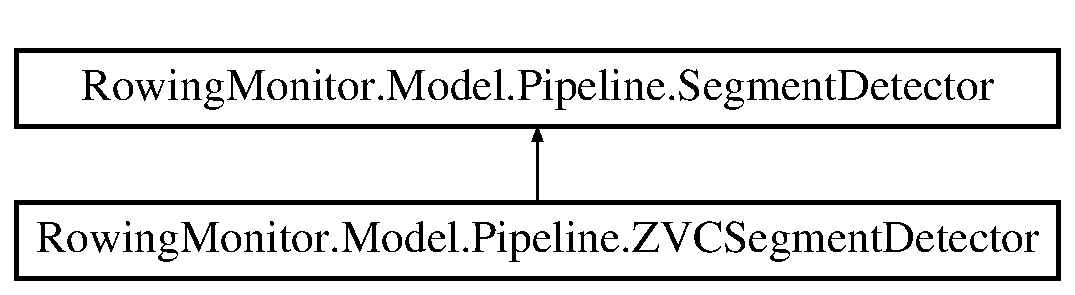
\includegraphics[height=2.000000cm]{class_rowing_monitor_1_1_model_1_1_pipeline_1_1_z_v_c_segment_detector}
\end{center}
\end{figure}
\subsection*{Public Member Functions}
\begin{DoxyCompactItemize}
\item 
\hyperlink{class_rowing_monitor_1_1_model_1_1_pipeline_1_1_z_v_c_segment_detector_ae8612877f3f7310db743529f61547616}{Z\+V\+C\+Segment\+Detector} (int minimum\+Hit\+Gap, bool start\+Segment\+With\+Rising\+Velocity=true)
\begin{DoxyCompactList}\small\item\em Creates a new zero velocity segment detector. \end{DoxyCompactList}\item 
override void \hyperlink{class_rowing_monitor_1_1_model_1_1_pipeline_1_1_z_v_c_segment_detector_a81c28e4ede1561c2fe1eca29f63f0767}{Update} (\hyperlink{struct_rowing_monitor_1_1_model_1_1_util_1_1_joint_data}{Joint\+Data} joint\+Data, Joint\+Type joint\+Type, String axis)
\item 
override List$<$ \hyperlink{struct_rowing_monitor_1_1_model_1_1_util_1_1_segment_hit}{Segment\+Hit} $>$ \hyperlink{class_rowing_monitor_1_1_model_1_1_pipeline_1_1_z_v_c_segment_detector_afc9e7a0ab77b102a7fcd1bb3d216763d}{Detect} (\hyperlink{struct_rowing_monitor_1_1_model_1_1_util_1_1_joint_data}{Joint\+Data} joint\+Data, Joint\+Type joint\+Type, string axis)
\end{DoxyCompactItemize}
\subsection*{Protected Member Functions}
\begin{DoxyCompactItemize}
\item 
override void \hyperlink{class_rowing_monitor_1_1_model_1_1_pipeline_1_1_z_v_c_segment_detector_a5eab838eda9f217722dfa05bc9d5095b}{On\+Segment\+Detected} (\hyperlink{class_rowing_monitor_1_1_model_1_1_segment_detected_event_args}{Segment\+Detected\+Event\+Args} e)
\end{DoxyCompactItemize}
\subsection*{Additional Inherited Members}


\subsection{Constructor \& Destructor Documentation}
\mbox{\Hypertarget{class_rowing_monitor_1_1_model_1_1_pipeline_1_1_z_v_c_segment_detector_ae8612877f3f7310db743529f61547616}\label{class_rowing_monitor_1_1_model_1_1_pipeline_1_1_z_v_c_segment_detector_ae8612877f3f7310db743529f61547616}} 
\index{Rowing\+Monitor\+::\+Model\+::\+Pipeline\+::\+Z\+V\+C\+Segment\+Detector@{Rowing\+Monitor\+::\+Model\+::\+Pipeline\+::\+Z\+V\+C\+Segment\+Detector}!Z\+V\+C\+Segment\+Detector@{Z\+V\+C\+Segment\+Detector}}
\index{Z\+V\+C\+Segment\+Detector@{Z\+V\+C\+Segment\+Detector}!Rowing\+Monitor\+::\+Model\+::\+Pipeline\+::\+Z\+V\+C\+Segment\+Detector@{Rowing\+Monitor\+::\+Model\+::\+Pipeline\+::\+Z\+V\+C\+Segment\+Detector}}
\subsubsection{\texorpdfstring{Z\+V\+C\+Segment\+Detector()}{ZVCSegmentDetector()}}
{\footnotesize\ttfamily Rowing\+Monitor.\+Model.\+Pipeline.\+Z\+V\+C\+Segment\+Detector.\+Z\+V\+C\+Segment\+Detector (\begin{DoxyParamCaption}\item[{int}]{minimum\+Hit\+Gap,  }\item[{bool}]{start\+Segment\+With\+Rising\+Velocity = {\ttfamily true} }\end{DoxyParamCaption})}



Creates a new zero velocity segment detector. 


\begin{DoxyParams}{Parameters}
{\em minimum\+Hit\+Gap} & Minimum count ouf indices between two hits.\\
\hline
{\em start\+Segment\+With\+Rising\+Velocity} & Define if the start/end point of a segment has a rising or falling slope\\
\hline
\end{DoxyParams}


\subsection{Member Function Documentation}
\mbox{\Hypertarget{class_rowing_monitor_1_1_model_1_1_pipeline_1_1_z_v_c_segment_detector_afc9e7a0ab77b102a7fcd1bb3d216763d}\label{class_rowing_monitor_1_1_model_1_1_pipeline_1_1_z_v_c_segment_detector_afc9e7a0ab77b102a7fcd1bb3d216763d}} 
\index{Rowing\+Monitor\+::\+Model\+::\+Pipeline\+::\+Z\+V\+C\+Segment\+Detector@{Rowing\+Monitor\+::\+Model\+::\+Pipeline\+::\+Z\+V\+C\+Segment\+Detector}!Detect@{Detect}}
\index{Detect@{Detect}!Rowing\+Monitor\+::\+Model\+::\+Pipeline\+::\+Z\+V\+C\+Segment\+Detector@{Rowing\+Monitor\+::\+Model\+::\+Pipeline\+::\+Z\+V\+C\+Segment\+Detector}}
\subsubsection{\texorpdfstring{Detect()}{Detect()}}
{\footnotesize\ttfamily override List$<$\hyperlink{struct_rowing_monitor_1_1_model_1_1_util_1_1_segment_hit}{Segment\+Hit}$>$ Rowing\+Monitor.\+Model.\+Pipeline.\+Z\+V\+C\+Segment\+Detector.\+Detect (\begin{DoxyParamCaption}\item[{\hyperlink{struct_rowing_monitor_1_1_model_1_1_util_1_1_joint_data}{Joint\+Data}}]{joint\+Data,  }\item[{Joint\+Type}]{joint\+Type,  }\item[{string}]{axis }\end{DoxyParamCaption})}

\mbox{\Hypertarget{class_rowing_monitor_1_1_model_1_1_pipeline_1_1_z_v_c_segment_detector_a5eab838eda9f217722dfa05bc9d5095b}\label{class_rowing_monitor_1_1_model_1_1_pipeline_1_1_z_v_c_segment_detector_a5eab838eda9f217722dfa05bc9d5095b}} 
\index{Rowing\+Monitor\+::\+Model\+::\+Pipeline\+::\+Z\+V\+C\+Segment\+Detector@{Rowing\+Monitor\+::\+Model\+::\+Pipeline\+::\+Z\+V\+C\+Segment\+Detector}!On\+Segment\+Detected@{On\+Segment\+Detected}}
\index{On\+Segment\+Detected@{On\+Segment\+Detected}!Rowing\+Monitor\+::\+Model\+::\+Pipeline\+::\+Z\+V\+C\+Segment\+Detector@{Rowing\+Monitor\+::\+Model\+::\+Pipeline\+::\+Z\+V\+C\+Segment\+Detector}}
\subsubsection{\texorpdfstring{On\+Segment\+Detected()}{OnSegmentDetected()}}
{\footnotesize\ttfamily override void Rowing\+Monitor.\+Model.\+Pipeline.\+Z\+V\+C\+Segment\+Detector.\+On\+Segment\+Detected (\begin{DoxyParamCaption}\item[{\hyperlink{class_rowing_monitor_1_1_model_1_1_segment_detected_event_args}{Segment\+Detected\+Event\+Args}}]{e }\end{DoxyParamCaption})\hspace{0.3cm}{\ttfamily [protected]}, {\ttfamily [virtual]}}



Reimplemented from \hyperlink{class_rowing_monitor_1_1_model_1_1_pipeline_1_1_segment_detector_a30d5b8752257a3992db11770506f6a8a}{Rowing\+Monitor.\+Model.\+Pipeline.\+Segment\+Detector}.

\mbox{\Hypertarget{class_rowing_monitor_1_1_model_1_1_pipeline_1_1_z_v_c_segment_detector_a81c28e4ede1561c2fe1eca29f63f0767}\label{class_rowing_monitor_1_1_model_1_1_pipeline_1_1_z_v_c_segment_detector_a81c28e4ede1561c2fe1eca29f63f0767}} 
\index{Rowing\+Monitor\+::\+Model\+::\+Pipeline\+::\+Z\+V\+C\+Segment\+Detector@{Rowing\+Monitor\+::\+Model\+::\+Pipeline\+::\+Z\+V\+C\+Segment\+Detector}!Update@{Update}}
\index{Update@{Update}!Rowing\+Monitor\+::\+Model\+::\+Pipeline\+::\+Z\+V\+C\+Segment\+Detector@{Rowing\+Monitor\+::\+Model\+::\+Pipeline\+::\+Z\+V\+C\+Segment\+Detector}}
\subsubsection{\texorpdfstring{Update()}{Update()}}
{\footnotesize\ttfamily override void Rowing\+Monitor.\+Model.\+Pipeline.\+Z\+V\+C\+Segment\+Detector.\+Update (\begin{DoxyParamCaption}\item[{\hyperlink{struct_rowing_monitor_1_1_model_1_1_util_1_1_joint_data}{Joint\+Data}}]{joint\+Data,  }\item[{Joint\+Type}]{joint\+Type,  }\item[{String}]{axis }\end{DoxyParamCaption})\hspace{0.3cm}{\ttfamily [virtual]}}



Implements \hyperlink{class_rowing_monitor_1_1_model_1_1_pipeline_1_1_segment_detector_a24dcb2926660a6218af3052f147d82da}{Rowing\+Monitor.\+Model.\+Pipeline.\+Segment\+Detector}.



The documentation for this class was generated from the following file\+:\begin{DoxyCompactItemize}
\item 
Model/\+Pipeline/\hyperlink{_z_v_c_segment_detector_8cs}{Z\+V\+C\+Segment\+Detector.\+cs}\end{DoxyCompactItemize}

\chapter{File Documentation}
\hypertarget{_app_8xaml_8cs}{}\section{App.\+xaml.\+cs File Reference}
\label{_app_8xaml_8cs}\index{App.\+xaml.\+cs@{App.\+xaml.\+cs}}
\subsection*{Classes}
\begin{DoxyCompactItemize}
\item 
class \hyperlink{class_rowing_monitor_1_1_app}{Rowing\+Monitor.\+App}
\begin{DoxyCompactList}\small\item\em Interaktionslogik für \char`\"{}\+App.\+xaml\char`\"{} \end{DoxyCompactList}\end{DoxyCompactItemize}
\subsection*{Namespaces}
\begin{DoxyCompactItemize}
\item 
namespace \hyperlink{namespace_rowing_monitor}{Rowing\+Monitor}
\end{DoxyCompactItemize}

\hypertarget{_main_window_8xaml_8cs}{}\section{Main\+Window.\+xaml.\+cs File Reference}
\label{_main_window_8xaml_8cs}\index{Main\+Window.\+xaml.\+cs@{Main\+Window.\+xaml.\+cs}}
\subsection*{Classes}
\begin{DoxyCompactItemize}
\item 
class \hyperlink{class_rowing_monitor_1_1_main_window}{Rowing\+Monitor.\+Main\+Window}
\begin{DoxyCompactList}\small\item\em Interaktionslogik für Main\+Window.\+xaml \end{DoxyCompactList}\end{DoxyCompactItemize}
\subsection*{Namespaces}
\begin{DoxyCompactItemize}
\item 
namespace \hyperlink{namespace_rowing_monitor}{Rowing\+Monitor}
\end{DoxyCompactItemize}

\hypertarget{_calculated_frame_arrived_event_args_8cs}{}\section{Model/\+Event\+Args/\+Calculated\+Frame\+Arrived\+Event\+Args.cs File Reference}
\label{_calculated_frame_arrived_event_args_8cs}\index{Model/\+Event\+Args/\+Calculated\+Frame\+Arrived\+Event\+Args.\+cs@{Model/\+Event\+Args/\+Calculated\+Frame\+Arrived\+Event\+Args.\+cs}}
\subsection*{Classes}
\begin{DoxyCompactItemize}
\item 
class \hyperlink{class_rowing_monitor_1_1_model_1_1_calculated_frame_arrived_event_args}{Rowing\+Monitor.\+Model.\+Calculated\+Frame\+Arrived\+Event\+Args}
\begin{DoxyCompactList}\small\item\em Represents the arguments for a calculated frame arrived event. \end{DoxyCompactList}\end{DoxyCompactItemize}
\subsection*{Namespaces}
\begin{DoxyCompactItemize}
\item 
namespace \hyperlink{namespace_rowing_monitor_1_1_model}{Rowing\+Monitor.\+Model}
\end{DoxyCompactItemize}

\hypertarget{_color_frame_arrived_event_args_8cs}{}\section{Model/\+Event\+Args/\+Color\+Frame\+Arrived\+Event\+Args.cs File Reference}
\label{_color_frame_arrived_event_args_8cs}\index{Model/\+Event\+Args/\+Color\+Frame\+Arrived\+Event\+Args.\+cs@{Model/\+Event\+Args/\+Color\+Frame\+Arrived\+Event\+Args.\+cs}}
\subsection*{Classes}
\begin{DoxyCompactItemize}
\item 
class \hyperlink{class_rowing_monitor_1_1_model_1_1_color_frame_arrived_event_args}{Rowing\+Monitor.\+Model.\+Color\+Frame\+Arrived\+Event\+Args}
\begin{DoxyCompactList}\small\item\em Represents the arguments for a \hyperlink{class_rowing_monitor_1_1_model_1_1_kinect_reader}{Kinect\+Reader}\textquotesingle{}s Color\+Frame\+Arrived event. \end{DoxyCompactList}\end{DoxyCompactItemize}
\subsection*{Namespaces}
\begin{DoxyCompactItemize}
\item 
namespace \hyperlink{namespace_rowing_monitor_1_1_model}{Rowing\+Monitor.\+Model}
\end{DoxyCompactItemize}

\hypertarget{_kinect_frame_arrived_event_args_8cs}{}\section{Model/\+Event\+Args/\+Kinect\+Frame\+Arrived\+Event\+Args.cs File Reference}
\label{_kinect_frame_arrived_event_args_8cs}\index{Model/\+Event\+Args/\+Kinect\+Frame\+Arrived\+Event\+Args.\+cs@{Model/\+Event\+Args/\+Kinect\+Frame\+Arrived\+Event\+Args.\+cs}}
\subsection*{Classes}
\begin{DoxyCompactItemize}
\item 
class \hyperlink{class_rowing_monitor_1_1_model_1_1_kinect_frame_arrived_event_args}{Rowing\+Monitor.\+Model.\+Kinect\+Frame\+Arrived\+Event\+Args}
\begin{DoxyCompactList}\small\item\em Represents the arguments for a Kinect\+Reader\textquotesingle{}s Frame\+Arrived event. \end{DoxyCompactList}\end{DoxyCompactItemize}
\subsection*{Namespaces}
\begin{DoxyCompactItemize}
\item 
namespace \hyperlink{namespace_rowing_monitor_1_1_model}{Rowing\+Monitor.\+Model}
\end{DoxyCompactItemize}

\hypertarget{_kleshnev_event_args_8cs}{}\section{Model/\+Event\+Args/\+Kleshnev\+Event\+Args.cs File Reference}
\label{_kleshnev_event_args_8cs}\index{Model/\+Event\+Args/\+Kleshnev\+Event\+Args.\+cs@{Model/\+Event\+Args/\+Kleshnev\+Event\+Args.\+cs}}
\subsection*{Classes}
\begin{DoxyCompactItemize}
\item 
class \hyperlink{class_rowing_monitor_1_1_model_1_1_kleshnev_event_args}{Rowing\+Monitor.\+Model.\+Kleshnev\+Event\+Args}
\begin{DoxyCompactList}\small\item\em Represents the arguments for a finished Kleshnev analysis. \end{DoxyCompactList}\end{DoxyCompactItemize}
\subsection*{Namespaces}
\begin{DoxyCompactItemize}
\item 
namespace \hyperlink{namespace_rowing_monitor_1_1_model}{Rowing\+Monitor.\+Model}
\end{DoxyCompactItemize}

\hypertarget{_segment_detected_event_args_8cs}{}\section{Model/\+Event\+Args/\+Segment\+Detected\+Event\+Args.cs File Reference}
\label{_segment_detected_event_args_8cs}\index{Model/\+Event\+Args/\+Segment\+Detected\+Event\+Args.\+cs@{Model/\+Event\+Args/\+Segment\+Detected\+Event\+Args.\+cs}}
\subsection*{Classes}
\begin{DoxyCompactItemize}
\item 
class \hyperlink{class_rowing_monitor_1_1_model_1_1_segment_detected_event_args}{Rowing\+Monitor.\+Model.\+Segment\+Detected\+Event\+Args}
\begin{DoxyCompactList}\small\item\em Represents the arguments for a detected segment event. \end{DoxyCompactList}\end{DoxyCompactItemize}
\subsection*{Namespaces}
\begin{DoxyCompactItemize}
\item 
namespace \hyperlink{namespace_rowing_monitor_1_1_model}{Rowing\+Monitor.\+Model}
\end{DoxyCompactItemize}

\hypertarget{_shifted_frame_arrived_event_args_8cs}{}\section{Model/\+Event\+Args/\+Shifted\+Frame\+Arrived\+Event\+Args.cs File Reference}
\label{_shifted_frame_arrived_event_args_8cs}\index{Model/\+Event\+Args/\+Shifted\+Frame\+Arrived\+Event\+Args.\+cs@{Model/\+Event\+Args/\+Shifted\+Frame\+Arrived\+Event\+Args.\+cs}}
\subsection*{Classes}
\begin{DoxyCompactItemize}
\item 
class \hyperlink{class_rowing_monitor_1_1_model_1_1_shifted_frame_arrived_event_args}{Rowing\+Monitor.\+Model.\+Shifted\+Frame\+Arrived\+Event\+Args}
\begin{DoxyCompactList}\small\item\em Represents the arguments for a shifted frame arrived event. \end{DoxyCompactList}\end{DoxyCompactItemize}
\subsection*{Namespaces}
\begin{DoxyCompactItemize}
\item 
namespace \hyperlink{namespace_rowing_monitor_1_1_model}{Rowing\+Monitor.\+Model}
\end{DoxyCompactItemize}

\hypertarget{_smoothed_frame_arrived_event_args_8cs}{}\section{Model/\+Event\+Args/\+Smoothed\+Frame\+Arrived\+Event\+Args.cs File Reference}
\label{_smoothed_frame_arrived_event_args_8cs}\index{Model/\+Event\+Args/\+Smoothed\+Frame\+Arrived\+Event\+Args.\+cs@{Model/\+Event\+Args/\+Smoothed\+Frame\+Arrived\+Event\+Args.\+cs}}
\subsection*{Classes}
\begin{DoxyCompactItemize}
\item 
class \hyperlink{class_rowing_monitor_1_1_model_1_1_smoothed_frame_arrived_event_args}{Rowing\+Monitor.\+Model.\+Smoothed\+Frame\+Arrived\+Event\+Args}
\begin{DoxyCompactList}\small\item\em Represents the arguments for a smoothed joint data arrived event. \end{DoxyCompactList}\end{DoxyCompactItemize}
\subsection*{Namespaces}
\begin{DoxyCompactItemize}
\item 
namespace \hyperlink{namespace_rowing_monitor_1_1_model}{Rowing\+Monitor.\+Model}
\end{DoxyCompactItemize}

\hypertarget{_d_t_w_segment_detector_8cs}{}\section{Model/\+Pipeline/\+D\+T\+W\+Segment\+Detector.cs File Reference}
\label{_d_t_w_segment_detector_8cs}\index{Model/\+Pipeline/\+D\+T\+W\+Segment\+Detector.\+cs@{Model/\+Pipeline/\+D\+T\+W\+Segment\+Detector.\+cs}}
\subsection*{Classes}
\begin{DoxyCompactItemize}
\item 
class \hyperlink{class_rowing_monitor_1_1_model_1_1_pipeline_1_1_d_t_w_segment_detector}{Rowing\+Monitor.\+Model.\+Pipeline.\+D\+T\+W\+Segment\+Detector}
\end{DoxyCompactItemize}
\subsection*{Namespaces}
\begin{DoxyCompactItemize}
\item 
namespace \hyperlink{namespace_rowing_monitor_1_1_model_1_1_pipeline}{Rowing\+Monitor.\+Model.\+Pipeline}
\end{DoxyCompactItemize}

\hypertarget{_frontal_view_8cs}{}\section{Model/\+Pipeline/\+Frontal\+View.cs File Reference}
\label{_frontal_view_8cs}\index{Model/\+Pipeline/\+Frontal\+View.\+cs@{Model/\+Pipeline/\+Frontal\+View.\+cs}}
\subsection*{Classes}
\begin{DoxyCompactItemize}
\item 
class \hyperlink{class_rowing_monitor_1_1_model_1_1_frontal_view}{Rowing\+Monitor.\+Model.\+Frontal\+View}
\begin{DoxyCompactList}\small\item\em This class shows a frontal view of the tracked skeleton. Also it shows the color image sequence which is recorded by the kinect sensor. \end{DoxyCompactList}\end{DoxyCompactItemize}
\subsection*{Namespaces}
\begin{DoxyCompactItemize}
\item 
namespace \hyperlink{namespace_rowing_monitor_1_1_model}{Rowing\+Monitor.\+Model}
\end{DoxyCompactItemize}

\hypertarget{_kinect_joint_filter_8cs}{}\section{Model/\+Pipeline/\+Kinect\+Joint\+Filter.cs File Reference}
\label{_kinect_joint_filter_8cs}\index{Model/\+Pipeline/\+Kinect\+Joint\+Filter.\+cs@{Model/\+Pipeline/\+Kinect\+Joint\+Filter.\+cs}}
\subsection*{Classes}
\begin{DoxyCompactItemize}
\item 
class \hyperlink{class_rowing_monitor_1_1_model_1_1_pipeline_1_1_kinect_joint_filter}{Rowing\+Monitor.\+Model.\+Pipeline.\+Kinect\+Joint\+Filter}
\begin{DoxyCompactList}\small\item\em Adapted default Kinect smoothing filter to work with the pipeline. \href{https://social.msdn.microsoft.com/Forums/en-US/ffbc8ec7-7551-4462-88aa-2fab69eac38f/joint-smoothing-code-c-errors-in-kinectjointfilter-class?forum=kinectv2sdk}{\tt https\+://social.\+msdn.\+microsoft.\+com/\+Forums/en-\/\+U\+S/ffbc8ec7-\/7551-\/4462-\/88aa-\/2fab69eac38f/joint-\/smoothing-\/code-\/c-\/errors-\/in-\/kinectjointfilter-\/class?forum=kinectv2sdk} \end{DoxyCompactList}\item 
struct \hyperlink{struct_rowing_monitor_1_1_model_1_1_pipeline_1_1_kinect_joint_filter_1_1_t_r_a_n_s_f_o_r_m___s_m_o_o_t_h___p_a_r_a_m_e_t_e_r_s}{Rowing\+Monitor.\+Model.\+Pipeline.\+Kinect\+Joint\+Filter.\+T\+R\+A\+N\+S\+F\+O\+R\+M\+\_\+\+S\+M\+O\+O\+T\+H\+\_\+\+P\+A\+R\+A\+M\+E\+T\+E\+RS}
\item 
class \hyperlink{class_rowing_monitor_1_1_model_1_1_pipeline_1_1_kinect_joint_filter_1_1_filter_double_exponential_data}{Rowing\+Monitor.\+Model.\+Pipeline.\+Kinect\+Joint\+Filter.\+Filter\+Double\+Exponential\+Data}
\end{DoxyCompactItemize}
\subsection*{Namespaces}
\begin{DoxyCompactItemize}
\item 
namespace \hyperlink{namespace_rowing_monitor_1_1_model_1_1_pipeline}{Rowing\+Monitor.\+Model.\+Pipeline}
\end{DoxyCompactItemize}

\hypertarget{_kinect_reader_8cs}{}\section{Model/\+Pipeline/\+Kinect\+Reader.cs File Reference}
\label{_kinect_reader_8cs}\index{Model/\+Pipeline/\+Kinect\+Reader.\+cs@{Model/\+Pipeline/\+Kinect\+Reader.\+cs}}
\subsection*{Classes}
\begin{DoxyCompactItemize}
\item 
class \hyperlink{class_rowing_monitor_1_1_model_1_1_kinect_reader}{Rowing\+Monitor.\+Model.\+Kinect\+Reader}
\begin{DoxyCompactList}\small\item\em The \hyperlink{class_rowing_monitor_1_1_model_1_1_kinect_reader}{Kinect\+Reader} class connects the application to the Kinect device. \end{DoxyCompactList}\end{DoxyCompactItemize}
\subsection*{Namespaces}
\begin{DoxyCompactItemize}
\item 
namespace \hyperlink{namespace_rowing_monitor_1_1_model}{Rowing\+Monitor.\+Model}
\end{DoxyCompactItemize}

\hypertarget{_kleshnev_velocity_calculator_8cs}{}\section{Model/\+Pipeline/\+Kleshnev\+Velocity\+Calculator.cs File Reference}
\label{_kleshnev_velocity_calculator_8cs}\index{Model/\+Pipeline/\+Kleshnev\+Velocity\+Calculator.\+cs@{Model/\+Pipeline/\+Kleshnev\+Velocity\+Calculator.\+cs}}
\subsection*{Classes}
\begin{DoxyCompactItemize}
\item 
class \hyperlink{class_rowing_monitor_1_1_model_1_1_pipeline_1_1_kleshnev_velocity_calculator}{Rowing\+Monitor.\+Model.\+Pipeline.\+Kleshnev\+Velocity\+Calculator}
\item 
struct \hyperlink{struct_rowing_monitor_1_1_model_1_1_pipeline_1_1_kleshnev_data}{Rowing\+Monitor.\+Model.\+Pipeline.\+Kleshnev\+Data}
\end{DoxyCompactItemize}
\subsection*{Namespaces}
\begin{DoxyCompactItemize}
\item 
namespace \hyperlink{namespace_rowing_monitor_1_1_model_1_1_pipeline}{Rowing\+Monitor.\+Model.\+Pipeline}
\end{DoxyCompactItemize}

\hypertarget{_one_euro_filter_smoothing_8cs}{}\section{Model/\+Pipeline/\+One\+Euro\+Filter\+Smoothing.cs File Reference}
\label{_one_euro_filter_smoothing_8cs}\index{Model/\+Pipeline/\+One\+Euro\+Filter\+Smoothing.\+cs@{Model/\+Pipeline/\+One\+Euro\+Filter\+Smoothing.\+cs}}
\subsection*{Classes}
\begin{DoxyCompactItemize}
\item 
class \hyperlink{class_rowing_monitor_1_1_model_1_1_one_euro_filter_smoothing}{Rowing\+Monitor.\+Model.\+One\+Euro\+Filter\+Smoothing}
\end{DoxyCompactItemize}
\subsection*{Namespaces}
\begin{DoxyCompactItemize}
\item 
namespace \hyperlink{namespace_rowing_monitor_1_1_model}{Rowing\+Monitor.\+Model}
\end{DoxyCompactItemize}

\hypertarget{_plot_8cs}{}\section{Model/\+Pipeline/\+Plot.cs File Reference}
\label{_plot_8cs}\index{Model/\+Pipeline/\+Plot.\+cs@{Model/\+Pipeline/\+Plot.\+cs}}
\subsection*{Classes}
\begin{DoxyCompactItemize}
\item 
class \hyperlink{class_rowing_monitor_1_1_model_1_1_plot}{Rowing\+Monitor.\+Model.\+Plot}
\item 
struct \hyperlink{struct_rowing_monitor_1_1_model_1_1_plot_data}{Rowing\+Monitor.\+Model.\+Plot\+Data}
\end{DoxyCompactItemize}
\subsection*{Namespaces}
\begin{DoxyCompactItemize}
\item 
namespace \hyperlink{namespace_rowing_monitor_1_1_model}{Rowing\+Monitor.\+Model}
\end{DoxyCompactItemize}

\hypertarget{_rowing_monitor_pipeline_8cs}{}\section{Model/\+Pipeline/\+Rowing\+Monitor\+Pipeline.cs File Reference}
\label{_rowing_monitor_pipeline_8cs}\index{Model/\+Pipeline/\+Rowing\+Monitor\+Pipeline.\+cs@{Model/\+Pipeline/\+Rowing\+Monitor\+Pipeline.\+cs}}
\subsection*{Classes}
\begin{DoxyCompactItemize}
\item 
class \hyperlink{class_rowing_monitor_1_1_model_1_1_pipeline_1_1_rowing_monitor_pipeline}{Rowing\+Monitor.\+Model.\+Pipeline.\+Rowing\+Monitor\+Pipeline}
\end{DoxyCompactItemize}
\subsection*{Namespaces}
\begin{DoxyCompactItemize}
\item 
namespace \hyperlink{namespace_rowing_monitor_1_1_model_1_1_pipeline}{Rowing\+Monitor.\+Model.\+Pipeline}
\end{DoxyCompactItemize}

\hypertarget{_segment_detector_8cs}{}\section{Model/\+Pipeline/\+Segment\+Detector.cs File Reference}
\label{_segment_detector_8cs}\index{Model/\+Pipeline/\+Segment\+Detector.\+cs@{Model/\+Pipeline/\+Segment\+Detector.\+cs}}
\subsection*{Classes}
\begin{DoxyCompactItemize}
\item 
class \hyperlink{class_rowing_monitor_1_1_model_1_1_pipeline_1_1_segment_detector}{Rowing\+Monitor.\+Model.\+Pipeline.\+Segment\+Detector}
\end{DoxyCompactItemize}
\subsection*{Namespaces}
\begin{DoxyCompactItemize}
\item 
namespace \hyperlink{namespace_rowing_monitor_1_1_model_1_1_pipeline}{Rowing\+Monitor.\+Model.\+Pipeline}
\end{DoxyCompactItemize}

\hypertarget{_shifter_8cs}{}\section{Model/\+Pipeline/\+Shifter.cs File Reference}
\label{_shifter_8cs}\index{Model/\+Pipeline/\+Shifter.\+cs@{Model/\+Pipeline/\+Shifter.\+cs}}
\subsection*{Classes}
\begin{DoxyCompactItemize}
\item 
class \hyperlink{class_rowing_monitor_1_1_model_1_1_shifter}{Rowing\+Monitor.\+Model.\+Shifter}
\begin{DoxyCompactList}\small\item\em Shifts the origin to the middle point between the foot ankle joints. Also rotates all joints until origin and hip joint form a horizontal line. \end{DoxyCompactList}\end{DoxyCompactItemize}
\subsection*{Namespaces}
\begin{DoxyCompactItemize}
\item 
namespace \hyperlink{namespace_rowing_monitor_1_1_model}{Rowing\+Monitor.\+Model}
\end{DoxyCompactItemize}

\hypertarget{_side_view_8cs}{}\section{Model/\+Pipeline/\+Side\+View.cs File Reference}
\label{_side_view_8cs}\index{Model/\+Pipeline/\+Side\+View.\+cs@{Model/\+Pipeline/\+Side\+View.\+cs}}
\subsection*{Classes}
\begin{DoxyCompactItemize}
\item 
class \hyperlink{class_rowing_monitor_1_1_model_1_1_side_view}{Rowing\+Monitor.\+Model.\+Side\+View}
\end{DoxyCompactItemize}
\subsection*{Namespaces}
\begin{DoxyCompactItemize}
\item 
namespace \hyperlink{namespace_rowing_monitor_1_1_model}{Rowing\+Monitor.\+Model}
\end{DoxyCompactItemize}

\hypertarget{_velocity_calculator_8cs}{}\section{Model/\+Pipeline/\+Velocity\+Calculator.cs File Reference}
\label{_velocity_calculator_8cs}\index{Model/\+Pipeline/\+Velocity\+Calculator.\+cs@{Model/\+Pipeline/\+Velocity\+Calculator.\+cs}}
\subsection*{Classes}
\begin{DoxyCompactItemize}
\item 
class \hyperlink{class_rowing_monitor_1_1_model_1_1_velocity_calculator}{Rowing\+Monitor.\+Model.\+Velocity\+Calculator}
\end{DoxyCompactItemize}
\subsection*{Namespaces}
\begin{DoxyCompactItemize}
\item 
namespace \hyperlink{namespace_rowing_monitor_1_1_model}{Rowing\+Monitor.\+Model}
\end{DoxyCompactItemize}

\hypertarget{_z_v_c_segment_detector_8cs}{}\section{Model/\+Pipeline/\+Z\+V\+C\+Segment\+Detector.cs File Reference}
\label{_z_v_c_segment_detector_8cs}\index{Model/\+Pipeline/\+Z\+V\+C\+Segment\+Detector.\+cs@{Model/\+Pipeline/\+Z\+V\+C\+Segment\+Detector.\+cs}}
\subsection*{Classes}
\begin{DoxyCompactItemize}
\item 
class \hyperlink{class_rowing_monitor_1_1_model_1_1_pipeline_1_1_z_v_c_segment_detector}{Rowing\+Monitor.\+Model.\+Pipeline.\+Z\+V\+C\+Segment\+Detector}
\end{DoxyCompactItemize}
\subsection*{Namespaces}
\begin{DoxyCompactItemize}
\item 
namespace \hyperlink{namespace_rowing_monitor_1_1_model_1_1_pipeline}{Rowing\+Monitor.\+Model.\+Pipeline}
\end{DoxyCompactItemize}

\hypertarget{_body_not_fully_tracked_exception_8cs}{}\section{Model/\+Util/\+Body\+Not\+Fully\+Tracked\+Exception.cs File Reference}
\label{_body_not_fully_tracked_exception_8cs}\index{Model/\+Util/\+Body\+Not\+Fully\+Tracked\+Exception.\+cs@{Model/\+Util/\+Body\+Not\+Fully\+Tracked\+Exception.\+cs}}
\subsection*{Classes}
\begin{DoxyCompactItemize}
\item 
class \hyperlink{class_rowing_monitor_1_1_model_1_1_body_not_fully_tracked_exception}{Rowing\+Monitor.\+Model.\+Body\+Not\+Fully\+Tracked\+Exception}
\end{DoxyCompactItemize}
\subsection*{Namespaces}
\begin{DoxyCompactItemize}
\item 
namespace \hyperlink{namespace_rowing_monitor_1_1_model}{Rowing\+Monitor.\+Model}
\end{DoxyCompactItemize}

\hypertarget{_enums_8cs}{}\section{Model/\+Util/\+Enums.cs File Reference}
\label{_enums_8cs}\index{Model/\+Util/\+Enums.\+cs@{Model/\+Util/\+Enums.\+cs}}
\subsection*{Namespaces}
\begin{DoxyCompactItemize}
\item 
namespace \hyperlink{namespace_rowing_monitor_1_1_model_1_1_util}{Rowing\+Monitor.\+Model.\+Util}
\end{DoxyCompactItemize}
\subsection*{Enumerations}
\begin{DoxyCompactItemize}
\item 
enum \hyperlink{namespace_rowing_monitor_1_1_model_1_1_util_a45e0956b123d438555a1cb3997bd5cb4}{Rowing\+Monitor.\+Model.\+Util.\+Kleshnev\+Velocity\+Type} \{ \newline
\hyperlink{namespace_rowing_monitor_1_1_model_1_1_util_a45e0956b123d438555a1cb3997bd5cb4a48423a9049b3065103ef1026a5fa08e5}{Rowing\+Monitor.\+Model.\+Util.\+Kleshnev\+Velocity\+Type.\+Legs}, 
\hyperlink{namespace_rowing_monitor_1_1_model_1_1_util_a45e0956b123d438555a1cb3997bd5cb4a8cc7cabb86c405ff4b9a8304df00225b}{Rowing\+Monitor.\+Model.\+Util.\+Kleshnev\+Velocity\+Type.\+Handle\+Right}, 
\hyperlink{namespace_rowing_monitor_1_1_model_1_1_util_a45e0956b123d438555a1cb3997bd5cb4a240cd8a689b226c49ae924e1a01970c3}{Rowing\+Monitor.\+Model.\+Util.\+Kleshnev\+Velocity\+Type.\+Handle\+Left}, 
\hyperlink{namespace_rowing_monitor_1_1_model_1_1_util_a45e0956b123d438555a1cb3997bd5cb4afa4543063c32652d93dff5ff09898ab1}{Rowing\+Monitor.\+Model.\+Util.\+Kleshnev\+Velocity\+Type.\+Trunk}, 
\newline
\hyperlink{namespace_rowing_monitor_1_1_model_1_1_util_a45e0956b123d438555a1cb3997bd5cb4a7bb1decf951096846e969d3e41525500}{Rowing\+Monitor.\+Model.\+Util.\+Kleshnev\+Velocity\+Type.\+Arms\+Right}, 
\hyperlink{namespace_rowing_monitor_1_1_model_1_1_util_a45e0956b123d438555a1cb3997bd5cb4ac18c5d5152ddb36c4fb869a27ba05efa}{Rowing\+Monitor.\+Model.\+Util.\+Kleshnev\+Velocity\+Type.\+Arms\+Left}
 \}
\item 
enum \hyperlink{namespace_rowing_monitor_1_1_model_1_1_util_a01e1a06061533b246feb7421c9d0107f}{Rowing\+Monitor.\+Model.\+Util.\+Data\+Stream\+Type} \{ \newline
\hyperlink{namespace_rowing_monitor_1_1_model_1_1_util_a01e1a06061533b246feb7421c9d0107fa1a271ffa218a9b8369f32a2c00b566d3}{Rowing\+Monitor.\+Model.\+Util.\+Data\+Stream\+Type.\+Raw\+Position}, 
\hyperlink{namespace_rowing_monitor_1_1_model_1_1_util_a01e1a06061533b246feb7421c9d0107fafc36d596856e041f000cd516b1bfa80f}{Rowing\+Monitor.\+Model.\+Util.\+Data\+Stream\+Type.\+Smoothed\+Position}, 
\hyperlink{namespace_rowing_monitor_1_1_model_1_1_util_a01e1a06061533b246feb7421c9d0107fae51bf1c2de9a9d12c48fb091f0a19d1e}{Rowing\+Monitor.\+Model.\+Util.\+Data\+Stream\+Type.\+Shifted\+Position}, 
\hyperlink{namespace_rowing_monitor_1_1_model_1_1_util_a01e1a06061533b246feb7421c9d0107fa88156d46910a2d733443c339a9231d12}{Rowing\+Monitor.\+Model.\+Util.\+Data\+Stream\+Type.\+Velocity}, 
\newline
\hyperlink{namespace_rowing_monitor_1_1_model_1_1_util_a01e1a06061533b246feb7421c9d0107fa147a03fd666321d0ee5c79a002f85433}{Rowing\+Monitor.\+Model.\+Util.\+Data\+Stream\+Type.\+Segment\+Hits}, 
\hyperlink{namespace_rowing_monitor_1_1_model_1_1_util_a01e1a06061533b246feb7421c9d0107fad27e9b47a8967b14df36cf8c7811c883}{Rowing\+Monitor.\+Model.\+Util.\+Data\+Stream\+Type.\+Kleshnev\+Velocity}, 
\hyperlink{namespace_rowing_monitor_1_1_model_1_1_util_a01e1a06061533b246feb7421c9d0107fa9d3bbe2cf44b2a4f2766035cf66affe1}{Rowing\+Monitor.\+Model.\+Util.\+Data\+Stream\+Type.\+Kleshnev\+Peak}, 
\hyperlink{namespace_rowing_monitor_1_1_model_1_1_util_a01e1a06061533b246feb7421c9d0107fa6311ae17c1ee52b36e68aaf4ad066387}{Rowing\+Monitor.\+Model.\+Util.\+Data\+Stream\+Type.\+Other}
 \}
\item 
enum \hyperlink{namespace_rowing_monitor_1_1_model_1_1_util_a7135d50f11f02e6f0cb9680dc68dba56}{Rowing\+Monitor.\+Model.\+Util.\+Hit\+Type} \{ \hyperlink{namespace_rowing_monitor_1_1_model_1_1_util_a7135d50f11f02e6f0cb9680dc68dba56af1028e55b5ecef0c2dd53768ad212182}{Rowing\+Monitor.\+Model.\+Util.\+Hit\+Type.\+Segment\+Start}, 
\hyperlink{namespace_rowing_monitor_1_1_model_1_1_util_a7135d50f11f02e6f0cb9680dc68dba56a9f45120e6ec846521e3b6b55e2dcc665}{Rowing\+Monitor.\+Model.\+Util.\+Hit\+Type.\+Segment\+Internal}, 
\hyperlink{namespace_rowing_monitor_1_1_model_1_1_util_a7135d50f11f02e6f0cb9680dc68dba56aae19ae84ffd1b96e67e533a405e4cda7}{Rowing\+Monitor.\+Model.\+Util.\+Hit\+Type.\+Segment\+End}, 
\hyperlink{namespace_rowing_monitor_1_1_model_1_1_util_a7135d50f11f02e6f0cb9680dc68dba56a1899bd0fcd7cf17807c2b09bacce7881}{Rowing\+Monitor.\+Model.\+Util.\+Hit\+Type.\+Segment\+End\+Start}
 \}
\item 
enum \hyperlink{namespace_rowing_monitor_1_1_model_1_1_util_aab07192bda8b488e80710841de62e4df}{Rowing\+Monitor.\+Model.\+Util.\+Segment\+State} \{ \hyperlink{namespace_rowing_monitor_1_1_model_1_1_util_aab07192bda8b488e80710841de62e4dfa196f9202d8d6092d9d7dc486b768f220}{Rowing\+Monitor.\+Model.\+Util.\+Segment\+State.\+Segment\+Started}, 
\hyperlink{namespace_rowing_monitor_1_1_model_1_1_util_aab07192bda8b488e80710841de62e4dfa33f6dd1661b3df1911d267491d6f5eb1}{Rowing\+Monitor.\+Model.\+Util.\+Segment\+State.\+Segment\+Ended}, 
\hyperlink{namespace_rowing_monitor_1_1_model_1_1_util_aab07192bda8b488e80710841de62e4dfa79af1a8ea8d63169379023f139962520}{Rowing\+Monitor.\+Model.\+Util.\+Segment\+State.\+No\+Segment}
 \}
\end{DoxyCompactItemize}

\hypertarget{_kinect_data_handler_8cs}{}\section{Model/\+Util/\+Kinect\+Data\+Handler.cs File Reference}
\label{_kinect_data_handler_8cs}\index{Model/\+Util/\+Kinect\+Data\+Handler.\+cs@{Model/\+Util/\+Kinect\+Data\+Handler.\+cs}}
\subsection*{Classes}
\begin{DoxyCompactItemize}
\item 
class \hyperlink{class_rowing_monitor_1_1_model_1_1_util_1_1_kinect_data_handler}{Rowing\+Monitor.\+Model.\+Util.\+Kinect\+Data\+Handler}
\item 
struct \hyperlink{struct_rowing_monitor_1_1_model_1_1_util_1_1_joint_data}{Rowing\+Monitor.\+Model.\+Util.\+Joint\+Data}
\item 
struct \hyperlink{struct_rowing_monitor_1_1_model_1_1_util_1_1_segment_hit}{Rowing\+Monitor.\+Model.\+Util.\+Segment\+Hit}
\end{DoxyCompactItemize}
\subsection*{Namespaces}
\begin{DoxyCompactItemize}
\item 
namespace \hyperlink{namespace_rowing_monitor_1_1_model_1_1_util}{Rowing\+Monitor.\+Model.\+Util}
\end{DoxyCompactItemize}

\hypertarget{_low_pass_filter_8cs}{}\section{Model/\+Util/\+Low\+Pass\+Filter.cs File Reference}
\label{_low_pass_filter_8cs}\index{Model/\+Util/\+Low\+Pass\+Filter.\+cs@{Model/\+Util/\+Low\+Pass\+Filter.\+cs}}
\subsection*{Classes}
\begin{DoxyCompactItemize}
\item 
class \hyperlink{class_rowing_monitor_1_1_model_1_1_low_pass_filter}{Rowing\+Monitor.\+Model.\+Low\+Pass\+Filter}
\end{DoxyCompactItemize}
\subsection*{Namespaces}
\begin{DoxyCompactItemize}
\item 
namespace \hyperlink{namespace_rowing_monitor_1_1_model}{Rowing\+Monitor.\+Model}
\end{DoxyCompactItemize}

\hypertarget{_relay_command_8cs}{}\section{Model/\+Util/\+Relay\+Command.cs File Reference}
\label{_relay_command_8cs}\index{Model/\+Util/\+Relay\+Command.\+cs@{Model/\+Util/\+Relay\+Command.\+cs}}
\subsection*{Classes}
\begin{DoxyCompactItemize}
\item 
class \hyperlink{class_rowing_monitor_1_1_relay_command}{Rowing\+Monitor.\+Relay\+Command}
\end{DoxyCompactItemize}
\subsection*{Namespaces}
\begin{DoxyCompactItemize}
\item 
namespace \hyperlink{namespace_rowing_monitor}{Rowing\+Monitor}
\end{DoxyCompactItemize}

\hypertarget{_subsequence_d_t_w_8cs}{}\section{Model/\+Util/\+Subsequence\+D\+TW.cs File Reference}
\label{_subsequence_d_t_w_8cs}\index{Model/\+Util/\+Subsequence\+D\+T\+W.\+cs@{Model/\+Util/\+Subsequence\+D\+T\+W.\+cs}}
\subsection*{Classes}
\begin{DoxyCompactItemize}
\item 
class \hyperlink{class_rowing_monitor_1_1_model_1_1_util_1_1_subsequence_d_t_w}{Rowing\+Monitor.\+Model.\+Util.\+Subsequence\+D\+TW}
\begin{DoxyCompactList}\small\item\em Compares an online data stream with a template stream. Uses the S\+P\+R\+I\+NG D\+TW algorithm. \end{DoxyCompactList}\item 
struct \hyperlink{struct_rowing_monitor_1_1_model_1_1_util_1_1_subsequence}{Rowing\+Monitor.\+Model.\+Util.\+Subsequence}
\begin{DoxyCompactList}\small\item\em \hyperlink{struct_rowing_monitor_1_1_model_1_1_util_1_1_subsequence}{Subsequence} in a data stream which suits a given template. \end{DoxyCompactList}\end{DoxyCompactItemize}
\subsection*{Namespaces}
\begin{DoxyCompactItemize}
\item 
namespace \hyperlink{namespace_rowing_monitor_1_1_model_1_1_util}{Rowing\+Monitor.\+Model.\+Util}
\end{DoxyCompactItemize}
\subsection*{Enumerations}
\begin{DoxyCompactItemize}
\item 
enum \hyperlink{namespace_rowing_monitor_1_1_model_1_1_util_a248a257b884983ed79c45a8b34ee9580}{Rowing\+Monitor.\+Model.\+Util.\+Subsequence\+Status} \{ \hyperlink{namespace_rowing_monitor_1_1_model_1_1_util_a248a257b884983ed79c45a8b34ee9580a1c250a21210b7b88a14db9a0cbe71162}{Rowing\+Monitor.\+Model.\+Util.\+Subsequence\+Status.\+N\+O\+T\+\_\+\+S\+ET}, 
\hyperlink{namespace_rowing_monitor_1_1_model_1_1_util_a248a257b884983ed79c45a8b34ee9580a2a13cf4c2d798c8dd4b2c9622dad4a2d}{Rowing\+Monitor.\+Model.\+Util.\+Subsequence\+Status.\+N\+O\+T\+\_\+\+O\+P\+T\+I\+M\+AL}, 
\hyperlink{namespace_rowing_monitor_1_1_model_1_1_util_a248a257b884983ed79c45a8b34ee9580af00c8dbdd6e1f11bdae06be94277d293}{Rowing\+Monitor.\+Model.\+Util.\+Subsequence\+Status.\+O\+P\+T\+I\+M\+AL}
 \}\begin{DoxyCompactList}\small\item\em Status of detected subsequence. \end{DoxyCompactList}
\end{DoxyCompactItemize}

\hypertarget{_debug_2_app_8g_8cs}{}\section{obj/\+Debug/\+App.g.\+cs File Reference}
\label{_debug_2_app_8g_8cs}\index{obj/\+Debug/\+App.\+g.\+cs@{obj/\+Debug/\+App.\+g.\+cs}}
\subsection*{Classes}
\begin{DoxyCompactItemize}
\item 
class \hyperlink{class_rowing_monitor_1_1_app}{Rowing\+Monitor.\+App}
\begin{DoxyCompactList}\small\item\em Interaktionslogik für \char`\"{}\+App.\+xaml\char`\"{} \end{DoxyCompactList}\end{DoxyCompactItemize}
\subsection*{Namespaces}
\begin{DoxyCompactItemize}
\item 
namespace \hyperlink{namespace_rowing_monitor}{Rowing\+Monitor}
\end{DoxyCompactItemize}

\hypertarget{_release_2_app_8g_8cs}{}\section{obj/\+Release/\+App.g.\+cs File Reference}
\label{_release_2_app_8g_8cs}\index{obj/\+Release/\+App.\+g.\+cs@{obj/\+Release/\+App.\+g.\+cs}}
\subsection*{Classes}
\begin{DoxyCompactItemize}
\item 
class \hyperlink{class_rowing_monitor_1_1_app}{Rowing\+Monitor.\+App}
\begin{DoxyCompactList}\small\item\em Interaktionslogik für \char`\"{}\+App.\+xaml\char`\"{} \end{DoxyCompactList}\end{DoxyCompactItemize}
\subsection*{Namespaces}
\begin{DoxyCompactItemize}
\item 
namespace \hyperlink{namespace_rowing_monitor}{Rowing\+Monitor}
\end{DoxyCompactItemize}

\hypertarget{_debug_2_app_8g_8i_8cs}{}\section{obj/\+Debug/\+App.g.\+i.\+cs File Reference}
\label{_debug_2_app_8g_8i_8cs}\index{obj/\+Debug/\+App.\+g.\+i.\+cs@{obj/\+Debug/\+App.\+g.\+i.\+cs}}
\subsection*{Classes}
\begin{DoxyCompactItemize}
\item 
class \hyperlink{class_rowing_monitor_1_1_app}{Rowing\+Monitor.\+App}
\begin{DoxyCompactList}\small\item\em Interaktionslogik für \char`\"{}\+App.\+xaml\char`\"{} \end{DoxyCompactList}\end{DoxyCompactItemize}
\subsection*{Namespaces}
\begin{DoxyCompactItemize}
\item 
namespace \hyperlink{namespace_rowing_monitor}{Rowing\+Monitor}
\end{DoxyCompactItemize}

\hypertarget{_release_2_app_8g_8i_8cs}{}\section{obj/\+Release/\+App.g.\+i.\+cs File Reference}
\label{_release_2_app_8g_8i_8cs}\index{obj/\+Release/\+App.\+g.\+i.\+cs@{obj/\+Release/\+App.\+g.\+i.\+cs}}
\subsection*{Classes}
\begin{DoxyCompactItemize}
\item 
class \hyperlink{class_rowing_monitor_1_1_app}{Rowing\+Monitor.\+App}
\begin{DoxyCompactList}\small\item\em Interaktionslogik für \char`\"{}\+App.\+xaml\char`\"{} \end{DoxyCompactList}\end{DoxyCompactItemize}
\subsection*{Namespaces}
\begin{DoxyCompactItemize}
\item 
namespace \hyperlink{namespace_rowing_monitor}{Rowing\+Monitor}
\end{DoxyCompactItemize}

\hypertarget{_generated_internal_type_helper_8g_8i_8cs}{}\section{obj/\+Debug/\+Generated\+Internal\+Type\+Helper.g.\+i.\+cs File Reference}
\label{_generated_internal_type_helper_8g_8i_8cs}\index{obj/\+Debug/\+Generated\+Internal\+Type\+Helper.\+g.\+i.\+cs@{obj/\+Debug/\+Generated\+Internal\+Type\+Helper.\+g.\+i.\+cs}}
\subsection*{Classes}
\begin{DoxyCompactItemize}
\item 
class \hyperlink{class_xaml_generated_namespace_1_1_generated_internal_type_helper}{Xaml\+Generated\+Namespace.\+Generated\+Internal\+Type\+Helper}
\begin{DoxyCompactList}\small\item\em \hyperlink{class_xaml_generated_namespace_1_1_generated_internal_type_helper}{Generated\+Internal\+Type\+Helper} \end{DoxyCompactList}\end{DoxyCompactItemize}
\subsection*{Namespaces}
\begin{DoxyCompactItemize}
\item 
namespace \hyperlink{namespace_xaml_generated_namespace}{Xaml\+Generated\+Namespace}
\end{DoxyCompactItemize}

\hypertarget{_debug_2_main_window_8g_8cs}{}\section{obj/\+Debug/\+Main\+Window.g.\+cs File Reference}
\label{_debug_2_main_window_8g_8cs}\index{obj/\+Debug/\+Main\+Window.\+g.\+cs@{obj/\+Debug/\+Main\+Window.\+g.\+cs}}
\subsection*{Classes}
\begin{DoxyCompactItemize}
\item 
class \hyperlink{class_rowing_monitor_1_1_main_window}{Rowing\+Monitor.\+Main\+Window}
\begin{DoxyCompactList}\small\item\em Interaktionslogik für Main\+Window.\+xaml \end{DoxyCompactList}\end{DoxyCompactItemize}
\subsection*{Namespaces}
\begin{DoxyCompactItemize}
\item 
namespace \hyperlink{namespace_rowing_monitor}{Rowing\+Monitor}
\end{DoxyCompactItemize}

\hypertarget{_release_2_main_window_8g_8cs}{}\section{obj/\+Release/\+Main\+Window.g.\+cs File Reference}
\label{_release_2_main_window_8g_8cs}\index{obj/\+Release/\+Main\+Window.\+g.\+cs@{obj/\+Release/\+Main\+Window.\+g.\+cs}}
\subsection*{Classes}
\begin{DoxyCompactItemize}
\item 
class \hyperlink{class_rowing_monitor_1_1_main_window}{Rowing\+Monitor.\+Main\+Window}
\begin{DoxyCompactList}\small\item\em Interaktionslogik für Main\+Window.\+xaml \end{DoxyCompactList}\end{DoxyCompactItemize}
\subsection*{Namespaces}
\begin{DoxyCompactItemize}
\item 
namespace \hyperlink{namespace_rowing_monitor}{Rowing\+Monitor}
\end{DoxyCompactItemize}

\hypertarget{_debug_2_main_window_8g_8i_8cs}{}\section{obj/\+Debug/\+Main\+Window.g.\+i.\+cs File Reference}
\label{_debug_2_main_window_8g_8i_8cs}\index{obj/\+Debug/\+Main\+Window.\+g.\+i.\+cs@{obj/\+Debug/\+Main\+Window.\+g.\+i.\+cs}}
\subsection*{Classes}
\begin{DoxyCompactItemize}
\item 
class \hyperlink{class_rowing_monitor_1_1_main_window}{Rowing\+Monitor.\+Main\+Window}
\begin{DoxyCompactList}\small\item\em Interaktionslogik für Main\+Window.\+xaml \end{DoxyCompactList}\end{DoxyCompactItemize}
\subsection*{Namespaces}
\begin{DoxyCompactItemize}
\item 
namespace \hyperlink{namespace_rowing_monitor}{Rowing\+Monitor}
\end{DoxyCompactItemize}

\hypertarget{_release_2_main_window_8g_8i_8cs}{}\section{obj/\+Release/\+Main\+Window.g.\+i.\+cs File Reference}
\label{_release_2_main_window_8g_8i_8cs}\index{obj/\+Release/\+Main\+Window.\+g.\+i.\+cs@{obj/\+Release/\+Main\+Window.\+g.\+i.\+cs}}
\subsection*{Classes}
\begin{DoxyCompactItemize}
\item 
class \hyperlink{class_rowing_monitor_1_1_main_window}{Rowing\+Monitor.\+Main\+Window}
\begin{DoxyCompactList}\small\item\em Interaktionslogik für Main\+Window.\+xaml \end{DoxyCompactList}\end{DoxyCompactItemize}
\subsection*{Namespaces}
\begin{DoxyCompactItemize}
\item 
namespace \hyperlink{namespace_rowing_monitor}{Rowing\+Monitor}
\end{DoxyCompactItemize}

\hypertarget{_debug_2_temporary_generated_file__036_c0_b5_b-1481-4323-8_d20-8_f5_a_d_c_b23_d92_8cs}{}\section{obj/\+Debug/\+Temporary\+Generated\+File\+\_\+036\+C0\+B5\+B-\/1481-\/4323-\/8\+D20-\/8\+F5\+A\+D\+C\+B23\+D92.cs File Reference}
\label{_debug_2_temporary_generated_file__036_c0_b5_b-1481-4323-8_d20-8_f5_a_d_c_b23_d92_8cs}\index{obj/\+Debug/\+Temporary\+Generated\+File\+\_\+036\+C0\+B5\+B-\/1481-\/4323-\/8\+D20-\/8\+F5\+A\+D\+C\+B23\+D92.\+cs@{obj/\+Debug/\+Temporary\+Generated\+File\+\_\+036\+C0\+B5\+B-\/1481-\/4323-\/8\+D20-\/8\+F5\+A\+D\+C\+B23\+D92.\+cs}}

\hypertarget{_release_2_temporary_generated_file__036_c0_b5_b-1481-4323-8_d20-8_f5_a_d_c_b23_d92_8cs}{}\section{obj/\+Release/\+Temporary\+Generated\+File\+\_\+036\+C0\+B5\+B-\/1481-\/4323-\/8\+D20-\/8\+F5\+A\+D\+C\+B23\+D92.cs File Reference}
\label{_release_2_temporary_generated_file__036_c0_b5_b-1481-4323-8_d20-8_f5_a_d_c_b23_d92_8cs}\index{obj/\+Release/\+Temporary\+Generated\+File\+\_\+036\+C0\+B5\+B-\/1481-\/4323-\/8\+D20-\/8\+F5\+A\+D\+C\+B23\+D92.\+cs@{obj/\+Release/\+Temporary\+Generated\+File\+\_\+036\+C0\+B5\+B-\/1481-\/4323-\/8\+D20-\/8\+F5\+A\+D\+C\+B23\+D92.\+cs}}

\hypertarget{_debug_2_temporary_generated_file__5937a670-0e60-4077-877b-f7221da3dda1_8cs}{}\section{obj/\+Debug/\+Temporary\+Generated\+File\+\_\+5937a670-\/0e60-\/4077-\/877b-\/f7221da3dda1.cs File Reference}
\label{_debug_2_temporary_generated_file__5937a670-0e60-4077-877b-f7221da3dda1_8cs}\index{obj/\+Debug/\+Temporary\+Generated\+File\+\_\+5937a670-\/0e60-\/4077-\/877b-\/f7221da3dda1.\+cs@{obj/\+Debug/\+Temporary\+Generated\+File\+\_\+5937a670-\/0e60-\/4077-\/877b-\/f7221da3dda1.\+cs}}

\hypertarget{_release_2_temporary_generated_file__5937a670-0e60-4077-877b-f7221da3dda1_8cs}{}\section{obj/\+Release/\+Temporary\+Generated\+File\+\_\+5937a670-\/0e60-\/4077-\/877b-\/f7221da3dda1.cs File Reference}
\label{_release_2_temporary_generated_file__5937a670-0e60-4077-877b-f7221da3dda1_8cs}\index{obj/\+Release/\+Temporary\+Generated\+File\+\_\+5937a670-\/0e60-\/4077-\/877b-\/f7221da3dda1.\+cs@{obj/\+Release/\+Temporary\+Generated\+File\+\_\+5937a670-\/0e60-\/4077-\/877b-\/f7221da3dda1.\+cs}}

\hypertarget{_debug_2_temporary_generated_file___e7_a71_f73-0_f8_d-4_b9_b-_b56_e-8_e70_b10_b_c5_d3_8cs}{}\section{obj/\+Debug/\+Temporary\+Generated\+File\+\_\+\+E7\+A71\+F73-\/0\+F8\+D-\/4\+B9\+B-\/\+B56\+E-\/8\+E70\+B10\+B\+C5\+D3.cs File Reference}
\label{_debug_2_temporary_generated_file___e7_a71_f73-0_f8_d-4_b9_b-_b56_e-8_e70_b10_b_c5_d3_8cs}\index{obj/\+Debug/\+Temporary\+Generated\+File\+\_\+\+E7\+A71\+F73-\/0\+F8\+D-\/4\+B9\+B-\/\+B56\+E-\/8\+E70\+B10\+B\+C5\+D3.\+cs@{obj/\+Debug/\+Temporary\+Generated\+File\+\_\+\+E7\+A71\+F73-\/0\+F8\+D-\/4\+B9\+B-\/\+B56\+E-\/8\+E70\+B10\+B\+C5\+D3.\+cs}}

\hypertarget{_release_2_temporary_generated_file___e7_a71_f73-0_f8_d-4_b9_b-_b56_e-8_e70_b10_b_c5_d3_8cs}{}\section{obj/\+Release/\+Temporary\+Generated\+File\+\_\+\+E7\+A71\+F73-\/0\+F8\+D-\/4\+B9\+B-\/\+B56\+E-\/8\+E70\+B10\+B\+C5\+D3.cs File Reference}
\label{_release_2_temporary_generated_file___e7_a71_f73-0_f8_d-4_b9_b-_b56_e-8_e70_b10_b_c5_d3_8cs}\index{obj/\+Release/\+Temporary\+Generated\+File\+\_\+\+E7\+A71\+F73-\/0\+F8\+D-\/4\+B9\+B-\/\+B56\+E-\/8\+E70\+B10\+B\+C5\+D3.\+cs@{obj/\+Release/\+Temporary\+Generated\+File\+\_\+\+E7\+A71\+F73-\/0\+F8\+D-\/4\+B9\+B-\/\+B56\+E-\/8\+E70\+B10\+B\+C5\+D3.\+cs}}

\hypertarget{_assembly_info_8cs}{}\section{Properties/\+Assembly\+Info.cs File Reference}
\label{_assembly_info_8cs}\index{Properties/\+Assembly\+Info.\+cs@{Properties/\+Assembly\+Info.\+cs}}

\hypertarget{_resources_8_designer_8cs}{}\section{Properties/\+Resources.Designer.\+cs File Reference}
\label{_resources_8_designer_8cs}\index{Properties/\+Resources.\+Designer.\+cs@{Properties/\+Resources.\+Designer.\+cs}}
\subsection*{Classes}
\begin{DoxyCompactItemize}
\item 
class {\bfseries Rowing\+Monitor.\+Properties.\+Resources}
\begin{DoxyCompactList}\small\item\em Eine stark typisierte Ressourcenklasse zum Suchen von lokalisierten Zeichenfolgen usw. \end{DoxyCompactList}\end{DoxyCompactItemize}
\subsection*{Namespaces}
\begin{DoxyCompactItemize}
\item 
namespace \hyperlink{namespace_rowing_monitor_1_1_properties}{Rowing\+Monitor.\+Properties}
\end{DoxyCompactItemize}

\hypertarget{_settings_8_designer_8cs}{}\section{Properties/\+Settings.Designer.\+cs File Reference}
\label{_settings_8_designer_8cs}\index{Properties/\+Settings.\+Designer.\+cs@{Properties/\+Settings.\+Designer.\+cs}}
\subsection*{Classes}
\begin{DoxyCompactItemize}
\item 
class {\bfseries Rowing\+Monitor.\+Properties.\+Settings}
\end{DoxyCompactItemize}
\subsection*{Namespaces}
\begin{DoxyCompactItemize}
\item 
namespace \hyperlink{namespace_rowing_monitor_1_1_properties}{Rowing\+Monitor.\+Properties}
\end{DoxyCompactItemize}

\hypertarget{_main_view_model_8cs}{}\section{View\+Model/\+Main\+View\+Model.cs File Reference}
\label{_main_view_model_8cs}\index{View\+Model/\+Main\+View\+Model.\+cs@{View\+Model/\+Main\+View\+Model.\+cs}}
\subsection*{Classes}
\begin{DoxyCompactItemize}
\item 
class \hyperlink{class_rowing_monitor_1_1_view_model_1_1_main_view_model}{Rowing\+Monitor.\+View\+Model.\+Main\+View\+Model}
\begin{DoxyCompactList}\small\item\em Represents the view-\/model for the main window. \end{DoxyCompactList}\end{DoxyCompactItemize}
\subsection*{Namespaces}
\begin{DoxyCompactItemize}
\item 
namespace \hyperlink{namespace_rowing_monitor_1_1_view_model}{Rowing\+Monitor.\+View\+Model}
\end{DoxyCompactItemize}

%--- End generated contents ---

% Index
\backmatter
\newpage
\phantomsection
\clearemptydoublepage
\addcontentsline{toc}{chapter}{Index}
\printindex

\end{document}
